%PREAMBULO
%Geral
\documentclass[12pt,openright,oneside,a4paper,english]{abntex2}
\usepackage[utf8]{inputenc}
\usepackage[T1]{fontenc}
\usepackage{lastpage} % Identificar a página final
\usepackage{indentfirst} %Indenta o primeiro parágrafo de cada seção
\usepackage{lineno} % Para numerar linhas

\makeatletter
\def\blfootnote{\xdef\@thefnmark{}\@footnotetext}
\makeatother

%Sumário
\usepackage[]{tocloft}
\cftsetindents{chapter}{0cm}{0cm} 
\cftsetindents{section}{1cm}{1.1cm}

%Figuras
\usepackage{graphicx}
\graphicspath{ {./figs/} }
\usepackage{wrapfig, booktabs}
\usepackage{float}

%Tabelas
\usepackage[table]{xcolor}
\usepackage{pdflscape}
\usepackage{longtable}
\usepackage{mdframed}

%Captions
\usepackage[tablename=Table, figurename=Figure]{caption}

%Referências
%\usepackage{hyperref}
%\hypersetup{colorlinks=true, linkcolor=black, citecolor=black, urlcolor=black} %para imprimir
\hypersetup{colorlinks=true, linkcolor=blue, citecolor=blue, urlcolor=blue}
\usepackage[natbibapa]{apacite}

%CAPA DO TRABALHO:
\titulo{Síntese, regionalização e determinação de áreas prioritárias à conservação de tetrapodas endêmicos da savana mais rica e ameaçada do planeta - o Cerrado}
\tituloestrangeiro{Synthesis, regionalization, and priority areas for the conservation of endemic tetrapods in the richest and most threatened savanna on the planet - the Cerrado}
\autor{João Paulo dos Santos Vieira de Alencar}
\data{2023}
\instituicao{Universidade de São Paulo}
\local{São Paulo - SP}
\preambulo{Tese apresentada ao Instituto de Biociências da Universidade de São Paulo como parte dos requisitos para obtenção do título de Doutor em Ciências, na área de Ecologia de Ecossistemas Terrestres e Aquáticos}
\tipotrabalho{Tese (Doutorado)}
\orientador{Cristiano de Campos Nogueira}

%Modificando a capa pra incluir título em inglês
\renewcommand{\imprimircapa}{%
	\begin{capa}%
		\center
		\ABNTEXchapterfont\Large
		
		\vspace*{1cm}
		
		{\ABNTEXchapterfont\large\imprimirautor}
		
		\vfill
		\begin{center}
			\ABNTEXchapterfont\bfseries\LARGE\imprimirtitulo\\
			\vspace*{2cm}
			\large
			\textit{\imprimirtituloestrangeiro}
		\end{center}
		\vfill
		
		\large\imprimirlocal
		
		\large\imprimirdata
		
		\vspace*{1cm}
	\end{capa}
}

%Modificando a folha de rosto para incluir título em inglês
\makeatletter
\renewcommand{\folhaderostocontent}{

	\begin{center}
	
		{\ABNTEXchapterfont\large\imprimirautor}
		
		\vspace*{\fill}\vspace*{\fill}
		\begin{center}
		\ABNTEXchapterfont\bfseries\Large\imprimirtitulo
		\vspace*{\fill}
		\large\textit{\imprimirtituloestrangeiro}
		\vspace*{\fill}
		
		\large Versão corrigida
		\end{center}
		\vspace*{\fill}
		
		\abntex@ifnotempty{\imprimirpreambulo}{%
			\hspace{.45\textwidth}
			\begin{minipage}{.5\textwidth}
				\SingleSpacing
					\imprimirpreambulo
			\end{minipage}%
			\vspace*{\fill}
		}%

	{\abntex@ifnotempty{\imprimirinstituicao}{\imprimirinstituicao
\vspace*{\fill}}}

		{\large\imprimirorientadorRotulo~\imprimirorientador\par}
		\abntex@ifnotempty{\imprimircoorientador}{%
			{\large\imprimircoorientadorRotulo~\imprimircoorientador}%
		}%
		\vspace*{\fill}
		
		{\large\imprimirlocal}
		\par
		{\large\imprimirdata}
		\vspace*{1cm}

	\end{center}

}
\makeatother

\begin{document}
\imprimircapa
\imprimirfolhaderosto

%FICHA CATALOGRAFICA:
\begin{fichacatalografica}

\noindent
Autorizo a reprodução e divulgação total ou parcial deste trabalho, por qualquer meio convencional ou eletrônico, para fins de estudo e pesquisa, desde que citada a fonte.\\

\begin{center}
Essa tese foi compilada em \LaTeX\ e seu código fonte pode ser encontrado em:\\
\url{https://github.com/joao-svalencar/jp-thesis}
\end{center}

\sffamily
\vspace*{10cm} % Posição vertical
\begin{center} % Minipage Centralizado

Ficha catalográfica elaborada pelo Serviço de Biblioteca do Instituto de Biociências da USP,\\
com os dados fornecidos pelo (a) autor (a) no formulário:\\
‘\url{https://biblioteca.ib.usp.br/ficha-catalografica/src/ficha.php}’\\
\vspace*{\onelineskip}
\fbox{
\begin{minipage}[c]{12.5cm} % Largura
\ttfamily
dos Santos Vieira de Alencar, João Paulo

\hspace{0.5cm} \imprimirtitulo /dos Santos Vieira de Alencar, João Paulo; \imprimirorientadorRotulo  \imprimirorientador  --
\imprimirlocal, \imprimirdata.\\

\hspace{0.5cm} \pageref{LastPage}p. + anexo\\

\hspace{0.5cm}
\parbox[t]{\textwidth}{\imprimirtipotrabalho~--~Instituto de Biociências da\\ \imprimirinstituicao. Ciências Biológicas (Ecologia).}\\

\hspace{0.5cm}
Versão corrigida

\hspace{0.5cm}
1. Cerrado.
2. Endemismo.
3. Regionalização.
4. Conservação.
5. Hotspot.

I. Nogueira, Cristiano de Campos, orient.
II. \imprimirtitulo.\\

%\hspace{8.75cm} CDU 00:000:000.0\\

\end{minipage}}
\vspace*{\fill}

Bibliotecária responsável pela catalogação:\\
Elisabete da Cruz Neves - CRB - 8/6228
\end{center}
\end{fichacatalografica}

%FOLHA DE APROVAÇÃO
\begin{folhadeaprovacao}
\begin{center} {\ABNTEXchapterfont\large\imprimirautor} \vspace*{\fill}\vspace*{\fill}
\begin{center} \ABNTEXchapterfont\bfseries\Large\imprimirtitulo
	\vspace*{\fill}
	\large\textit{\imprimirtituloestrangeiro}
 \end{center}
\vspace*{\fill} \hspace{.45\textwidth} \begin{minipage}{.5\textwidth} \imprimirpreambulo \end{minipage}% \vspace*{\fill}
\end{center}
Aprovado em: 25 de maio de 2023
\assinatura{\textbf{\imprimirorientador} \\ Orientador}
\assinatura{\textbf{Prof. Dr. Reuber Albuquerque Brandão} \\}  
\assinatura{\textbf{Profa. Dra. Mariana Mira Vasconcellos} \\} 
\assinatura{\textbf{Prof. Dr. Ricardo Bomfim Machado} \\} 

\begin{center}
\vspace*{1.5cm} {\large\imprimirlocal} \par {\large\imprimirdata} \vspace*{1cm} 
\end{center} 
\end{folhadeaprovacao}

\begin{dedicatoria}
	
	\flushright
	\begin{minipage}{.3\textwidth}
		\flushright
		\SingleSpacing
		\vspace*{18cm}
		À dona Inocência, dona Sansão, dona Antônia, dona Neuza, dona Marina, dona Cacilde e Bea
		\vspace*{\fill}
		
	\end{minipage}%


\end{dedicatoria}
% EPÍGRAFE
\begin{epigrafe}
	\vspace*{\fill}
	\begin{flushright}
		\textit{“[...]Thus, while investigators may search for satisfying, simplistic explanations for the origins of endemics, what they often find is a complex picture, explained in part by Earth history and in part by past and present ecological processes - sometimes confounded in ways that are hard to disentangle, although our ability to do so is getting better all the time.”\\
			(Alfred Russel Wallace, 1876)\\
			\vspace{\onelineskip}
			“[...] Ei irmão nunca se esqueça, na guarda, guerreiro\\
			Levanta a cabeça truta, onde estiver seja lá como for\\
			Tenha fé porque até no lixão nasce flor.”\\
			(Pedro Paulo Soares Pereira - Mano Brown, 1994)\\
			\vspace{\onelineskip}
			“[...] Meto terno por diversão\\
			É subalterno ou subversão?\\
			Tudo era inferno, eu fiz inversão\\
			A meta é o eterno, a imensidão\\
			Como abelha se acumula sob a telha\\
			Eu pastoreio a negra ovelha que vagou dispersa\\
			Polinização pauta a conversa\\
			Até que nos chamem de colonização reversa.”\\
			(Leandro Roque de Oliveira - Emicida, Jé Santiago e Rui, 2019)}
	\end{flushright}
\end{epigrafe}

% AGRADECIMENTOS
\begin{agradecimentos}[Agradecimentos]
Como todo trabalho complexo que tem algum êxito em suas metas e objetivos, essa tese foi escrita à varias mãos (e mentes). É um trabalho árduo conseguir contemplar todas as pessoas que participaram passiva ou ativamente da produção dessa tese, especialmente por que algumas pessoas podem ter contribuído de formas tão singelas, como com um “Bom dia” e um sorriso aberto echeio de simpatia ou com um cuidadoso “Moço, você esqueceu o guarda-chuva”, que a gente, na correria do dia-a-dia acaba não contabilizando. Olha… de fato, eu fui escrevendo até lá embaixo e voltei aqui com a conclusão de que: não dá não pra incluir todo mundo da forma que me agradaria. De todo modo, algumas pessoas foram decisivas e marcaram com força esse trabalho, das quais, quero destacar:

%Família
Para começar pelo essencial e sem o qual eu jamais teria sequer  estar aqui hoje, eu gostaria de agradecer à minha família. Dona Neuza e Ana Beatriz (Bea) você são uma fonte constante de inspiração e motivação pra seguir. É olhando para o quanto vocês já fizeram por mim, seja literalmente investido na minha educação, ou apenas aceitando um abraço e um beijo “do nada” no meio do dia, que eu percebo que chegar até aqui seria impossível sem vocês na minha vida. À dona Antônia, que não vai ler isso por que a vida foi dura e exigiu mais da mãe de dez filhos do que o processo de alfabetização poderia oferecer no momento, mas que sei que esse agradecimento vai lhe chegar, meu muito obrigado! Não apenas por ser a matriarca dessa família e por ter dado condições de tanta gente estar aqui e fazer parte desse conjunto de pessoas tão diversas e quase sempre queridas, mas por ter a paciência de me contar, recontar e contar de novo TODAS as vezes que eu lhe perguntava sobre nossos ancestrais de que a senhora tem lembrança. Foi um prazer, e um presente sem tamanho conhecer através da senhora, um pouco sobre dona Inocência, escravizada, cuja filha “escapou do tronco por nascer branca” (e se tornou minha tataravó, dona Joana), e sobre dona Sansão, indígena, “pega no laço enquanto estava caçando calango no sertão da Bahia”. Obrigado!

Sr. Paulo Sérgio, Gui, João Vitor e Aninha, mesmo dada a distância, nossos encontros esporádicos sempre estiveram abertos para acontecer e eu sou feliz com vocês todas as vezes que eu os encontro. Que possamos viver cada vez mais momentos tão prazerosos com os que temos juntos.

Se eu usasse esse espaço para agradecer adequadamente cada uma das pessoas que eu gostaria, eu precisaria de quase o dobro de páginas nessa tese. Então, embora eu certamente não agradeça como vocês merecem de fato, gostaria de deixar registrado meu muito obrigado à: Letícia Arruda, Isa, Clarinha e Lá, que dividiram um pouco de suas vidas comigo durante a pandemia, dando risada de Greg News e formando os melhores squads de Free Fire nas horas vagas. Lê, que me acompanhou em boa parte dessa trajetória, com altos e baixos e que com frequência esteve aqui pra me acolher em alguns momentos, que teve e me deu espaço pra compartilhar planos e frustrações, obrigado! De Três Lagoas-MS e Rio Claro-SP: Marina, Naka, Erison, Lara, Samuli, que de um jeito ou de outro estiveram presentes, mas sempre proporcionando momentos de alegria de descontração, obrigado! Da Eco: Carol, Eletra, Richie, Isabela, Mila, Bruno, Pamela, Pam, Soly, John, Érika, Andrés, Lucas Freitas, Lucas Camacho, Lucas Taio, Mena, Amanda, Jennifer, Joyce, Marianela, Lari, Juliete, Coxinha, Morés, Doug, Arthurito, Dieguito, Jonathan, Gabriel, Caetano… Uff… É impossível seguir com essa lista e não deixar nenhum nome para trás, por isso mencionei principalmente a galera que esteve comigo nesse último ano, pós retorno presencial ao departamento. Mas, entre as pessoas do pré-cambriano: Rodolfo Pellison, Bruna tuts, Dani Coelho, Isa Romitelli, Julia Barreto, Duda, João (G-sus), Adrian, Chico, etc… etc… Desculpa gente, é difícil rs tenho MUITOS mais colegas do PPG-Eco que compartilharam café, breja, bandejão, rolê, preocupação com comitê, com quali, com tanta coisa… Se seu nome não apareceu aqui e você sentiu falta disso, saiba que não foi por falta de vontade ou de reconhecimento. De todo modo,  o final desse parágrafo dos agradecimentos vai a toda comunidade discente do PPG-Eco, que com maior ou menor proximidade fez desses anos um dos períodos mais relevantes da minha vida. Meu muito honesto, obrigado!

%Orientador
Iniciando o lado acadêmico dos agradecimentos gostaria de começar por meu orientador, Dr. Cristiano de Campos Nogueira, CriNog ou só CN quando a mensagem era pra ser ligeira. CriNog, obrigado por me acolher como seu aluno para uma jornada tão brilhante quanto a que foi desvendar um pouquinho e aprender tanto sobre o que é, na teoria e na prática o nosso Cerrado. Foi graças a sua paixão e dedicação em fazer o melhor possível com o que temos em mãos que eu abri o coração e deixei o Cerrado dominar meus interesses de forma tão significativa (\textit{p < 0.0001}, risos). Obrigado por caminhar, lado-a-lado nesse trajeto e por usar de forma sábia e respeitosa toda a experiência a mais que tem sobre essa maravilha que é o Cerrado, suas espécies endêmicas, a vida acadêmica e seus percalsos e a vida como um todo. 

%Coordenador do lab
Ao chefe, Professor Dr. Marcio Martins, que desde o dia da minha entrevista com o CriNog já cedeu um espacinho pra eu usar no LabVert, que se tornou minha “segunda casa” em muitos aspectos, entre eles, o de me sentir bem lá dentro. Agradeço por todas as oportunidades que me deu de ir a campo, com e pelo laboratório, foi assim que eu pela primeira vez entrei em contato de fato com algumas das espécies que eu viria a estudar e conhecer melhor nessa tese.

%Javier Nori
\textit{A mi jefe en el exterior, Javier Nori, quien me recibió con los brazos abiertos con el desafío de guiarme en el desarrollo de uno de los capítulos de mi tesis, y quien con tanto éxito y eficiencia contribuyó a la primera publicación resultante de esta tesis. Javi, las lecciones que aprendí de Córdoba van más allá de lo que necesitaría para terminar esta tesis o publicar un artículo. Ya les he dado las gracias muchas veces, personalmente, por correo electrónico, por WhatsApp, y creo que todavía no he podido expresar adecuadamente mi gratitud por haberme ayudado a mantener la llama encendida y a seguir invirtiendo en mi carrera científica. ¡Muchas gracias!}

%Comitê de Acompanhamento
Ao meu comitê de acompanhamento, Ana Paula Carmignotto, Luis Fábio Silveira, Paula Hanna Valdujo e Ricardo Jannini Sawaya. Obrigado por comprarem essa jornada com a gente e por bancarem a loucura de fazer mais reuniões do que “deviam”. Todas as conversas, em grupo ou individuais, foram fundamentais. Paulinhas e Luis Fabio, super obrigado pela paciência e disponibilidade de tempo para rever comigo quais espécies dos grupos de especialidade de vocês deveriam ou não entrar nas análises. Ricardo, cara, obrigado pela assertividade constante em todas as reuniões. Com vocês foi possivel voar, mas sem perder o chão de vista. Obrigado!

%Bruna E. Bolochio
Agora, falando um pouco mais de colaborações, mas da galera que esteve mais próxima, lado-a-lado, desde o começo. Em primeiro lugar, não posso deixar de mencionar Bruna Espinosa Bolochio. Bru, você foi a primeira pessoa que, pacientemente, sentou comigo e abriu um \textit{script} no R. Na época, a ideia era pra aprender, por cima, como desenrolar a análise de Elementos Bióticos (usada no capitulo 2). Mal sabia que eu nunca tinha nem visto a interface desse programa antes (risos). Além disso, você foi minha principal fonte personificada de inspiração para ir para Córdoba para conhecer e trabalhar com o Javier. E que baita experiência isso me proporcionou! \textit{Chica, muchas gracias}, por ser essa pessoa tão disposta (maaais ou menos), e que, acredite ou não, fez toda diferença pra essa tese ter um ponta-pé inicial.

%Laboratório, Colegas e amigos
Ainda nessa vibe, agradeço a meus e minhas colegas de laboratório. Seja pelas conversas esporáricas, viagens de campo, cafezitos, brejas, discussões sérias sobre alguns temas, acadêmicos ou não, ou pela colaboração direta para publicação de alguns trabalhos. No grupo galera de campo, teria que agradecer meio mundo aqui (risos), mas deixarei pra agradecer quem me estimulou, de certo modo, a conhecer algo pra além da minha zona de conforto (se é que existe isso na vida acadêmica ou de biólogues de campo), aqui Gabriella Neves Leal Santos e Rosana Campos Paschoalino. Gabi e Ro, obrigado pelo tempo que me proporcionaram em Monte Verde caçando \textit{Lachesis} no cupinzeiro, me aturar reclamando de frio e pechinchando preço de queijo em Camanducaia. Nesse grupo de colaboradores em publicações, agradeço em especial: Juan Camilo Díaz Ricaurte(R), Filipe Alexandre Cabreirinha Serrano, Giovanna Ribeiro Felicio e Luciana O. Furtado. Obrigado pela confiança na minha colaboração, pelas ideias e pela parceria.

%Comissões
A experiência de qualquer pessoa que passar pelo PPG-Eco nunca será completa se essa pessoa não passar por pelo menos duas das comissões de organização e representatividade discente que exitem no programa. Fui felizardo de participar de quase todas, e mais um pouco hahaha. Entre as principais, Comissão PROEX, EcoEncontros, EcoEscola e Café Existencial (que não tem comissão, mas tem - aparentemente ainda em crise com a própria existência), foram alguns dos espaços mais importantes de aprendizado e trocas de ideias no programa. Apesar de serem de participação facultativa, são essenciais para que a passagem pelo PPG-Eco seja ainda mais potente. Obrigado! 

Ainda entre as “comissões”, gostaria de deixar um agradecimento especial ao Coletivo Bitita, o coletivo negro do Instituto de Biociências da USP. O coletivo nomeado em homenagem à Maria Carolina de Jesus (Bitita) me ampliou a perspectiva do que mais faltava eu entender sobre meu lugar na USP, que embora tenha sido um lugar de privilégio, é também um lugar de resistência e que demanda luta, organizada e bem estruturada pra avançar em direção a um mundo mais justo, inclusivo e bonito de se viver.

E falando em luta, gostaria de agradecer imensamente à Bruna de França Gomes e a Luís Felipe Natálio por formarem comigo a primeira chapa tripla de Representação Discente no PPG-Eco. Ter vocês ao meu lado nessa empreitada for um dos acontecimentos que mais me fez acreditar que sim, as vezes a gente tem a sorte de cruzar com as pessoas certas na hora certa e que isso faz uma diferença danada na nossa vida. Obrigado!

%Secretaria e funcionários
Desde a primeira semana inaugural que passei no PPG-Eco o padrão já era claro... Vera, a pessoa mais constante nos agradecimentos de teses e dissertações. Seria simplesmente impossível não começar essa parte de agradecimentos ao quadro de funcionários da USP sem começar por você Verinha. Quase sempre disponível e sempre disposta a nos ajudar a entender das questões burocráticas do programa, do departamento, do instituto e da USP. E olha que não foram poucas a vezes que precisei tentar entender alguma dessas coisas e você prontamente me salvou. Tô escrevendo isso aqui e já pensando que daqui a pouco irei à sua sala pra avançar com o processo de depósito e outras coisas, então achei válido deixar registrado esse agradecimento por algo que ainda vai acontecer no futuro, sem deixar de reconhecer todas as vezes que já esteve presente por mim e por colegas no passado, e com a garantia que sua presença no PPG-Eco marcou a minha história pra sempre. Um beijo Verinha!

A todo o corpo técnico fixo, em especial Luís, Wellington, Melina e Shirlene, e aos funcionários terceirizados que passaram pelo IB. Obrigado!

%Professores e disciplinas
A todas e todos os docentes que cruzaram meu caminho oferecendo disciplinas durante a pós-graduação na Ecologia da USP: Adriana Martini (Dri), Alexandre Adalardo de Oliveira (Alê), Beny Spira, Bruno Travassos de Britto, Camila Castanho, Cristiano Nogueira (CriNog), Cristina Yumi Miyaki, Gabriel Nakamura (Naka), Glauco Machado, Eduardo Santos (Edu), Marcio Martins, Marco Mello e Maria Cristina Arias. Obrigado pela dedicação de vocês, pela paciência em tirar tantas dúvidas e mediar tantas discussões produtivas em sala de aula (ou remotamente). Todas as disciplinas que fiz com vocês foram enriquecedoras e sem dúvida contribuíram para que eu chegasse até aqui confiante de que tenho conhecimento teórico e técnico para encarar desafios cada vez maiores pela frente. Obrigado.

%Professores e monitorias/estágios
A todas e todos os docentes que me acolheram como monitor ou estagiário em suas disciplinas: Adriana Martini, Alexandre Adalardo de Oliveira, Camila Castanho, Paulo Inácio Prado (PI) e Renata Pardini. Foi com vocês que entrei em contato com bons planejamentos e roteiros de aula e pude presenciar em primeira mão os olhares entusiasmados dos alunos e alunas quando percebiam que estava aprendendo algo novo e intrigante. Reconheci que a docência é um caminho tortuoso, mas com pequenas recompensas ao longo do trajeto que fazem com que a gente siga motivado(a).

%Professores e a CCP
Ainda falando sobre o corpo docente do PPG-Eco, gostaria de agradecer pela experiência única proporcionada pelas professoras e professores que compuseram a Comissão de Coordenação do Programa (CCP) durante minha passagem pela Eco, e mais especificamente no período que eu fui presenteado com a função de representar o corpo discente do programa. A representação discente foi um dos desafios mais marcantes da minha trajetória pelo PPG-Eco. “Começo” de pandemia, tudo ainda sendo ajustado para o formato remoto, e o início de um distanciamento extremamente doloroso e custoso para mim, meus colegas e para o programa. O que chegou até mim como uma “bucha”, em pouco tempo, naquele momento específico, se transformou e se tornou meu maior propósito como discente. Para muito além de produzir uma tese, escrever artigos e afins, eu me vi num espaço potente de aprendizado e transformação. Discutir a reserva de vagas para grupos sub-representados na pós-graduação? Discutir quanto mais o corpo discente precisa de grana pra resolver seus B.Os acadêmicos?? Recesso??? Eram coisas que eu jamais imaginei que teriam sequer abertura para discussão, ainda mais em um dos lugares mais brancos, elitistas e tradicionais, da academia latino-americana. E que surpresa agradável eu tive ao me deparar com uma comissão coordenadora tão dedicada e preocupada em cuidar de seu corpo discente. Poderia passar mais algumas horas aqui matutando o tanto que essa experiência foi marcante, mas preciso mesmo fechar esses agradecimentos e correr pra depositar essa tese ainda hoje. Assim, queria apenas destacar três nomes, Paulo Inácio, Renata Pardini e Alê. Para além de agradecer vocês por serem as pessoas maravilhosas que são, eu achei mais importante dizer algo que me deixa mais feliz e emocinado de ter conhecido e participado de discussões com vocês: Vocês me dão esperança! E esperançar foi uma das coisas mais gostosas que eu pude esperimentar no PPG-Eco.

%CAPES e FAPESP
Essa tese foi realizada com apoio da Capes (código de financialmento 001 - bolsa: 88882.3278880/2019-01), e pelos temáticos FAPESP (2018/14091-1 e 2020/12658-4).

\end{agradecimentos}
\addcontentsline{toc}{chapter}{Agradecimentos}

\chapter*[Prefácio]{Prefácio}

\addcontentsline{toc}{chapter}{Prefácio}

Fazer ciência, se feito da maneira correta, deveria despertar e estimular reflexões que vão para além do meio acadêmico. E assim o foi, para mim. Eu depositei essa tese na esperança de que, de alguma forma, o conhecimento aqui produzido seja aproveitado. Seja para o avanço das ciências da biogeografia e conservação; seja para destacar um pouco mais a riqueza e exuberância do Cerrado, a “maior, mais diversa e mais ameaçada savana tropical do planeta” como lerão repetidas vezes mais adiante; ou apenas para estimular futuros e futuras pesquisadoras mostrando que mesmo no grau mais elevado de formação acadêmica nós cometemos erros, nos equivocamos e precisamos, reler, refletir, parar, para ai então avançar. Me peguei, nesse momento, pensando que talvez em algum momento eu voltarei para reler isso que estou escrevendo agora e pensarei no quanto eu poderia ter melhorado esse texto, apesar de nem ser obrigatório. Mas lembrarei também do quanto foi difícil finalizar os detalhes desse documento em pleno feriado prolongado do dia do trabalhor, e assim vou me desculpar por não ter caprichado tanto assim (nessa parte), e espero que vocês também possam me desculpar. 

Me desculpem também por entregar uma tese, que por si só já tem tanta complexidade, com os textos dos principais capítulos em inglês, o que sei que é uma potencial barreira de compreensão para algumas pessoas. Partir com os esboços iniciais já em inglês me ajudou bastante a concluir essas versões e me garante que pelo menos o passo de tradução pós-defesa poderá ser dispensado, o que não quer dizer que o passo de “revisão por \textit{native speaker}” deixará de existir (risos). Tirando que decidi reunir todas as referências apenas no final do documento, os capítulos são apresentados em formato de artigo, supostamente “prontos para submeter”. Na verdade, dois deles já foram submetidos e, felizmente, um já está aceito e em processo de editoração para publicação (iháá). Eu claramente só consegui isso por ter comprado as dificuldades de escrevê-los em idioma estrangeiro. Esse formato ajuda bastante a praticar desde já a concisão e clareza, mas nos limita a uma “conversa” mais “quadrada” com o(a) leitor(a), e além disso, vão perceber que embora a ideia de concisão seja alcançada nos capítulos individualmente, para a tese como um todo algumas coisas ficaram repetitivas. Isso aconteceu por que pra cada artigo nós precisamos explicar detalhadamente algumas coisas que são em comum nos três, por exemplo, a área de estudo e a origem e obtenção da base de dados. Mais uma vez a justificativa é a de que queria adiantar bem o lado para que as publicações saiam rapidinho (“a esperança é a última que morre”, não é mesmo?). Tomara que isso não aborreça muito a leitura de vocês.

Mas, “Calma! calma! Não criemos pânico!”. Aqui na tese eu também escrevi um resumo, introdução e conclusões gerais em português! Busquei deixar a escrita nesses tópicos o mais completa e mais leve possível para que você possa escolher entre conhecer apenas o contexto geral e principais conclusões do trabalho ou entre mergulhar com de cabeça nas questões mais técnicas e específicas de cada capítulo (escolha não aplicável à banca, sinto muito - risos). Bem... aproveitei esse espaço pra quebrar um pouco o gelo e dar um pouco de respiro do formato quadradão que virá a seguir. Espero que, à quem se aventurar a ler bastante da tese, a leitura seja leve e proveitosa, apesar das mensagens preocupantes que temos que passar adiante. Boa leitura!

\pagebreak


% RESUMO GERAL
\begin{resumo}[Resumo]
	VIEIRA-ALENCAR, J. P. S. (2023) \textbf{Síntese, regionalização e determinação de áreas prioritárias à conservação de tetrapodas endêmicos da savana mais rica e ameaçada do planeta - o Cerrado}. Tese de Doutorado - Instituto de Biociências, Universidade de São Paulo, São Paulo.\\
	
	A biogeografia procura explicar a distribuição das espécies, e/ou taxa mais elevados, no espaço geográfico. As distribuições geográficas das espécies podem ser limitadas por fatores históricos, ligados à história da terra e da dinâmica ambiental das áreas que habitam, e/ou ecológicos, ligados a fatores intrínsecos da espécie e das espécies com as quais interage. Detectar padrões gerais de distribuição da diversidade contribui para a discussão sobre os papéis de fatores históricos e geológicos na geração de biotas, e também aprimora o processo de tomada de decisão para fins de conservação. No entanto, os padrões de distribuição detectados em escalas locais, mais refinadas, são escassos e muitas vezes referentes apenas a alguns grupos bem estudados (por exemplo, aves e mamíferos). O Cerrado é a maior e mais diversa savana neotropical. É composto por uma diversidade de fisionomias que proporciona alta heterogeneidade ambiental, variando de extensos campos de gramíneas a formações florestais. Essa diversidade de ambientes levou à diversificação faunística com elevada seleção de hábitat, gerando formas especialistas nas diversas fisionomias mais predominantes. Desse modo, o Cerrado é marcado por elevado nível de endemismo, já reconhecido anteriormente para plantas, e mais recentemente para vertebrados. No entanto, mais de 55\% de sua extensão territorial foi convertida a usos antrópicos, formando mosaicos potencialmente inabitáveis para muitas espécies, especialmente as de distribuições geográficas mais restritas ou mais exigentes em qualidade de habitat. Essa combinação de elevadas taxas de endemismo e acelerada taxa de conversão de habitats naturais para fins antrópicos rendeu ao Cerrado o título de “\textit{Hotspot} de biodiverdade”, que parte da estratégia de detectar regiões do globo que são altamente "insubstituíveis", por conter alto número de espécies exclusivas, e altamente vulneráveis devido à alta perda de hábitats. Não obstante, menos de 11\% da extensão territorial do Cerrado está atualmente sob proteção legal, dos quais menos de 3\% são unidades de conservação de proteção integral. Além de representar apenas uma pequena proporção da extensão do Cerrado, as áreas protegidas existentes não estão distribuídas uniformemente em todo o seu território. Nessa tese nós compilamos e avaliamos 13.800 registros únicos relacionados à distribuição geográfica de 340 espécies de vertebrados terrestres endêmicos do Cerrado sob prismas de biogeografia histórica e biogeografia da conservação. No primeiro capítulo, avaliamos o aumento do número de espécies endêmicas do Cerrado nos últimos anos (2000-2020) e exploramos padrões biogeográficos geralmente associados a espécies de distribuição restrita em detrimento do avanço acelerado de diferentes usos do solo sobre habitats naturais. Nesse capítulo destacamos que o ritmo acelerado de descrição de novas espécies de vertebrados terrestres endêmicos do Cerrado não é acompanhado por esforços de conservação, e destacamos limitações associadas à avaliação do risco de extinção dessas espécies, majoritariamente para espécies de distribuição mais restrita, descritas recentemente. No segundo capítulo apresentamos uma proposta de regionalização em que detectamos 29 regiões com grupos de espécies co-distribuídas não aleatoriamente, formando bases para discussões sobre a origem e evolução dessas biotas exclusivas do Cerrado. Os resultados foram discutidos em comparação com padrões anteriormente detectados com dados de distribuição de anfíbios e répteis Squamata, e revelam possível generalização do padrão detectado para diferentes grupos de vertebrados terrestres. Por fim no terceiro capítulo trazemos uma proposta de áreas prioritárias para a conservação das espécies analisadas, e discutimos o efeito das mudanças no uso do solo entre 1985 e 2020 sobre a detecção de áreas prioritárias à conservação da fauna de vertebrados endêmicos dessa savana que é a mais rica e ameaçada do planeta.
	\vspace{\onelineskip}
	\noindent
	
	\textbf{Palavras-chaves}: Cerrado, Endemismo, Regionalização, Conservação, Hotspot.
\end{resumo}

% ABSTRACT GERAL
\begin{resumo}[Abstract]
	\begin{otherlanguage*}{english}
		VIEIRA-ALENCAR, J. P. S. (2023) \textbf{Synthesis, regionalization, and priority areas for the conservation of endemic tetrapods in the richest and most threatened savanna on the planet - the Cerrado}. Doctoral Thesis - Instituto de Biociências, Universidade de São Paulo, São Paulo.\\
		
		Biogeography is the study of the distribution of species and higher taxa within geographical space. The distribution of species can be affected by historical factors, such as the Earth‘s history and environmental dynamics within their habitats, as well as ecological factors, such as intrinsic characteristics of the species and their interactions with other species. Detecting patterns of diversity distribution can shed light on the roles of historical and geological factors in generating biotas and aid in decision-making for conservation efforts. However, local scale distribution patterns are often limited and primarily focused on well-studied groups, such as birds and mammals. The Cerrado, the largest and most diverse neotropical savanna, comprises a variety of physiognomies that provide high environmental heterogeneity, ranging from grasslands to forest formations. This environmental diversity has led to faunal diversification and specialization in the various predominant physiognomies, resulting in a high level of endemism for both plant and vertebrate species. Unfortunately, over 50\% of the Cerrado’s territorial extent has been converted to anthropic uses, forming potentially uninhabitable mosaics for many species, particularly those with more restricted geographical distributions or higher habitat quality requirements. The Cerrado is therefore designated a “biodiversity hotspot”, reflecting its high number of unique species and vulnerability due to habitat loss. Despite this, less than 11\% of the Cerrado’s territorial extent is currently under legal protection which less than 3\% being strict protection reserves. Moreover, besides the poor extension coverage, existing protected areas are not evenly distributed throughout its territory. This thesis compiles and evaluates 13,800 unique records related to the geographical distribution of 340 endemic terrestrial vertebrate species in the Cerrado from the perspectives of historical biogeography and conservation biogeography. The first chapter explores the increase in the number of endemic Cerrado species in recent years (2000-2020) and biogeographic patterns typically associated with species of restricted distribution in the face of accelerated land use changes on natural habitats. The chapter emphasizes that the accelerated pace of describing new endemic terrestrial vertebrate species in the Cerrado is not accompanied by conservation efforts, particularly for recently described species with restricted distribution. The second chapter proposes a regionalization approach to identify 29 regions with groups of co-distributed species forming the basis for discussions on the origin and evolution of the unique biotas of the Cerrado. The results are compared with patterns previously detected with distribution data of amphibians and Squamata reptiles, revealing potential generalization of the detected pattern for different groups of terrestrial vertebrates. Lastly, the third chapter proposes priority areas for the conservation of the analyzed species and discusses the effect of changes in land use between 1985 and 2020 on the detection of priority areas for the conservation of the endemic vertebrate fauna of this savanna, which is the richest and most threatened on the planet.
		\vspace{\onelineskip}
		\noindent
		
		\textbf{Keywords}: Cerrado, Endemism, Regionalization, Conservation, Hotspot.
	\end{otherlanguage*}
\end{resumo}

\tableofcontents
\settocdepth{section}
\setsecnumdepth{section}

\pagebreak

% TEXTO PRINCIPAL

\textual
\setlength{\parindent}{1cm}
\newpage

%%%%%%%%%%
% INTRO GERAL %
%%%%%%%%%%

\chapter*[Introdução Geral]{Introdução Geral}

\addcontentsline{toc}{chapter}{Introdução Geral}

Estudos em biogeografia são destinados a elucidar a distribuição geográfica dos organismos e compreender como essas distribuições estão relacionadas com as áreas que esses organismos ocupam \citep{Carvalho2016}. Uma distribuição geográfica é a compilação de todos os registros conhecidos de uma espécie. Em geral, mapear essa distribuição nos ajuda a perceber padrões espaciais simples relacionados, por exemplo, à ocorrência de variações populacionais e a potenciais limites de distribução \citep{Gaston2003}. As distribuições geográficas das espécies podem ser limitadas por fatores históricos – processos ligados a escalas profundas de tempo como história da terra e dinâmica climática histórica das áreas que habitam – e/ou ecológicos – ligados a fatores intrínsecos da espécie e das espécies com as quais ela interage \citep{Cox2016}, e de variáveis ambientais contemporâneas. Espécies que possuem distribuições limitadas associadas exclusivamente em uma dada região do globo são reconhecidas como endêmicas dessa região \citep{Cox2016}. Ao analisar detalhadamente a distribuição geográfica de várias espécies, endêmicas ou não de uma dada região, é possível detectar padrões gerais de distribuição da diversidade \citep{Brown1995}, o que contribui para a discussão sobre os papéis de fatores históricos e ecológicos na geração de biotas, e também aprimora o processo de tomada de decisão para fins de conservação \citep{Hausdorf2002, Whittaker2005}. No entanto, a maioria das análises que visam detectar áreas prioritárias globais para a conservação da biodiversidade depende do endemismo de plantas ou vertebrados como medida central de importância biológica \citep{Brooks2006}. Como exemplo clássico, os \textit{Hotspots} de Biodiversidade são ecorregiões globais caracterizadas por concentrações excepcionais de espécies endêmicas e altos níveis de perda de habitat \citep{Myers2000}. Apesar das limitações em relação à análise em escalas mais finas, a detecção de \textit{hotspots} com base em endemismo tem direcionado eficientemente a atenção da comunidade científica e de tomadores de decisão para as regiões mais insubistituíveis e ameaçadas do mundo \citep{Reid1998, Brooks2006}.

Além da detecção de padrões de distribuição de endemismos ser essencial para a fundamentação muitas estratégias de priorização para conservação \citep{Brooks2006}, trata-se de um elemento chave na busca de fatores que geram os padrões de regionalização. Há séculos a ciência se dedica a compreender os fatores que geram os padrões de distribuição e abundância dos organismos pelo globo \citep{Brown1995}. A argumentação sobre como diferentes áreas do globo são ocupadas por diferentes componentes faunísticos data pelo menos da metade do século XVIII com a proposição da “Lei de Buffon” pelo naturalista francês Georges-Louis Leclerc (“conde de Buffon”), e seguiu sendo estruturada no século seguinte nos trabalhos de Philip Lutley Sclater e Alfred Russel Wallace que estabeleceram os alicerces da ciência conhecida atualmente como regionalização biogeográfica (\citealp[ver][]{Cox2016}). Essas conclusões prévias sobre as grandes biorregiões globais ainda são amplamente aceitas, e propostas mais recentes diferem em poucos detalhes do que foi sugerido séculos antes, mesmo com o surgimento de novos métodos de análise e com acúmulo de informações sobre o parentesco dos grupos analisados (\citealp[e.g.][]{Holt2013}). Isso consolida o entendimento sobre uma dada área e estimula avanços para questões posteriores, como por exemplo para discussões em torno do reconhecimento e delineamento dos limites de cada região (\citealp[e.g.][]{Ficetola2017, Morrone2018}) e favorece o direcionamento dos esforços de pesquisa para áreas aplicadas, com consequente produção de material para a formulação de políticas públicas mais eficientes \citep{Brooks2004, Whittaker2005}. Porém, estudos comparativos sobre a estruturação de regiões biogeográficas em escala local, mais refinadas, são proporcionalmente mais escassos e carecem de testes quanto à generalização das regiões propostas.

As interpretações sobre padrões biogeográficos históricos dependem primariamente da delimitação eficiente de unidades biogeográficas \citep{Hausdorf2002}. No entanto, a escassez e imprecisão de dados de base sobre a distribuição de organismos (Impedimento Wallaceano) tende a dificultar a definição e o delineamento de unidades biogeográficas, especialmente em regiões de elevada diversidade biológica \citep{Ficetola2014} e em escalas mais refinadas de análise \citep{Whittaker2005}. De acordo com Nelson e Platnick (\citeyear{Nelson1981}), as dificuldades associadas à delimitação de unidades biogeográficas deveriam reduzir caso um grupo numeroso e diverso de táxons fosse analisado quanto à co-ocorrência de espécies. Isso por que acredita-se que os processos geológicos que modificam grandes áreas podem afetar de modo similar a distribuição de diferentes conjuntos de organismos \citep{Wiley1988}, de modo que estes tendem a compartilhar áreas de distribuição bastante similares entre si \citep{Hausdorf2002}. Essa ideia destaca a importância de analisar as distribuições de uma amostra representativa dos organismos conhecidos de uma região para identificarmos padrões robustos de distribuição e compreendermos melhor tanto a sua origem, quanto a das áreas que ocupam \citep{Wiley1988, Morrone2002}.

O Cerrado é considerado o maior representante de ambientes savânicos nos neotrópicos \citep{Silva2002}, além de ser a savana mais rica (em número de espécies) e ameaçada do planeta \citep{KlinkMachado2005}. No entanto, dos aproximadamente 200 milhões de hectares que o Cerrado abrange, apenas 19,8\% se mantém intacto, e menos de 11\% estão legalmente protegidos , dos quais, menos que 3\% são unidades de conservação de proteção integral \citep{Strassburg2017, VieiraAlencar2023}. Mais de 4.800 espécies de plantas e vertebrados são encontrados apenas no Cerrado, portanto, endêmicas dessa ecorregião \citep{Strassburg2017}, que apesar de ser considerado um hotspot de biodiversidade \citep{Myers2000}, ainda sofre pressão da expansão de atividades agropecuárias e de ocupação humana \citep{KlinkMachado2005, Strassburg2017}. Apesar das primeiras interpretações faunísticas do Cerrado terem descrito faunas empobrecidas e com baixo grau de endemismo (\citealp[ver revisão em][]{Nogueira2010}), esforços direcionados para melhor compreensão da sua biodiversidade revelaram que essas interpretações não só subestimavam a riqueza dessa savana, como negligenciavam a existência de padrões biogeográficos formados por espécies com distribuições geográficas restritas (\citealp[ver][]{Nogueira2010}), cuja capacidade de detecção é consideravelmente menor \citep{Gaston1996}. Isso é ainda mais evidente quando consideramos a proporção crescente de espécies novas descritas para a região nas últimas décadas (\citealp[ver][]{Nogueira2010}), o que apesar de ampliar o conhecimento faunístico, revela padrões biogeográficos sob ameaça diante do cenário atual de uso da terra (\citealp{Strassburg2017}; ver \nameref{chap1}). Isso enfatiza a importância de se expandir o conhecimento sobre a distribuição da biota e padrões biogeográficos em escalas mais refinadas, com potencial para generalizações e comparações futuras, ampliando a eficiência na tomada de decisão para a conservação do Cerrado \citep{DinizFilho2008}. Com as ameaças à biodiversidade do Cerrado sendo discutidas de maneira contundente na comunidade científica (\citealp[e.g][]{KlinkMachado2005, Strassburg2017, Velazco2019, Pacheco2021}), torna-se primordial a necessidade de manter atualizado o conhecimento biogeográfico, botânico e faunístico dessa região, uma vez que, considerando-se a heterogeneidade inerente às ecorregiões brasileiras \citep{Ratter2003, Bridgewater2004}, nem a biodiversidade nem as ameaças são distribuídas igualmente por todo seu território \citep{Ratter2003, KlinkMachado2005, Nogueira2011, Azevedo2016, Carmignotto2022}.

Entre as primeiras interpretações biogeográficas do Cerrado, estão as que usaram o conhecimento corrente na época sobre a distribuição de aves (\citealp{Silva1995, Silva1997}; \citealp[ver, porém][]{Vanzolini1963, Muller1979}), grupo tradicionalmente melhor amostrado e com melhores dados de distribuição e taxonomia \citep{Brown1995}. De modo geral, aves apresentam ampla capacidade de dispersão \citep{Sick1997}, e tendem a apresentar as mais amplas distribuições entre os vertebrados \citep{Gaston1996}, o que pode mascarar padrões de distribuição originados por vicariância \citep{Hausdorf2002}. No entanto, diversos táxons são conhecidos como especialistas de habitat dentro do domínio Cerrado, e espécies como \textit{Paroaria baeri} (Cardeal-do-Araguaia), \textit{Pyrrhura pfrimeri} (Tiriba-de-pfrimeri) e \textit{Scytalopus novacapitalis} (Tapaculo-de-Brasília), entre outras, apresentam áreas de distribuição restritas \citep{Gwynne2010}, o que torna certos taxa interessantes do ponto de vista biogeográfico \citep{Silva1997}. Pequenos mamíferos são abundantes e caracterizados por apresentar alta seletividade de habitats \citep{Carmignotto2011}, o que é considerado um dos fatores que historicamente restringiu as distribuições de populações em diferentes áreas do Cerrado \citep{Carmignotto2022}, e pode adicionar maior detalhamento aos padrões biogeográficos já conhecidos. Assim, esperamos que com a análise de dados de distribuição de aves e pequenos mamíferos, combinados com os dados de distribuição de espécies descritas desde a última atualização da base de anfíbios e Squamata usada por \citet{Azevedo2016}, seja possível testar a validade das regiões descritas por esses autores (\citealp[e.g][]{Silva1997, Nogueira2011, Azevedo2016}), bem como possivelmente detectar novas regiões (\citealp{Carvalho2016}; ver \nameref{chap2}) além de tornar possível detectar não apenas padrões específicos a cada grupo de vertebrado, como nesses estudos anteriores, mas padrões biogeográficos gerais mais robustos, que possivelmente se repetem em outros grupos ainda não estudados, e que decorrem de processos amplos, geradores de especiação e biodiversidade \citep{Wiley1988, Morrone2002}. Com avanços recentes tanto em relação à taxonomia e filogenia e o desenvolvimento de métodos sofisticados de análise e ferramentas avançadas de processamento de dados espaciais, podemos analisar um número elevado e diverso de espécies endêmicas se aproximando não só de conclusões mais robustas sobre a história do Cerrado como também dos processos geradores de biodiversidade dessa ecorregião.

Espécies endêmicas, especialmente as que possuem distribuições confinadas em áreas mais restritas de uma dada região, são intrinsecamente mais sujeitas à declínios populacionais causados por ameaças externas, como a perda de hábitat e as mudanças climáticas globais \citep{Gaston1998}. Além disso, esse elevado grau de associação a uma dada área representa um fator de risco pela potencial exposição de toda a espécie a fatores puramente estocásticos (e.g. aleatórios), mesmo que ocorram em escalas locais \citep{Gaston1998, Gaston2003}. Sintetizar informações robustas sobre a distribuição de tetrapoda endêmicos do Cerrado nos permitiria, por exemplo, avaliar padrões gerais de perda de habitat dessas espécies e o grau de proteção fornecido pela rede atual de unidades de conservação, o que é relevante especialmente as descritas mais recentemente, que em geral possuem áreas de distribuição mais restritas \citep{Gaston1996}. Assim, poderíamos mapear as regiões do Cerrado marcadas pelo avanço recente em conhecimento taxonômico, regiões em que as espécies vêm sendo mais impactadas pela conversão de habitats naturais e regiões que concentram espécies não contempladas pela rede atual de unidades de conservação (ver \nameref{chap1}). Desse modo, podemos posteriormente otimizar os esforços para conservação da biodiversidade \citep{Whittaker2005}, favorecendo a alocação de recursos de maneira direcionada e eficaz, e assim, aumentando a representatividade da biodiversidade a ser protegida \citep{Brooks2006}. Representar diferentes componentes da biodiversidade em estratégias sistemáticas de conservação é mandatório especialmente em áreas de elevada insubstituibilidade e vulnerabilidade. Áreas que se enquadram nessa categoria são ocupadas sobretudo por espécies raras e/ou com distribuições restritas, geralmente em regiões sob ameaça de serem alteradas (\citealp[e.g. áreas não protegidas legalmente][]{Brooks2006}). Com essas informações seria possível propor áreas prioritárias à conservação de forma sistemática de modo a favorecer maior representação da biodiversidade (ver \nameref{chap3}). Aqui, buscamos (a) sintetizar o conhecimento existente sobre espécies de vertebrados terrestres (tetrapodas) endêmicos do Cerrado, (b) avaliar a distribuição geográfica dessas espécies em relação à sua área, perda de hábitat e proteção em unidades de conservação, (c) compreender a situação da avaliação sobre o risco de extinção dessas espécies também em relação às variáveis mencionadas acima, (d) detectar e mapear regiões biogeográficas caracterizadas pela co-ocorrência de espécies de vertebrados terrestres endêmicos e comparar essa regiões com as detectadas em estudos anteriores, e por fim (e) detectar e mapear áreas prioritárias à conservação das espécies aqui estudadas, além de (f) avaliar como essas áreas prioritárias se modificaram ao longo do tempo em detrimento das mudanças no uso do solo da savana mais rica e ameaçada no planeta.

Daqui em diante o texto da tese seguirá majoritariamente em inglês, com exceção apenas para dois \textit{disclaimers} relacionados ao capítulo 3, e às conclusões gerais advindas nos estudos específicos de cada capítulo. Espero que a leitura dos artigos também seja proveitosa, mas se optar por pular essa parte mais quadradona, nos vemos nas conclusões gerais onde devo explicar de forma resumida o que encontramos a seguir.

%%%%%%%%%
% CAPÍTULO 1 %
%%%%%%%%%

\linenumbers

\chapter[Hotspot getting hotter]{\centering{Hotspot getting hotter: the rise in endemism levels and habitat loss and the plight of the Cerrado savannas}}\label{chap1}\blfootnote{Essa é a primeira versão desse artigo, ainda não sobmetido à nenhuma revista até a data da defesa}

\begin{resumo}[\normalsize Abstract]
\noindent
The Cerrado hotspot is the second largest neotropical ecoregion and the richest and most threatened savanna in the globe, having been recognized as a global biodiversity hotspot due to the high number of endemic plant species and high rates of deforestation. Herein we synthesise recent advances in taxonomical and biogeographical knowledge of endemic terrestrial vertebrates (tetrapods) in the Cerrado, coupled with an update on current levels of threat, habitat loss and protection for these endemic biotas. New tetrapods have been described throughout the Cerrado at an average rate of six species per year in the last two decades, and the most recently discovered show restricted ranges. Most new species were described from already highly impacted regions and almost half of all endemic tetrapod species showed less than 50\% of their range covered by natural habitats. Moreover, more than 87\% of the species showed less than 17\% of their ranges within protected areas, highlighting protection gaps in the Cerrado. Finally, our results indicate that threatened species lists in the Cerrado are probably underestimated, with high numbers of data-deficient species impacted by habitat loss and lacking protection. Our results indicate that urgent conservation action is badly needed to halt biodiversity loss in the most threatened savanna of the World.

\vspace{\medskipamount}
\noindent
\textbf{Keywords}: Biodiversity Conservation, Threat assessment, Extinction, Gap analysis, Grasslands, Vertebrates

\end{resumo}
\section{Introduction}
Most analyses of global priority areas for biodiversity conservation rely on plant or vertebrate endemism as a central measure of biological importance \citep{Brooks2006}. As a classical example, Biodiversity Hotspots are global-scale ecoregions characterised by exceptional concentrations of endemic species and high levels of habitat loss \citep{Myers1988, Myers1990, Mittermeier1998, Myers2000}. Despite the limitations regarding finer-scale analysis, the hotspot framework has efficiently directed scientific attention toward the most irreplaceable and endangered regions of the world \citep{Reid1998, Brooks2006}.

Biodiversity conservation priorities, both at global or regional scales, are often defined based on the combination of vulnerability (extrinsic threats) and irreplaceability (intrinsic biological importance, \citealp[see][]{Brooks2006}). The biodiversity hotspot concept has been recognised as a highly relevant global biodiversity conservation strategy, and when compared to other conservation global priority templates based on the irreplaceability x vulnerability framework \citep{Ginsberg1999, Brooks2006} is considered a reactive approach, highlighting areas in need of urgent action due to combined high levels of threat (vulnerability) and richness of endemics (irreplaceability, \citealp{Brooks2006}).

In a classical study of conservation biogeography, \citet{Myers2000} recognized 25 biodiversity hotspots where they believed that conservation efforts should be concentrated, and the largest neotropical savanna, the Cerrado, was pointed as one of those regions. In fact, in an earlier sketch of the classical hotspot paper \citep{Myers2000}, \citet{Mittermeier1998} already mentioned the Cerrado savannas as a putative biodiversity hotspot in what they called ‘initial conclusions’ \citep{Mittermeier1998}. More recently the revised list of global hotspots \citep{Mittermeier2004} was expanded to 34 areas, including the Cerrado (\citealp[see also][]{Willians2011}, for the addition of the 35th hotspot).

The definition of global Biodiversity Hotspots depends on a fundamental biogeographical concept: endemism. Endemic species are those occurring exclusively within a specific area or region \citep{Nelson1981}, and the co-occurrence of at least two of such species delimits the basic units for analyses of the evolution of biotas \citep{Nelson1981}. More importantly, the presence of endemic species is an indicator of potential in situ speciation, linking the presence of taxa to evolutionary events that took place within (or as a result of) that particular area \citep{HaroldMooi1994}. As endemic species are exclusive to particular, often confined areas, they also indicate patterns of biotic turnover and regionalization \citep{HaroldMooi1994, Hausdorf2002}, defining areas of high spatial irreplaceability and high conservation priority \citep{Lamoreux2006, Brooks2006}. Finally, endemic species are intrinsically vulnerable to extinction, given their spatial rarity and often small, specialised ranges \citep{Gaston1998}. As such, endemic species are of high conservation concern due to three intertwined biogeographical aspects: evolutionary significance, intrinsic vulnerability, and high irreplaceability.

However, the detection of global hotspots does not depend on fine-scale distribution data or detailed mapping of areas of endemism or regionalization patterns. Instead, lists of recorded and endemic taxa are compiled and compared, based simply on the presence of taxa within large global ecoregions \citep{Myers1988, Myers1990, Mittermeier1998, Myers2000}. This can be seen as a strength of the method, capable of delivering results without the aid of detailed, time-consuming and often unavailable compilations of fine-scale data on species occurrences. However, this same simplicity can be seen as a limitation, as effective action at the site scale heavily depends on high-quality, fine-grained species distribution data, especially for threatened or restricted-range species \citep{Eken2004, Brooks2006}.

By the time of the classic hotspots paper \citep{Myers2000} when the first 25 biodiversity hotspots were proposed, an estimation of 4,400 (from ~10,000 = 44\%) vascular plant species and a total of 117 terrestrial vertebrate species (from 1268 = 9\%) were listed as endemic to the Cerrado \citep{Myers2000}. At that moment, the Cerrado was still poorly studied in terms of vertebrate diversity and endemism \citep{Nogueira2010, Colli2020}, wide sampling gaps were prevalent in most of the region \citep{Cavalcanti2002, Colli2002, Macedo2002, MarinhoFilho2002}, and, as a result, preliminary interpretations pointed to a homogeneous, species-poor vertebrate fauna in central Brazilian savannas \citep{Sick1965, Vanzolini1963}. However, these early conclusions of low vertebrate endemism have been abandoned in recent decades, with the accumulation of faunistic inventories, taxonomic discoveries describing hundreds of endemic tetrapod species, and new faunistic syntheses (\citealp[][present study]{Nogueira2009, Nogueira2010, Valdujo2012, Azevedo2016, GutierrezMarinho2017, Nogueira2019, Carmignotto2022}).

Meanwhile, despite the call to direct urgent conservation action to biodiversity hotspots, the Brazilian Cerrado has lost more than 50\% of its native vegetation cover, a rate nearly 2.5 higher than in Amazonia, and less than 11\% of the ecoregion is under the protection of the current protected areas network, considering all protected area categories \citep{UNEP-IUCN-PAs, Strassburg2017, VieiraAlencar2023}. Moreover, the Cerrado is currently highlighted as one of the eight most threatened Deforestation Frontiers of the world \citep{Pacheco2021}. The rise in basic faunistic knowledge, coupled with the constant high rates of habitat loss, poses a serious and urgent challenge for conservation planning and biodiversity science: what are the effects of the extreme habitat loss and fragmentation on the newly discovered endemic vertebrates in the Cerrado? Given their intrinsic vulnerability (especially in a scenario of rapid habitat loss, \citealp[see][]{Strassburg2017}), their importance as indicators of historical processes and their presence in highly irreplaceable sites and areas, we herein provide the first detailed and comprehensive analysis of the conservation of currently described Cerrado endemic tetrapods. Our major goal is to measure and contrast the important recent scientific advances in taxonomy and zoogeographical documentation with the current scenario of extensive and fast land use changes, especially in the last two decades since the publication of the classical hotspot paper \citep{Myers2000}. 

More specifically, we aim to a) to quantify and map endemism levels based on the most up-to-date endemic terrestrial vertebrates point-locality record database, in comparison to data in the classical hotspots paper \citep{Myers2000}; b) to assess current levels of habitat loss and its impact on recently discovered Cerrado endemic biotas; c) to assess the level of protection and possible conservation gaps in Cerrado endemic tetrapods; d) to assess and compare the threat status of Cerrado endemic tetrapods according to the global and national Red Lists; and e) to test if Cerrado endemic terrestrial vertebrates follow the general macroecological trend of restricted ranges in recently described species. Are these endemic species well represented in the current protected area system? Are intrinsic and extrinsic indicators (range size, date of description and area of remaining habitat) well incorporated in recent threat assessments for these endemic species? Based on these analyses, we aim to investigate if recent advances in biodiversity documentation in the Cerrado are properly reflected in biodiversity assessments and conservation actions, providing scientific and spatial guidance for urgent conservation measures in the richest and most impacted savanna on the planet.

\section{Materials and Methods}
\subsection{\textit{Study area}}

The Cerrado is the largest savanna in the Neotropics and the most diverse tropical savanna on the planet \citep{Ratter1997, KlinkMachado2005}. We considered the Cerrado limits as in \citet{Dinerstein2017} with minor modifications to facilitate mapping of marginal peripheral relicts. This grassland and savanna ecoregion occupies a central position in South America, dominating ancient uplands of the Brazilian shield, separating lowland open areas of the Caatinga in the northeast from the Chaco in the southwest, while also separating the Amazonian Forests in the northwest from the Atlantic Forest in the southeast \citep{Silva2002}. The Cerrado vegetation is dominated by fire-adapted savannas and grasslands, associated with upper, highland portions of major drainages of South America (Tocantins-Araguaia, Paraná, Paraguay, Guaporé, and São Francisco, \citealp{Absaber1998}). 

These topographical and edaphic conditions generate a complex mosaic of habitats, with grassland and savannas crossed by palm marshes and gallery forests along drainages \citep{Eiten1972, Ratter1997}, a pattern observed both at local and continental scales, forming complex, horizontally stratified landscapes, whose character and evolution are strongly tied to the geomorphology of major plateaus and depressions of central portions of South America \citep{Silva2002, Colli2020}. As a result, Cerrado faunas are rich and complex assemblages both at the local and regional scales, dominated by habitat specialist species segregated according to horizontally stratified and widely divergent major habitat types \citep{Silva1997, Silva2002, Nogueira2009, Carmignotto2022}. At the regional scale, Cerrado faunas are distributed in a non-random, regionalized pattern, with groups of co-distributed species forming allopatric biotas and areas of endemism, strongly determined by topography and geomorphology \citep{Silva2002, Nogueira2011, Valdujo2012, Azevedo2016}.

\subsection{\textit{Species distribution and threat assessment data}}

We updated the list of Cerrado endemic terrestrial vertebrate species presented in previous studies \citep{Silva1997, Nogueira2011, Carmignotto2012, Azevedo2016, GutierrezMarinho2017} considering as endemic those species whose ranges are fully or largely coincident with the approximate limits of the Cerrado. Species found in the Cerrado core area but with marginal records in transitional areas between the Cerrado and adjacent domains, and with local ranges associated with typical Cerrado environments, were also considered endemic. We included in our analyses the geographical ranges of species described up to early January 2021. The absolute number of terrestrial vertebrate species occurring in the Cerrado was obtained from the most recent national assessment of threatened species \citep{ICMBio2023}, and compared to those reported in \citet{Myers2000}. The taxonomy follows specific literature for each vertebrate group (\citealp{Frost2020} for anurans, \citealp{Uetz2020} for lizards/amphisbaenians, \citealp{Nogueira2019} for snakes, \citealp{Pacheco2021birds} for birds, and \citealp{Abreu2021} for mammals).

Our major data source is a revised point locality database for Cerrado endemic tetrapods, compiled over the last two decades (\citealp[see details in][]{Nogueira2009, Nogueira2011, Valdujo2012, Nogueira2019, Carmignotto2022}). Our database was built based on: 1) planned field surveys in previous sampling gaps started in the early 2000s; 2) revision of vouchered specimens deposited in scientific collections, including contributions to the description of new taxa and improvements in distribution mapping, and 3) revised literature data, mostly from taxonomic studies and peer-reviewed species distribution expansions with vouchered specimens.

To assess a general measure of species range we created Minimum Convex Polygons (MCPs) or buffers of 10 km\textsuperscript{2} around species records. Species known from less than three records were mapped using buffers, and the choice between MPCs or buffers for species with more than three records was based on a case-by-case analysis: species with sparse, scattered, rarefied records (indicating potentially disjunct ranges and large expanses of non-occupied areas) were mapped using buffers instead of MCPs. The 10 km\textsuperscript{2} buffer was chosen based on the IUCN guidelines to represent sensitive species ranges \citep{IUCN-TWG}.

In order to gather data on the threat status of Cerrado endemic vertebrate species we collected information from the global threat assessment (species assessed between April 2004 and November 2021; \citealp{IUCN2023}, hereafter IUCN Red List) and from the Brazilian official Red List (species assessed between April 2012 and October 2022; \citealp{ICMBio2023}, hereafter ICMBio Red List). We compared both lists on their completeness and proportions of threat categories. However, for further analyses, we used only data from the more recent and comprehensive ICMBio Red List.

\subsection{\textit{Spatial Patterns: Land-use/Land-cover (LULC) and richness}}

We mapped LULC conversion from natural to anthropic uses between 2000 and 2020 using the \citet{MapBiomas2022} land-cover database, covering the Cerrado in the Brazilian territory. Then, we calculated the area of remaining natural vegetation within the ranges of each endemic terrestrial vertebrate species in 2000 and in 2020, using the Google Earth Engine tool \citep{GEE}.

We calculated endemic species richness spatial patterns in each cell of a 1° × 1° grid covering the Cerrado, using the Biodiverse software \citep{Laffan2010}. We mapped the overall richness of endemics described up to early January 2021 and subtracted endemic richness values of species described until 2000 from those in 2020 to highlight areas of the recent increase in endemism levels. To identify hotspots of endemic species with higher and lower levels of habitat loss we mapped the richness of species with less than 30\% or more than 80\% of natural areas within their range. The lower threshold (30\%) was based on the recently proposed conservation target for the post-2020 global biodiversity framework, \citep{Woodley2019}, with the higher threshold (80\%) representing a conservative approach to define high ecosystem integrity, given the lower accuracy of satellite image classification in capturing natural open formations in the Cerrado \citep{Alencar2020}. Finally, we mapped the richness of species whose ranges are not represented in any strict protection protected area (hereafter ‘gap species’) to detect protection gaps in the Cerrado (see gap analysis details below).

\subsection{\textit{Gap analysis}}

To assess the degree of protection provided by the current Cerrado protected areas (PAs) network we selected all existing strict protection PAs (IUCN categories I-IV; hereafter, ‘PAs’ refer only to strict protection units) from the World Database of Protected Areas \citep{UNEP-IUCN-PAs} with partial or total extension within the Cerrado limits. We then calculated the proportion of each range represented within PAs. Only PAs with detailed geographic information were considered, excluding those represented only as points. We considered only strict protection PAs due to the limitations of Sustainable Use PAs in protecting natural habitats in the Brazilian Cerrado \citep{Francoso2015}. In addition, we mapped the richness of species whose ranges were not represented in any PA (hereafter ‘gap species’) to highlight regions with protection gaps in the Cerrado. Conversely, large PAs (> 100,000 ha) were intersected with the ranges of all analysed species in order to quantify endemic species richness represented in these units and to highlight potential Key Biodiversity Areas for the Cerrado \citep{KBAs2022}.

\subsection{\textit{Statistical analyses}}	

To assess the relationship between range sizes and description dates, and to test the hypothesis that recently described species tend to show relatively small, localised ranges (\citealp[see][]{Gaston1996}), we fitted a linear model of log-transformed species range sizes as a function of year of species description.

For the tests using the Brazilian official Red List threat categories \citep{ICMBio2023}, we compared two groups of species defined as in \citet{Borgelt2022}: threatened species (all species classified as VU, EN and CR) and non-threatened species (all species in LC and NT). To assess the effect of species in the DD category we performed additional comparisons including all IUCN categories when specifically mentioned.

To test if threatened x non-threatened species \citep{Borgelt2022} are homogeneously distributed amongst tetrapod classes we compared their absolute numbers in each of the four tetrapod classes via a chi-square test. In addition, we tested if threatened and non-threatened species differ in range sizes, via a Kruskal-Wallis test, testing the hypothesis that restricted-range species are significantly more prone to be classified as threatened than widespread taxa. To assess possible differences in range size related to the numbers of DD species we repeated this same test including all categories.

We compared threatened and non-threatened species according to the proportion of the current area of remaining natural habitats within their ranges, via a Kruskal-Wallis test, testing the hypothesis that Red List categories are correctly capturing the impact of habitat loss on endemic species. Although we recognize that not all remaining vegetation is equivalent to occupied habitat, we used this general measure as a proxy for habitat quality and extent, given the limited amount of information on actual remaining habitats and local distribution of many studied species. Furthermore, we tested if threatened and non-threatened species differ in terms of the proportion of their range represented within the current PA network, also via a Kruskal-Wallis test, testing the hypothesis that threatened species are significantly less represented in protected areas. To assess possible differences in protection related to the numbers of DD species, we repeated this same test now including all categories.

\section{Results}
\subsection{\textit{The rise in endemism levels of Cerrado tetrapods}}

According to our synthesis, a total of 2047 terrestrial vertebrate species are known to occur in the Cerrado. We considered 340 as endemics, including 124 amphibians, 129 reptiles, 45 birds and 42 mammals. Compared to the data presented by \citet{Myers2000}, these values represent an increase of 61.4\% in the total number of tetrapod species (1268 to 2047) and of 190.6\% in the number of endemics (117 to 340) in the Cerrado. In the last two decades, numbers and percentages of endemics rose in all tetrapod classes but were higher in amphibians and reptiles (\autoref{fig:fig1-1}), the two classes that also show the highest absolute number and proportion of endemics. Although in mammals the percentage of endemic species showed only a slight increase, the absolute number of endemics more than doubled since 2000 (19 to 42 species).

\begin{figure}[htb]
	\centering
	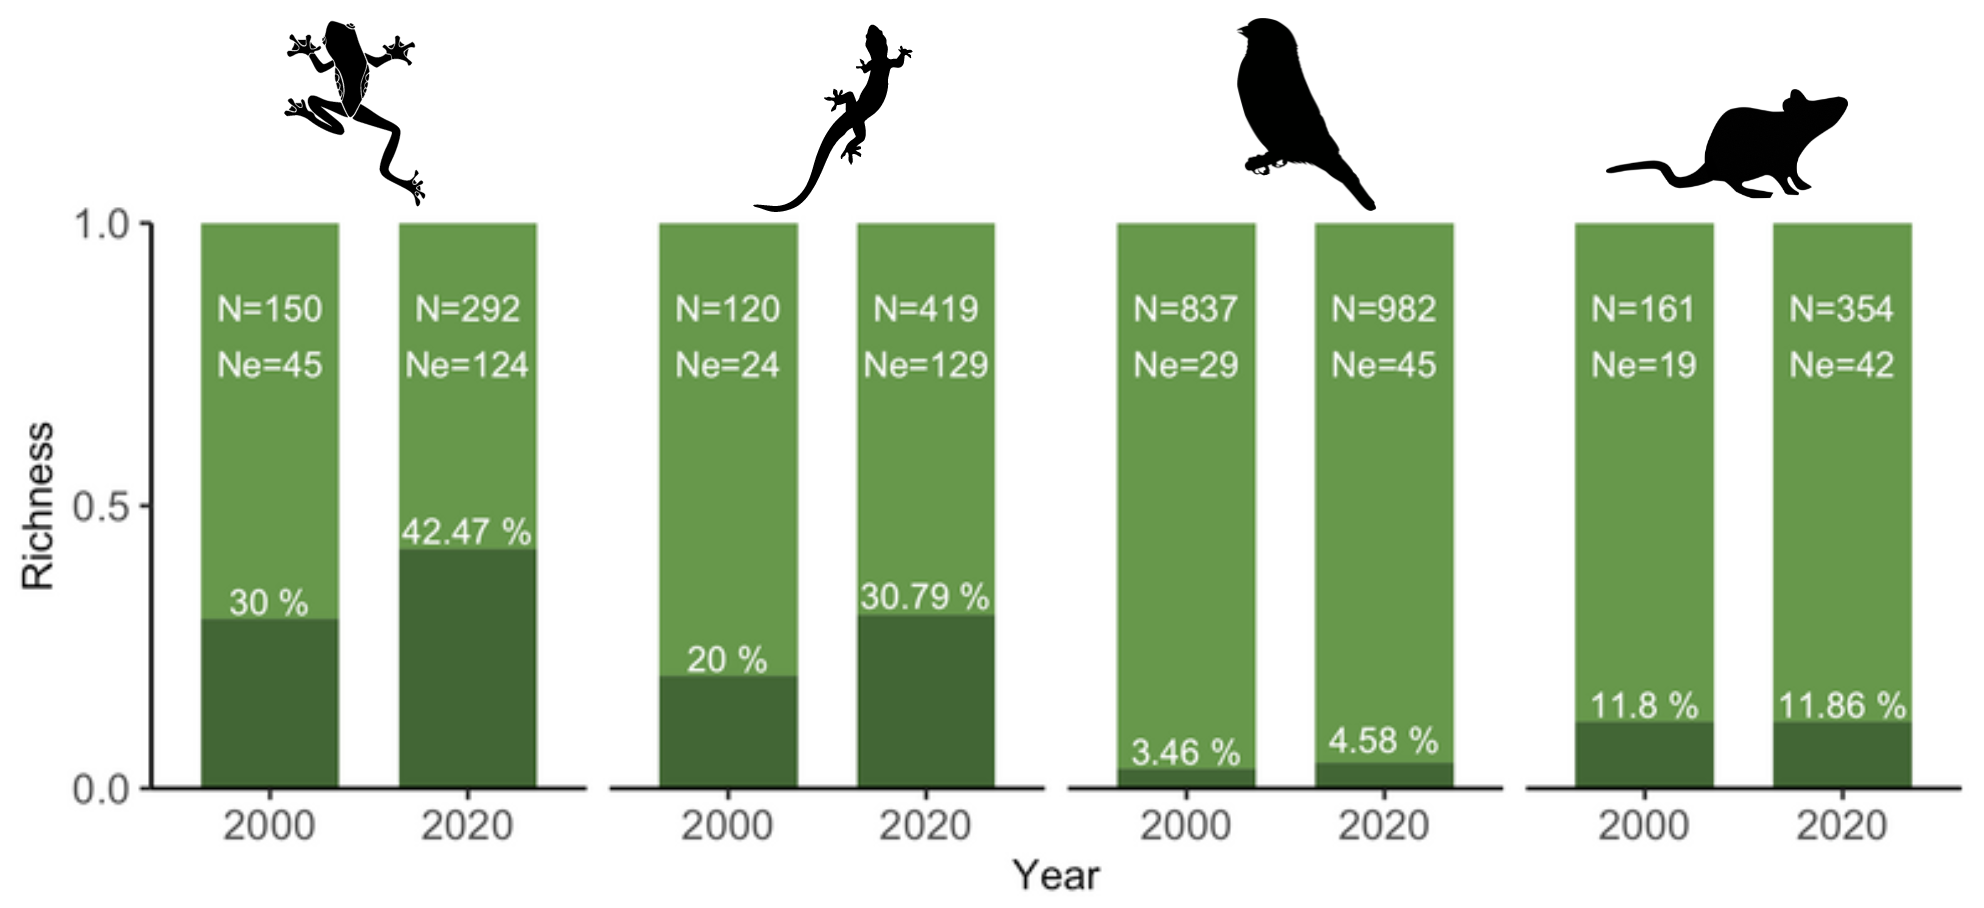
\includegraphics[width=160mm]{Fig c1-1}
	\caption[Rise in endemism levels of Cerrado tetrapods]{\small Numbers and proportions of Cerrado endemic species (dark green) in each tetrapod class in two time slices: 2000 (According to Myers et al. 2000) and 2020 (present study for endemics; ICMBio, 2023 for non-endemics).}
	\label{fig:fig1-1}
\end{figure}

\subsection{\textit{Evolution of taxonomic knowledge}}

Of all 340 Cerrado endemic terrestrial vertebrates, 132 (38.8\%) were described recently, between 2000 and early January 2021, while 137 (40.3\%) were described between 1900-1999, and the remaining 71 taxa (20.9\%) were early descriptions between 1700-1899. The rate of species descriptions since 1820 was of 2.74 species each year but showed a strong acceleration in the last two decades, with an average of six species described each year after the 2000s (\autoref{fig:fig1-2}).

\begin{figure}[htb]
	\centering
	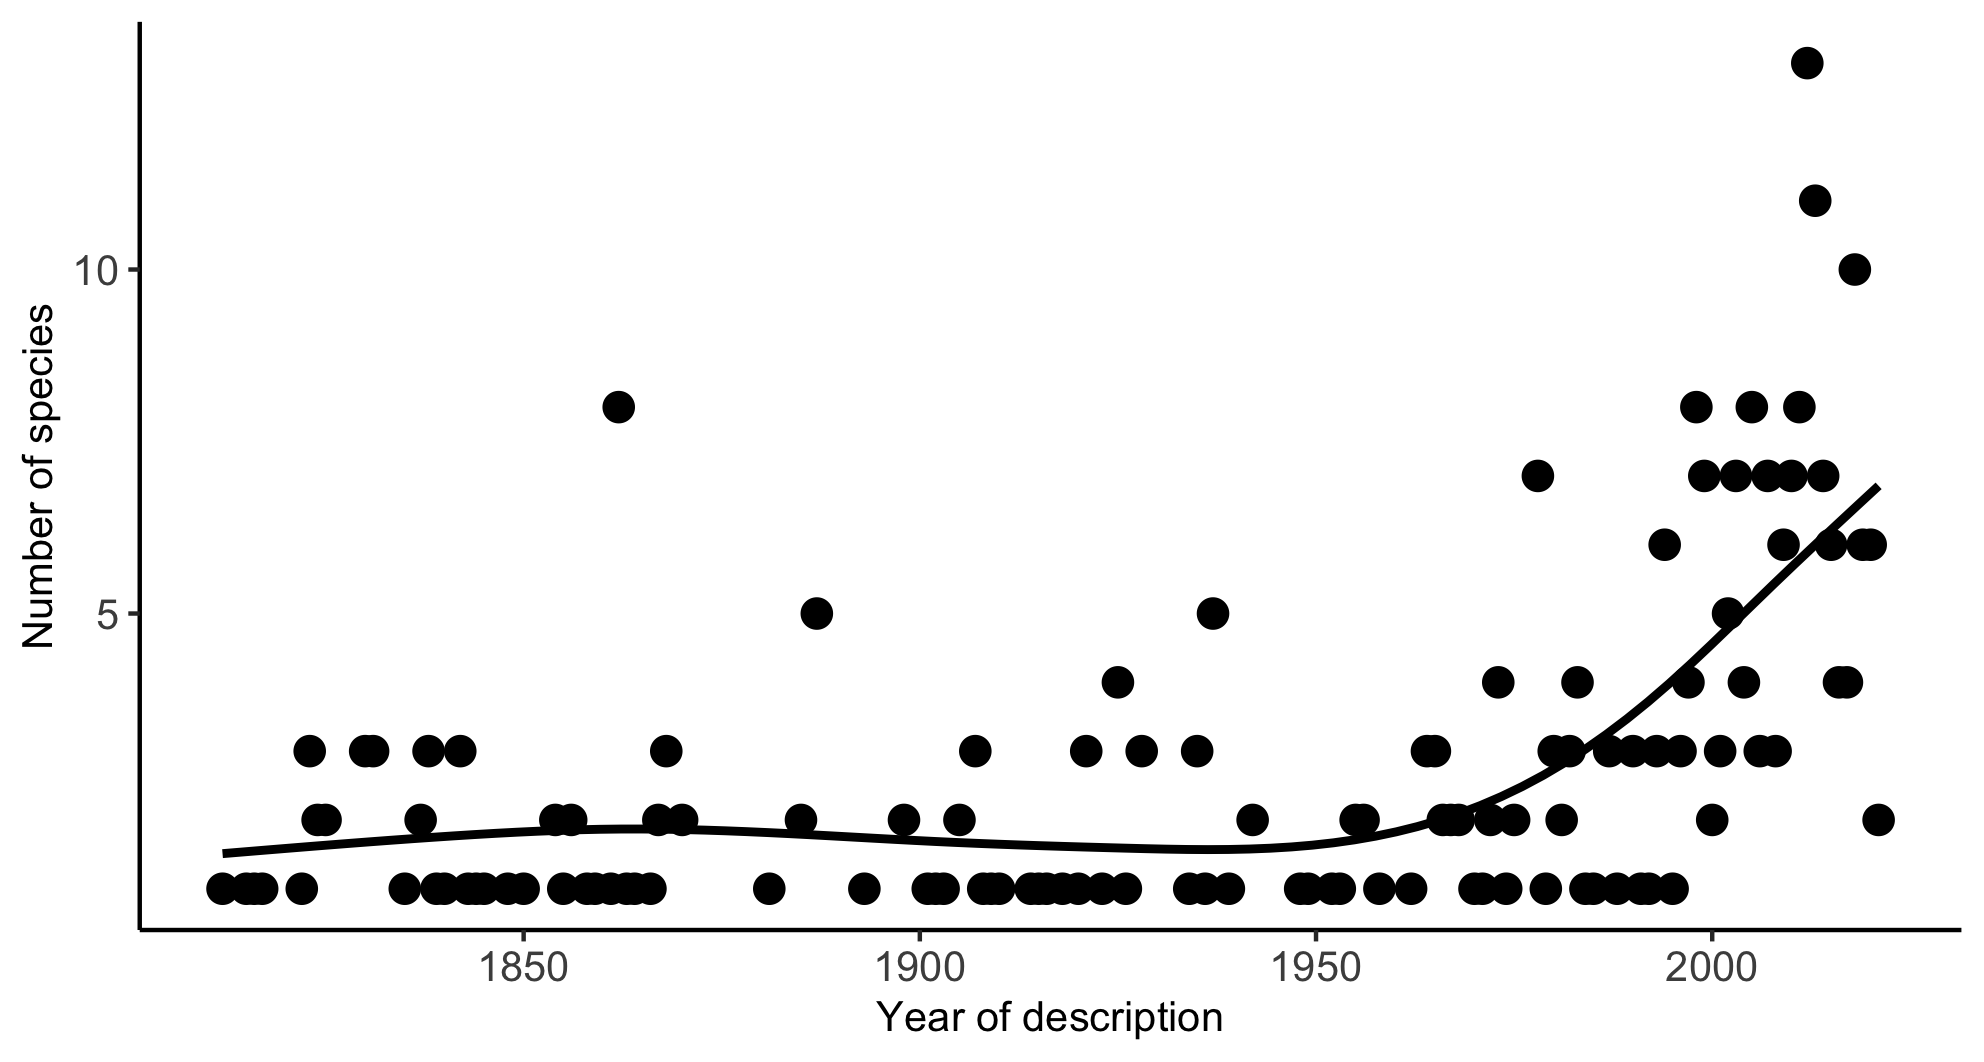
\includegraphics[width=160mm]{Fig c1-2}
	\caption[Number of species described throughout time]{\small Number of species of Cerrado tetrapods described from the early taxonomic studies of the XVIII century to the present.}
	\label{fig:fig1-2}
\end{figure}

\subsection{\textit{Hotspots within hotspots: mapping richness, discovery, habitat loss and protection gap}}

Areas of high endemic species richness are scattered across the Cerrado (\autoref{fig:fig1-3}b), but concentrations of endemics (up to 91 species per cell) were found at the southeastern portion of the Cerrado (Espinhaço range), central Cerrado (Central Brazilian Plateau), southern Cerrado (São Paulo state Cerrado) and western Cerrado (near Chapada dos Guimarães plateau). Most of these areas of high endemic richness are coincident with areas heavily impacted by habitat loss, especially along the southern and southwestern portions of the Cerrado (\autoref{fig:fig1-3}a,b).

Areas of recent (2000-2020) increase in the number of endemics are also scattered across the region (\autoref{fig:fig1-3}c), but higher rates of discoveries were concentrated at the central (Central Brazilian Plateau), eastern (Espinhaço range) and northeastern (Jalapão region and Tocantins river basin) portions of the Cerrado. Except for the northeastern region, most recently described endemics were found in areas already heavily impacted by habitat loss, especially at the central and southeastern portions of the Cerrado (see \autoref{fig:fig1-3}a,c).

\begin{figure}[H]
	\centering
	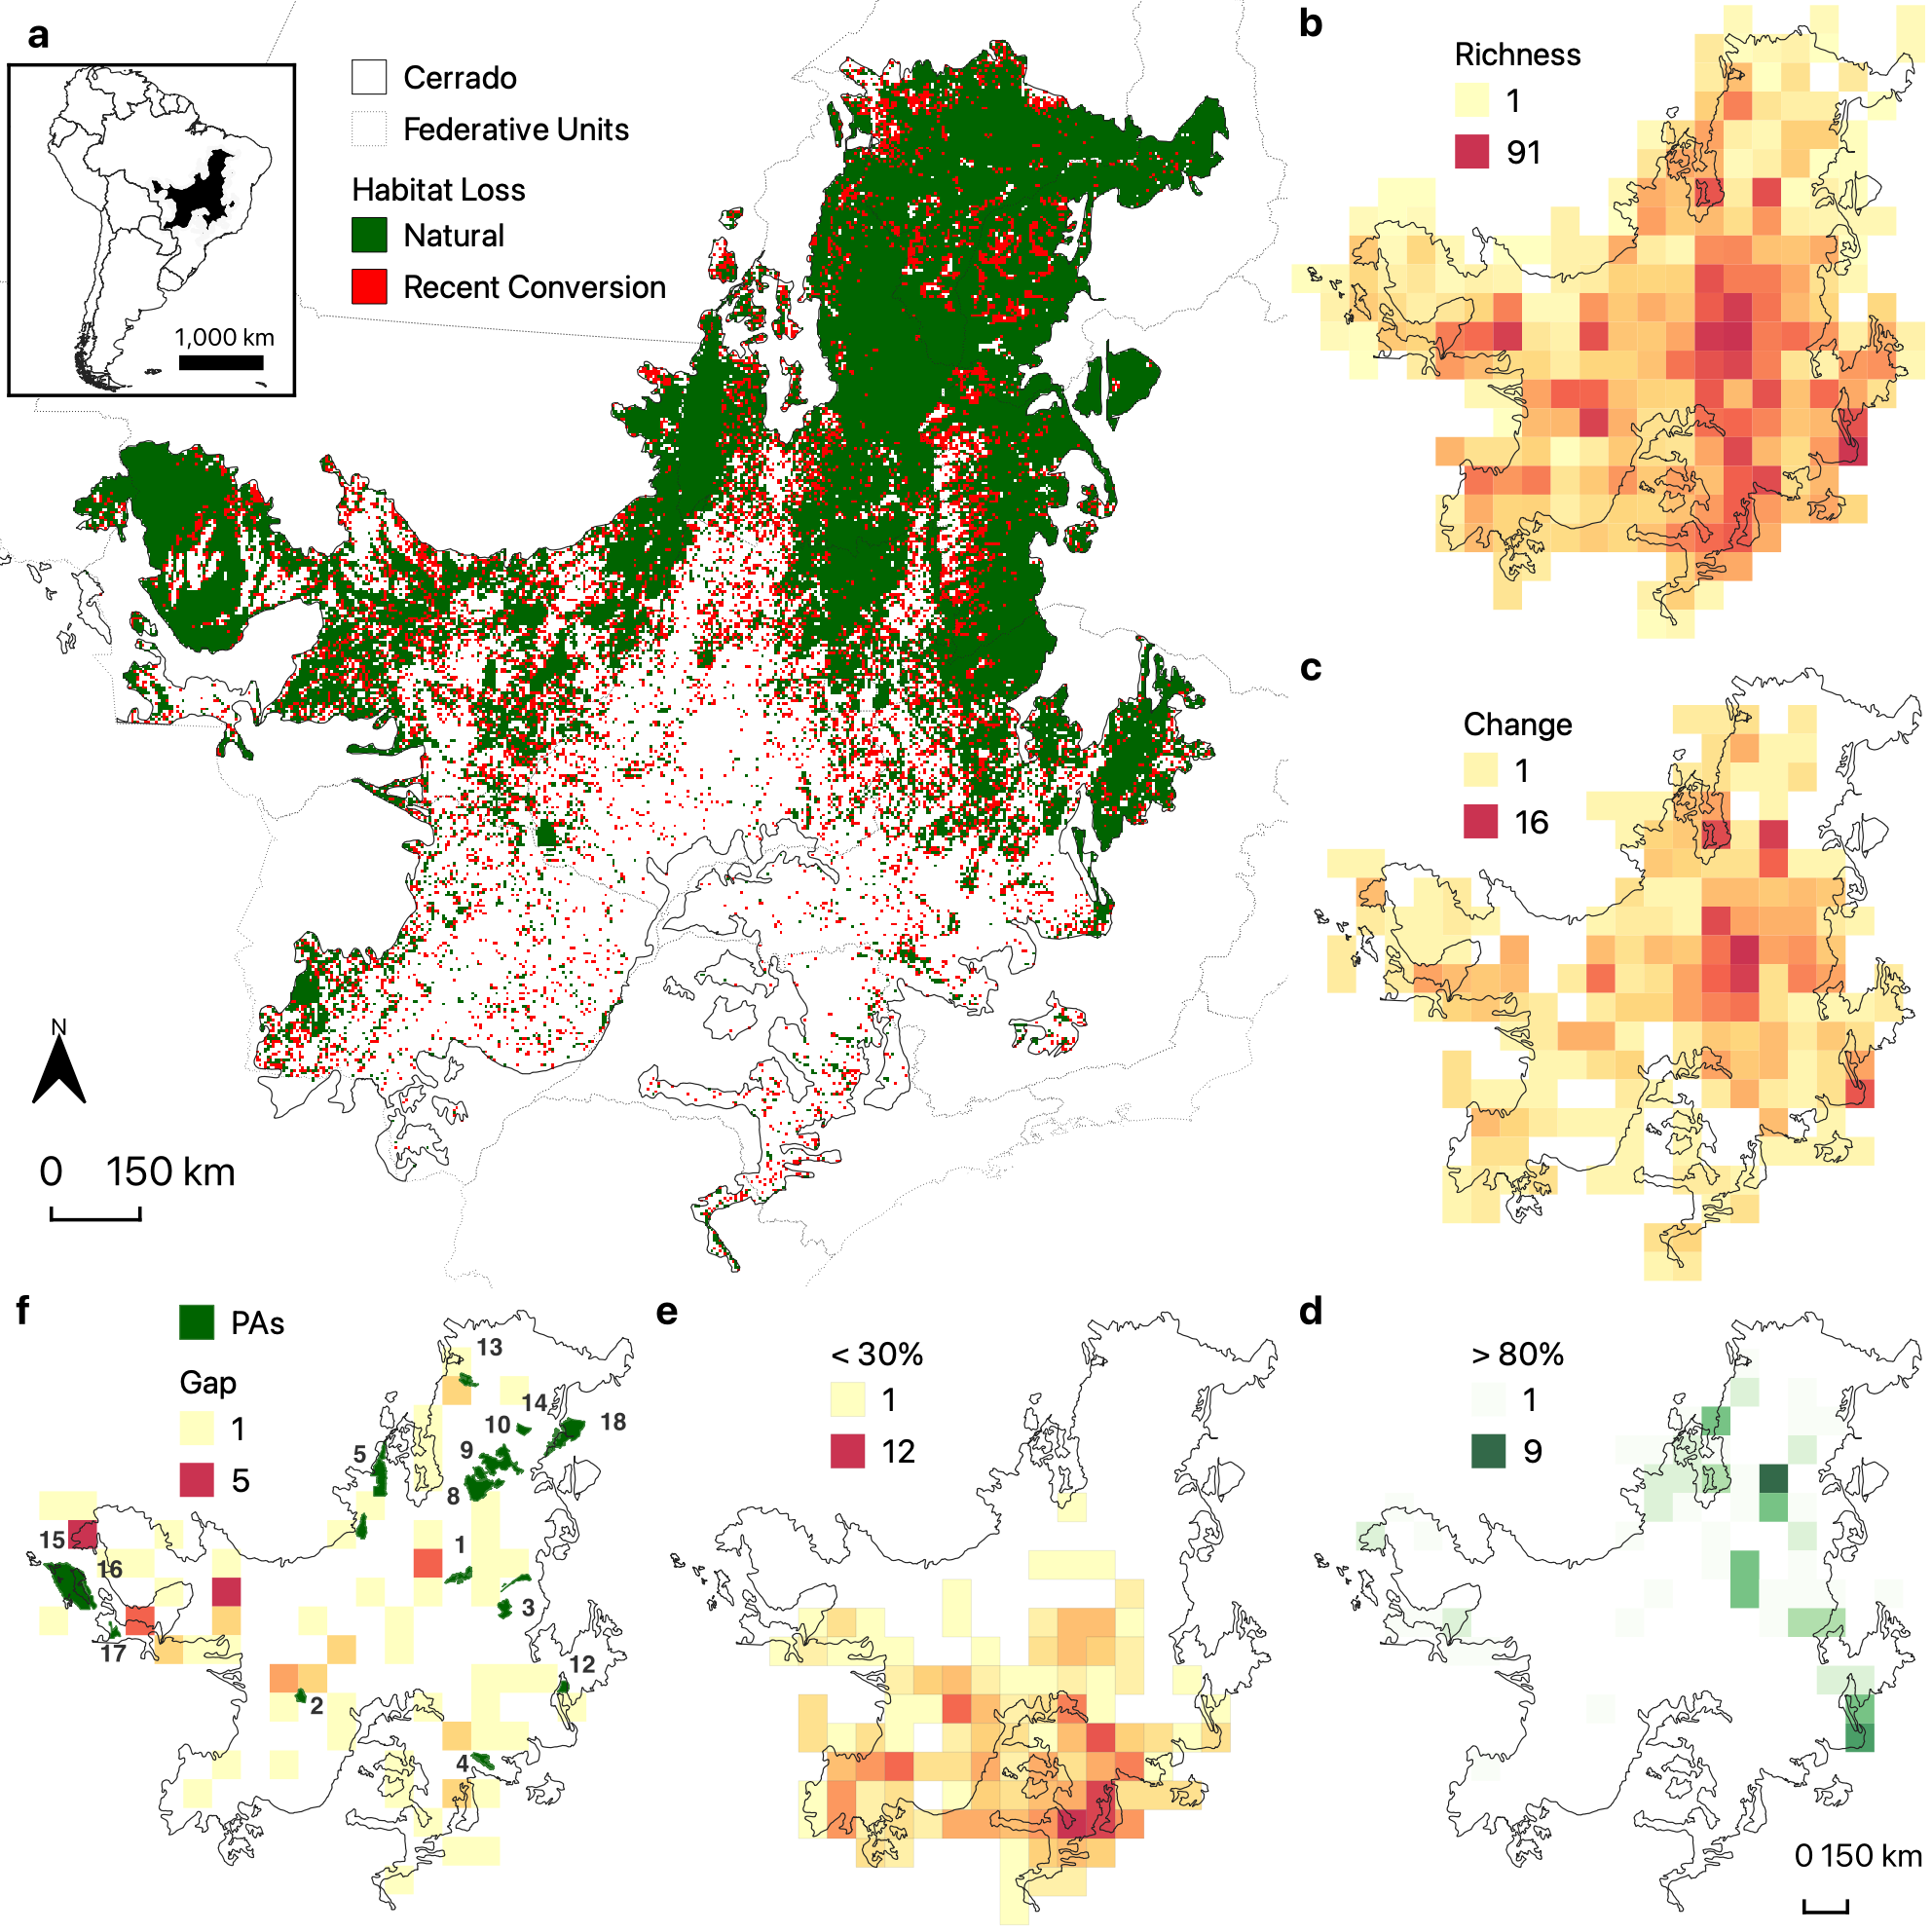
\includegraphics[width=160mm]{Fig c1-3}
	\caption[Habitat loss and Richness maps]{\small Map of land-use and land-cover change from Natural to Anthropic uses in the period from 2000 to 2020, according to MapBiomas (2023) (a). Areas in white within the Cerrado limits were already under anthropic uses in 2000; Endemic tetrapod richness in 2020 (b); Increase in number of endemic tetrapod richness (2000-2020) (c); Endemic tetrapod richness of species least (d, more than 80\% remaining habitats) and most (e, less than 30\% remaining habitats) affected by habitat loss; and Endemic tetrapod gap species (0\% range overlapping PAs) richness (f); Warmer/darker colours indicate higher values. All maps are based on a 1º x 1º grid. Numbers in (f) stand for: 1 - Parque Nacional (PN) da Chapada dos Veadeiros; 2 - PN das Emas; 3 - PN Grande Sertão Veredas; 4 - PN da Serra da Canastra; 5 - Parque Estadual (PE) do Araguaia; 6 - Refúgio de Vida Silvestre Veredas do Oeste Baiano; 7 - Estação Ecológica (EE) Serra Geral do Tocantins; 8 - PN do Araguaia; 9 - PE do Jalapão; 10 - PN das Nascentes do Rio Parnaíba; 11 - PE do Cantão; 12 - PN das Sempre Vivas; 13 - PN da Chapada das Mesas; 14 - EE de Uruçuí-Una; 15 - PN Noel Kempff Mercado; 16 - PE Serra de Ricardo Franco; 17 - PE Serra de Santa Bárbara; and 18 - PN Serra das Confusões.}
	\label{fig:fig1-3}
\end{figure}

A clear north-south division in the Cerrado is visible in maps of species least and most affected by habitat loss (\autoref{fig:fig1-3}d,e). Species with less than 30\% remaining habitats within ranges are concentrated in the southern portion of the Cerrado, while species with more than 80\% remaining habitats within ranges are concentrated in the north and northeastern portions of the region (see \autoref{fig:fig1-3}d,e).



Strict protection PAs started to be designated in the late 50s and the current PA network covers an area of 77,538 km\textsuperscript{2} of which 49,667 km\textsuperscript{2} (64\%) are within the Cerrado limits (representing 2.56\% of the region; see PA area accumulation through time in \nameref{sec:supinfo-1} - \nameref{fig:fig1-s1}). The richest and largest PAs in the Cerrado harbour up to 108 sympatric endemic tetrapod species (\autoref{tab:tab1-1}, see also \autoref{fig:fig1-3}f) and can be pointed as candidate Key Biodiversity Areas (KBAs, \citealp[see][]{KBAs2022}) for safeguarding Cerrado endemic tetrapods, with Parque Nacional Chapada dos Veadeiros, Parque Nacional das Emas, Parque Nacional Grande Sertão Veredas and Parque Nacional da Serra da Canastra harbouring the richest Cerrado endemic tetrapod faunas (See \autoref{tab:tab1-1}). 

\begin{table}[h]
	\centering
	\caption[Richest Cerrado Strict Protected Areas]{Richest strict protection PAs in terms of Cerrado endemic terrestrial vertebrates. All strict protection PAs with more than 100,000 ha are listed. Code = PA code ID linked to \autoref{fig:fig1-3}f; Year = Year of PA creation; N = Number of Cerrado endemic terrestrial vertebrates whose geographical range intersects with PA limits; Area is calculated in hectares (ha).}
	\label{tab:tab1-1}
	\vspace{\bigskipamount}
	\footnotesize
	\begin{tabular}{cllccc}
		\hline
		Code & Name & Designation & Year & N & Area (ha) \\
		\hline
		1 & Parque Nacional Chapada dos Veadeiros & National Park & 1961 & 108 & 240,585 \\
		2 & Parque Nacional das Emas & National Park & 1961 & 99 & 132,785 \\
		3 & Parque Nacional Grande Sertão Veredas & National Park & 1989 & 94 & 230,854 \\
		4 & Parque Nacional da Serra da Canastra & National Park & 1972 & 84 & 197,971 \\
		5 & Parque Estadual do Araguaia & State Park & 2001 & 78 & 229,921 \\
		6 & Refúgio de Vida Silvestre Veredas do Oeste Baiano & Wildlife Refuge & 2002 & 78 & 128,050 \\
		7 & Estação Ecológica Serra Geral do Tocantins & Ecological Station & 2001 & 77 & 707,087 \\
		8 & Parque Nacional do Araguaia & National Park & 1959 & 75 & 555,503 \\
		9 & Parque Estadual do Jalapão & State Park & 2001 & 65 & 158,972 \\
		10 & Parque Nacional das Nascentes do Rio Parnaíba & National Park & 2002 & 60 & 749,770 \\
		11 & Parque Estadual do Cantão & State Park & 1998 & 60 & 100,414 \\
		12 & Parque Nacional das Sempre Vivas & National Park & 2002 & 57 & 124,156 \\
		13 & Parque Nacional da Chapada das Mesas & National Park & 2005 & 46 & 159,953 \\
		14 & Estação Ecológica de Uruçuí-Una & Ecological Station & 1981 & 41 & 135,125 \\
		15 & Parque Nacional Noel Kempff Mercado & National Park & 1979 & 37 & 1,617,204 \\
		16 & Parque Estadual Serra de Ricardo Franco & State Park & 1997 & 36 & 157,831 \\
		17 & Parque Estadual Serra de Santa Bárbara & State Park & 1997 & 33 & 120,432 \\
		18 & Parque Nacional Serra das Confusões & National Park & 1998 & 27 & 823,845 \\
		\hline
	\end{tabular}
\end{table}

However, amongst the 340 endemic species analysed, 296 (87.05\%) are poorly represented in the PA system, with less than 17\% (i.e. Aichi Target) of their ranges represented in strict protection reserves. Of those, 129 (43.58\%) are restricted range species, 142 (47.97\%) are partially ranged, and 25 (8.44\%) are widespread endemic species. A total of 51 (15\%) species are completely absent from PAs (hereafter, gap species, \autoref{fig:fig1-3}f). Most (47; 92.15\%) of the gap species are restricted-range taxa occurring allopatrically, especially in the western portion of the Cerrado (\autoref{fig:fig1-3}f), while the remaining 4 (7.85\%) are partially ranged species. The northeastern portion of the Cerrado shows only a few gap species, being the least affected by habitat loss (see \autoref{fig:fig1-3}d) and harbouring the largest PAs (see \autoref{fig:fig1-3}f). Considering gap species in the Brazilian official Red List \citep{ICMBio2023}, DD was the most frequent category, applied to 24 (47\%) species, followed by LC (21.5\%) and EN (7.84\%). Six (11.7\%) gap species were not assessed by \citet{ICMBio2023}.

\subsection{\textit{Range size, habitat loss, protection and threat levels of Cerrado endemic tetrapods}}

Most Cerrado endemic tetrapods are not widespread in the Cerrado, showing restricted (49.7\%) or partial (42.9\%) ranges. Range sizes are significantly different among Cerrado tetrapod classes (Kruskal-Wallis $\chi^2$ = 31.76, \textit{df} = 3, \textit{p} <0.001), with anurans and reptiles tending to show smaller ranges than mammals and birds (see \nameref{sec:supinfo-1} - \nameref{fig:fig1-s2}). Two species (\textit{Hylaeamys acritus} and \textit{Juscelinomys huanchacae}, both considered DD in the global Red List) were not assessed for land cover, as their ranges are outside the Brazilian border, in areas lacking MapBiomas land-use classification. Amongst the remaining 338 species, a total of 294 (86.98\%) have lost natural habitats within their range between 2000 and 2020, with an average of 8\% of loss, ranging from 0.1\% to a maximum of 45\% (\nameref{sec:supinfo-1} - \nameref{sup:1-s1}). Habitat loss affected 129 (43.87\%), 140 (47.61\%) and 25 (8.5\%) species with restricted, partial and widespread geographical ranges, respectively. On the other hand, 39 species (11.5\%) showed marginal gains (an average of 4.63\%) in natural habitats within their ranges (\nameref{sec:supinfo-1} - \nameref{sup:1-s1}). Details on species range categories, natural habitat modification (gain or loss), and range protection categories can be found in \nameref{sec:supinfo-1} - \nameref{fig:fig1-s2}.

A total of 265 species (77.9\%) were assessed by the IUCN Red List, while 315 (92.6\%) were assessed in the Brazilian official Red List (both using the same IUCN categories and criteria, \autoref{fig:fig1-4}). Birds are, proportionally, the most threatened tetrapod class, followed by mammals and reptiles, with amphibians being the least threatened in both lists (see \autoref{fig:fig1-4}a). Proportions of DD species in the IUCN Red List were always higher than those in the Brazilian assessment. In the global IUCN Red List, the percentage of DD species was higher for amphibians (43.9\%), followed by reptiles (27.41\%) and mammals (18.91\%), while in the Brazilian official Red List proportions of DD species peaked in reptiles (15.65\%), followed by mammals (10.81\%) and amphibians (9.32\%). Due to the higher number of assessed species, more recent completion date and smaller proportion of DD species, the following results are all based on the Brazilian official Red List \citep{ICMBio2023}.

\begin{figure}[H]
	\centering
	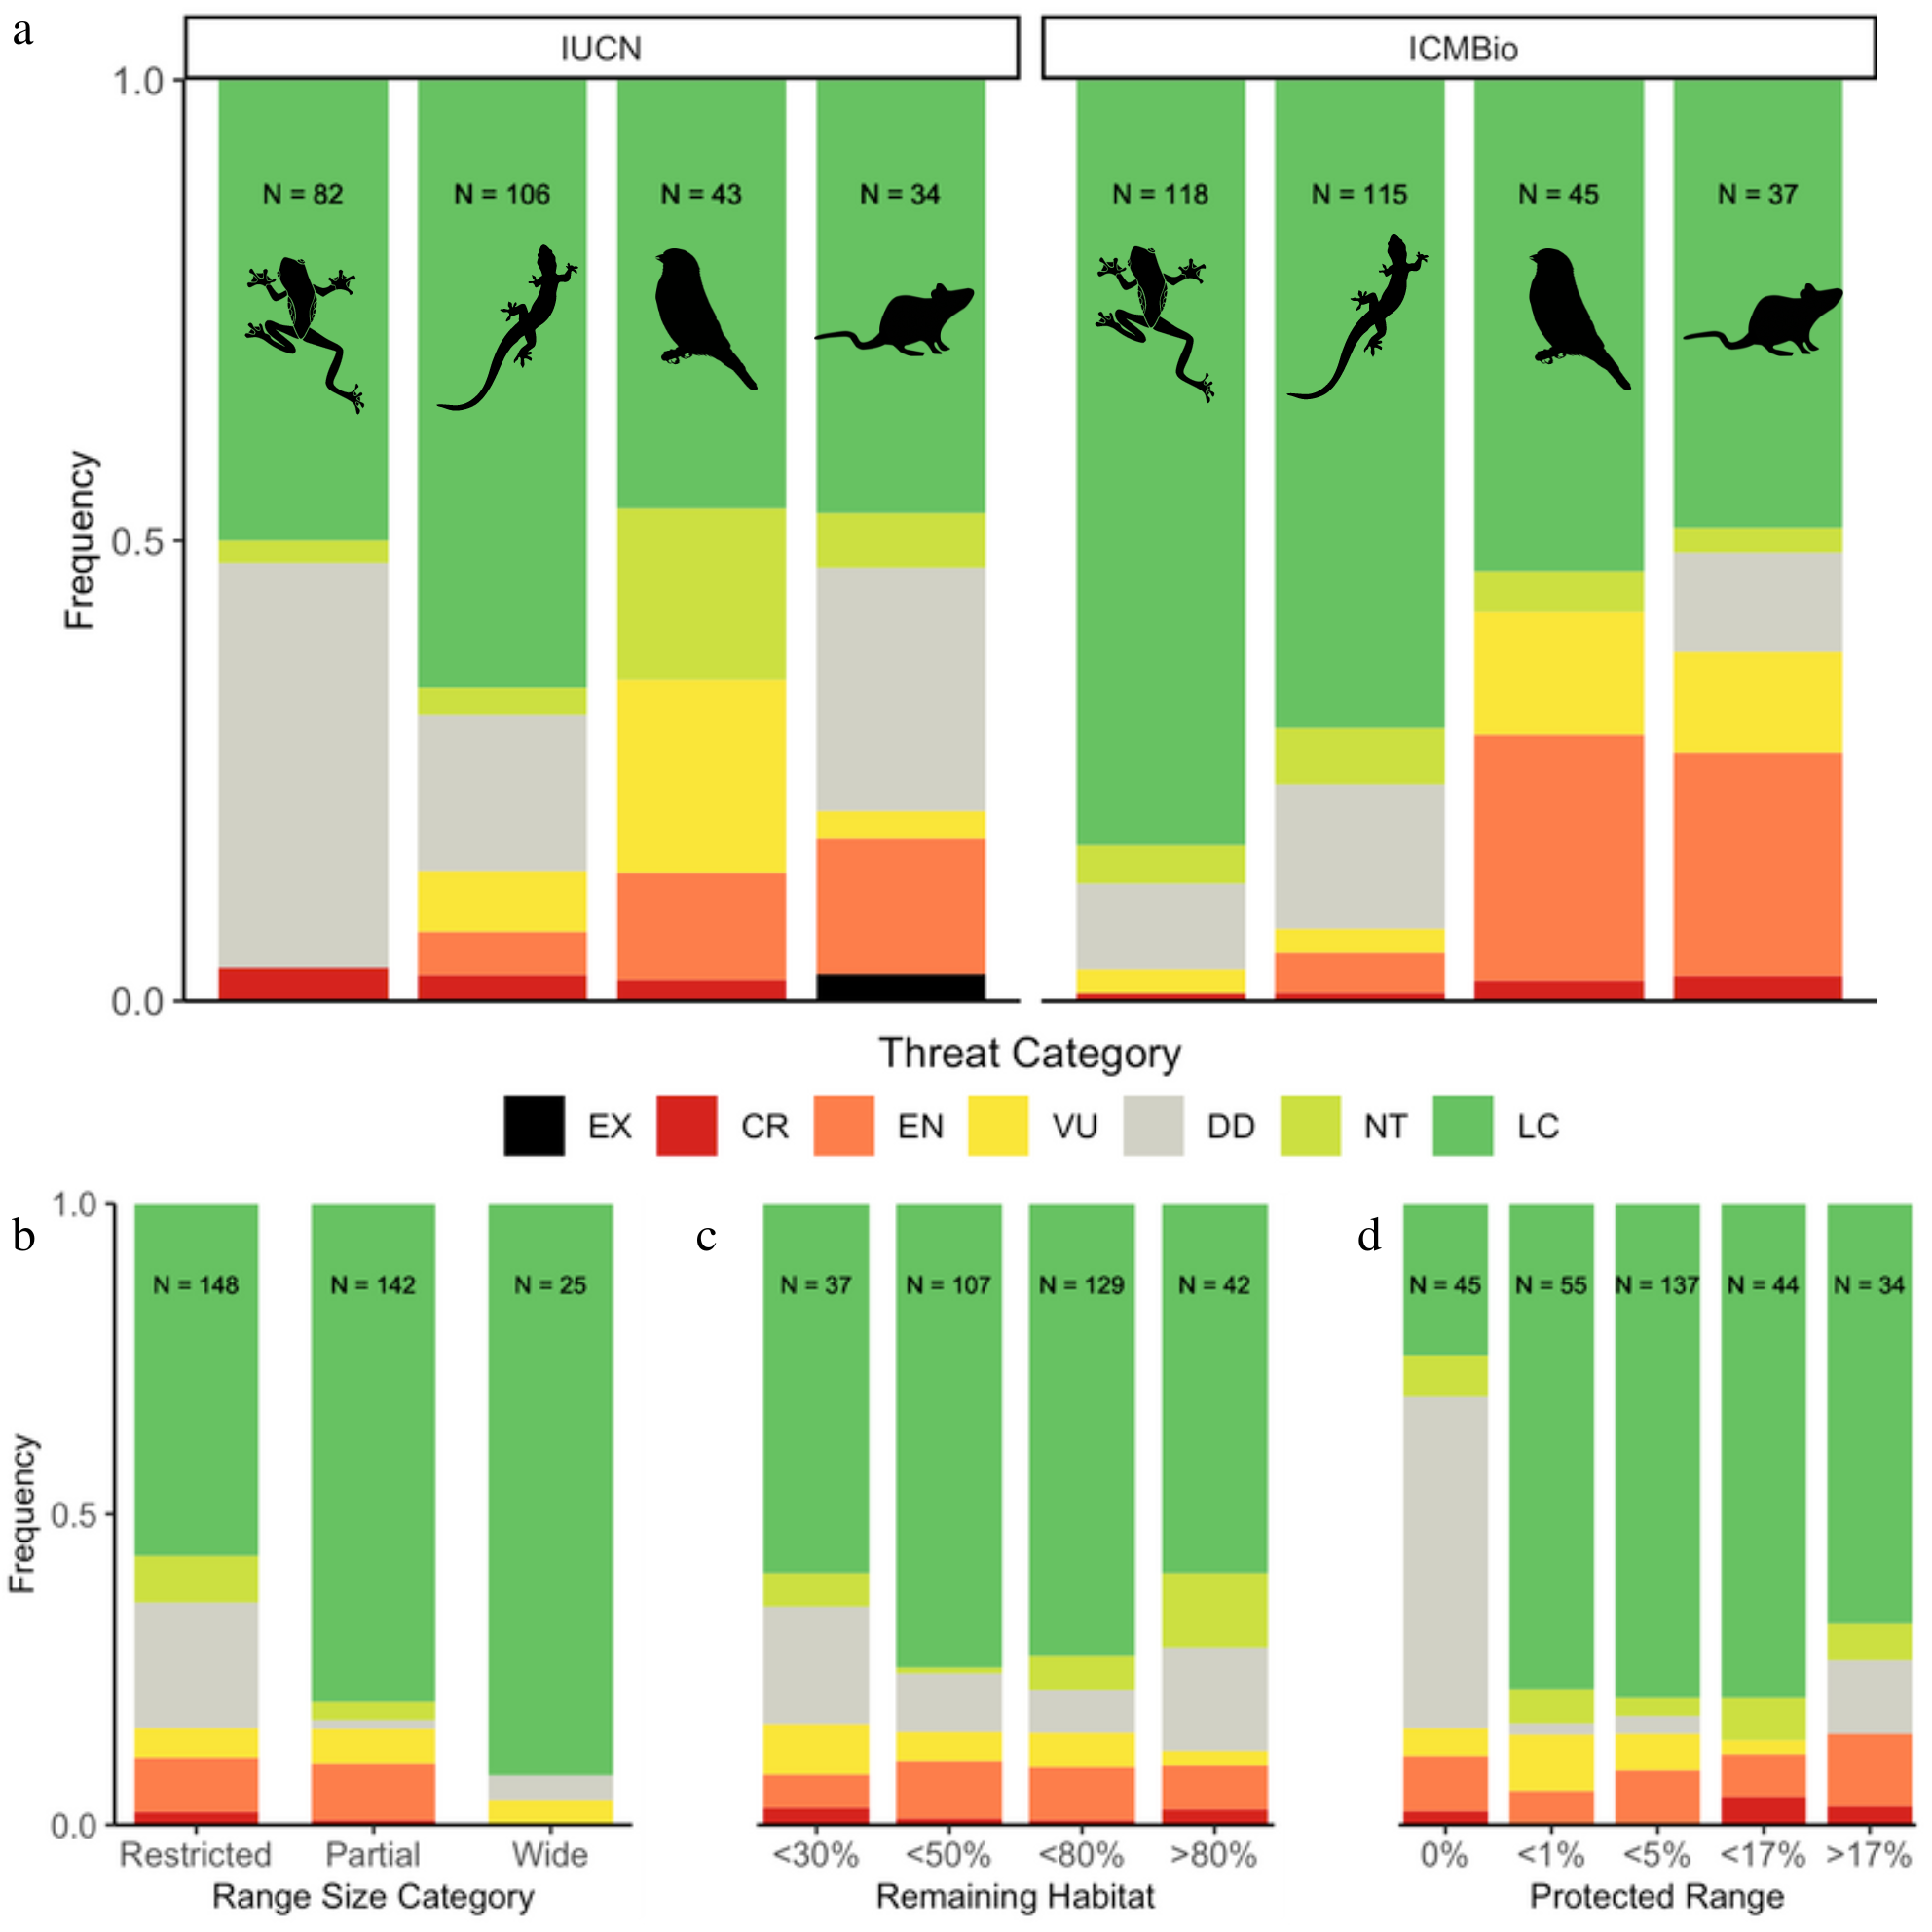
\includegraphics[width=160mm]{Fig c1-4}
	\caption[Threat assessments against range-size, habitat loss, and protection]{\small Proportion and numbers of endemic tetrapod species in each IUCN category, according to the IUCN global Red List (N = 265) and the Brazilian official Red List (N = 315) (a); and according to range size (b), percentage of remaining habitat (c), and percentage of protection on PAs (IUCN categories I-IV, d). Categories in figures 4b, c and d, follow the Brazilian official Red List (N = 315).}
	\label{fig:fig1-4}
\end{figure}

Proportions of species in threat categories were significantly different among tetrapod classes ($\chi^2$ = 54.52; \textit{df} = 3; \textit{p} < 0.001), being higher in birds (42.2\%) and mammals (37.8\%) than in amphibians (3.38\%) and reptiles (7.82\%). The proportion of threatened and DD species was higher among restricted-range or partially ranged species than in widespread taxa, the majority of which were assessed as LC (\autoref{fig:fig1-4}b). Threatened and non-threatened species in the Brazilian official Red List showed no significant differences in range size (Kruskal-Wallis $\chi^2$ = 0,000039, \textit{df} = 1; \textit{p} = 0.99). However, range sizes were significantly different if we considered all IUCN categories (Kruskal-Wallis $\chi^2$  = 48.04, \textit{df} = 5; \textit{p} < 0.001), with Vulnerable birds and mammals showing large ranges, while species assessed as Critically Endangered, Vulnerable amphibians,  and data-deficient reptiles often showing small ranges (\nameref{sec:supinfo-1} - \nameref{fig:fig1-s3}).

Proportions of threatened and DD species seem poorly related to levels of habitat loss, although the percentage of threatened species was slightly higher in species showing less than 30\% remaining habitat (\autoref{fig:fig1-4}c). Threatened and non-threatened (binary test) species in the Brazilian official Red List showed no significant differences in the percentage of remaining habitat within ranges (Kruskal-Wallis $\chi^2$ = 0.33, \textit{df} = 1; \textit{p} = 0.56). Moreover, species assigned to different threat categories (including all categories) also showed no significant differences in the percentage of remaining habitat (Kruskal-Wallis $\chi^2$ = 5.63, \textit{df} = 5; \textit{p} = 0.34; \nameref{sec:supinfo-1} - \nameref{fig:fig1-s4}).

Proportions of threatened and non-threatened species also seem poorly related to levels of protection (\autoref{fig:fig1-4}d). However, the proportion of DD species is noticeably higher in gap species (see \autoref{fig:fig1-4}d). Threatened and non-threatened (binary test) species in the Brazilian official Red List showed no significant differences in protection within ranges (Kruskal-Wallis $\chi^2$ = 0,75, \textit{df} = 1; \textit{p} = 0.38). However, species assigned to different IUCN categories (including all categories) differed in the percentage of protection within ranges (Kruskal-Wallis $\chi^2$ = 36.146, \textit{df} = 5; \textit{p} < 0.001), with some Least Concern species showing a higher proportion of protected ranges (\nameref{sec:supinfo-1} - \nameref{fig:fig1-s5}).

\subsection{\textit{Vulnerability, Irreplaceability and Discovery}}

We observed a significant negative correlation between range size and date of species descriptions: recently described endemics tended to show localised, narrow ranges, while species described in early taxonomic studies tended to be widespread (F\textsubscript{1, 313} = 48.19, R\textsuperscript{2} = 0.1334,  \textit{p} < 0.001; \autoref{fig:fig1-5}a). Threatened and non-threatened species seem scattered among different description dates and range sizes. However, the DD category was concentrated in species with recent descriptions, especially amphibians and reptiles (see \autoref{fig:fig1-5}a).

Threatened species also seem relatively scattered according to range size and proportion of habitat loss (\autoref{fig:fig1-5}b). However, many DD species (especially amphibians and reptiles) showed narrow ranges (see \autoref{fig:fig1-5}b and \autoref{fig:fig1-4}c), including species heavily impacted by habitat loss (see \autoref{fig:fig1-5}b). Moreover, all CR species were concentrated in the left portion of the graph, showing restricted ranges (see \autoref{fig:fig1-5}b and \autoref{fig:fig1-4}c).

\begin{figure}[H]
	\centering
	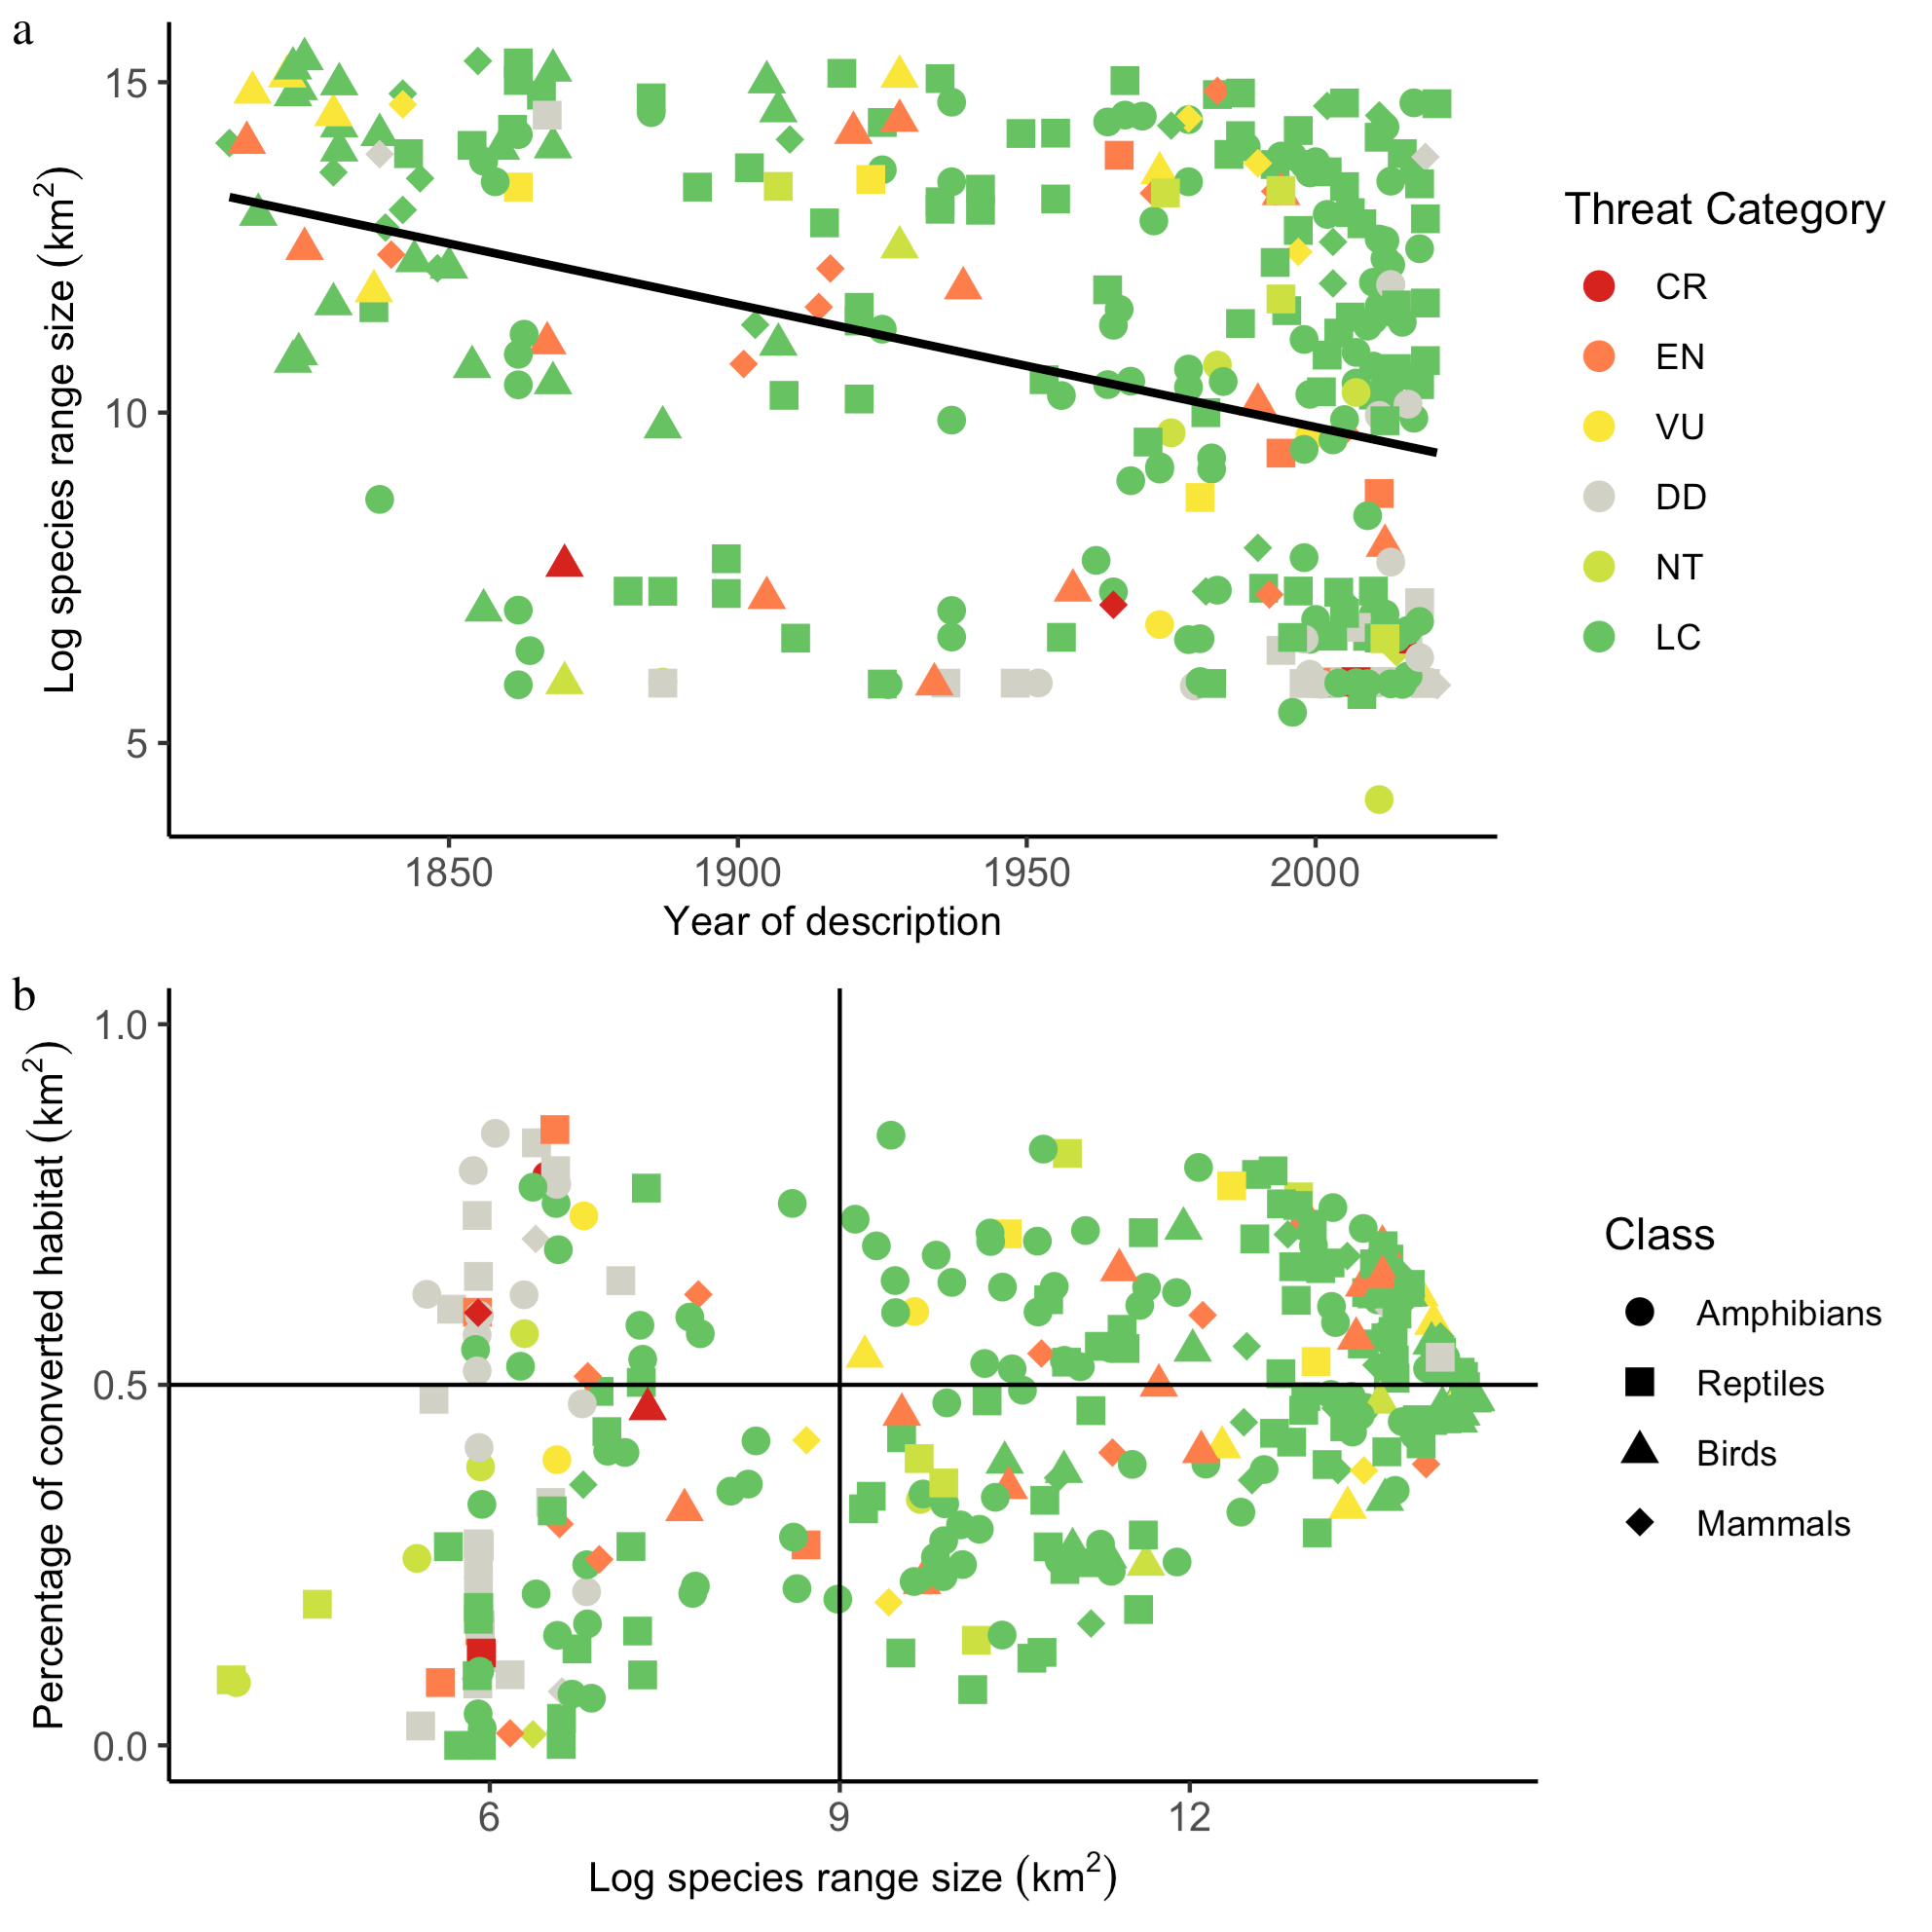
\includegraphics[width=160mm]{Fig c1-5}
	\caption[Range-size, description date and habitat loss]{\small Relationship between range size and date of description (a) and percentage of remaining habitat within ranges (b) of Cerrado endemic tetrapods. Symbols indicate tetrapod classes and colours indicate IUCN categories in the Brazilian official Red List (ICMBio, 2023).}
	\label{fig:fig1-5}
\end{figure}

\section{Discussion}

The so-called Linnean Shortfall (e.g. lack of knowledge on actual species diversity; \citealp{Hortal2015}) has long been claimed to preclude proper conservation planning, especially at refined scales \citep{Whittaker2005}. Knowledge on terrestrial vertebrates and the predicted diversity of the best-known animal groups on the planet \citep{Brown1995} proved to be highly underestimated in the Cerrado at the time of the classic hotspot paper \citep{Myers2000}. Since 2000 however, basic biodiversity knowledge in the Cerrado has improved significantly, both in quality and quantity. In fact, more than one-third of all currently known endemic terrestrial vertebrate species were described in the last two decades. Herein we show that both vulnerability and irreplaceability levels have risen sharply in the Cerrado. Recent field efforts, directed towards sampling gaps, coupled with resulting taxonomic advances, were determinant to the steep rise in vertebrate diversity knowledge in the last 20 years, both in poorly known regions, like northern Cerrado, as in highly sampled areas such as the Espinhaço Mountain Range, or Central Brazilian plateau \citep{Nogueira2009, Nogueira2010, Valdujo2012, Azevedo2016, Nogueira2019, Carmignotto2022}.

Our results, however, indicate that the pace of taxonomic and biogeographical discovery in the Cerrado has not been coupled with effective conservation action on the ground. The recent increase in taxonomic knowledge results in the detection of highly complex, endemic and highly threatened biotas, still marginally represented in protected areas and under persistent pressure of habitat loss resulting from large-scale changes in land use after the expansion of the agricultural frontier in central Brazil (\citealp{Pacheco2021}; \citealp[see also][]{VieiraAlencar2023}), continuing a trend already detected in the late XXth century \citep{Ratter1997, KlinkMachado2005}. Hence, the coupled increase in endemism and habitat loss results in the detection of highly vulnerable and irreplaceable taxa and areas, already largely impacted by habitat loss and fragmentation \citep{Strassburg2017, VieiraAlencar2023}.

Our results reinforce previously detected conservation prioritizations in northern Cerrado (\citealp[e.g.][]{Monteiro2020, VieiraAlencar2023}) and the urgency to take action and to secure the last opportunities to safeguard the last continuous areas of preserved Cerrado \citep{VieiraAlencar2023}. However, conservation action should also be directed to safeguarding the last remnants of Cerrado in southeastern Brazil, regardless of their size and current connectivity, given that these highly impacted and fragmented regions harbour many threatened or restricted-range Cerrado endemics, and may serve as important backbones to the implementation of restoration programmes \citep{Strassburg2017, VieiraAlencar2023}.

A recent study on the interactions between the effects of Linnean and Wallacean shortfalls on species threat \citep{Baranzelli2023} indicates that increased knowledge on species distribution and increased taxonomic knowledge have antagonistic effects on threat perception: while a higher number of described species indicate increased threats, the detection of new range data and wider distributions lead to decreased threat perception. However, our results indicate that most new data on species ranges result in better taxonomic resolution and the detection of smaller, local ranges, and not more widespread taxa. In other words, the more we understand ranges, the more species are described, either as a result of splitting previous ranges or via the detection of allopatric, peripheral, isolated new taxa and populations \citep{Nogueira2011, Azevedo2016}. Moreover, even new records of restricted-range endemic tetrapods from the highly impacted southern Cerrado will still come from extremely small and isolated fragments of Cerrado (\citealp[see][]{Serrano2023}) describing very impacted populations prone to extinction in the next few decades \citep{Strassburg2017}.

In sum, our data indicate that Cerrado endemic tetrapods, including the many recently discovered and described restricted-range taxa, are at great risk of a severe cycle of extinction in the next few decades. In fact, ca. 480 endemic Cerrado vascular plant species are estimated to become extinct in the near future (until 2050) if current rates of habitat loss and conversion to croplands are not urgently halted and reversed in central Brazilian savannas \citep{Strassburg2017}. Even worse, at least one-third of Cerrado’s plant species distribution within PAs is predicted to be lost due to climate change alone, considering the most optimistic scenario forecasted for 2050 and 2080 \citep{Velazco2019}, with habitat loss predicted to potentially increase this effect for non-protected species ranges. The highest losses are predicted to occur where the greatest species richness is harboured, more specifically the central and central-eastern areas of the Cerrado, where we also detected high levels of overall richness and new species descriptions (\autoref{fig:fig1-3}b,c). However, given that the rise in tetrapod endemism spans a wider portion of the Cerrado (see \autoref{fig:fig1-3}c), exceeding areas of plant extinctions hotspots, we argue that the figures for Cerrado tetrapods will be even more sombre than that detected for vascular plants. As an example, areas such as the southern portion of the Serra Geral plateau, with high rates of discovery in Cerrado tetrapods and harbouring recently described species that have lost more than 40\% of their known ranges (e.g. \textit{Amphisbaena persephone}, \textit{Amphisbaena carli}, see \nameref{sec:supinfo-1} - \nameref{sup:1-s1}) were not targeted as an area of future extinctions or as a priority area for Cerrado restoration \citep{Strassburg2017}.

Moreover, given the high structural heterogeneity of Cerrado habitats, ranging from open grasslands to wetlands and dense woodlands and forests and the noticeable habitat specialisation of many Cerrado species (\citealp[see][]{Silva2002, Nogueira2009, Nogueira2011}), habitat requirements of Cerrado tetrapods should be a major element in guiding restoration and habitat protection. As an example, restoring arboreal vegetation in areas originally dominated by fire-prone grasslands may be inefficient and even deleterious to grassland specialists. Both the protection and restoration of the Cerrado habitat must be directed to preserving the original habitat mosaic that typifies the domain of central Brazilian savannas (\citealp[see][]{Silva2002}). The conservation of Cerrado endemic tetrapods depends both on the small or currently disconnected fragments (such as those in the Southern Cerrado) as on the larger connected northern Cerrado areas. Protecting and halting deforestation in both these land use scenarios is mandatory to avoid extinction and collapse of Cerrado biological diversity in the coming decades \citep{VieiraAlencar2023}.

The recent accumulation of taxonomic and biogeographical knowledge in the Cerrado also seems poorly reflected in species threat assessments. Despite the very important advances in biodiversity assessments worldwide and specifically in Brazil (12,254 species assessed in the last two decades, an unparalleled effort worldwide; \citealp{ICMBio2018}), many recently described, restricted-range species are still classified as DD in official Red Lists (either national or global) or have not been assessed yet. This large number of unassessed and DD species may explain the low proportions of threatened species of Cerrado anurans and reptiles. These low proportions of threatened species are not compatible with expected values based on the proportion of threatened species in the global Red List (40.7\% in amphibians; 21.1\% in reptiles, \citealp[see][]{Cox2022, Borgelt2022}). If the proportion of threatened Cerrado amphibians and reptiles followed the proportions on the global Red List, we would have 48 threatened amphibians and 24 reptiles in the list of threatened Cerrado endemic tetrapods. However, in the most recent and complete assessment (the Brazilian Official Red List, \citealp{ICMBio2023}), only four amphibians and nine reptiles were classified as threatened, in apparently highly underestimated figures.

Moreover, the proportions of threatened species among tetrapod classes in the Cerrado are highly heterogeneous. In contrast, global data indicate that for most (87\%) terrestrial regions no tetrapod class is disproportionately threatened compared with the other classes \citep{Cox2022}. Hence, our results in the Cerrado disagree with a global trend of high geographical concordance of threat levels in all four tetrapod classes. On the contrary, our results show that species of amphibians and reptiles show much lower proportions of threatened species than Cerrado birds and mammals, resulting in underestimated lists of threatened Cerrado tetrapods.

A recent study, using models that suggest Red List categories or probabilities of threat for DD species concluded that 85\% of amphibians, 59\% of reptiles and 61\% of mammals currently assessed as DD could be reassessed in a threat category (VU, EN or CR), based on the available threat and range data (\citealp[see][]{Borgelt2022}). Applying these proportions to our numbers of DD species would result in the addition of  22 species (+6\%) to the list of threatened Cerrado tetrapods, including nine amphibians, 11 reptiles and two mammals. Also alarming is the number of species not even assessed regarding their threat status. If the 25 described endemics species absent from the Brazilian Red List were to be assessed in a threat category using the same predictions estimated for DD species \citep{Borgelt2022}, another 16 species (five amphibians, eight reptiles and three mammals) would be included in the final threatened Cerrado endemic tetrapods species list. These combined comparisons indicate that, despite the clear advances in biodiversity documentation (species discoveries, new inventories, improved knowledge on ranges and endemism), the number of threatened tetrapod species is still grossly underestimated in the Cerrado.

We see little biological meaning in the fact that so few Cerrado amphibians and reptiles are assessed as threatened compared to birds and mammals. Given the tendency for amphibians and reptiles to show relatively restricted ranges (see \nameref{fig:fig1-s3} for range size variation in each class) and much smaller dispersal capacity, species of the herpetofauna are intrinsically more prone to extinction than birds and mammals, even if only by stochasticity \citep{Gaston1998, Meiri2018}. A recently developed machine learning-based automated extinction risk assessment method might be useful to offer provisional assessment for the high number of non-assessed amphibians and reptiles \citep{Caetano2022}, at least to raise a red flag demanding careful validation in further specialist-based assessments. Moreover, we also fail to see biological meaning in the fact that endemic species from a highly impacted biodiversity hotspot should show lower threat levels than the global average for the same tetrapod class. Accordingly, Cerrado birds and mammals show higher proportions of threatened species when compared to the average global proportions in each particular group (\citealp[see][]{Cox2022}). In fact, birds and mammals are the best-studied vertebrate groups, especially regarding their geographical distributions and overall spatial patterns \citep{Brown1995}. This is reflected in extinction risk assessments which are traditionally more representative of these groups \citep{Cox2022} and reinforces the need for a better understanding of the Cerrado herpetofauna and a change in paradigm amongst Brazilian herpetofauna assessment specialists. 

Another special concern is the high number of restricted range, recently described endemic tetrapods detected as gap species or very poorly covered by protected areas. The lack of representation of restricted-range species was already detected for Odonates in the central portion of the Cerrado \citep{NobregaDeMarco2011}, indicating that protection of Cerrado areas is not planned according to rarity or endemism patterns, but instead may be based on opportunism and the inclusion of residual areas, not targeted by economical activities \citep{Margules2000}. A recent study on the threats and opportunities for the conservation of biodiversity in Madagascar, another global hotspot, indicates that the local network of PAs fails to represent only less than 3\% of vertebrates with known ranges, a much lower proportion of gap species than that in our results for Cerrado tetrapods. Not surprisingly, the least protected ecoregion in Madagascar are open areas dominated by grassland-woodland mosaics, indicating that bias against open areas may at least partially explain the lack of protection of the Cerrado, the single savanna region among the 35 global hotspots \citep{ZachosHabel2011}.

Endemic tetrapod richness in the largest Cerrado PAs highlights areas with the potential to trigger KBA status \citep{KBAs2022}. Worryingly, the four richest PAs are located in the highly impacted central and southern Cerrado (\autoref{fig:fig1-3}f), and the largest amongst them covers little more than 0.1\% of the ecoregion. Expanding these PAs may benefit a high number of species, especially PN Chapada dos Veadeiros and PN das Emas (\citealp[see][]{VieiraAlencar2023}). Creating benefits for landowners committed to the restoration and maintenance of set-aside reserves has been hypothesised as a mandatory strategy to safeguard Cerrado biodiversity \citep{Machado2023}, as privately owned natural remnants in the Cerrado have been claimed to protect up to 25\% of threatened vertebrate species ranges if their whole area were to be restored to suitable conditions \citep{deMarcoJr2023}. The need for restoration of southern Cerrado to secure biodiversity conservation is not a novelty (\citealp[see][]{Strassburg2017, VieiraAlencar2023}), however, these recent findings \citep{deMarcoJr2023} open a promising avenue of conservation investment that involves the government, non-government organisations, the private sector and the social community \citep{Machado2023}. Moreover, despite not being strictly designated for conserving biodiversity (therefore not being included in analyses as PAs; \citealp{Locke2005}), it has been shown that indigenous lands are capable of halting deforestation as much as PAs \citep{Sze2022}, and should be considered as an alternative, meeting both the environmental and social agendas with lower costs.

Overall, our data indicate that lack of basic information on species diversity, distribution and endemism, pervasive in the Neotropics and in most megadiverse regions of the planet, should no longer be pointed as an impediment to effective conservation action in the Cerrado. Knowledge on endemism and diversity of Cerrado faunas has improved quickly in recent decades, and the conservation of the species and areas highlighted here will certainly represent a significant improvement for safeguarding Neotropical and global biodiversity. Meanwhile, time for urgent and decisive conservation action in the Cerrado is quickly running out, and the next decade represents the last chance to conserve the unique, complex and most diverse tropical savannas in the globe.

\pagebreak

\begin{landscape}
\section{Supporting information}\label{sec:supinfo-1}
\subsection*{Appendix S1}\label{sup:1-s1}
	\centering
	\tiny
	\begin{longtable}{llccccccccccccc}
	\caption*{Appendix Table 1: Summary of compiled information on Cerrado’s endemic terrestrial vertebrate species, including: Class (Taxa: Amp - Amphibians; Rep - Reptiles; Birds and Mam - Mammals), binomial (Species), year of description (Year), extiction risk category acording to the global (IUCN), and Brazilian (ICMBio) assessments, total range size (T.Range), range size category (Category), range size within the Cerrado's limits as proposed by \citealp{Dinerstein2017} (C.Range), area (in km\textsuperscript{2}) of natural habitat within the species range in 2000 (Nat2000), and 2020 (Nat2020), percentage of remaining natural habitat in 2020 in relation to range size (PercNat), habitat loss between 2000 and 2020 (Loss), percentage of habitat lost between 2000 and 2020 in relation to range size (PercLoss), area (in km\textsuperscript{2}) of the species total range within strict protection PAs (ProtRange), and percentage of species protected range in relation to total range size (PercProt). All measures of remaining habitat and habitat loss were calculated in relation to a species range size within the Cerrado's limits as proposed by \citealp{Dinerstein2017} (C.Range).} \\
		\hline
		Taxa&Species&Year&IUCN&ICMBio&T.Range&Category&C.Range&Nat2000&Nat2020&PercNat&Loss&PercLoss&ProtRange&PercProt\\
		\hline
		\endfirsthead
		\multicolumn{14}{r}%
		{\nameref{sup:1-s1} -- \textit{Continued from previous page}} \\
		\hline
		Taxa&Species&Year&IUCN&ICMBio&T.Range&Category&C.Range&Nat2000&Nat2020&PercNat&Loss&PercLoss&ProtRange&PercProt\\
		\hline
		\endhead
		\hline \multicolumn{14}{r}{\textit{Continued on next page}} \\
		\endfoot
		\hline
		\endlastfoot

		Amp&\textit{Adenomera cotuba}&2013&-&LC&206241&P&186835&128349&112972&0.605&15377&0.120&3399&0.017\\
		Amp&\textit{Adenomera saci}&2013&-&LC&731210&P&656762&411612&371462&0.566&40150&0.098&29189&0.040\\
		Amp&\textit{Allobates brunneus}&1887&LC&NT&373&R&373&240&229&0.614&11&0.046&0&0.000\\
		Amp&\textit{Allobates goianus}&1975&DD&NT&16216&R&16162&11267&10651&0.659&616&0.055&312&0.019\\
		Amp&\textit{Ameerega berohoka}&2011&LC&LC&110480&P&105972&46535&41319&0.390&5216&0.112&669&0.006\\
		Amp&\textit{Ameerega braccata}&1864&LC&LC&600&R&600&469&474&0.790&-5&-0.011&133&0.222\\
		Amp&\textit{Ameerega flavopicta}&1925&LC&LC&868222&P&544212&307455&279326&0.513&28129&0.091&18023&0.021\\
		Amp&\textit{Ameerega picta}&1838&LC&LC&5921&R&3951&2362&2283&0.578&79&0.033&397&0.067\\
		Amp&\textit{Aplastodiscus lutzorum}&2017&-&LC&20219&R&20269&11365&10643&0.525&722&0.064&703&0.035\\
		Amp&\textit{Barycholos ternetzi}&1937&LC&LC&724474&P&649288&370547&334957&0.516&35590&0.096&22695&0.031\\
		Amp&\textit{Boana botumirim}&2009&-&LC&364&R&365&352&349&0.956&3&0.009&121&0.332\\
		Amp&\textit{Boana buriti}&1999&DD&VU&15413&R&15402&6765&6138&0.399&627&0.093&43&0.003\\
		Amp&\textit{Boana caiapo}&2018&-&LC&262878&R&186822&126058&113969&0.610&12089&0.096&9377&0.036\\
		Amp&\textit{Boana cipoensis}&1968&NT&LC&7857&R&5613&4610&4393&0.783&217&0.047&374&0.048\\
		Amp&\textit{Boana ericae}&2000&DD&LC&963&R&964&905&901&0.935&4&0.004&197&0.205\\
		Amp&\textit{Boana goiana}&1968&LC&LC&35423&R&35488&18218&16960&0.478&1258&0.069&731&0.021\\
		Amp&\textit{Boana jaguariaivensis}&2010&-&LC&1041&R&525&217&249&0.474&-32&-0.147&2&0.002\\
		Amp&\textit{Boana lundii}&1856&LC&LC&988264&P&814835&337416&311550&0.382&25866&0.077&13841&0.014\\
		Amp&\textit{Boana stenocephala}&1999&DD&LC&712&R&712&162&177&0.249&-15&-0.093&0&0.000\\
		Amp&\textit{Bokermannohyla alvarengai}&1956&LC&LC&28510&R&18393&14447&13590&0.739&857&0.059&1510&0.053\\
		Amp&\textit{Bokermannohyla ibitiguara}&1983&DD&LC&1499&R&1496&678&695&0.465&-17&-0.025&891&0.594\\
		Amp&\textit{Bokermannohyla izecksohni}&1979&CR&DD&351&R&350&69&71&0.203&-2&-0.029&0&0.000\\
		Amp&\textit{Bokermannohyla nanuzae}&1973&LC&LC&9366&R&3183&2080&2061&0.648&19&0.009&552&0.059\\
		Amp&\textit{Bokermannohyla napolii}&2012&-&VU&904&R&903&259&240&0.266&19&0.073&0&0.000\\
		Amp&\textit{Bokermannohyla pseudopseudis}&1937&LC&LC&19647&P&19642&15829&15047&0.766&782&0.049&2069&0.105\\
		Amp&\textit{Bokermannohyla ravida}&2001&DD&DD&361&R&362&160&156&0.431&4&0.025&0&0.000\\
		Amp&\textit{Bokermannohyla sagarana}&2011&NT&NT&63&R&46&43&42&0.913&1&0.023&3&0.048\\
		Amp&\textit{Bokermannohyla sapiranga}&2012&-&LC&32737&R&32680&13721&11913&0.365&1808&0.132&497&0.015\\
		Amp&\textit{Bokermannohyla saxicola}&1964&LC&LC&33627&R&23195&18429&17381&0.749&1048&0.057&2731&0.081\\
		Amp&\textit{Bokermannohyla sazimai}&1982&DD&LC&9364&R&9243&2431&2499&0.270&-68&-0.028&66&0.007\\
		Amp&\textit{Chiasmocleis albopunctata}&1885&LC&LC&2062226&W&1459992&751051&675047&0.462&76004&0.101&41764&0.020\\
		Amp&\textit{Chiasmocleis centralis}&1952&DD&DD&368&P&369&190&149&0.404&41&0.216&0&0.000\\
		Amp&\textit{Crossodactylus franciscanus}&2015&-&CR&714&R&657&137&138&0.210&-1&-0.007&91&0.128\\
		Amp&\textit{Crossodactylus trachystomus}&1862&DD&LC&33530&R&19915&13959&13244&0.665&715&0.051&2490&0.074\\
		Amp&\textit{Dendropsophus anataliasiasi}&1972&LC&LC&400550&P&307871&214093&190107&0.618&23986&0.112&10619&0.027\\
		Amp&\textit{Dendropsophus araguaya}&1998&DD&LC&2451&R&2451&1142&1052&0.429&90&0.079&0&0.000\\
		Amp&\textit{Dendropsophus cerradensis}&1998&DD&DD&714&R&716&166&159&0.222&7&0.042&0&0.000\\
		Amp&\textit{Dendropsophus cruzi}&1998&LC&LC&944655&P&731668&431582&388771&0.531&42811&0.099&25152&0.027\\
		Amp&\textit{Dendropsophus elianeae}&2000&LC&LC&980367&P&719787&218925&203858&0.283&15067&0.069&6428&0.007\\
		Amp&\textit{Dendropsophus jimi}&1999&LC&LC&828098&P&554987&149135&141123&0.254&8012&0.054&4985&0.006\\
		Amp&\textit{Dendropsophus rhea}&1999&DD&DD&420&R&423&59&64&0.151&-5&-0.085&0&0.000\\
		Amp&\textit{Dendropsophus rubicundulus}&1862&LC&LC&1479361&P&1115651&705618&635401&0.570&70217&0.100&44925&0.030\\
		Amp&\textit{Dendropsophus tritaeniatus}&1965&LC&LC&1460&R&1461&673&610&0.418&63&0.094&75&0.051\\
		Amp&\textit{Elachistocleis bumbameuboi}&2010&DD&LC&757&R&377&323&251&0.666&72&0.223&0&0.000\\
		Amp&\textit{Elachistocleis matogrosso}&2010&LC&LC&158207&P&55528&28656&25882&0.466&2774&0.097&1085&0.007\\
		Amp&\textit{Hylodes otavioi}&1983&DD&NT&375&R&216&159&160&0.741&-1&-0.006&74&0.197\\
		Amp&\textit{Ischnocnema penaxavantinho}&2007&DD&LC&45228&R&44081&14682&13259&0.301&1423&0.097&55&0.001\\
		Amp&\textit{Leptodactylus brevipes}&1887&-&-&207024&P&165495&94928&80886&0.489&14042&0.148&568&0.003\\
		Amp&\textit{Leptodactylus camaquara}&1978&DD&LC&12495&R&7967&6725&6352&0.797&373&0.055&892&0.071\\
		Amp&\textit{Leptodactylus cunicularius}&1978&LC&LC&42533&R&18512&5859&5927&0.320&-68&-0.012&494&0.012\\
		Amp&\textit{Leptodactylus furnarius}&1978&LC&LC&1856186&P&1305612&648092&585617&0.449&62475&0.096&28313&0.015\\
		Amp&\textit{Leptodactylus kilombo}&2020&-&-&32359&R&28996&20589&15893&0.548&4696&0.228&601&0.019\\
		Amp&\textit{Leptodactylus pustulatus}&1970&LC&LC&1805011&P&946770&696634&612020&0.646&84614&0.121&39705&0.022\\
		Amp&\textit{Leptodactylus sertanejo}&2007&LC&LC&1955949&W&1463510&765103&686055&0.469&79048&0.103&41134&0.021\\
		Amp&\textit{Leptodactylus tapiti}&1978&DD&LC&369&R&370&335&332&0.897&3&0.009&73&0.198\\
		Amp&\textit{Lysapsus caraya}&1964&LC&LC&36218&R&32573&28711&27590&0.847&1121&0.039&7269&0.201\\
		Amp&\textit{Odontophrynus cultripes}&1862&LC&LC&602779&P&469728&152655&144132&0.307&8523&0.056&5950&0.010\\
		Amp&\textit{Odontophrynus juquinha}&2017&-&LC&43994&R&26800&19956&18769&0.700&1187&0.059&3026&0.069\\
		Amp&\textit{Odontophrynus monachus}&2012&-&LC&358&R&357&154&161&0.451&-7&-0.045&186&0.520\\
		Amp&\textit{Oreobates antrum}&2018&-&LC&1286&R&1285&817&763&0.594&54&0.066&24&0.019\\
		Amp&\textit{Oreobates heterodactylus}&1937&DD&LC&16557&R&16534&11872&10771&0.651&1101&0.093&524&0.032\\
		Amp&\textit{Oreobates remotus}&2012&-&LC&933&R&932&806&775&0.832&31&0.038&389&0.417\\
		Amp&\textit{Phasmahyla jandaia}&1978&LC&LC&11924&R&3699&2469&2359&0.638&110&0.045&425&0.036\\
		Amp&\textit{Physalaemus atim}&2015&-&LC&583&R&584&131&132&0.226&-1&-0.008&5&0.009\\
		Amp&\textit{Physalaemus centralis}&1962&LC&LC&1826841&W&1249096&663858&596555&0.478&67303&0.101&39992&0.022\\
		Amp&\textit{Physalaemus claptoni}&2020&-&-&360&R&361&305&304&0.842&1&0.003&57&0.158\\
		Amp&\textit{Physalaemus deimaticus}&1988&DD&LC&2352&R&2350&1859&1831&0.779&28&0.015&104&0.044\\
		Amp&\textit{Physalaemus evangelistai}&1967&DD&LC&5445&R&5447&3955&3874&0.711&81&0.020&474&0.087\\
		Amp&\textit{Physalaemus marmoratus}&1862&LC&LC&1228199&P&935891&368155&337897&0.361&30258&0.082&16089&0.013\\
		Amp&\textit{Physalaemus nattereri}&1863&LC&LC&1987481&W&1424770&741061&663446&0.466&77615&0.105&41283&0.021\\
		Amp&\textit{Pithecopus araguaius}&2017&-&LC&1108&P&1108&665&656&0.592&9&0.014&98&0.088\\
		Amp&\textit{Pithecopus ayeaye}&1966&CR&LC&72110&P&29528&8684&8897&0.301&-213&-0.025&2091&0.029\\
		Amp&\textit{Pithecopus azureus}&1862&DD&LC&2392121&P&1597277&950984&849310&0.532&101674&0.107&53593&0.022\\
		Amp&\textit{Pithecopus centralis}&1965&DD&LC&105166&P&63707&33301&30253&0.475&3048&0.092&581&0.006\\
		Amp&\textit{Pithecopus megacephalus}&1926&DD&LC&53181&R&30727&21335&20157&0.656&1178&0.055&3718&0.070\\
		Amp&\textit{Pithecopus oreades}&2002&DD&LC&82568&P&82606&40787&37135&0.450&3652&0.090&1701&0.021\\
		Amp&\textit{Pristimantis dundeei}&1999&DD&LC&113765&P&112363&44955&40964&0.365&3991&0.089&1843&0.016\\
		Amp&\textit{Pristimantis moa}&2020&-&-&29032&R&27224&25107&21542&0.791&3565&0.142&380&0.013\\
		Amp&\textit{Pristimantis ventrigranulosus}&2012&-&LC&13038&R&13019&5499&4628&0.356&871&0.158&0&0.000\\
		Amp&\textit{Proceratophrys bagnoi}&2013&-&DD&926&R&925&787&728&0.787&59&0.075&0&0.000\\
		Amp&\textit{Proceratophrys branti}&2013&-&LC&151905&P&145958&119772&108842&0.746&10930&0.091&12781&0.084\\
		Amp&\textit{Proceratophrys carranca}&2013&-&DD&363&R&362&178&174&0.481&4&0.022&0&0.000\\
		Amp&\textit{Proceratophrys cururu}&1998&DD&LC&2291&R&2297&1840&1813&0.789&27&0.015&426&0.186\\
		Amp&\textit{Proceratophrys dibernardoi}&2013&-&LC&66603&P&66552&20815&19043&0.286&1772&0.085&1647&0.025\\
		Amp&\textit{Proceratophrys goyana}&1937&LC&LC&100782&P&99403&65281&60672&0.610&4609&0.071&2507&0.025\\
		Amp&\textit{Proceratophrys huntingtoni}&2012&-&LC&1102&R&926&759&694&0.750&65&0.086&0&0.000\\
		Amp&\textit{Proceratophrys moratoi}&1980&CR&LC&226403&P&175424&35509&34847&0.199&662&0.019&1027&0.005\\
		Amp&\textit{Proceratophrys rotundipalpebra}&2013&-&LC&376&R&378&366&369&0.976&-3&-0.008&252&0.670\\
		Amp&\textit{Proceratophrys salvatori}&1996&DD&LC&28016&R&28058&14359&13201&0.471&1158&0.081&731&0.026\\
		Amp&\textit{Proceratophrys strussmannae}&2011&-&DD&236&R&235&86&88&0.375&-2&-0.023&0&0.000\\
		Amp&\textit{Proceratophrys vielliardi}&2011&DD&LC&21126&R&21170&9080&7578&0.358&1502&0.165&242&0.012\\
		Amp&\textit{Pseudis tocantins}&1998&LC&LC&304291&P&252204&190485&170652&0.677&19833&0.104&11099&0.037\\
		Amp&\textit{Pseudopaludicola atragula}&2014&-&LC&12616&R&12570&1764&1934&0.154&-170&-0.096&0&0.000\\
		Amp&\textit{Pseudopaludicola coracoralinae}&2020&-&-&731&R&730&117&125&0.171&-8&-0.068&0&0.000\\
		Amp&\textit{Pseudopaludicola facureae}&2013&-&LC&64702&P&46359&8199&8031&0.173&168&0.020&158&0.002\\
		Amp&\textit{Pseudopaludicola ibisoroca}&2016&-&LC&726&R&726&235&227&0.313&8&0.034&0&0.000\\
		Amp&\textit{Pseudopaludicola jazmynmcdonaldae}&2019&-&-&409&R&409&301&308&0.753&-7&-0.023&184&0.450\\
		Amp&\textit{Pseudopaludicola mineira}&1994&DD&LC&722&R&721&607&611&0.847&-4&-0.007&364&0.504\\
		Amp&\textit{Pseudopaludicola ternetzi}&1937&LC&LC&1068878&P&868243&414362&374343&0.431&40019&0.097&15763&0.015\\
		Amp&\textit{Rhinella cerradensis}&2007&DD&LC&611704&P&567519&266877&234780&0.414&32097&0.120&12574&0.021\\
		Amp&\textit{Rhinella inopina}&2012&-&LC&54769&R&53160&46643&39536&0.744&7107&0.152&2607&0.048\\
		Amp&\textit{Rhinella ocellata}&1858&LC&LC&1659819&P&1005633&618775&554090&0.551&64685&0.105&31130&0.019\\
		Amp&\textit{Rhinella rubescens}&1925&LC&LC&724425&P&548427&229793&214622&0.391&15171&0.066&13409&0.019\\
		Amp&\textit{Rhinella scitula}&2003&DD&LC&77788&P&50939&20267&18517&0.364&1750&0.086&1865&0.024\\
		Amp&\textit{Rhinella sebbeni}&2015&-&LC&14562&R&13076&5546&5229&0.400&317&0.057&8&0.001\\
		Amp&\textit{Rhinella veredas}&2007&LC&LC&86363&P&83024&70544&62986&0.759&7558&0.107&3609&0.042\\
		Amp&\textit{Scinax cabralensis}&2007&DD&NT&725&R&543&253&233&0.429&20&0.079&45&0.062\\
		Amp&\textit{Scinax canastrensis}&1982&DD&LC&29866&R&29388&8343&8512&0.290&-169&-0.020&1994&0.067\\
		Amp&\textit{Scinax centralis}&1996&LC&LC&11094&R&11088&3710&3407&0.307&303&0.082&48&0.004\\
		Amp&\textit{Scinax constrictus}&2005&LC&LC&1067899&P&701536&427315&380611&0.543&46704&0.109&16491&0.015\\
		Amp&\textit{Scinax curicica}&2004&DD&LC&19813&R&19747&14886&14143&0.716&743&0.050&1093&0.055\\
		Amp&\textit{Scinax goya}&2018&-&DD&368&R&368&267&216&0.587&51&0.191&0&0.000\\
		Amp&\textit{Scinax haddadorum}&2016&-&DD&541&R&541&211&203&0.375&8&0.038&20&0.037\\
		Amp&\textit{Scinax machadoi}&1973&LC&LC&25000&R&15322&12444&11841&0.773&603&0.048&1876&0.075\\
		Amp&\textit{Scinax maracaya}&1980&DD&LC&9703&R&5392&1287&1340&0.249&-53&-0.041&278&0.029\\
		Amp&\textit{Scinax pinimus}&1973&DD&VU&719&R&717&433&433&0.604&0&0.000&2&0.003\\
		Amp&\textit{Scinax pombali}&2013&-&DD&891&R&891&453&469&0.526&-16&-0.035&564&0.633\\
		Amp&\textit{Scinax rogerioi}&2009&-&LC&153012&P&145327&58511&54074&0.372&4437&0.076&484&0.003\\
		Amp&\textit{Scinax rossaferesae}&2016&-&LC&4627&R&2240&812&910&0.406&-98&-0.121&174&0.038\\
		Amp&\textit{Scinax rupestris}&2015&-&LC&816&R&816&760&758&0.929&2&0.003&199&0.244\\
		Amp&\textit{Scinax skaios}&2010&-&LC&38789&R&38793&21067&19687&0.508&1380&0.066&744&0.019\\
		Amp&\textit{Scinax tigrinus}&2010&LC&LC&44500&R&44316&19768&17687&0.399&2081&0.105&603&0.014\\
		Amp&\textit{Thoropa megatympanum}&1984&LC&LC&35245&R&22801&16636&15831&0.694&805&0.048&2766&0.079\\
		Amp&\textit{Trachycephalus mambaiensis}&2009&-&LC&81510&P&75730&62267&54604&0.721&7663&0.123&4752&0.058\\
		Rep&\textit{Alopoglossus collii}&2020&-&-&1112&R&1112&576&552&0.496&24&0.042&0&0.000\\
		Rep&\textit{Ameiva jacuba}&2013&-&-&1264&R&1264&916&861&0.681&55&0.060&570&0.451\\
		Rep&\textit{Ameiva parecis}&2003&VU&EN&372&R&371&338&312&0.841&26&0.077&0&0.000\\
		Rep&\textit{Ameivula cipoensis}&2014&-&-&1157&R&675&515&521&0.772&-6&-0.012&246&0.213\\
		Rep&\textit{Ameivula jalapensis}&2009&LC&LC&745&R&744&744&743&0.999&1&0.001&98&0.132\\
		Rep&\textit{Ameivula mumbuca}&2003&LC&LC&747&R&746&727&718&0.963&9&0.012&130&0.174\\
		Rep&\textit{Ameivula xacriaba}&2014&-&LC&42875&R&42046&40120&36962&0.879&3158&0.079&4082&0.095\\
		Rep&\textit{Amphisbaena absaberi}&2001&DD&DD&366&R&291&162&115&0.395&47&0.290&0&0.000\\
		Rep&\textit{Amphisbaena acrobeles}&2009&LC&LC&374&R&375&374&375&1.000&-1&-0.003&140&0.374\\
		Rep&\textit{Amphisbaena anaemariae}&1997&LC&LC&346771&P&284235&92464&84609&0.298&7855&0.085&1397&0.004\\
		Rep&\textit{Amphisbaena bedai}&1991&LC&LC&1543&R&1544&419&351&0.227&68&0.162&0&0.000\\
		Rep&\textit{Amphisbaena brevis}&2009&DD&DD&368&R&366&292&287&0.784&5&0.017&0&0.000\\
		Rep&\textit{Amphisbaena carli}&2010&LC&LC&1478&R&1478&1340&734&0.497&606&0.452&59&0.040\\
		Rep&\textit{Amphisbaena crisae}&1997&DD&LC&1479&P&1432&1235&1205&0.842&30&0.024&328&0.222\\
		Rep&\textit{Amphisbaena cuiabana}&2001&LC&LC&30163&R&13764&9022&7893&0.574&1129&0.125&201&0.007\\
		Rep&\textit{Amphisbaena filiformis}&2016&-&DD&755&R&680&506&451&0.663&55&0.109&0&0.000\\
		Rep&\textit{Amphisbaena kraoh}&1971&LC&LC&14095&R&13675&12895&11923&0.872&972&0.075&1531&0.109\\
		Rep&\textit{Amphisbaena leeseri}&1964&LC&LC&141174&R&109322&35072&31608&0.289&3464&0.099&990&0.007\\
		Rep&\textit{Amphisbaena maranhensis}&2012&DD&DD&377&R&378&349&332&0.878&17&0.049&0&0.000\\
		Rep&\textit{Amphisbaena mebengokre}&2019&-&DD&365&R&366&136&128&0.350&8&0.059&0&0.000\\
		Rep&\textit{Amphisbaena neglecta}&1936&DD&DD&367&R&366&275&274&0.749&1&0.004&5&0.014\\
		Rep&\textit{Amphisbaena persephone}&2014&-&-&370&R&369&370&207&0.561&163&0.441&0&0.000\\
		Rep&\textit{Amphisbaena sanctaeritae}&1994&CR&DD&602&R&602&91&99&0.165&-8&-0.088&8&0.013\\
		Rep&\textit{Amphisbaena saxosa}&2003&NT&NT&375&R&44&41&40&0.909&1&0.024&0&0.000\\
		Rep&\textit{Amphisbaena silvestrii}&1902&LC&LC&895546&P&432222&260313&231363&0.535&28950&0.111&9471&0.011\\
		Rep&\textit{Amphisbaena steindachneri}&1881&LC&LC&1477&R&283&210&205&0.724&5&0.024&153&0.104\\
		Rep&\textit{Amphisbaena talisiae}&1995&LC&LC&103006&P&91092&41840&38538&0.423&3302&0.079&1314&0.013\\
		Rep&\textit{Anolis meridionalis}&1885&LC&LC&2579006&W&1407833&715321&639976&0.455&75345&0.105&58501&0.023\\
		Rep&\textit{Apostolepis adhara}&2018&-&DD&371&R&371&277&309&0.833&-32&-0.116&0&0.000\\
		Rep&\textit{Apostolepis albicollaris}&2002&LC&LC&52589&R&48549&20060&18549&0.382&1511&0.075&651&0.012\\
		Rep&\textit{Apostolepis assimilis}&1861&LC&LC&1601004&P&896267&313465&291905&0.326&21560&0.069&12789&0.008\\
		Rep&\textit{Apostolepis barrioi}&1978&-&-&535264&P&227362&42693&41757&0.184&936&0.022&405&0.001\\
		Rep&\textit{Apostolepis cerradoensis}&2003&DD&-&370&R&371&336&315&0.849&21&0.063&0&0.000\\
		Rep&\textit{Apostolepis christineae}&2002&DD&LC&367&R&367&310&297&0.809&13&0.042&134&0.365\\
		Rep&\textit{Apostolepis flavotorquata}&1854&LC&LC&1256330&P&939780&484969&437609&0.466&47360&0.098&23339&0.019\\
		Rep&\textit{Apostolepis goiasensis}&1942&LC&LC&470835&P&396621&144119&133385&0.336&10734&0.074&5366&0.011\\
		Rep&\textit{Apostolepis intermedia}&1898&LC&LC&1425&P&1029&540&524&0.509&16&0.030&330&0.232\\
		Rep&\textit{Apostolepis kikoi}&2018&-&DD&1240&R&1240&442&441&0.356&1&0.002&0&0.000\\
		Rep&\textit{Apostolepis lineata}&1887&DD&DD&367&R&365&266&263&0.721&3&0.011&0&0.000\\
		Rep&\textit{Apostolepis longicaudata}&1921&LC&LC&27040&R&25329&24615&23371&0.923&1244&0.051&2496&0.092\\
		Rep&\textit{Apostolepis nelsonjorgei}&2004&LC&LC&73372&P&55799&47160&42189&0.756&4971&0.105&2925&0.040\\
		Rep&\textit{Apostolepis phillipsae}&1999&VU&-&736&R&428&281&237&0.554&44&0.157&393&0.534\\
		Rep&\textit{Apostolepis polylepis}&1921&LC&LC&108297&P&104924&98432&85168&0.812&13264&0.135&13842&0.128\\
		Rep&\textit{Apostolepis sanctaeritae}&2005&-&LC&673293&P&614619&384081&343056&0.558&41025&0.107&21821&0.032\\
		Rep&\textit{Apostolepis serrana}&2006&EN&DD&371&R&250&154&130&0.520&24&0.156&0&0.000\\
		Rep&\textit{Apostolepis striata}&2004&CR&EN&371&R&363&172&145&0.399&27&0.157&0&0.000\\
		Rep&\textit{Apostolepis tertulianobeui}&2004&LC&LC&1453&P&1101&636&622&0.565&14&0.022&0&0.000\\
		Rep&\textit{Apostolepis vittata}&1887&VU&LC&1474&R&1353&1019&980&0.724&39&0.038&12&0.008\\
		Rep&\textit{Atractus albuquerquei}&1983&LC&LC&2711519&P&945882&519934&464376&0.491&55558&0.107&33701&0.012\\
		Rep&\textit{Atractus edioi}&2005&DD&DD&370&R&369&267&267&0.724&0&0.000&0&0.000\\
		Rep&\textit{Atractus pantostictus}&1993&LC&LC&940260&P&714567&348087&316870&0.443&31217&0.090&19639&0.021\\
		Rep&\textit{Atractus spinalis}&2013&DD&DD&763&R&480&436&433&0.902&3&0.007&249&0.326\\
		Rep&\textit{Atractus stygius}&2019&-&LC&115675&P&46986&35503&31020&0.660&4483&0.126&5&0.000\\
		Rep&\textit{Bachia bresslaui}&1935&VU&LC&535404&P&437936&133468&121436&0.277&12032&0.090&2949&0.006\\
		Rep&\textit{Bachia cacerensis}&1998&DD&DD&365&R&364&346&333&0.915&13&0.038&0&0.000\\
		Rep&\textit{Bachia didactyla}&2011&EN&EN&6466&R&6069&4931&4382&0.722&549&0.111&0&0.000\\
		Rep&\textit{Bachia geralista}&2012&DD&NT&26232&R&26121&25295&22314&0.854&2981&0.118&2542&0.097\\
		Rep&\textit{Bachia micromela}&2007&DD&DD&376&R&223&219&217&0.973&2&0.009&0&0.000\\
		Rep&\textit{Bachia oxyrhina}&2008&LC&LC&309&R&309&308&309&1.000&-1&-0.003&309&1.000\\
		Rep&\textit{Bachia psamophila}&2007&CR&CR&375&R&375&312&327&0.872&-15&-0.048&0&0.000\\
		Rep&\textit{Bothrops itapetiningae}&1907&VU&NT&675437&P&413626&104262&99012&0.239&5250&0.050&3188&0.005\\
		Rep&\textit{Bothrops marmoratus}&2008&LC&LC&383515&P&355425&191336&172233&0.485&19103&0.100&6706&0.018\\
		Rep&\textit{Bothrops moojeni}&1866&LC&LC&2686680&W&1652810&892999&797500&0.483&95499&0.107&56071&0.021\\
		Rep&\textit{Bothrops pauloensis}&1925&LC&LC&1776108&P&1077449&428354&388691&0.361&39663&0.093&16073&0.009\\
		Rep&\textit{Chironius brazili}&2015&-&LC&1108760&P&499736&178334&169352&0.339&8982&0.050&8463&0.008\\
		Rep&\textit{Coleodactylus brachystoma}&1935&LC&LC&477642&P&440080&255519&227210&0.516&28309&0.111&19979&0.042\\
		Rep&\textit{Colobosaura modesta}&1862&LC&LC&3352590&W&1566714&943917&844865&0.539&99052&0.105&51953&0.016\\
		Rep&\textit{Drymoluber brazili}&1918&LC&LC&3738607&W&1730293&968392&869782&0.503&98610&0.102&55857&0.015\\
		Rep&\textit{Enyalius capetinga}&2018&-&-&2536&R&2541&1513&1467&0.577&46&0.030&439&0.173\\
		Rep&\textit{Epicrates crassus}&1862&LC&LC&4378535&W&1700266&923239&830493&0.488&92746&0.100&69196&0.016\\
		Rep&\textit{Epictia clinorostris}&2010&VU&LC&28685&R&28642&16650&14959&0.522&1691&0.102&110&0.004\\
		Rep&\textit{Erythrolamprus maryellenae}&1985&LC&LC&1096089&P&892574&483771&436682&0.489&47089&0.097&24325&0.022\\
		Rep&\textit{Eurolophosaurus nanuzae}&1981&LC&LC&21992&R&9932&7154&6674&0.672&480&0.067&483&0.022\\
		Rep&\textit{Gymnodactylus amarali}&1925&LC&LC&609460&P&528344&366236&322631&0.611&43605&0.119&28995&0.048\\
		Rep&\textit{Gymnodactylus guttulatus}&1982&LC&LC&362&R&362&331&327&0.903&4&0.012&27&0.075\\
		Rep&\textit{Helicops boitata}&2019&-&LC&365&R&366&326&302&0.825&24&0.074&0&0.000\\
		Rep&\textit{Helicops gomesi}&1921&LC&LC&413583&P&288435&60766&60073&0.208&693&0.011&2688&0.007\\
		Rep&\textit{Helicops phantasma}&2021&-&LC&88053&P&66241&55561&49465&0.747&6096&0.110&2697&0.031\\
		Rep&\textit{Heterodactylus lundii}&1862&EN&VU&34452&R&34024&10410&9892&0.291&518&0.050&124&0.004\\
		Rep&\textit{Hoplocercus spinosus}&1843&LC&LC&2749462&P&1304886&811809&717075&0.550&94734&0.117&58908&0.021\\
		Rep&\textit{Kentropyx paulensis}&1893&LC&LC&892348&P&740947&298826&275725&0.372&23101&0.077&10957&0.012\\
		Rep&\textit{Kentropyx vanzoi}&1980&NT&VU&668452&P&480400&254191&224753&0.468&29438&0.116&5750&0.009\\
		Rep&\textit{Leposternon cerradensis}&2008&DD&DD&361&R&362&72&96&0.265&-24&-0.333&0&0.000\\
		Rep&\textit{Leposternon maximus}&2011&LC&LC&853&R&852&767&738&0.866&29&0.038&259&0.304\\
		Rep&\textit{Leposternon mineiro}&2018&-&-&726&R&726&329&278&0.383&51&0.155&0&0.000\\
		Rep&\textit{Liotyphlops schubarti}&1948&DD&DD&709&R&709&146&144&0.203&2&0.014&0&0.000\\
		Rep&\textit{Liotyphlops taylori}&2018&-&LC&367&R&366&309&296&0.809&13&0.042&135&0.368\\
		Rep&\textit{Lygophis paucidens}&1953&LC&LC&2337650&P&1475878&904410&807705&0.547&96705&0.107&51135&0.022\\
		Rep&\textit{Manciola guaporicola}&1935&LC&LC&1791497&P&929679&439087&396033&0.426&43054&0.098&27639&0.015\\
		Rep&\textit{Micrablepharus atticolus}&1996&LC&LC&1165723&P&874191&418853&380022&0.435&38831&0.093&9664&0.008\\
		Rep&\textit{Micrurus brasiliensis}&1967&LC&LC&626550&P&485296&385014&342342&0.705&42672&0.111&28962&0.046\\
		Rep&\textit{Micrurus tricolor}&1956&LC&LC&197935&P&56582&28945&26513&0.469&2432&0.084&1083&0.006\\
		Rep&\textit{Phalotris cerradensis}&2020&-&-&368&R&367&357&291&0.793&66&0.185&97&0.264\\
		Rep&\textit{Phalotris concolor}&1994&DD&NT&17642&R&16006&10487&9640&0.602&847&0.081&154&0.009\\
		Rep&\textit{Phalotris labiomaculatus}&2002&LC&LC&49626&R&45866&43625&39953&0.871&3672&0.084&1296&0.026\\
		Rep&\textit{Phalotris lativittatus}&1994&NT&NT&122868&P&57019&9690&10216&0.179&-526&-0.054&261&0.002\\
		Rep&\textit{Phalotris matogrossensis}&2005&LC&LC&841607&P&465009&140660&129725&0.279&10935&0.078&4806&0.006\\
		Rep&\textit{Phalotris mertensi}&1955&LC&LC&634842&P&332409&68574&67590&0.203&984&0.014&2693&0.004\\
		Rep&\textit{Phalotris multipunctatus}&1994&EN&EN&1055&P&705&103&103&0.146&0&0.000&8&0.008\\
		Rep&\textit{Phalotris nasutus}&1915&LC&LC&1511881&P&960893&426438&386080&0.402&40358&0.095&8774&0.006\\
		Rep&\textit{Philodryas livida}&1923&VU&VU&388737&P&233040&56365&52225&0.224&4140&0.073&1995&0.005\\
		Rep&\textit{Philodryas mattogrossensis}&1898&LC&LC&724317&P&357122&95138&88960&0.249&6178&0.065&4421&0.006\\
		Rep&\textit{Placosoma cipoense}&1966&EN&EN&359&R&264&237&241&0.913&-4&-0.017&224&0.624\\
		Rep&\textit{Psilops seductus}&2017&-&-&737&R&737&734&572&0.776&162&0.221&314&0.426\\
		Rep&\textit{Rhachidelus brazili}&1908&LC&LC&1521523&P&853610&283199&262258&0.307&20941&0.074&8198&0.005\\
		Rep&\textit{Rhachisaurus brachylepis}&1974&DD&NT&28584&R&19757&13244&12568&0.636&676&0.051&2306&0.081\\
		Rep&\textit{Salvator duseni}&1910&LC&LC&440647&P&405311&170287&155213&0.383&15074&0.089&11324&0.026\\
		Rep&\textit{Siagonodon acutirostris}&2011&LC&LC&1494&R&1495&1392&1349&0.902&43&0.031&831&0.556\\
		Rep&\textit{Simophis rhinostoma}&1837&LC&LC&1421441&P&792830&280686&263452&0.332&17234&0.061&14475&0.010\\
		Rep&\textit{Stenocercus albolineatus}&2015&-&-&138504&R&71180&62072&57771&0.812&4301&0.069&96&0.001\\
		Rep&\textit{Stenocercus canastra}&2019&-&LC&690&R&689&446&465&0.675&-19&-0.043&570&0.826\\
		Rep&\textit{Stenocercus quinarius}&2006&LC&LC&48388&R&48381&42800&35065&0.725&7735&0.181&3601&0.074\\
		Rep&\textit{Stenocercus sinesaccus}&2005&LC&LC&93473&P&93452&47443&42025&0.450&5418&0.114&110&0.001\\
		Rep&\textit{Thamnodynastes rutilus}&1942&LC&LC&647749&P&541724&192840&179352&0.331&13488&0.070&6277&0.010\\
		Rep&\textit{Trilepida brasiliensis}&1949&LC&LC&1503963&W&1145268&702364&628041&0.548&74323&0.106&40976&0.027\\
		Rep&\textit{Trilepida fuliginosa}&2006&LC&LC&453998&P&389725&250479&225855&0.580&24624&0.098&12403&0.027\\
		Rep&\textit{Trilepida jani}&2012&LC&LC&19461&R&10610&7243&6945&0.655&298&0.041&1192&0.061\\
		Rep&\textit{Trilepida koppesi}&1955&LC&LC&558325&P&411406&111020&103407&0.251&7613&0.069&2470&0.004\\
		Rep&\textit{Tropidophis preciosus}&2012&DD&NT&719&R&92&72&74&0.804&-2&-0.028&0&0.000\\
		Rep&\textit{Tropidurus callathelys}&1998&LC&-&877&R&666&508&486&0.730&22&0.043&452&0.515\\
		Rep&\textit{Tropidurus chromatops}&1998&LC&-&1787&R&669&512&466&0.697&46&0.090&975&0.546\\
		Rep&\textit{Tropidurus itambere}&1987&LC&LC&1456252&P&1057974&428334&393699&0.372&34635&0.081&12951&0.009\\
		Rep&\textit{Tropidurus montanus}&1987&LC&LC&84788&P&69719&40355&37352&0.536&3003&0.074&3047&0.036\\
		Rep&\textit{Tropidurus oreadicus}&1987&LC&LC&2773708&P&1182268&778567&688003&0.582&90564&0.116&41466&0.015\\
		Rep&\textit{Tupinambis matipu}&2018&-&LC&701967&P&336620&216504&190934&0.567&25570&0.118&2526&0.004\\
		Rep&\textit{Tupinambis quadrilineatus}&1997&LC&LC&1572963&P&881009&591585&522409&0.593&69176&0.117&34386&0.022\\
		Rep&\textit{Vanzosaura savanicola}&2014&LC&LC&112323&P&109306&91932&77420&0.708&14512&0.158&7700&0.069\\
		Rep&\textit{Xenodon matogrossensis}&1993&LC&LC&213601&P&75017&36464&33513&0.447&2951&0.081&976&0.005\\
		Rep&\textit{Xenodon nattereri}&1867&LC&DD&1984447&W&1392392&711120&642984&0.462&68136&0.096&40165&0.020\\
		Birds&\textit{Alectrurus tricolor}&1816&VU&VU&2797153&P&1165253&480721&437702&0.376&43019&0.089&31263&0.011\\
		Birds&\textit{Alipiopsitta xanthops}&1824&NT&LC&2950314&W&1688086&981708&877060&0.520&104648&0.107&69436&0.024\\
		Birds&\textit{Antilophia galeata}&1823&LC&LC&2692714&W&1720875&958996&858751&0.499&100245&0.105&58635&0.022\\
		Birds&\textit{Arremon flavirostris}&1838&LC&LC&1473172&P&986460&376534&346476&0.351&30058&0.080&15613&0.011\\
		Birds&\textit{Asthenes luizae}&1990&NT&EN&24900&R&16397&13487&12703&0.775&784&0.058&1989&0.080\\
		Birds&\textit{Augastes scutatus}&1824&LC&LC&53428&R&33304&21296&20239&0.608&1057&0.050&3537&0.066\\
		Birds&\textit{Celeus obrieni}&1973&VU&VU&825273&R&629653&478330&422126&0.670&56204&0.118&31799&0.039\\
		Birds&\textit{Cercomacra ferdinandi}&1928&NT&NT&269082&P&111835&93759&83782&0.749&9977&0.106&9616&0.036\\
		Birds&\textit{Charitospiza eucosma}&1905&NT&LC&3270074&W&1835450&1067750&959545&0.523&108205&0.101&59197&0.018\\
		Birds&\textit{Cinclodes espinhacensis}&2012&-&EN&2941&R&2141&1441&1442&0.674&-1&-0.001&454&0.154\\
		Birds&\textit{Clibanornis rectirostris}&1831&LC&LC&1678654&P&1062485&434936&399466&0.376&35470&0.082&20477&0.012\\
		Birds&\textit{Columbina cyanopis}&1870&CR&CR&2172&P&1561&897&833&0.534&64&0.071&264&0.122\\
		Birds&\textit{Conothraupis mesoleuca}&1939&EN&EN&144734&P&124839&69491&62536&0.501&6955&0.100&1853&0.013\\
		Birds&\textit{Coryphaspiza melanotis}&1822&VU&VU&3576856&P&1654928&944067&852145&0.515&91922&0.097&55246&0.015\\
		Birds&\textit{Cyanocorax cristatellus}&1823&LC&LC&4033939&W&1889315&1091882&982901&0.520&108981&0.100&69579&0.017\\
		Birds&\textit{Embernagra longicauda}&1844&LC&LC&218284&P&55348&35864&34351&0.621&1513&0.042&3818&0.018\\
		Birds&\textit{Euscarthmus rufomarginatus}&1868&NT&LC&3904841&W&1601267&962972&858020&0.536&104952&0.109&60224&0.015\\
		Birds&\textit{Geositta poeciloptera}&1830&VU&VU&1987612&P&1313523&600880&545566&0.415&55314&0.092&25237&0.013\\
		Birds&\textit{Guyramemua affine}&1856&NT&LC&2385983&P&1418713&846691&754012&0.532&92679&0.109&57811&0.024\\
		Birds&\textit{Herpsilochmus longirostris}&1868&LC&LC&2359869&P&1509081&807127&727067&0.482&80060&0.099&46636&0.020\\
		Birds&\textit{Hydropsalis candicans}&1867&VU&EN&1108625&P&441045&127648&118294&0.268&9354&0.073&6128&0.006\\
		Birds&\textit{Knipolegus franciscanus}&1928&LC&VU&250655&P&214774&142756&125976&0.587&16780&0.118&7248&0.029\\
		Birds&\textit{Laterallus xenopterus}&1934&VU&EN&835712&P&725437&287436&262674&0.362&24762&0.086&14436&0.017\\
		Birds&\textit{Melanopareia torquata}&1831&LC&LC&3451937&W&1796343&1017597&913971&0.509&103626&0.102&58797&0.017\\
		Birds&\textit{Microspingus cinereus}&1850&LC&LC&1081620&P&806571&331291&305178&0.378&26113&0.079&13734&0.013\\
		Birds&\textit{Myiothlypis leucophrys}&1868&LC&LC&1694948&P&1293285&636994&572190&0.442&64804&0.102&27987&0.017\\
		Birds&\textit{Neothraupis fasciata}&1823&NT&LC&4017704&W&1822371&1039613&932760&0.512&106853&0.103&72913&0.018\\
		Birds&\textit{Nothura minor}&1825&VU&EN&1222422&P&848348&281814&261373&0.308&20441&0.073&6810&0.006\\
		Birds&\textit{Nyctiprogne vielliardi}&1994&LC&EN&47687&R&34488&23606&22173&0.643&1433&0.061&864&0.018\\
		Birds&\textit{Nystalus striatipectus}&1854&-&LC&263013&P&154180&48573&43668&0.283&4905&0.101&1112&0.004\\
		Birds&\textit{Paroaria baeri}&1907&LC&LC&83135&P&80744&64101&59668&0.739&4433&0.069&9157&0.110\\
		Birds&\textit{Penelope ochrogaster}&1870&VU&NT&1054646&P&833483&486470&437183&0.525&49287&0.101&24593&0.023\\
		Birds&\textit{Phaethornis nattereri}&1887&LC&LC&2109777&P&866893&646737&571652&0.659&75085&0.116&42917&0.020\\
		Birds&\textit{Phyllomyias reiseri}&1905&LC&EN&750210&P&677504&331300&295224&0.436&36076&0.109&17866&0.024\\
		Birds&\textit{Phylloscartes roquettei}&1928&EN&EN&240589&P&179541&114474&106492&0.593&7982&0.070&7195&0.030\\
		Birds&\textit{Polystictus superciliaris}&1831&LC&LC&442086&P&166888&79076&75493&0.452&3583&0.045&6555&0.015\\
		Birds&\textit{Porphyrospiza caerulescens}&1830&NT&LC&3175252&W&1633187&1001974&899222&0.551&102752&0.103&74553&0.024\\
		Birds&\textit{Pyrrhura pfrimeri}&1920&EN&EN&13772&R&13786&8738&7463&0.541&1275&0.146&557&0.040\\
		Birds&\textit{Saltatricula atricollis}&1817&LC&LC&4504410&W&1888061&1093686&984020&0.521&109666&0.100&77308&0.017\\
		Birds&\textit{Scytalopus novacapitalis}&1958&EN&EN&89692&P&88938&32515&30320&0.341&2195&0.068&1284&0.014\\
		Birds&\textit{Sporophila nigrorufa}&1837&VU&VU&107707&P&10043&5558&4627&0.461&931&0.168&11182&0.104\\
		Birds&\textit{Synallaxis simoni}&1907&LC&LC&61720&P&59631&46840&43393&0.728&3447&0.074&8243&0.134\\
		Birds&\textit{Syndactyla dimidiata}&1859&LC&LC&1196783&P&868531&347561&318901&0.367&28660&0.082&15177&0.013\\
		Birds&\textit{Taoniscus nanus}&1815&EN&EN&1308726&P&849901&325050&297658&0.350&27392&0.084&15832&0.012\\
		Birds&\textit{Uropelia campestris}&1825&LC&LC&4642794&W&1669036&1009121&902911&0.541&106210&0.105&71821&0.016\\
		Mam&\textit{Akodon kadiweu}&2021&-&DD&356&R&357&322&324&0.908&-2&-0.006&93&0.261\\
		Mam&\textit{Akodon lindberghi}&1990&DD&LC&2844&P&899&570&574&0.639&-4&-0.007&569&0.200\\
		Mam&\textit{Calassomys apicalis}&2014&-&NT&584&R&584&575&575&0.985&0&0.000&412&0.706\\
		Mam&\textit{Callithrix penicillata}&1812&LC&LC&1301874&P&806133&420573&380919&0.473&39654&0.094&21794&0.017\\
		Mam&\textit{Calomys tocantinsi}&2003&LC&LC&155446&P&69838&61853&58034&0.831&3819&0.062&9269&0.060\\
		Mam&\textit{Carterodon sulcidens}&1838&DD&DD&1099681&P&897277&394486&354934&0.396&39552&0.100&5637&0.005\\
		Mam&\textit{Cerradomys akroai}&2014&-&DD&748&R&749&722&693&0.925&29&0.040&275&0.368\\
		Mam&\textit{Cerradomys marinhus}&2003&LC&LC&291448&P&265162&133048&118434&0.447&14614&0.110&7898&0.027\\
		Mam&\textit{Cerradomys scotti}&2002&LC&LC&2281453&W&1435144&722350&649403&0.453&72947&0.101&46800&0.021\\
		Mam&\textit{Clyomys laticeps}&1909&LC&LC&1373496&P&988242&370852&340536&0.345&30316&0.082&13027&0.010\\
		Mam&\textit{Ctenomys bicolor}&1914&-&EN&108826&P&83906&57887&49839&0.594&8048&0.139&5&0.000\\
		Mam&\textit{Ctenomys nattereri}&1848&LC&LC&195476&P&52650&37284&33118&0.629&4166&0.112&15090&0.077\\
		Mam&\textit{Euryoryzomys lamia}&1901&VU&EN&45977&R&45632&22486&20836&0.457&1650&0.073&731&0.016\\
		Mam&\textit{Galea flavidens}&1835&LC&-&1324021&P&1095629&704416&625150&0.571&79266&0.113&38848&0.029\\
		Mam&\textit{Gyldenstolpia planaltensis}&1972&-&EN&1104&R&934&504&456&0.488&48&0.095&167&0.151\\
		Mam&\textit{Holochilus sciureus}&1842&LC&LC&668490&P&579570&408680&358233&0.618&50447&0.123&32800&0.049\\
		Mam&\textit{Hylaeamys acritus}&2005&DD&-&63007&P&&NA&NA&NA&NA&NA&6940&0.110\\
		Mam&\textit{Juscelinomys candango}&1965&EX&CR&366&R&365&162&146&0.400&16&0.099&83&0.227\\
		Mam&\textit{Juscelinomys huanchacae}&1999&DD&-&1201&R&&NA&NA&NA&NA&NA&1201&1.000\\
		Mam&\textit{Kerodon acrobata}&1997&DD&VU&6089&R&6091&4202&3513&0.577&689&0.164&0&0.000\\
		Mam&\textit{Kunsia tomentosus}&1830&LC&LC&3560689&P&1084730&450627&408600&0.377&42027&0.093&30019&0.008\\
		Mam&\textit{Lonchophylla bokermanni}&1978&EN&VU&33611&R&12323&10385&9878&0.802&507&0.049&1197&0.036\\
		Mam&\textit{Lonchophylla dekeyseri}&1983&EN&EN&1888936&P&1233382&843453&752400&0.610&91053&0.108&54623&0.029\\
		Mam&\textit{Lycalopex vetulus}&1842&NT&VU&2865103&W&1751355&1018134&916241&0.523&101893&0.100&55754&0.020\\
		Mam&\textit{Microakodontomys transitorius}&1993&EN&EN&733&R&733&517&508&0.693&9&0.017&318&0.434\\
		Mam&\textit{Monodelphis kunsi}&1975&LC&LC&3347924&P&1395007&668384&604014&0.433&64370&0.096&43365&0.013\\
		Mam&\textit{Monodelphis sanctaerosae}&2012&-&-&734&R&369&305&290&0.786&15&0.049&0&0.000\\
		Mam&\textit{Oecomys cleberi}&1981&DD&LC&833008&P&627621&221133&201750&0.322&19383&0.088&4694&0.006\\
		Mam&\textit{Oligoryzomys moojeni}&2005&DD&LC&297359&P&277383&200570&175394&0.632&25176&0.126&21823&0.073\\
		Mam&\textit{Oligoryzomys rupestris}&2005&DD&EN&1470&P&480&472&472&0.983&0&0.000&401&0.273\\
		Mam&\textit{Oxymycterus delator}&1903&LC&LC&2415453&W&1489969&787419&715046&0.480&72373&0.092&48077&0.020\\
		Mam&\textit{Oxymycterus itapeby}&2019&-&DD&1045&R&598&168&178&0.298&-10&-0.060&0&0.000\\
		Mam&\textit{Phyllomys brasiliensis}&1840&EN&EN&2411&R&2410&879&903&0.375&-24&-0.027&107&0.044\\
		Mam&\textit{Phyllomys centralis}&2018&-&-&1334&R&1333&633&592&0.444&41&0.065&57&0.043\\
		Mam&\textit{Rhipidomys ipukensis}&2011&DD&LC&34446&R&17078&14692&13080&0.766&1612&0.110&4699&0.136\\
		Mam&\textit{Rhipidomys macrurus}&1855&LC&LC&1976730&W&1342010&664719&604971&0.451&59748&0.090&40196&0.020\\
		Mam&\textit{Thalpomys cerradensis}&1990&LC&VU&957821&P&724331&508190&448195&0.619&59995&0.118&33989&0.036\\
		Mam&\textit{Thalpomys lasiotis}&1916&LC&EN&194904&P&181837&79032&73348&0.403&5684&0.072&4384&0.023\\
		Mam&\textit{Thrichomys apereoides}&1839&LC&LC&362360&P&258704&153984&142781&0.552&11203&0.073&10204&0.028\\
		Mam&\textit{Thrichomys pachyurus}&1845&LC&LC&762797&P&568344&337552&302660&0.533&34892&0.103&13812&0.018\\
		Mam&\textit{Thylamys velutinus}&1842&NT&LC&472911&P&377019&115290&109906&0.292&5384&0.047&3827&0.008\\
		Mam&\textit{Trinomys moojeni}&1992&EN&EN&1403&R&1031&769&765&0.742&4&0.005&332&0.237\\
	\end{longtable}

	\addtocounter{table}{-1}
	
\end{landscape}

\pagebreak

\subsection*{Appendix S2 - Figures}\label{sup:1-s2}

\subsubsection*{Figure S1}\label{fig:fig1-s1}
\begin{figure}[H]
	\centering
	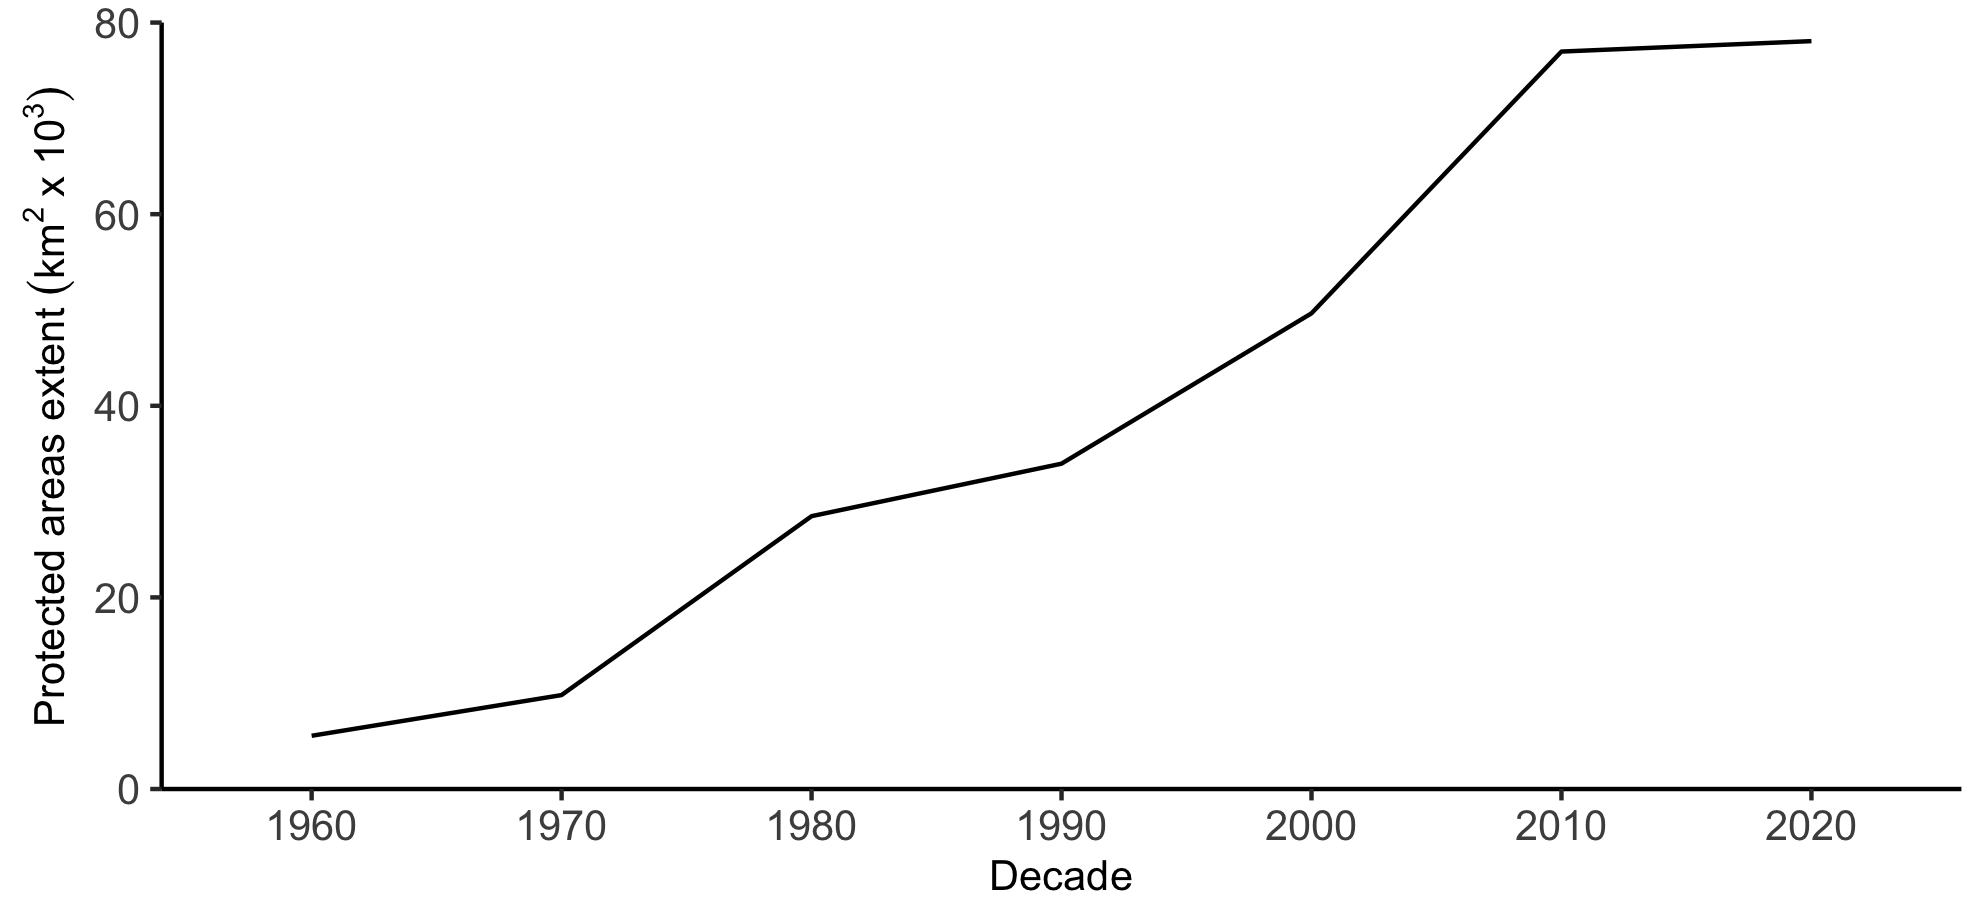
\includegraphics[width=160mm]{Fig c1-s1}
	\caption*{\small Figure S1 - Cerrado’s Strict Protection Protected Areas (PAs) area accumulation throughout time.}
\end{figure}

\subsubsection*{Figure S2}\label{fig:fig1-s2}
\begin{figure}[H]
	\centering
	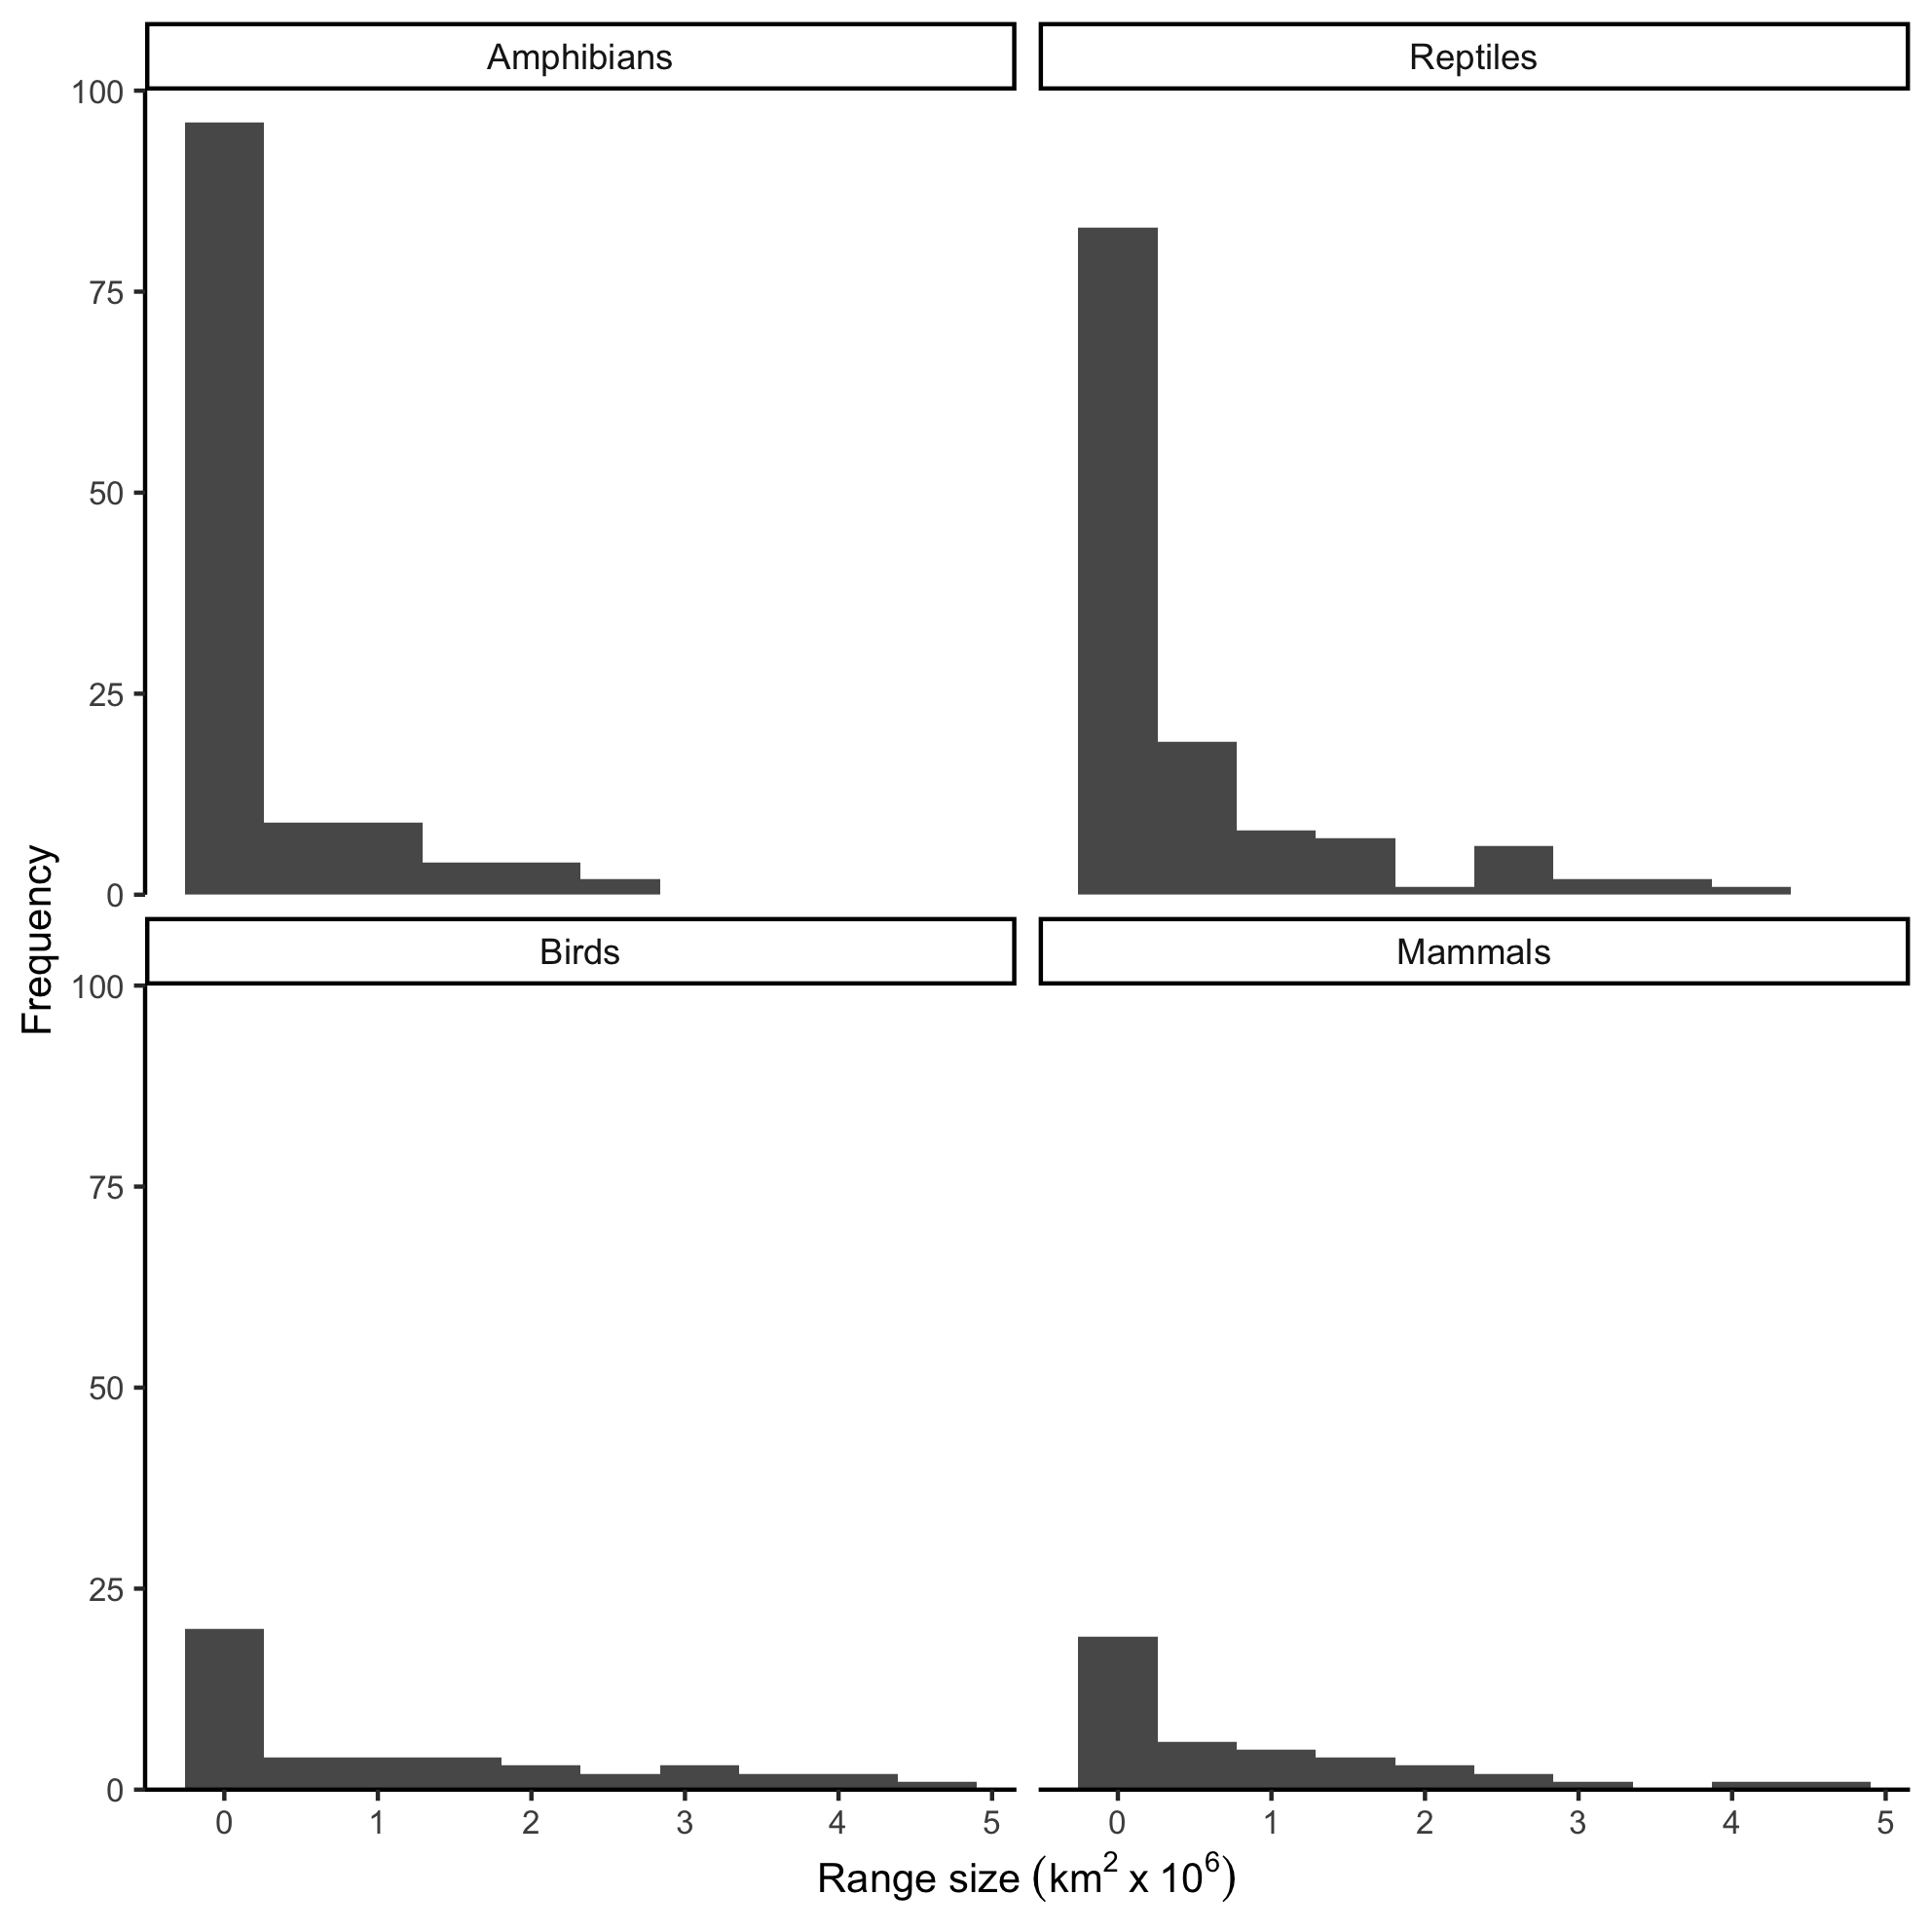
\includegraphics[width=160mm]{Fig c1-s2}
	\caption*{\small Figure S2 - Histograms of range size frequencies in each terrestrial vertebrate group}
\end{figure}

\pagebreak

\subsubsection*{Figure S3}\label{fig:fig1-s3}
\begin{figure}[H]
	\centering
	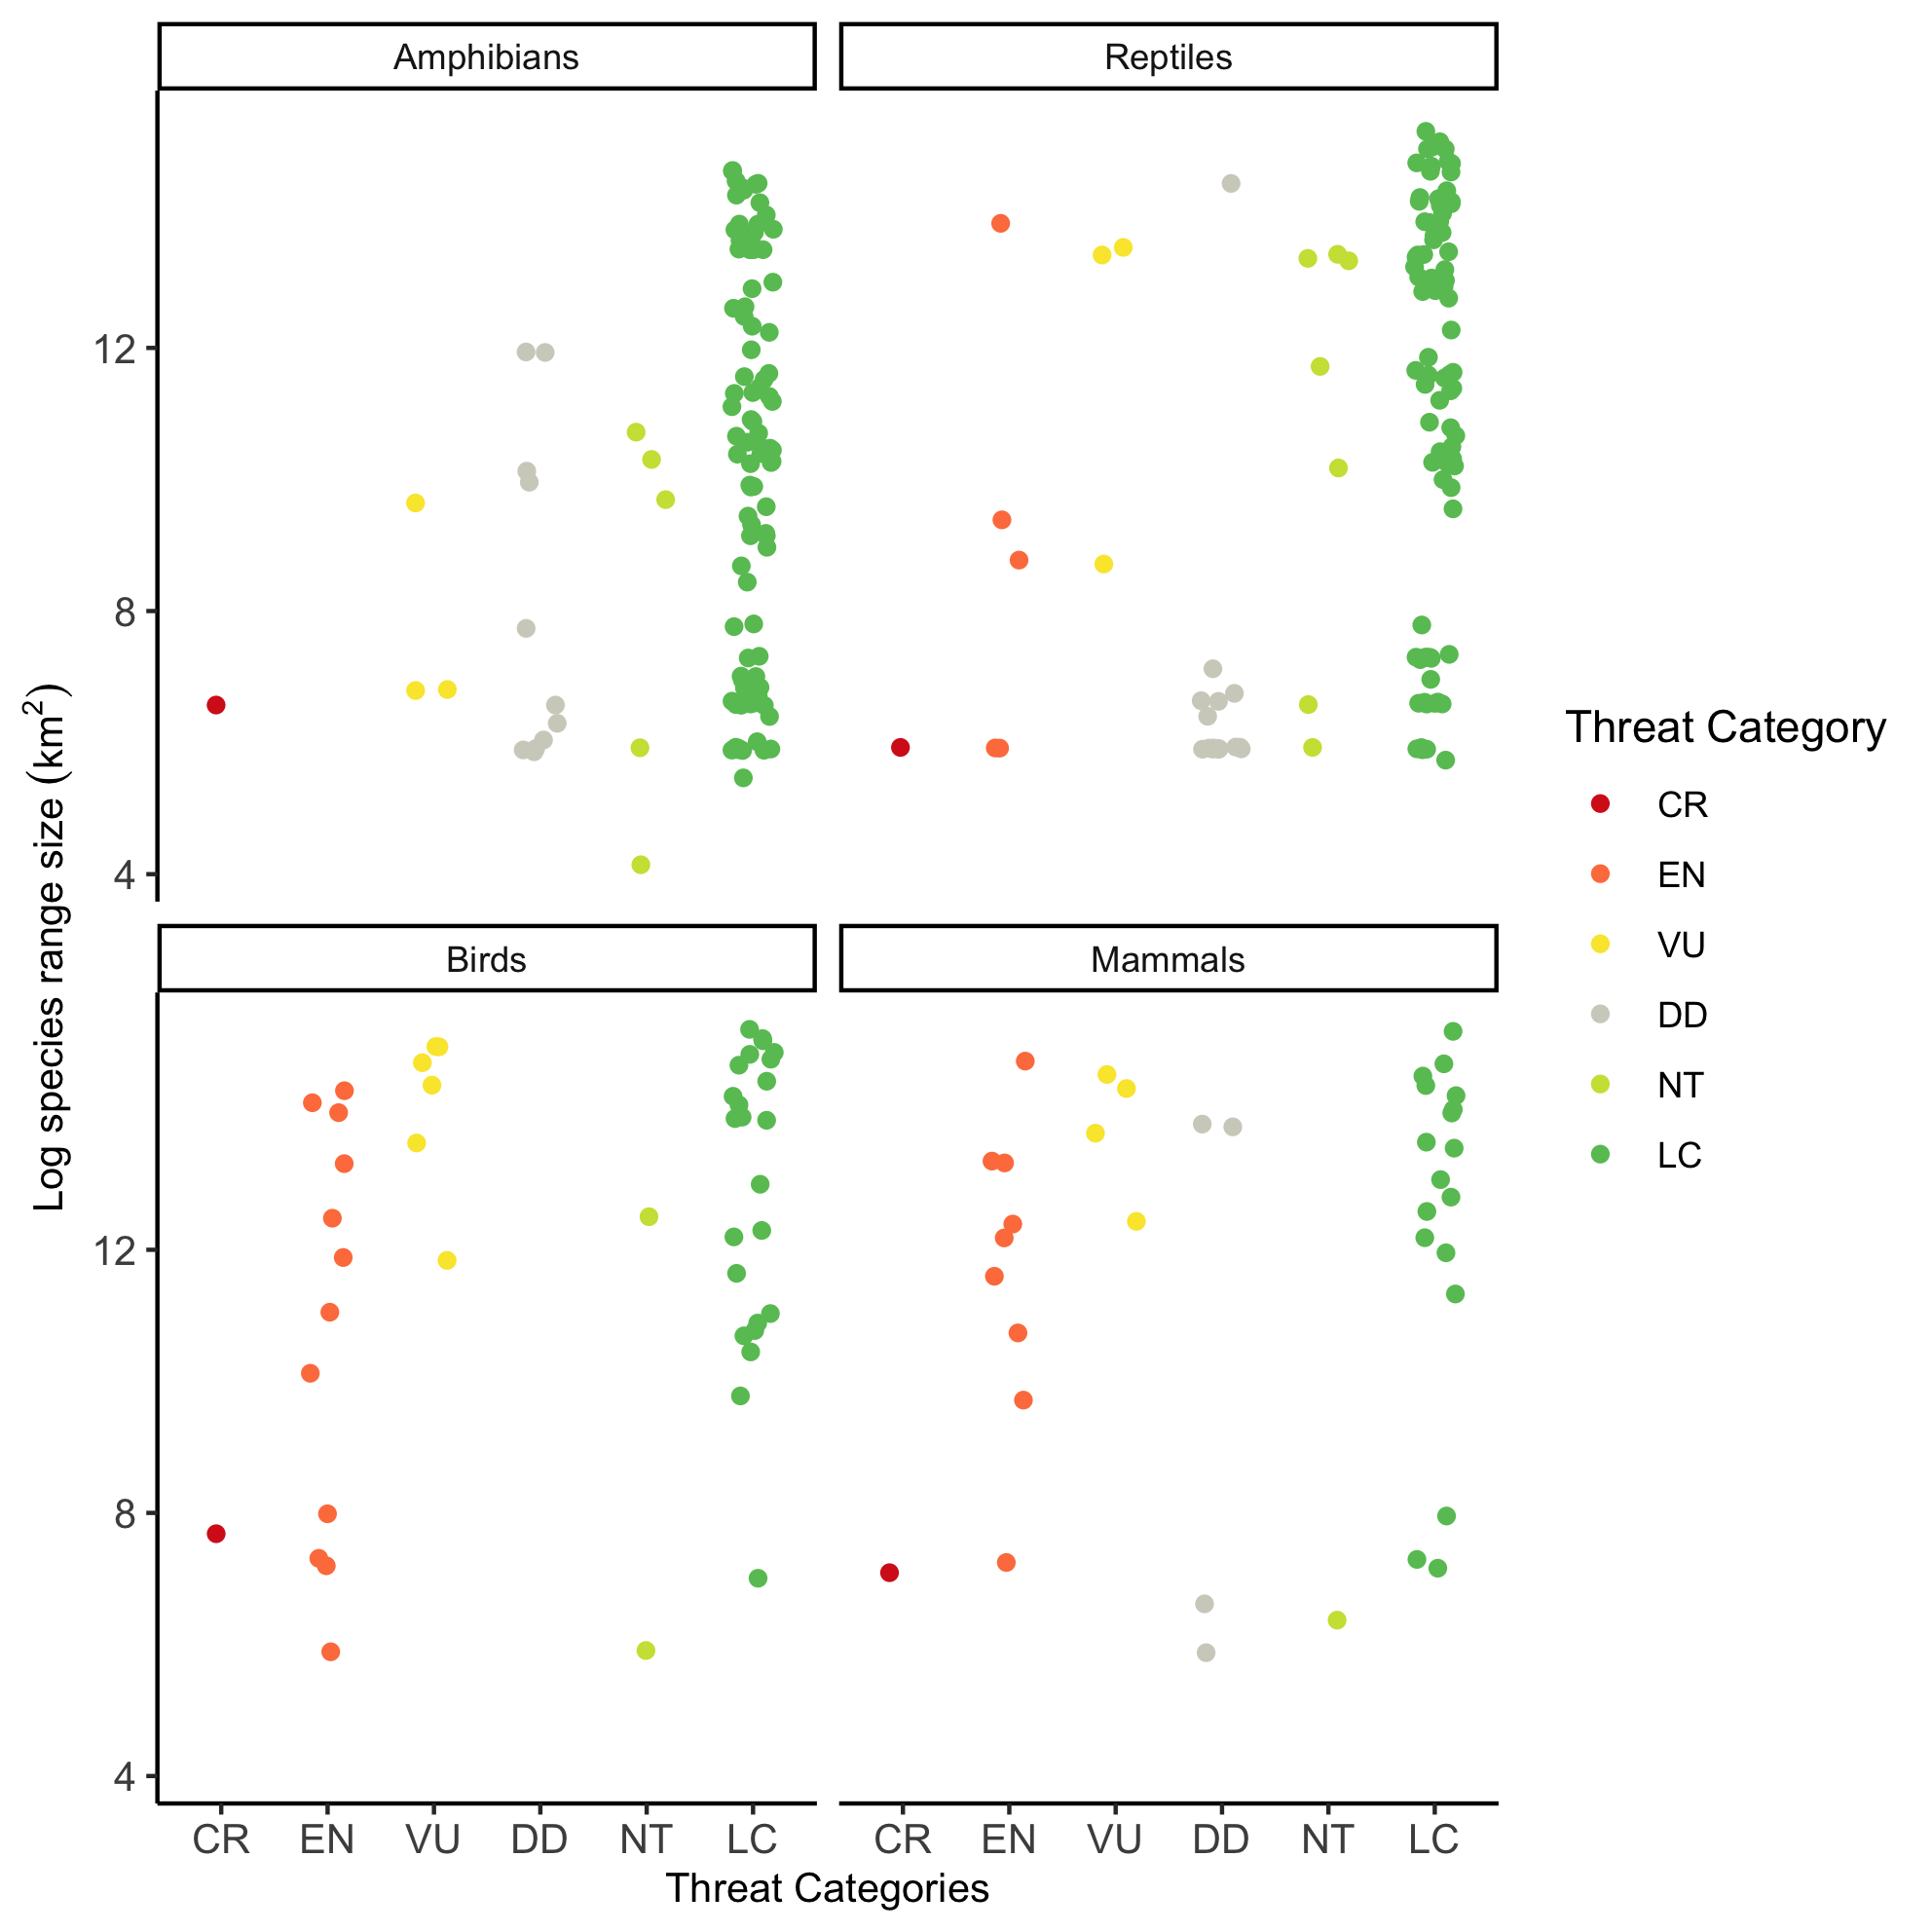
\includegraphics[width=160mm]{Fig c1-s3}
	\caption*{\small Figure S3 - Range size variation in each terrestrial vertebrate group according to ICMBio’s threat categories}
\end{figure}

\pagebreak

\subsubsection*{Figure S4}\label{fig:fig1-s4}
\begin{figure}[H]
	\centering
	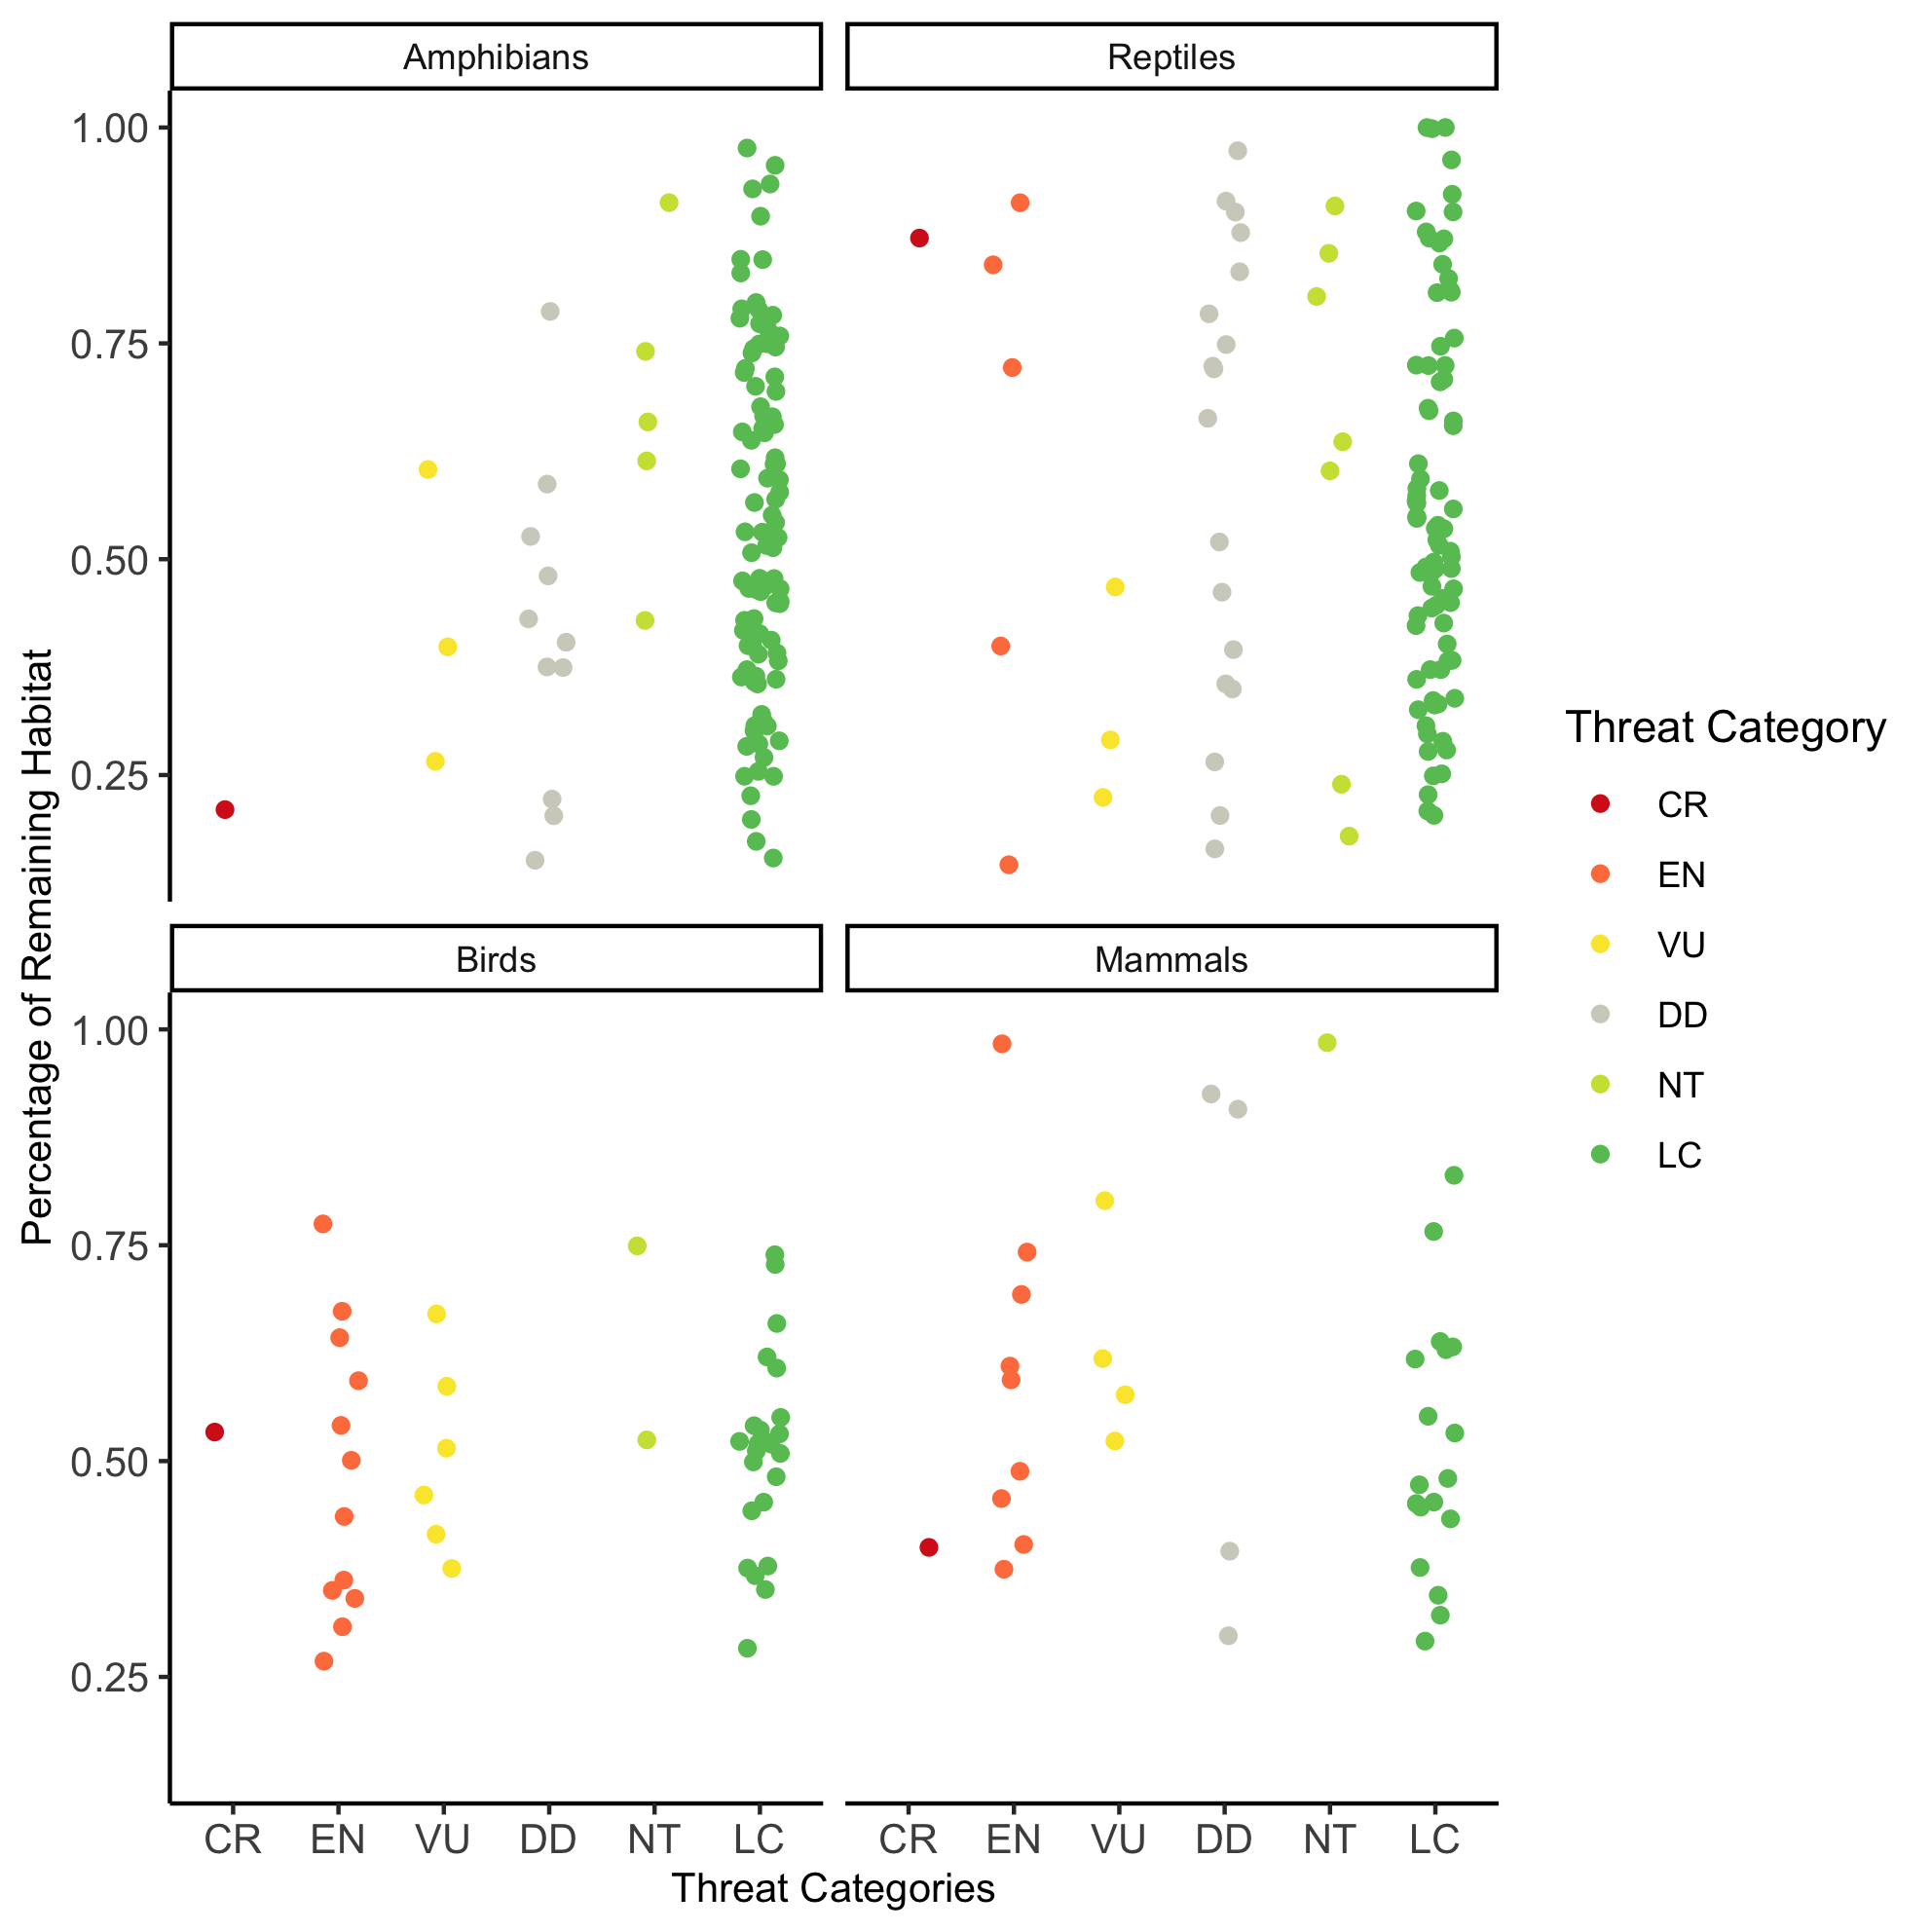
\includegraphics[width=160mm]{Fig c1-s4}
	\caption*{\small Figure S4 - Percentual habitat loss variation in each terrestrial vertebrate group according to ICMBio’s threat categories}
\end{figure}

\pagebreak

\subsubsection*{Figure S5}\label{fig:fig1-s5}
\begin{figure}[H]
	\centering
	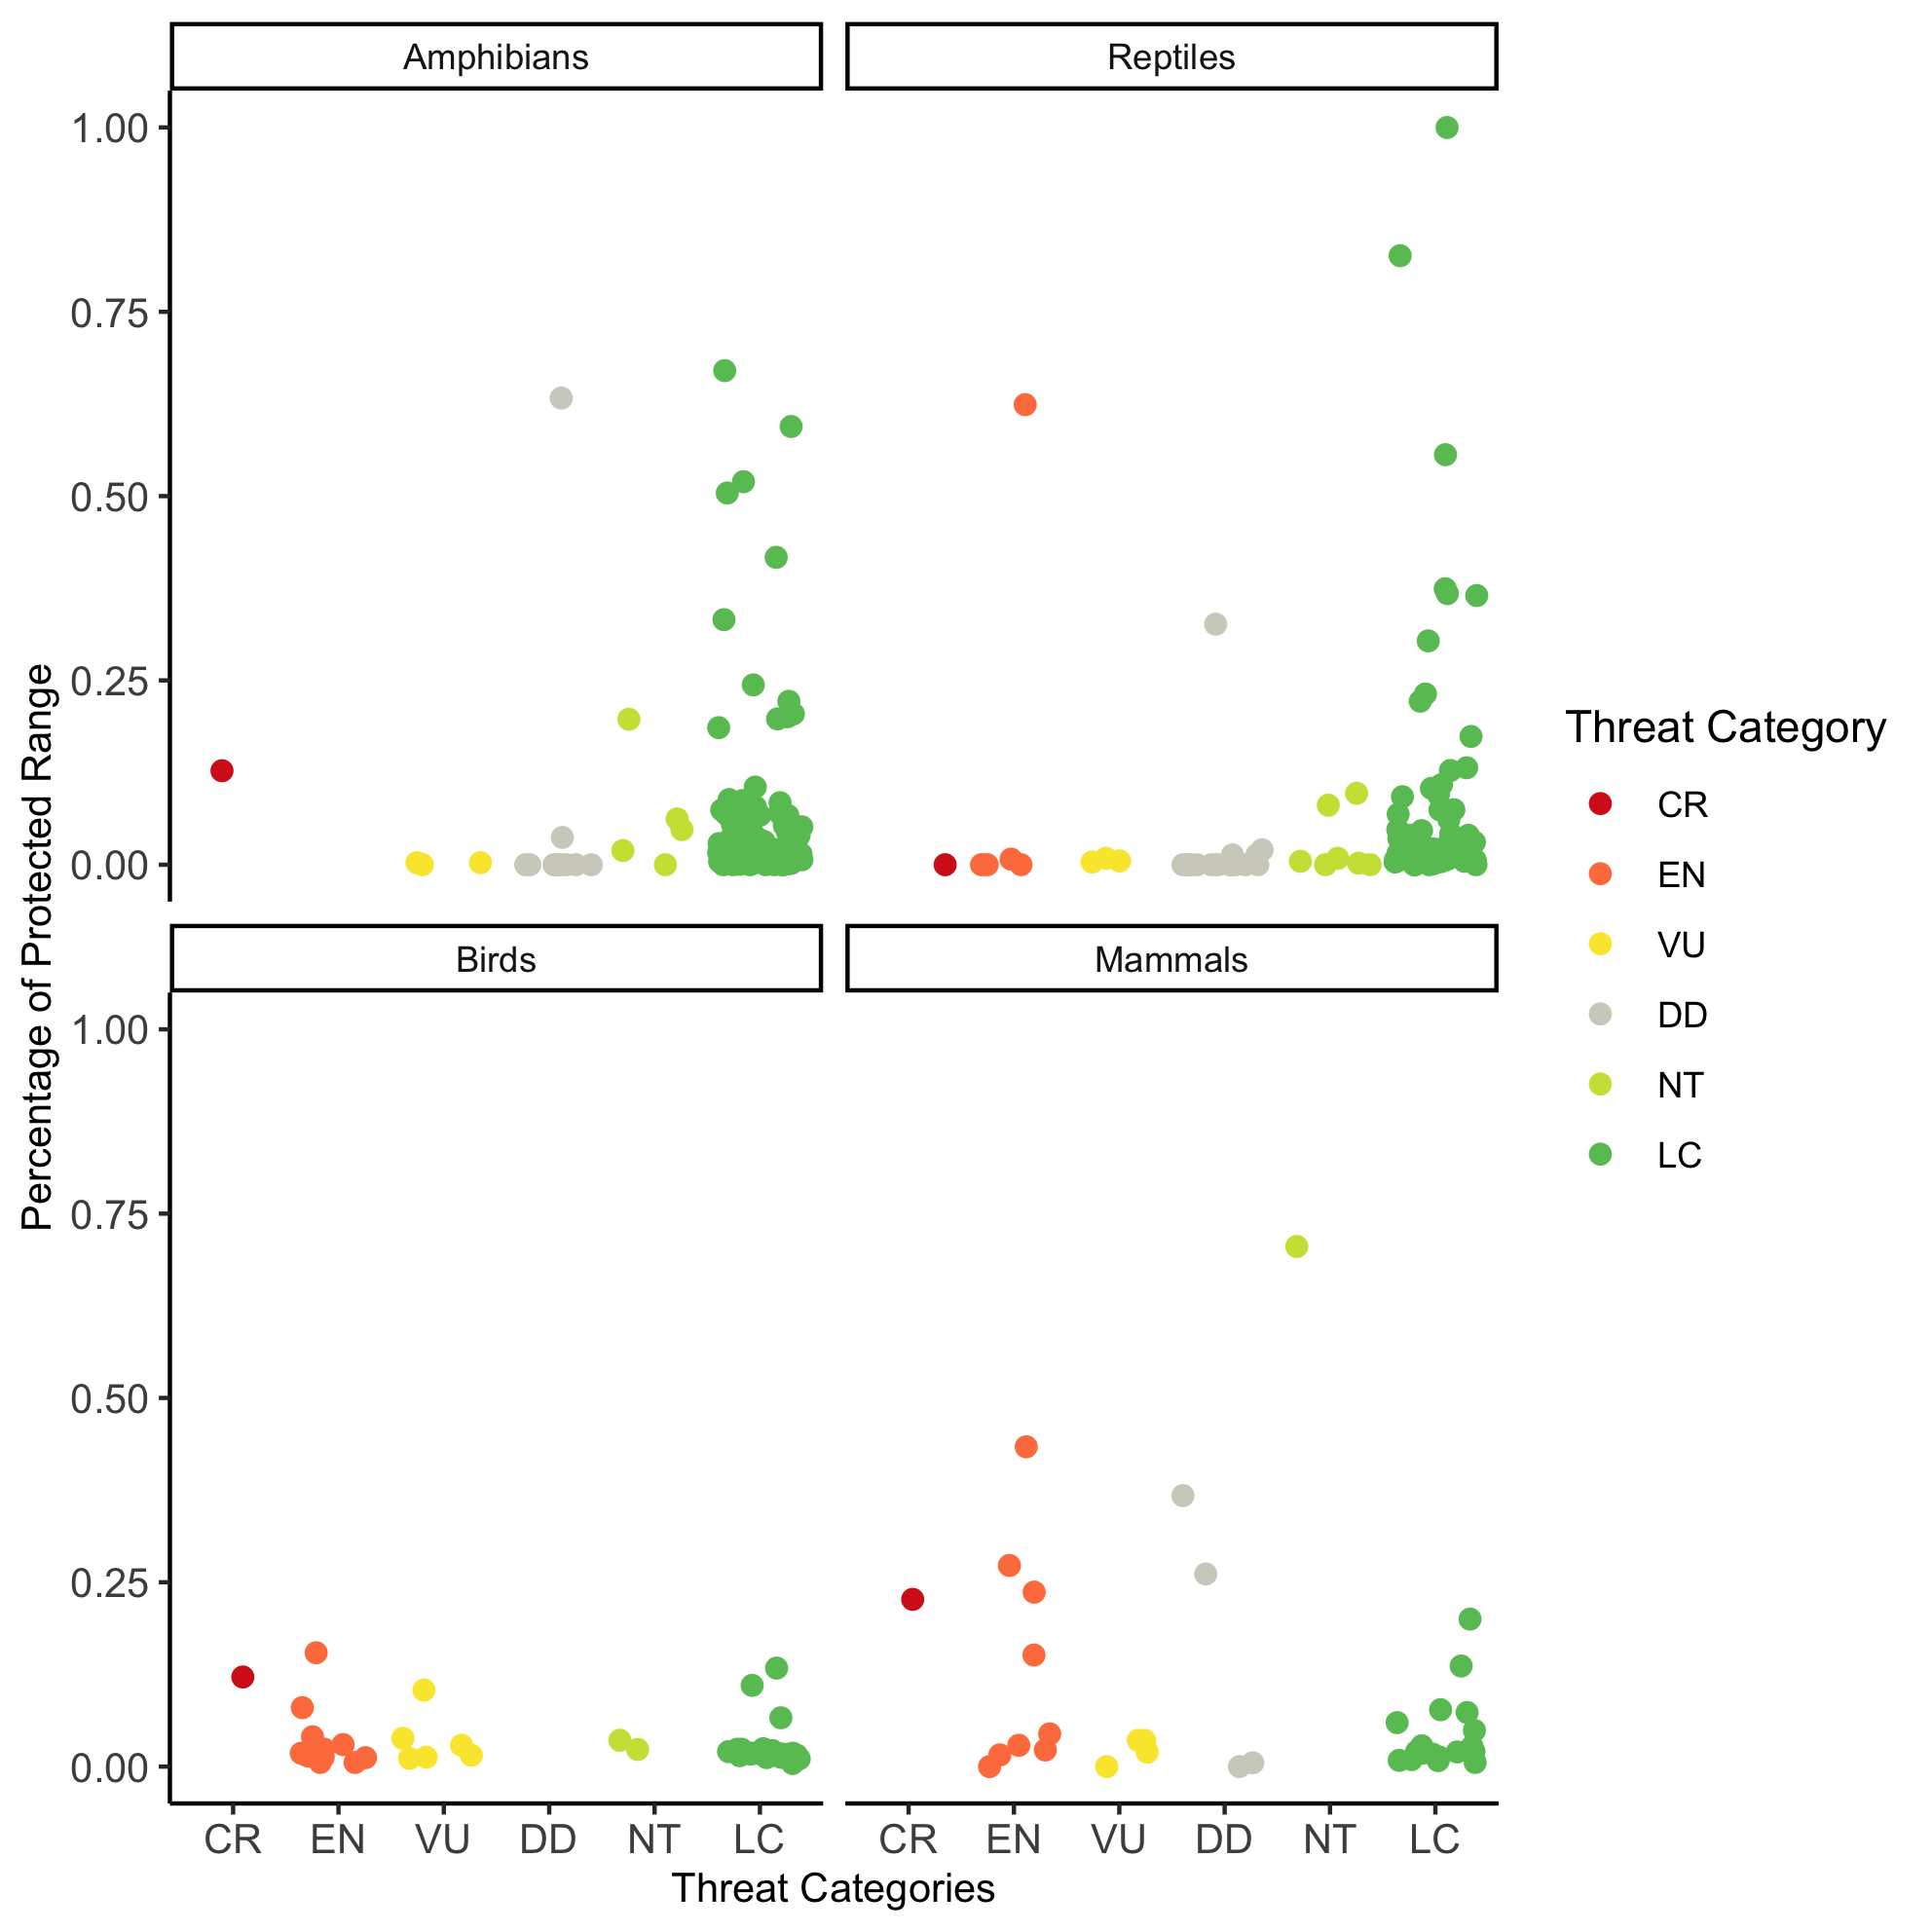
\includegraphics[width=160mm]{Fig c1-s5}
	\caption*{\small Figure S5 - Percentual protected range variation in each terrestrial vertebrate group according to ICMBio’s threat categories}
\end{figure}


%%%%%%%%%
% CAPÍTULO 2 %
%%%%%%%%%

\chapter[Cerrado endemic tetrapod bioregions]{\centering{In search of generality: revised distribution data and regionalization of Cerrado endemic tetrapods}}\label{chap2}

\begin{resumo}[\normalsize Abstract]
		\noindent
		\textbf{Aim:} To search for a general regionalization pattern using verified records of endemic terrestrial vertebrates. To test previous hypotheses of congruent distribution patterns for Cerrado biotas. To study the role of elevation as a driver of endemism and distribution in the Cerrado region.\\
		\noindent
		\textbf{Location:} Cerrado domain, central South America\\
		\noindent
		\textbf{Taxon:} Tetrapoda\\
		\noindent
		\textbf{Methods:} We used a species occurrence matrix to implement a Biotic Element analysis to test for non-random spatial congruence of raw distributions of Cerrado endemic amphibians, reptiles, birds, and mammals. We implemented multiple linear regression on elevational records of species comparing the average elevational range of all delimited Biotic Elements (BE).\\
		\noindent
		\textbf{Results:} We compiled and revised 13,800 unique distribution records of 340 Cerrado endemic tetrapods and detected a significant, non-random co-distribution pattern formed by 29 Biotic Elements comprising 182 species, and corroborating the first general prediction of the vicariant model. Most BEs were composed of at least three vertebrate groups, reflecting general tetrapod endemism patterns. Congeneric species were segregated among different BEs corroborating the second major prediction of the vicariant model. Our regionalization scheme was broadly congruent with previous results, and revealed three previously undetected areas. Most (89\%) partial or restricted BEs are clearly segregated in elevation, and we recognized 14 “Plateau units” and 12 “Depression units”.\\
		\noindent
		\textbf{Main conclusions:} Our results support an emergent consensual biotic regionalization pattern in the Cerrado. We also revealed three novel regions and complex biogeographical patterns. The clear altitudinal segregation among Biotic Elements corroborates previous ideas on the role of geomorphological changes in shaping Cerrado and Neotropical endemism patterns. Our recovered units should serve as a template for the description of new taxa, for delimiting poorly studied ranges, and for guiding urgent conservation action in the Cerrado.\\
		
		\vspace{\medskipamount}
		\noindent
		\textbf{Keywords}: Biodiversity, Bioregions, Biotic Elements, Elevation, Endemism, Tetrapods, Vicariance
\end{resumo}

\section{Introduction}\blfootnote{Essa é a segunda versão desse artigo, submetido com \textit{major revisions} ao \textit{Journal of Biogeography}. Em 05 de junho de 2023 recebemos uma segunda revisão, atualmente (18 de julho) em preparo para ressubmissão. Esse texto foi produzido com a colaboração de: Ana Paula Carmignotto, Ricardo Jannini Sawaya, Luis Fabio Silveira, Paula Hanna Valdujo e Cristiano de Campos Nogueira}

Understanding general patterns of biotic distribution is a long-standing scientific challenge (\citealp[e.g.][]{Brown1995}), and provide central empirical and theoretical elements to Evolutionary Biology, Biogeography and Biological Conservation \citep{KreftJetz2010, Holt2013, Whittaker2013}. The argument on how different areas are occupied by co-distributed biotas dates back to the eighteenth century, with the proposition of the “Buffon’s Law” by the French naturalist Georges-Louis Leclerc (“Earl of Buffon”, \citealp[see][]{Cox2016}). Key advances in the following century by \citet{Sclater1858} and \citet{Wallace1876}, proposing the first (and still largely undisputed - \citealp[see][]{Holt2013}) global map of zoogeographical realms, based on raw distribution data for birds and mammals, laid the foundation for the science known today as Biogeography \citep{Cox2016}. The validation of previous results allowed the understanding of large-scale regionalization patterns and their drivers (\citealp[see][]{Ficetola2017}).

Despite these enduring results on global Zoogeographical realms \citep{Sclater1858, Wallace1876, Holt2013}, studies of biogeographical patterns at more refined, continental scales are proportionally scarcer, with few studies aiming to test coincident distribution patterns based on data from different groups of organisms, and using quantitative, objective methods (\citealp[see][]{Holt2013, Edler2017}). This limitation results mainly from the paucity of good quality, detailed, point locality data for most organisms and in most continents \citep{Holt2013}, and is known as the Wallacean shortfall \citep{Whittaker2005}. As a result, biogeographical studies generally include data only from particular clades or groups of organisms, and general patterns based on larger taxonomic units are rarely documented and tested at continental or subcontinental scales \citep{KreftJetz2010, Holt2013}. As a consequence, regional biotic subdivisions and resulting spatial units in biogeography are often defined arbitrarily \citep{KreftJetz2010, Edler2017}.

If high-quality, reliable species distribution data is available, the difficulties related to delimiting biogeographical units should decrease when large and diverse groups of taxa are analysed \citep{Nelson1981, KreftJetz2010}. Indeed, geological processes that modify large areas should affect the geographical distribution of entire biotas, formed by different groups of organisms \citep{Wiley1988}, so that these groups will tend to share similar patterns of distribution and endemism \citep{Wiley1988, Hausdorf2002}. In the megadiverse Neotropics, however, large gaps in basic faunistic knowledge have hampered broader, comprehensive, multi-taxon analyses of endemism and biotic regionalization \citep{KreftJetz2010, Holt2013}. This lack of studies is also verified in the savannas that dominate the central portion of South America, in the biodiversity hotspot known as Cerrado, the richest and most imperilled tropical savanna in the globe \citep{Colli2020}.

Until recently, analyses on Cerrado endemism and biotic regionalization were scarce and based on limited data \citep{Colli2020}. Earlier studies described Cerrado vertebrate biotas as impoverished, poor in endemics and dominated by widespread, generalist taxa (\citealp[see][]{Vanzolini1963, Sick1965}). The first zoogeographical interpretations of the Cerrado \citep{Vanzolini1963}, based on the distribution of reptiles, proposed two major areas of endemism, a septentrional (Northeastern) and a meridional (Southwestern) portion. Later, \citet{Silva1997}, recovered four areas of endemism, based on the distributions of endemic bird species, all coincident with major topographic units in central Brazil \citep{Silva1997}. Despite centuries of scarcity of data, targeted inventories in the last three decades and recent analyses led to important advances in the understanding of the Cerrado terrestrial vertebrate fauna \citep{Nogueira2010, Carmignotto2012, Valdujo2012, Azevedo2016}. These new inventories led to the discovery and description of hundreds of new vertebrate species, many endemic to central Brazil (\citealp[see examples in][]{Nogueira2010}) and often showing localized ranges (\citealp[see trends in][]{Gaston1996}). However, drivers of distribution and endemism patterns in central Brazil are still poorly understood, and the importance of landscape evolution, climatic stability, and vicariance have just started to be acknowledged \citep{Silva1997, Lopes2008, Nogueira2011, Werneck2011, Azevedo2016, Carmignotto2022}. In this scenario of rapid data accumulation and rampant habitat loss (\citealp[see][]{Colli2020}), understanding endemism patterns at refined scales becomes even more urgent (\citealp[see][]{Brooks2006}), especially when neither biodiversity nor threats are equally distributed throughout the territory (\citealp[e.g.][]{Azevedo2016, Strassburg2017, Francoso2020}).

Recent analyses on the more extensive distributional database of endemic squamate reptiles and anurans \citep{Nogueira2011, Azevedo2016}, provided the first quantitative analyses of regionalization patterns of the Cerrado endemic fauna. The complex and novel endemism patterns revealed in these studies were largely defined by topographical divisions between large, ancient flatland plateaus and younger peripheral depressions, corroborating earlier biogeographical interpretations \citep{BrownGiff2002, Silva2002}. Additionally, elevation has been recovered as a major driver of assemblage dissimilarity in Cerrado amphibians \citep{Valdujo2013} and therefore is likely to be related to the formation of regionalized species groups. The insular condition of Cerrado plateaus is also pointed as a potential determinant of endemism in the plant genus Mimosa, that peaks in upland interfluvial savannas and grasslands of central Brazil \citep{Simon2000}. However, all these studies involved limited groups of organisms, and their conclusions may not reflect general patterns for entire biotas. Combining distributional data of all tetrapod groups should enhance the chance of detecting a general, significant biogeographical signal, resulting from large-scale historical processes that affected different groups of organisms, despite their broad ecological differences \citep{Roll2017}.

We aimed herein to (1) test previous hypotheses of congruent distributional patterns in the Cerrado based on the first revised and updated distributional dataset including all known Cerrado endemic tetrapods; (2) test the role of elevation (plateaus x depressions) as a potential driver of Cerrado terrestrial vertebrate endemism; and (3) propose a robust, objective and general biogeographical regionalization scheme for the richest and most endangered tropical savanna on the planet, supported by a large, revised point-locality database for tetrapods, one of the best studied groups of organisms (\citealp[see][]{Gaston1996, Roll2017}).

\section{Materials and Methods}
\subsection{\textit{Study area}}

The Cerrado is the largest savanna in the Neotropics, and occupies a central position in South America, along ancient uplands of the Brazilian shield, separating lowland open areas of the Caatinga in the northeast from the Chaco in the southwest, and also dividing Amazonian in the northwest from the Atlantic Forest in the southeast. The Cerrado vegetation is dominated by upland savannas and grasslands, along extensive ancient plateaus, intermingled by peripheral, mostly forested depressions, associated with upper portions of major drainages of South America (Tocantins-Araguaia, Paraná, Paraguay, Guaporé, and São Francisco, \citet{Absaber1998}). These topographical and edaphic conditions generate a complex landscape mosaic of grassland and savanna, crossed by palm marshes and gallery forests along drainages \citep{Eiten1972, Ratter1997}, a pattern observed both at local and continental scales, forming complex, horizontally stratified landscapes \citep{Silva2002, Colli2020}.

Despite being considered a global biodiversity hotspot \citep{Myers2000} the region is still poorly protected and remains under strong pressure from the expansion of agricultural activities \citep{Strassburg2017, Grande2020, Pacheco2021}. Of the approximately 200 million hectares covered by Cerrado, only 19.8\% remain intact and only 7.5\% are legally protected. Meanwhile, recent (2002-2011) rates of deforestation were 2.5 times higher than in Amazonia \citep{Strassburg2017}.

\subsection{\textit{Data sources}}

Our database was built based on three major sources: 1 - standardized field surveys planned to fill previous sampling gaps in the Cerrado (\citealp[see][]{Nogueira2009, Valdujo2012, Carmignotto2022}), 2 - broad revision of vouchered specimens deposited in major scientific collections, and 3 - compilation of reliable records in the taxonomic literature (\citealp[details in][]{Nogueira2009, Valdujo2012, Nogueira2019, Carmignotto2022}). We did not include records from online digitized biodiversity data (such as GBIF or similar electronic databases, that often comprise error-prone, raw data, \citealp[see][and references therein]{Nogueira2019}).

We updated the list of Cerrado endemic terrestrial vertebrate species presented in previous studies \citep{Silva1997, Nogueira2011, Carmignotto2012, Azevedo2016, GutierrezMarinho2017}, and used only verified point-locality records to map geographical ranges of Cerrado endemic terrestrial vertebrate species (listed in \nameref{sup:2-s1} in \nameref{sec:supinfo-2}). We considered as endemic those species whose ranges are fully or largely coincident with the approximate limits of the Cerrado provided in \citeauthor{Dinerstein2017} (\citeyear{Dinerstein2017}, \citealp[see also][]{IBGE1993, Olson2001}). Species with marginal records in transitional areas between the Cerrado and other domains, but with local ranges associated with typical Cerrado habitats, were also considered endemic, due to their possible historical association to once continuous savannas (currently isolated as disjunct areas).

The taxonomy follows specific literature for each vertebrate group (\citealp{Frost2020} for amphibians, \citealp{Uetz2020} for lizards/amphisbaenians, \citealp{Nogueira2019} for snakes, \citealp{Pacheco2021birds} for birds, and \citealp{Abreu2021} for mammals). We included in our analyses species described up to early January 2021.


\subsection{\textit{Analyses}}

We obtained a presence-absence matrix via the intersection of revised point-locality records and 244 1º x 1º grid cells covering the Cerrado \citep{Dinerstein2017}. We used the same grid size and position (grid origin) as in \citet{Azevedo2016}, to make results more comparable. Subsequently, we created a dissimilarity matrix based on the presence-absence matrix using the geco coefficient. As in \citet{Azevedo2016}, we found our 1º x 1º grid relatively coarse compared to our point-locality dataset and therefore we set the required geco tuning constant to \textit{f} = 0.2 (\citealp[see][]{Hennig2006} for a more detailed explanation about the geco coefficient).

We then used this matrix to implement a Biotic Element analysis in ‘prabclus’ \citep{Hausdorf2003, Hennig2020}, an add-on package for the statistical software R (available at \url{http://cran.r-project.org}). This analysis provides a test for the first major prediction of the vicariance model: non-random congruence of species ranges as a result of allopatric speciation, caused by the emergence of biogeographical barriers \citep{Hausdorf2006}. Therefore, we should be able to detect groups of species whose ranges are more similar to each other than to ranges of species assigned to other such groups, even in the presence of limited dispersal and peripheral sympatry \citep{Hausdorf2002, Hausdorf2003}. To do so, we compared the geographical ranges using the function \textit{‘prabtest’} which is a parametric bootstrap test for the non-random congruence of species distributions. Null models were generated producing artificial ranges based on parameters (richness per cell, range size distributions, and patterns of spatial correlation and disjunction) obtained from the original dataset \citep{Hennig2004}. The test statistic \textit{T} derives from the assumption that if clusters of ranges are present in the dataset, geographical distances among clustered ranges should be smaller than distances between ranges simulated at random. This statistic is calculated as the ratio between the 25\% smallest and the 25\% largest distances, and it is expected to be smaller than expected by chance if ranges are clustered, and larger for homogeneous, non-regionalized data \citep{Hennig2004}. Then, the distribution of the statistical test under null models was approximated by Monte Carlo simulation (1,000 replicates).

According to the second major prediction of the vicariance model, closely related species should be distributed among different biogeographical units, as an effect of biogeographical barriers and the fragmentation of ancestral ranges followed by speciation \citep{Wiley1988, Hausdorf2003, Hausdorf2006}. To verify if species of the same genus were segregated among different Biotic Elements (hereafter “BEs”), we implemented a chi-square test in ‘prabclus’ (function \textit{‘comp.test’}; \citealp[][]{Hennig2020}). If a non-significant result is found, i. e. closely related species are not clustered in the same BEs, then the second major prediction of vicariance is corroborated, with evidence of lineage fragmentation across different areas.

In addition to the test of vicariant predictions via Biotic Element analysis, we examined if species predominantly occurring in plateaus or depressions were scattered among different BEs or clustered in the same units. To do so, we also implemented a chi-square test in ‘prabclus’ (function \textit{‘comp.test’}; \citealp[][]{Hennig2020}). A significant result, i.e. BEs formed predominantly by species from the same altitudinal compartment (plateau/depression), indicates elevation as a putative driver of isolation among endemic Cerrado biotas. To classify species as typical of plateaus or depressions we compared elevation records to a random sample of 1000 records in the Cerrado, using a Kruskal-Wallis test (\citealp[see][for similar analyses]{Nogueira2011}). Species with significant results and showing median elevation value above or below 500 m (\citealp[see][]{Silva1997}) were classified as plateau or depression species, respectively. Species with non-significant results but with 75\% of records (defined by the limit of the 1st or 3rd quartile) above or below the 500 m were classified as plateau or depression species, respectively. The remaining species were classified as showing a general altitudinal range. Similarly, BEs were also classified as plateau, depression or general according to these same criteria.

\subsection{\textit{Mapping}}

We clustered species ranges using the hierarchical method (function \textit{‘hprabclust’}) in ‘prabclus’. This method clusters distributions by taking the h-cut partition of hierarchical clustering and declaring all members of too small clusters as noise. This gives a distance-based clustering method, which estimates the number of clusters and allows for noise/non-clustered ranges \citep{Hennig2020}. The function \textit{‘hprabclust’} requires two main parameters: a) the \textit{cutdist} - a value of the h-cut partition, and b) the \textit{nnout} - the minimum number of species demanded to recognize a cluster. Smaller \textit{nnout} values allow the detection of higher numbers of BEs by recognizing clusters with at least two species (when \textit{nnout} = 1, i. e. the smallest possible composition of an area of endemism, \citealp[][]{Hausdorf2002}) while assigning fewer species to the noise component. However, as the number of species in a dataset increases, we should expect an increased number of species in the noise component (from the formula \textit{k} = number of species/40, used in \citealp[][]{Hausdorf2003}, where \textit{k} is a constant that represents an initial estimate of noise, \citealp[see][for detailed explanations]{Byers1998}). Therefore, to reduce as much subjectivity as possible in the choice of these clustering parameters, we compared combinations of \textit{cutdist} between 0.10 and 0.50 (dissimilarity values within clusters) by increases of 0.05, and \textit{nnout} between one and five (two to six species to recognize a cluster), and only pre-visualized cluster outcomes where the proportion of ‘Noise/Number of BEs’ was near the estimated \textit{k} value (8.5 in the present study; see \nameref{sup:2-s2} in \nameref{sec:supinfo-2}). We regard this as a conservative approach in the detection of BEs by hierarchical clustering.

To optimize parameter comparisons, we used the function \textit{‘cdn’} from the package ‘mapar’ \citep{VieiraAlencar2022}. To check the spatial contiguity of units for each relevant \textit{cutdist-nnout} combination, we pre-visualized the resulting BEs, as well as their component species and percentage of species per grid cell, using the \textit{‘mapar’} function, also from the ‘mapar’ package, in R environment. Finally, to illustrate detected units we chose a combination of \textit{cutdist} and \textit{nnout} that maximized dissimilarity between BEs while preserving spatial contiguity within units.

Following \citet{Nogueira2019}, we classified species ranges as “restricted”, “partial” or “widespread” based on their extent in relation to the study region (see \nameref{sup:2-s1}). Restricted range species are those with known records concentrated in a relatively small geographical area (typically smaller than 50,000 km\textsuperscript{2}, \citealp[see][]{Eken2004}); partially distributed species are those recorded only at a given portion of the study region (typically up to half of the entire region); and widespread species are those recorded in most or all of the study region. Then, for the purpose of description, we classified BEs according to the most common category of ranges among their component species.

We mapped the detected Biotic Elements selecting the group of grid cells that contained at least one record of its component species. Grid cells with more than 70\% of component species were considered “core cells”, while grid cells with more than 30\% and up to 70\% of component species were “intermediate cells”. Finally, grid cells with less than 30\% of component species were considered “marginal cells”.

\section{Results}
\subsection{\textit{Species distribution dataset}}

Our verified point-locality database includes 340 taxa, comprising 124 amphibians, 129 reptiles, 45 birds, and 42 mammals, and an updated list of Cerrado endemic terrestrial vertebrate species, including a synthesis of range data, is provided in \nameref{sup:2-s1}. The addition of mammals and birds, as well as the inclusion of amphibians and squamates described after \citet{Azevedo2016}, added a total of 9,416 new records to our analyses, totalling 13,800 unique records. To our knowledge, our point-locality database represents the most reliable, detailed and comprehensive compilation of endemic vertebrate distribution in the Cerrado. The grid system and the resulting presence-absence matrix are available in \nameref{sup:2-s3} and \nameref{sup:2-s4}, respectively.

\subsection{\textit{First prediction of the vicariance model: test for clustered ranges}}

The observed T statistic (0.3065) was significantly smaller than expected by chance (\textit{T} varied between 0.3165 and 0.3693, with a mean of 0.3448 in 1,000 artificial populations generated under null models; \textit{p} < 0.001). This indicates that ranges of endemic terrestrial vertebrates form distinguishable, non-random, regionalized biotas in the Cerrado, corroborating the first major prediction of the vicariance model and detecting a significant regionalization pattern for Cerrado endemic terrestrial vertebrates \citep{Hausdorf2003, Hennig2004, Hausdorf2006}.

\subsection{\textit{Identification of Biotic Elements}}

In the clustering analysis, 182 species (ca. 53\% of the total) were assigned to 29 Biotic Elements (\autoref{tab:tab2-1}), with 158 species (ca. 46\%) included in the noise component. The combination of \textit{cutdist} = 0.15 and \textit{nnout} = 2 preserved spatial contiguity while increasing the number of BEs and producing a proportion “Noise/Number of BEs” around five, while requiring at least three co-distributed species to recognize a cluster. Although other combinations resulted in proportions closer to 8.5 (see \nameref{sup:2-s2}), the inclusion of species with wider distributions frequently contributed to the detection of poorly delimited units.

\begin{table}
	\centering
	\caption[Biotic Elements (BEs categories and composition)]{\small Range size and elevational category, total number of species, and number of species per vertebrate group within BEs. Asterisks indicate BEs detected for the first time in the Cerrado.}
	\label{tab:tab2-1}
	\vspace{\bigskipamount}
	\footnotesize
	\begin{tabular}{c c c c c c c c c c c c}
		\hline
		\textbf{BE} & \textbf{Range size} & \textbf{Elevation} & \textbf{Total} & \textbf{W} & \textbf{P} & \textbf{R} & \textbf{Amphibians} & \textbf{Reptiles} & \textbf{Birds} & \textbf{Mammals}\\
		\hline
		1 & restricted & plateau & 39 & 0 & 3 & 36 & 21 & 9 & 5 & 4\\
		2 & wide & general & 17 & 14 & 3 & 0 & 3 & 2 & 11 & 1\\
		3 & restricted & plateau & 13 & 0 & 0 & 13 & 10 & 1 & 0 & 2\\
		4 & partial & plateau & 10 & 0 & 10 & 0 & 1 & 5 & 4 & 0\\
		5 & restricted & plateau & 8 & 0 & 1 & 7 & 6 & 2 & 0 & 0\\
		6 & restricted & depression & 7 & 0 & 0 & 7 & 3 & 3 & 0 & 1\\
		7 & restricted & plateau & 7 & 0 & 0 & 7 & 2 & 5 & 0 & 0\\
		8 & restricted & plateau & 6 & 0 & 0 & 6 & 5 & 1 & 0 & 0\\
		9 & restricted & plateau & 6 & 0 & 2 & 4 & 4 & 1 & 0 & 1\\
		10 & restricted & depression & 5 & 0 & 0 & 5 & 1 & 4 & 0 & 0\\
		11 & restricted & depression & 5 & 0 & 2 & 3 & 0 & 2 & 1 & 2\\
		12 & restricted & plateau & 4 & 0 & 0 & 4 & 3 & 1 & 0 & 0\\
		13 & partial & plateau & 4 & 0 & 4 & 0 & 2 & 0 & 2 & 0\\
		14 & partial & plateau & 4 & 0 & 4 & 0 & 0 & 4 & 0 & 0\\
		15 & partial & depression & 4 & 0 & 3 & 1 & 1 & 0 & 2 & 1\\
		16 & restricted & plateau & 4 & 0 & 0 & 4 & 1 & 3 & 0 & 0\\
		17 & restricted & depression & 3 & 0 & 0 & 3 & 0 & 3 & 0 & 0\\
		18 & restricted & plateau & 3 & 0 & 0 & 3 & 0 & 3 & 0 & 0\\
		19* & restricted & depression & 3 & 0 & 1 & 2 & 2 & 0 & 0 & 1\\
		20 & restricted & depression & 3 & 0 & 0 & 3 & 1 & 2 & 0 & 0\\
		21 & restricted & plateau & 3 & 0 & 1 & 2 & 2 & 0 & 1 & 0\\
		22 & partial & general & 3 & 0 & 3 & 0 & 1 & 2 & 0 & 0\\
		23 & partial & depression & 3 & 0 & 3 & 0 & 1 & 2 & 0 & 0\\
		24* & restricted & plateau & 3 & 0 & 0 & 3 & 2 & 0 & 0 & 1\\
		25 & restricted & general & 3 & 0 & 0 & 3 & 0 & 3 & 0 & 0\\
		26 & partial & depression & 3 & 0 & 2 & 1 & 2 & 0 & 1 & 0\\
		27* & restricted & depression & 3 & 0 & 1 & 2 & 0 & 2 & 0 & 1\\
		28 & partial & depression & 3 & 0 & 2 & 1 & 3 & 0 & 0 & 0\\
		29 & partial & depression & 3 & 1 & 2 & 0 & 1 & 2 & 0 & 0\\
		\hline
	\end{tabular}

W, P and R= number of widespread, partially distributed and restricted-range species, respectively.
\end{table}
Biotic Elements were named according to the position of their core cells in relation to major topographic units, as in \citet{Nogueira2011} and \citet{Azevedo2016}. No BE was formed exclusively by a single vertebrate group (\autoref{tab:tab2-1}). Numbers of species from each terrestrial vertebrate group assigned to BEs and the noise component were not significantly different from the total of analyzed species in each vertebrate group ($\chi^2$= 20, \textit{df} = 16 \textit{p} = 0.2202). In other words, all terrestrial vertebrate groups are proportionally prone to be assigned to the noise component or to BEs, independent of the number of species per group. 

According to the predominant range size category among species in each BE, 19 units were composed mostly of restricted-range species (\autoref{fig:fig2-1}, see also \autoref{tab:tab2-1}). Only one unit was composed primarily of wide ranging species and was classified as a widespread unit (\autoref{fig:fig2-2}a), with nine units composed mostly of partially-distributed species (\autoref{fig:fig2-2}b-f). The list of species within each BE described above as well as in BEs detected in previous analysis can be found as \nameref{sec:supinfo-2} (see \nameref{sup:2-s1}).

\subsubsection{\textit{Restricted Biotic Elements}}

Most (19, 65.5\%) of our BEs were geographically confined, and formed by restricted-range species. A total of 128 species, including all tetrapod groups, were assigned to these smaller units, composed mainly by amphibians (63 species), followed by reptiles (45), mammals (13) and birds (7) (\autoref{tab:tab2-2}). Only seven BEs had at least one partially ranged species, with a maximum of three assigned to BE 1, composed of all groups of terrestrial vertebrates (\autoref{tab:tab2-1}). BE 1 was the richest unit in our analysis, with 39 species and, among restricted BEs, was followed by BE 3 (13 species) and BE 5 (8 species). Despite the high number of species in these units, 42\% of the restricted BEs were composed of only three species (\autoref{tab:tab2-1}), indicating that restricted ranges in the Cerrado are largely allopatric.

Restricted BEs were recovered throughout the Cerrado (\autoref{fig:fig2-1}), with six units found in the western portion of the region (BEs 6, 10, 11, 19, 25 and 27). Three units were concentrated on the Central Brazilian Plateau (BEs 3, 5, and 9); three in the eastern Cerrado (BEs 7, 16 and 18) and three in the southern Cerrado (BEs 8, 21 and 24). The northern portion of the region had two restricted BEs (17 and 20), and the southeastern and central western portions had one unit each. Despite some overlap at marginal and intermediate cells, most restricted BEs showed allopatric cores, except for BEs 5 and 9 which shared a core cell at the “Chapada dos Veadeiros” plateau (\autoref{fig:fig2-1}). Additionally, except for the disjunct BE 9 (\autoref{fig:fig2-1}b), all restricted BEs presented a continuous set of core cells.

\subsubsection{\textit{Partial Biotic Elements}}

Nine (31\%) of our range clusters comprised partial BEs, composed of 37 species (\autoref{tab:tab2-1}; \autoref{fig:fig2-2}b-f). Three of these units were complementary, representing different portions of the Araguaia River basin (BEs 15, 26 and 28), while two other units shared core cells in the Upper Paraná (La Plata) basin, representing both the Southern Cerrado as a whole and the Paulistânia subregion (BEs 4 and 14 respectively). Three of the remaining units represented distinct regional portions of the Cerrado, namely: the Southeastern region (BE 13), with core cells in both the Central Brazilian Plateau and the Espinhaço range; the Tocantins basin (BE 22); and the uplands surrounding the Pantanal (BE 23). Finally, the last partial unit (BE 29) had core cells scattered from the lower Tocantins river to the western portion of the Cerrado. Partial BEs varied in terms of vertebrate composition, with reptiles and amphibians representing more than half of their component species (12 species each), followed by birds, (9 species). Most partial BEs were composed of at least two terrestrial vertebrate groups (\autoref{tab:tab2-1}).

\begin{table}[h]
	\centering
	\caption[Terrestrial vertebrate classes proportion in Biotic Elements (BEs) range-size categories]{\small Absolute number and approximate percentages of species composing BEs in each range-size category. Percentages are relative to the total number of species of a given group assigned to BEs. In parenthesis is the number of units per category.}
	\label{tab:tab2-2}
	\vspace{\bigskipamount}
	\footnotesize
	\begin{tabular}{c c c c c c c}
		\hline
		& Total & Amphibians & Reptiles  & Birds & Mammals\\
		\hline
		Widespread & 17 - 10\% (1) & 3 - 4\% (1)  & 2 - 3\% (1) & 11 - 41\% (1) & 1 - 7\% (1)\\
		Partial & 37 - 20\% (9) & 12 - 15\% (8) & 15 - 24\% (5)  & 9 - 33\% (4) & 1 - 7\% (1)\\
		Restricted & 128 - 70\% (19) & 63 - 81\% (14) & 45 - 73\% (16) & 7 - 26\% (3) & 13 - 87\% (8)\\
		\hline
	\end{tabular}
\end{table}

\begin{figure}[H]
	\centering
	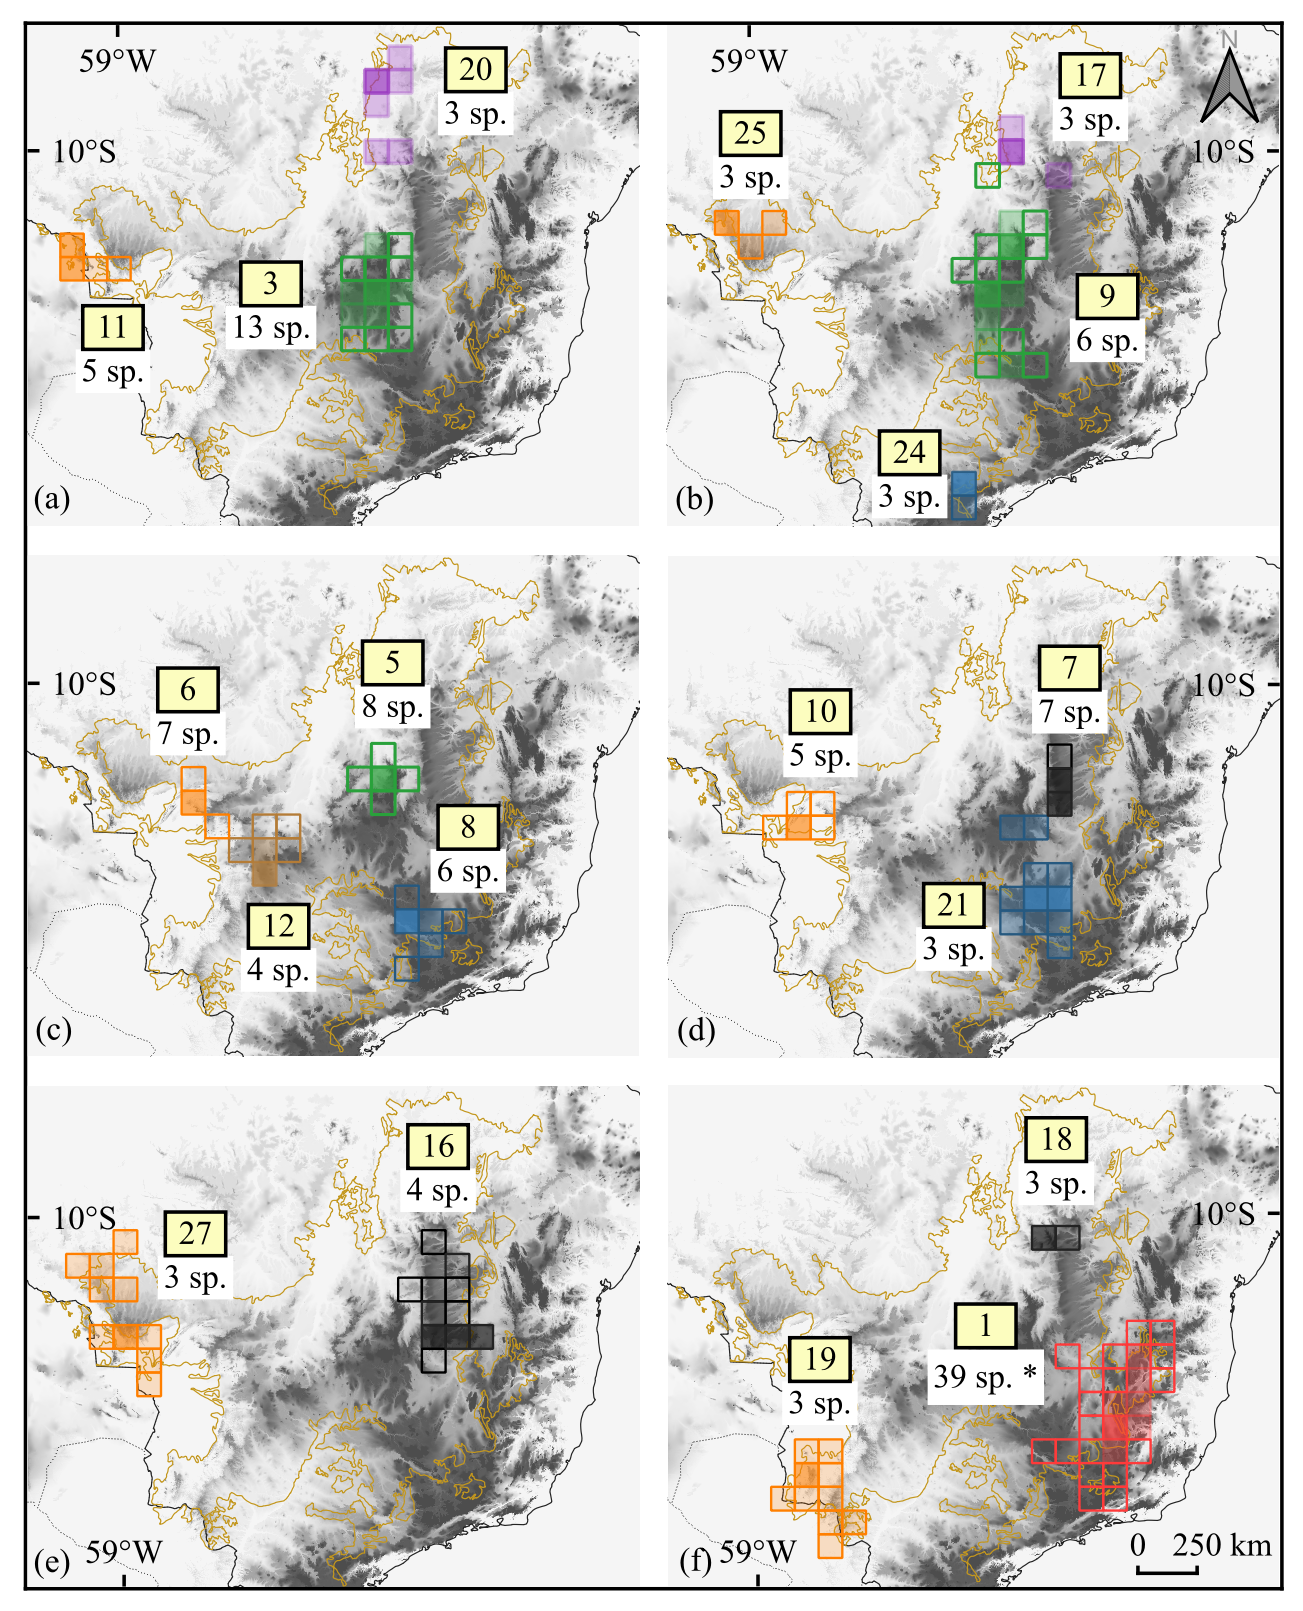
\includegraphics[width=150mm]{Fig c2-1}
	\caption[Restricted-range Biotic Elements (BEs)]{\footnotesize Restricted-range Biotic Elements (BEs) composed of endemic terrestrial vertebrates in the Cerrado (limits represented by the yellow line). BEs named according to major topographic units or as in \citet{Azevedo2016} for BEs composed of at least 50\% of the same species in both studies: (a) 3 - Central Brazilian plateau - Brasília nucleus; 11 - Huanchaca plateau/Guaporé River valley; 20 - Lower Tocantins River valley. (b) 9 - Central Brazilian plateau - Serra dos Pirineus nucleus; 17 - Middle Tocantins River valley; 24 - Campos Gerais (Paraná state); 25 - Parecis plateau. (c) 5 - Serra da Mesa/Veadeiros plateau. 6 - Guimarães plateau. 8 - Canastra plateau. 12 - Caiapônia plateau. (d) 7 - Serra Geral plateau. 10 - Serra das Araras/Paraguay-Jauquara basin. 21 - Upper Paranaíba region. (e) 16 - Upper São Francisco River; 27 - Parecis Plateau/Upper Guaporé River valley. (f) 1 - Espinhaço Mountain Range; 18 - Jalapão; 19 - Bodoquena. Asterisks indicate BEs composed of all groups of terrestrial vertebrates. Elevation is divided into four shades of grey, with the two lighter shades representing 0-250 and 250-500 m respectively, and the darker representing 500-750, 750-1,000, and above 1,000 m. The contrast between the lighter and darker shades highlights the  threshold separating “Plateau” from “Depression” units (\citealp[see][]{Silva1997}). Numbers in yellow squares are the BE number. The number of species (sp.) in each unit is below the BE number.}
	\label{fig:fig2-1}
\end{figure}

\subsubsection{\textit{Widespread Biotic Element}}

We detected only one Biotic Element (BE 2) composed primarily of widespread species (\autoref{fig:fig2-2}a). BE 2 included 17 species from all groups of terrestrial vertebrates (\autoref{tab:tab2-1}). Birds were predominant in this BE (11 species), followed by amphibians (3), reptiles (2) and mammals (1). The core and intermediate cells were scattered throughout the Cerrado. Typical, widespread Cerrado vertebrate species compose this unit, including the amphibians \textit{Physalaemus nattereri} (Steindachner, 1863) and \textit{Chiasmocleis albopunctata} (Boettger, 1865); the reptiles \textit{Bothrops moojeni} Hoge, 1966 and \textit{Epicrates crassus} Cope, 1862, the birds \textit{Antilophia galeata} (Lichtenstein, 1823), \textit{Melanopareia torquata} (Wied, 1831) and \textit{Saltatricula atricollis} (Viellot, 1817), and the mammal \textit{Lycalopex vetulus} (Lund, 1842).

\subsection{\textit{Second prediction of the vicariance model: are closely related species found in different BEs?}}

The chi-squared test failed to reject the null hypothesis that closely related species are scattered among Biotic Elements ($\chi^2$= 2589.3, \textit{df} = NA, \textit{p} = 0.7737). It means that congeneric species were generally found in distinct BEs, giving support to the second major prediction of the vicariance model: allopatric ranges of closely related taxa as a result of biogeographical barriers \citep{Hausdorf2006}. The genera with most species forming BEs were the amphibians in \textit{Scinax} (12 species in seven BEs), \textit{Bokermannohyla} (nine in five), \textit{Boana} (eight in seven), \textit{Proceratophrys} (seven in five), \textit{Physalaemus} (six in three), \textit{Rhinella} (four in four) and the reptiles in \textit{Amphisbaena} (nine in seven); \textit{Apostolepis} (six in six); \textit{Bachia} (four in four), \textit{Tropidurus} (five in four) and \textit{Phalotris} (four in three, see \nameref{sup:2-s1}).

\begin{figure}[H]
	\centering
	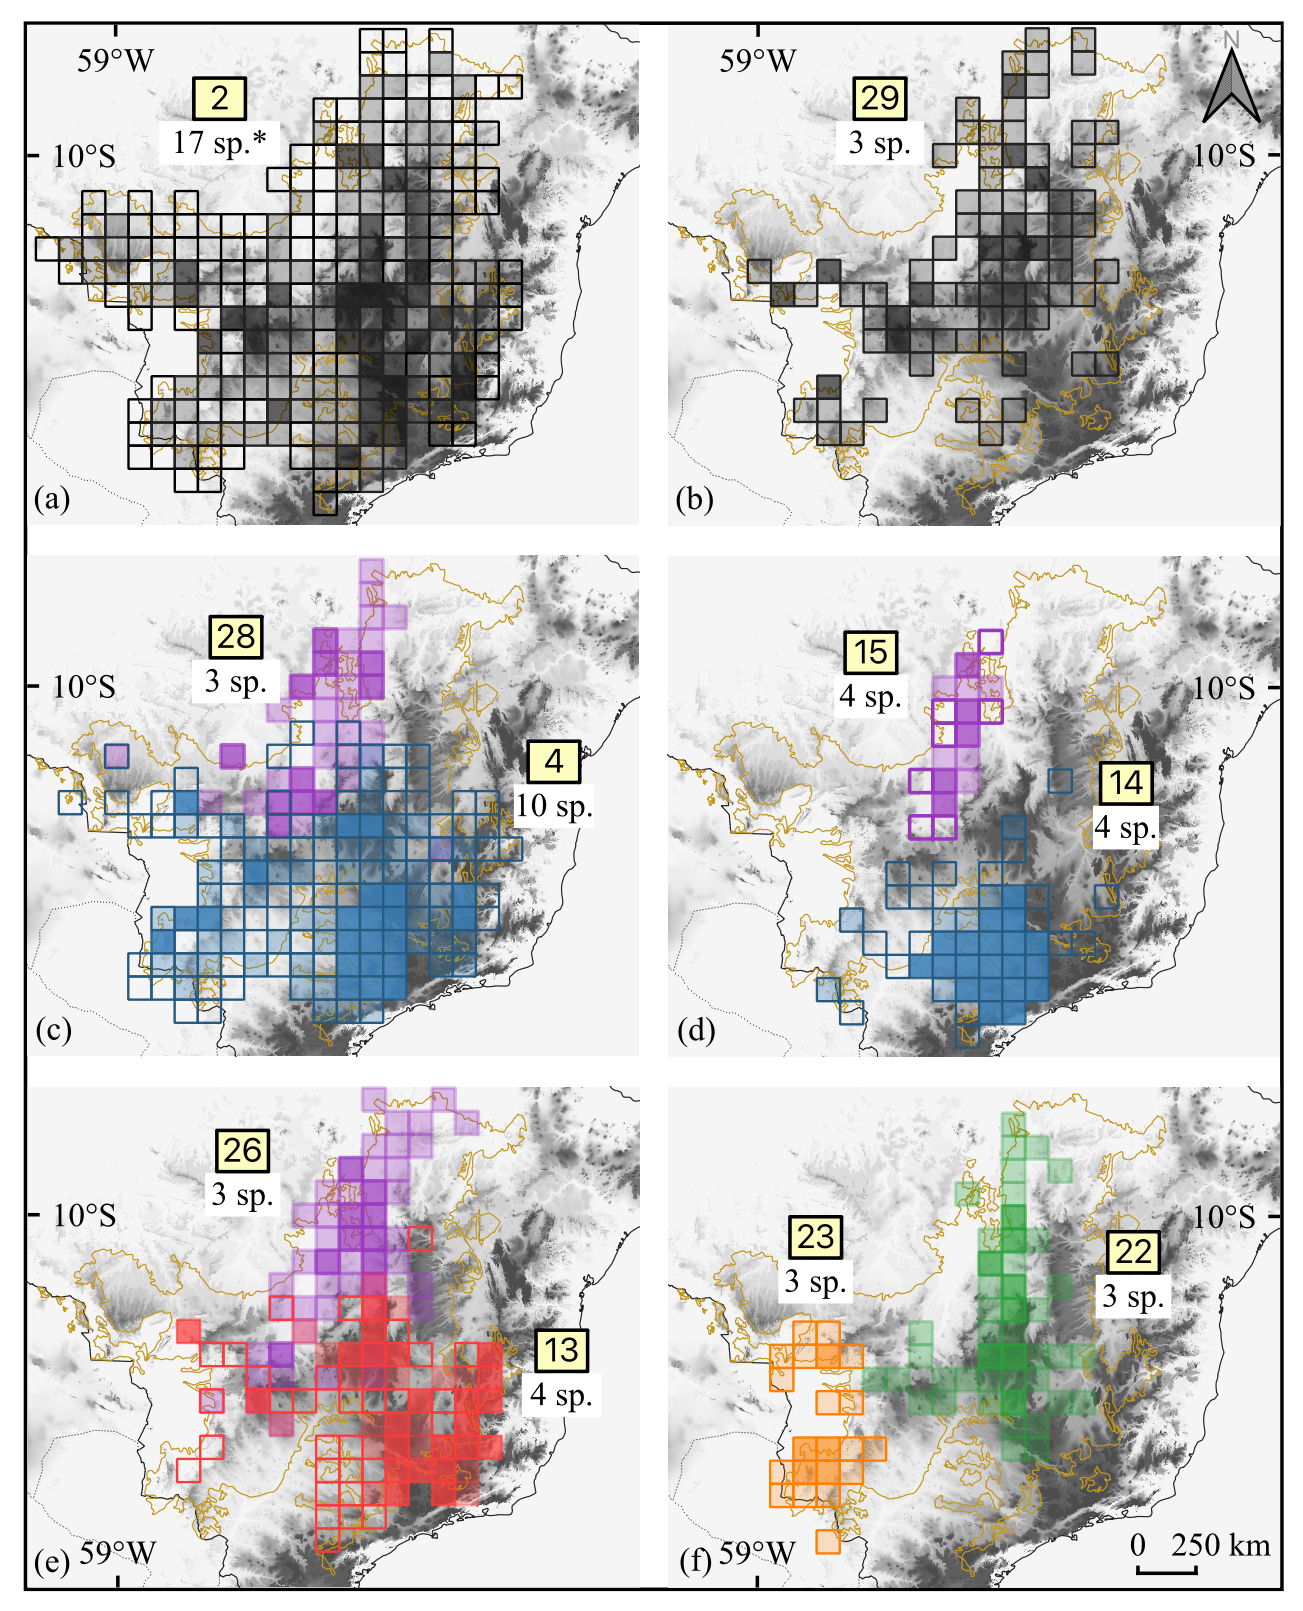
\includegraphics[width=150mm]{Fig c2-2}
	\caption[Widespread and partial Biotic Elements (BEs)]{\footnotesize Widespread and Partial Biotic Elements (BEs) composed of endemic terrestrial vertebrates in the Cerrado (limits represented by the yellow line). Biogeographical units named according to the overall region occupied by intermediate cells (>30\% of the component species), core cells (>70\% of the component species) and the major topographic units, when possible: (a) 2 - Whole Cerrado. (b) 29 - Northwestern Cerrado. (c) 4 - Southern Cerrado/Upper Paraná (La Plata) basin; 28 - Roncador Range/Araguaia basin. (d) 14 - Paulistânia/Upper Paraná (La Plata) basin; 15 - Middle Araguaia River valley. (e) 13 - Southeastern Cerrado; 26 - Araguaia basin. (f) 22 - Tocantins basin; 23 - Pantanal/Upper Paraguay basin. Asterisks indicate BEs composed of all groups of terrestrial vertebrates. Elevation is divided into four shades of grey, with the two lighter shades representing 0-250 and 250-500 m respectively, and the darker representing 500-750, 750-1,000, and above 1000 m.The contrast between the lighter and darker shades highlight the threshold separating “Plateau” from “Depression” units (\citealp[see][]{Silva1997}). The numbers in the yellow squares are the BE number. The number of species (sp.) in each unit is below the BE number.}
	\label{fig:fig2-2}
\end{figure}

\subsection{\textit{Elevation and BEs}}\label{sub:top}

The elevational range of all unique species records varied from zero to 2,067 m, with a median of 611 m. Species from plateaus or depressions tended to compose the same elements ($\chi^2$  = 198.45, \textit{df} = NA, \textit{p} <  0.001, for all species forming BEs, and $\chi^2$ = 121.04, \textit{df} = NA, \textit{p} <  0.001 for species forming restricted BEs only), corroborating the hypothesis that altitudinal isolation may be an important driver of Cerrado endemism and regionalization patterns (\autoref{fig:fig2-3}). Based on the distribution of elevation records, we found 14 Plateau BEs, 12 Depression BEs and three general BEs (see \autoref{tab:tab2-1} and \autoref{fig:fig2-3}).

\begin{figure}[htb]
	\centering
	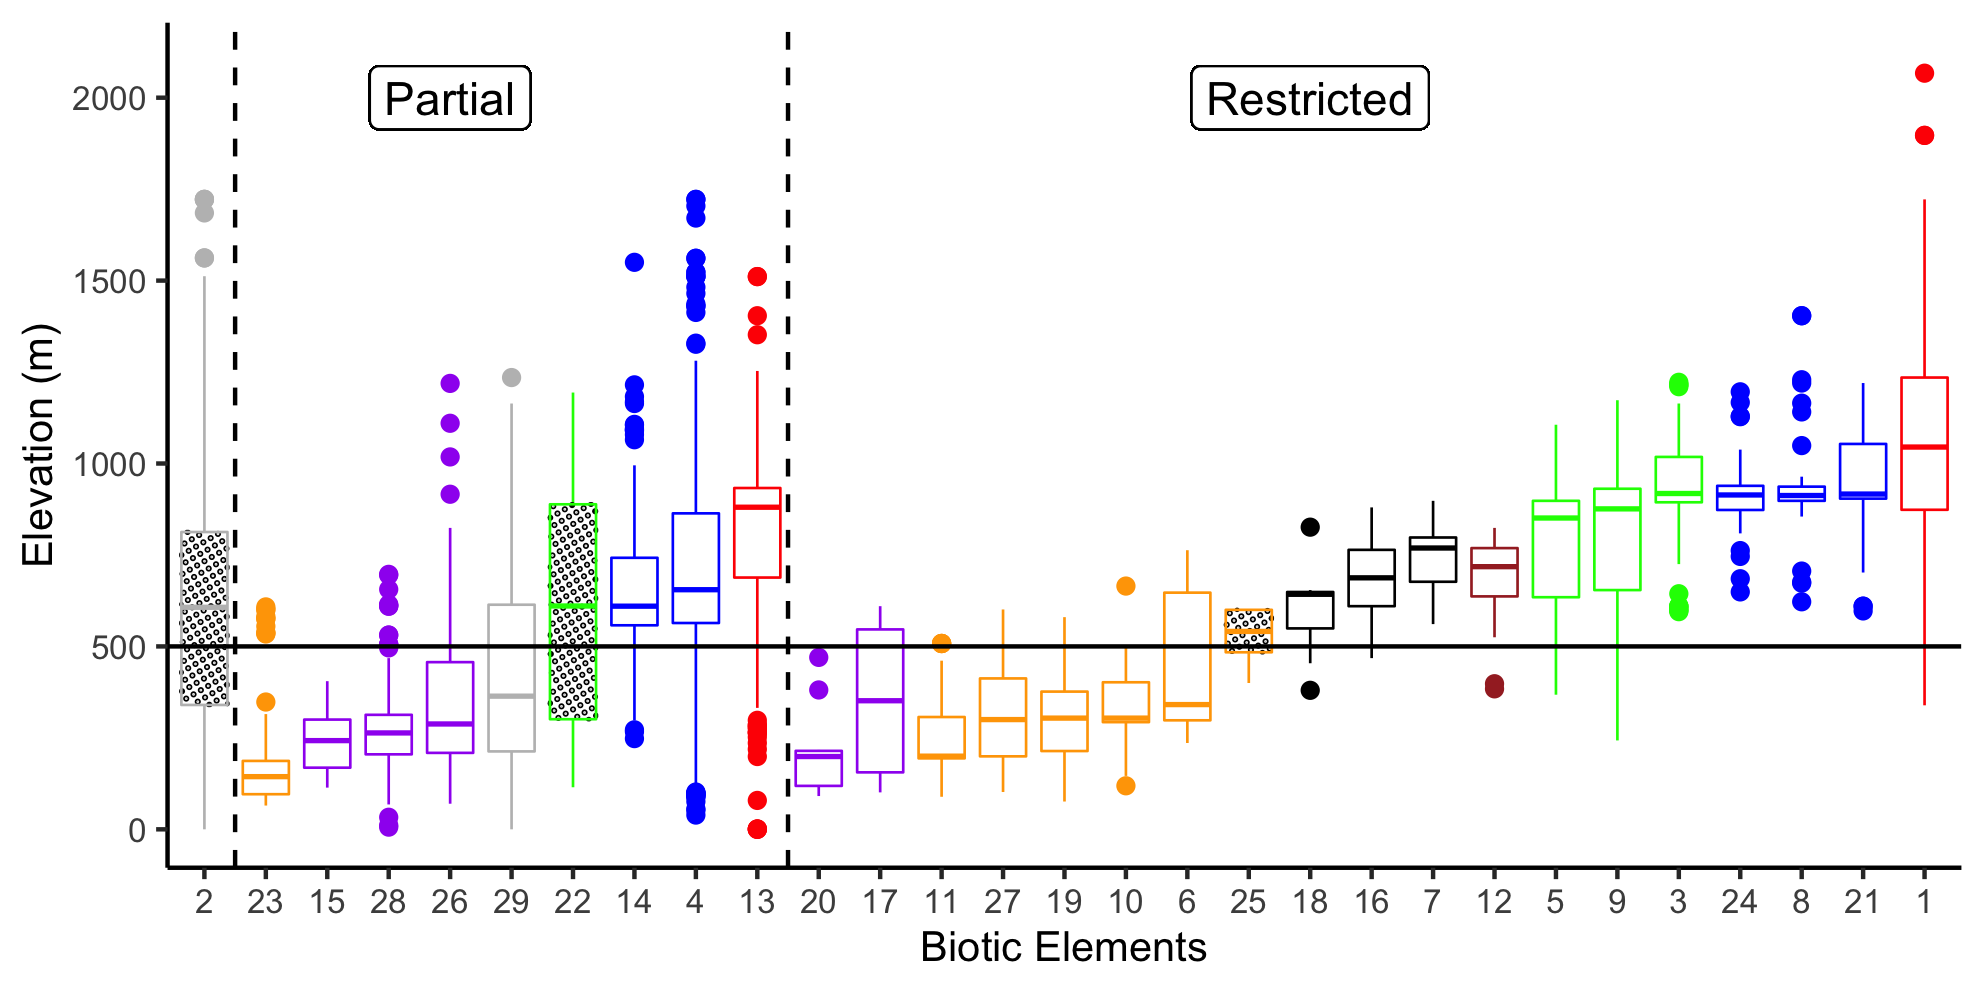
\includegraphics[width=160mm]{Fig c2-3}
	\caption[Biotic Elements (BEs) elevational range]{\footnotesize Elevation range of Biotic Elements formed by endemic terrestrial vertebrates in the Cerrado. Boxes represents the interquartile range (IQR: Q1 - 25 percentile and Q3 - 75 percentile), composing 50\% of all elevational records. The line of central tendency is the median. Whiskers represent “Maximum” (Q3 + 1.5*IQR), and “Minimum” (Q1 - 1.5*IQR). The points above or below the whiskers are outliers. Units are coloured as in \autoref{fig:fig2-1} and \autoref{fig:fig2-2} and according to general geographical position in the Cerrado (e.g. Northern - Purple; Central western - Brown; Western - Orange; Central - Green; Eastern - Black; Southern - Blue; Southeastern - Red). The horizontal line represents the threshold separating “Plateau” from “Depression” units (\citealp[see][]{Silva1997}). “General” Biotic Elements are filled with circles (see \nameref{sup:2-s1}).}
	\label{fig:fig2-3}
\end{figure}

Biotic Elements with the lowest values of elevation are concentrated in the western portion of the Cerrado, near contacts with Amazonia and wetlands of the Paraguay or Guaporé/Itenez drainages. BEs presenting the highest altitudinal ranges are located in central and southeastern portions of the Cerrado, at the core of the Brazilian Shield. Among partial BEs, all but BE 22 could be assigned to an elevation category, despite the high elevational variability within those units (\autoref{fig:fig2-3}). Similarly, all restricted BEs except BEs 25, could be assigned to one of the elevational categories proposed above (\autoref{fig:fig2-3}).

We found no statistical differences in number of species per vertebrate group in BEs from different elevational categories ($\chi^2$ = 15, \textit{df} = 12, \textit{p} = 0.2414), indicating that all vertebrate groups are equally prone to form plateau or depression units. However, for restricted BEs (units with the smallest elevational variability), amphibians and birds were much more frequent in plateau units (89\% and 86\% of the species, respectively), while the remaining groups were almost evenly distributed in both categories, despite the general prevalence of species in plateau units (\autoref{tab:tab2-3}).

\begin{table}
	\centering
	\caption[Terrestrial vertebrate classes proportion in Biotic Elements (BEs) elevational categories]{\small Absolute number and approximate percentages of species composing restricted BEs in each elevational category. Percentages are relative to the total number of species of a given group assigned to BEs. In parenthesis the number of units per category.}
	\label{tab:tab2-3}
	\vspace{\bigskipamount}
	\footnotesize
	\begin{tabular}{c c c c c c c}
		\hline
		& Total & Amphibians & Reptiles & Birds & Mammals\\
		\hline
		Plateau & 93 - 76\% (10) & 56 - 89\% (10) & 23 - 59\% (8) & 6 - 86\% (2) & 8 - 62\% (4)\\
		Depression & 29 - 24\% (7) & 7 - 11\% (4) & 16 - 41\% (6) & 1 - 14\% (1) & 5 - 38\% (4)\\
		\hline
	\end{tabular}
\end{table}

\section{Discussion}

Our results, based on an extensive revised point locality database, revealed congruent endemism patterns for Cerrado terrestrial vertebrates, and detected non-random clusters of co-distributed species. The fact that all terrestrial vertebrate groups were proportionally prone to be assigned to BEs or to the noise component, independent of the number of species per group (see \autoref{tab:tab2-2}), indicates that no idiosyncratic trait (range size; dispersal ability) has influenced the presence of different terrestrial vertebrate groups in the recovered BEs. These multi-taxon range clusters represent significantly segregated biotas separated by altitudinal compartments (plateaus x depressions), corroborating previous hypotheses on the role of geomorphological changes as major determinants of Cerrado endemism \citep{Silva1997, BrownGiff2002, Nogueira2011}. Indeed, vicariant isolation in depressions and plateaus along the Brazilian shield as a result of Neogene orogeny has been pointed as the most plausible explanation for genetic divergence in the frog genus \textit{Dermatonotus}, widespread in central portions of South America \citep{Oliveira2018}.

However, corroborating major predictions of the vicariant model does not prove that the recovered pattern was indeed a result of vicariance \citep{Hausdorf2002}. Vicariant scenarios could be further tested using timed phylogenies and biogeographical barriers, under explicit historical biogeographical analyses \citep{Hausdorf2002, Hennig2004}. Biotic Elements are the primary spatial units, or necessary first step, to test if the recovered patterns were formed in response to the same general historical events/barriers or a result of secondary dispersal or similar processes \citep{Hausdorf2002}. Whether or not a direct result of vicariance, species forming BEs share the same areas, representing, at least, non-random, non-arbitrary geographical units, objectively derived from raw distribution data \citep{Hausdorf2002}.

The regionalization pattern recovered herein corroborates and complements results based on data for the Cerrado herpetofauna \citep{Nogueira2011, Azevedo2016} and supports the hypothesis that repeated and congruent patterns may be general and ruled by the same major scale determinants. Six out of seven units in \citet{Nogueira2011} and 13 out of 16 in \citet{Azevedo2016} were also recovered based on our terrestrial vertebrate dataset. Only three BEs (“Chapada das Mesas”, “Serra da Borda” and “Roncador plateau”) detected by \citet{Azevedo2016} were not recovered in the present study, and their component species  were assigned to the noise component in our analyses. Moreover, some species assigned to these previous units were not included in our analysis due to taxonomic changes or uncertainties \citep{Frost2020, Uetz2020}. On the other hand, units such as BE 19 (“Bodoquena”), BE 24 (“Campos Gerais, Paraná state”) and BE 27 (“Upper Guaporé Valley”) had never been detected before, indicating that Linnean and Wallacean shortfalls posed limitations for our understanding of biogeographical patterns and processes in the Cerrado. Some of the BEs detected here represent smaller portions of previously detected larger units. For example, the “Paraguay-Guaporé” unit of \citet{Nogueira2011} was split into the “Serra das Araras/Paraguay-Jauquara basin” (BE 10), “Huanchaca plateau/Guaporé River valley” (BE 11), and “Parecis plateau” (BE 25) units (see \nameref{sup:2-s1}). This refinement indicates that taxonomically diverse datasets increase the potential to unravel previously overlooked biogeographical patterns while also providing support and more detail for well-established biogeographical units.

Furthermore, most of the ten floristic provinces detected for Cerrado endemic species of the plant genus Mimosa \citep{Simon2000} are congruent with BEs detected for endemic terrestrial vertebrates, including the “Western Cerrado”, “Southern Cerrado”, “Serra do Espinhaço South”, “Serra do Espinhaço North”, “Central Western Cerrado” and “Central Highlands” provinces. Additionally, the cores of BEs 4, 15, and 23, as well as the restricted BE 5, are partially congruent, respectively, to the floristic districts “South”, “North-West”, “South-West”, and “Central” proposed by \citet{Francoso2020}. These large phytogeographical units, however, fail to detect and describe more detailed internal complex endemism patterns, and generally correspond to our partial BEs. Moreover, these linearly defined, perfectly allopatric districts (as most traditional biogeographical units, \citealp[see][]{Hausdorf2002}), fail to account for peripheral contact and partial sympatry that are characteristic of raw distribution data, and that may be typical of natural, data-driven biogeographical units \citep{Hausdorf2002}.

The high proportions of amphibians, reptiles and mammals in restricted BEs indicates that these groups might respond similarly to biogeographical drivers, as opposed to birds, that were proportionally richer in widespread or partial BEs (see \autoref{tab:tab2-2}). Birds have the largest geographical distributions among vertebrates \citep{Gaston1996}, and their high mobility \citep{Sick1997} may mask patterns originated by vicariance due to post-speciation dispersal \citep{Hausdorf2002}. The fact that birds were richer in widespread BEs, while relatively rare in partial or restricted BEs, may be a result of this greater dispersion capacity and relatively wide ranges. However, birds were still important components of most recovered BEs, especially in plateau units, indicating that dispersal has not fully erased significant regionalization patterns in this group. In fact, three of the four areas of avian endemism for the Cerrado proposed by \citet{Silva1997} were recovered as BEs: “Espinhaço Plateau” = Espinhaço mountain range” - BE 1, “Araguaia River Valley” = Araguaia River basin” - BE 15, and “Central Goiás Plateau” = “Upper Parnaíba region” - BE 21.

Depression units showed the lowest number of species in their composition, corroborating the idea that endemism predominates along isolated plateaus \citep{Nogueira2011}. However, the western portion of the Cerrado, where most depression units are concentrated, is markedly less explored (\citealp[see][]{Oliveira2016}), and therefore, may harbour important areas for further surveys and species taxonomic assessment. For instance, two out of seven restricted depression units are novel BEs, and four are fine-scale splits from larger, previously detected units. This suggests that systematic regional fieldwork is still necessary to test the units proposed here and to unravel finer scale biogeographical units.

Although most BEs showed a predominant elevation range type (plateaus/depressions), most were formed both by plateau and depression species. This indicates that topographical changes, possibly generated by major tectonic shifts along the Miocene and Pliocene (\citealp[see][and references therein]{Silva1997, TeixeiraJr2016,Oliveira2018}) may have acted simultaneously on the isolation of fragmented plateaus and disconnected depressions, interpreted as mutual “soft” barriers (\citealp[see][]{TeixeiraJr2016}). These major continental topographical changes are now reflected in the Cerrado complex endemic faunas, regionalized according to conspicuous Cerrado topographical units, including the central Brazilian Plateau, Chapada dos Guimarães plateau, Parecis plateau, Paraguay depression, Espinhaço range, Araguaia and Tocantins depression, among many others, which largely correspond to the major subdivisions of the Brazilian shield \citep{Silva1997}. The complex and nested pattern shown by these units (see \autoref{fig:fig2-1}) suggests that multiple and sequential topographical changes have successively fragmented and shaped ranges in the Cerrado (\citealp[see][]{Silva1997, Nogueira2011, Vasconcellos2019}).

Although previous phylogeographical analyses \citep{Santos2014, LimaRezende2019, Vasconcellos2019} did not recognize distinct species within the widespread taxa analysed, they point to a strong genetic structure coincident with some of our proposed units. \citet{Santos2014}, for instance, revealed three major genetic units for the Cerrado endemic lizard \textit{Micrablepharus atticolus} Rodrigues 1996 corresponding roughly  to our BEs 4, 29 and 26, respectively. Future phylogeographical studies may consider our results relevant to the interpretation of their findings, as we predict that ranges of cryptic species within widespread taxa may be congruent with our biogeographical units (\citealp[see][]{Vasconcellos2019}). Similarly, BEs would also aid in delimiting ranges of poorly studied or newly described species and by providing significant boundaries to range predictions in species distribution modelling \citep{Franklin2010, Raxworthy2003}.

As Biotic Elements analysis detects multiple regionalized biotas, providing support to allopatric speciation and vicariance (\citealp[][]{Hausdorf2003, Nogueira2011, Azevedo2016}; present study), we posit that new species descriptions in the Cerrado will tend to replicate the spatial patterns detected for terrestrial vertebrates (which, in turn, largely coincides with floristic endemism, \citealp[see][]{Simon2000}). Our broad regionalization patterns may serve as a template for the discovery of new species (and biogeographical patterns) in less studied groups such as fishes, invertebrates or vascular plants. We may be approaching a consensus on the regionalization of the richest and most threatened savanna of the planet. Further analyses incorporating a more inclusive and representative taxonomic dataset should provide robust tests for this hypothesis. The inclusion of recent data on species ranges and endemism resulted in the discovery of novel biogeographical patterns already under threat in the light of the rapidly changing land use scenario in central Brazil \citep{Strassburg2017, Liuetal2022}.

Topographical differences between plateaus and depressions were interpreted as major drivers of past climatic stability in central Brazil, with plateaus pointed as climatic refugia in Pleistocene climate shifts, conserving stable savanna/gallery forest mosaics over time \citep{BrownGiff2002, Vasconcellos2019}. Moreover, plateaus in the Serra Geral (BE 7) and Espinhaço Range (BE 1) were pointed as potential Cerrado refugia in past climatic fluctuations \citep{Werneck2012}. In fact, many restricted BEs were associated with eastern highland plateaus, which might support the idea that climatic stability (even though only indirectly, \citealp[see][]{Marin2018}) and topography were important for the origin of Cerrado endemic species \citep{Silva1997, LimaRezende2019, Vasconcellos2019}. Moreover, if past climate refugia were concentrated on plateaus \citep{Werneck2012}, most of our restricted BEs may represent critical areas for conserving biotas under climate change scenarios. These areas were important for the history of Cerrado endemic biotas and may also be critical for their conservation in an uncertain future.

Our results indicate that the origin, history and fate of biogeographical units in the Cerrado seem highly connected to historical landscape changes and topographical complexity, in agreement with previous studies \citep{Silva2002, Nogueira2011}. We also highlight the importance of revised point-locality databases, incorporating planned inventories and accumulated revised voucher specimens as a critical first step for biogeographical analyses and biodiversity syntheses (\citealp[see][]{Hausdorf2002, Nogueira2019}). Our general, detailed and complex bioregional patterns, including narrow ranged, recently described and highly irreplaceable biotas, can be decisive to inspire broader discussions on the origin and destiny of endemism in the richest and most threatened savanna on the planet.

\pagebreak

\section{Supporting information}\label{sec:supinfo-2}
\subsection*{Appendix S1}\label{sup:2-s1}
 
 List of endemic terrestrial vertebrates composing each Biotic Element (BE) or Noise component in the Cerrado, and a description of ranges and BEs according to range extent and topographical position in the Cerrado. BEs previously detected as composed of a given species in \citet{Nogueira2011} and \citet{Azevedo2016} are also provided. Appendix S1 is provided in .xlsx format.

\subsection*{Appendix S2}\label{sup:2-s2}

\begin{table}[H]
	\caption*{\small Combinations of the parameters \textit{cutdist} and \textit{nnout} compared for the detection of Biotic Elements through hierarchical clustering in package ‘prabclus’. The value of \textit{k} with our dataset is 8.5. \textbf{Bold} values are the combination choosen to map Biotic Elements. Green backgrounds are all combinations with previzualized and compared results.}
	\label{}
	\centering
	\vspace{\bigskipamount}
	\footnotesize
	\begin{tabular}{c l r r r r r r r r r}
		\hline
					&\textbf{Cutdist}	& \textbf{0.1}	& \textbf{0.15}	& \textbf{0.2}	& \textbf{0.25}	& \textbf{0.3}	& \textbf{0.35}	& \textbf{0.4}	& \textbf{0.45}	& \textbf{0.5}\\
		\hline	
					&Noise	& 175	& 112	& 56	& 28	& 10	& 5	& 4	& 1	& 1\\
nnout = 1	&BEs	& 50	& 52	& 52	& 43	& 31	& 27	& 21	& 13	& 11\\
					&Prop	& 3.5	& 2.15	& 1.08	& 0.65	& 0.32	& 0.19	& 0.19	& 0.08	& 0.09\\
		\hline
					&Noise	& \cellcolor{lightgray}233	& \cellcolor{lightgray}\textbf{158}	& 96	& 52	& 18	& 15	& 12	& 3	& 1\\
nnout = 2	&BEs	& \cellcolor{lightgray}21	& \cellcolor{lightgray}\textbf{29}	& 32	& 31	& 27	& 22	& 17	& 12	& 11\\
					&Prop	& \cellcolor{lightgray}11.1	& \cellcolor{lightgray}\textbf{5.45}	& 3	& 1.68	& 0.67	& 0.68	& 0.71	& 0.25	& 0.09\\
		\hline
					&Noise	& 260	& \cellcolor{lightgray}197	& \cellcolor{lightgray}114	& 73	& 30	& 24	& 15	& 6	& 4\\
nnout = 3	&BEs	& 12	& \cellcolor{lightgray}16	& \cellcolor{lightgray}26	& 24	& 23	& 19	& 16	& 11	& 10\\
					&Prop	& 21.67	& \cellcolor{lightgray}12.31	& \cellcolor{lightgray}4.38	& 3.04	& 1.3	& 1.26	& 0.94	& 0.55	& 0.4\\
		\hline
					&Noise	& 280	& 217	& \cellcolor{lightgray}142	& 85	& 42	& 32	& 23	& 6	& 4\\
nnout = 4	&BEs	& 7	& 11	& \cellcolor{lightgray}19	& 21	& 20	& 17	& 14	& 11	& 10\\
					&Prop	& 40	& 19.73	& \cellcolor{lightgray}7.47	& 4.05	& 2.1	& 1.88	& 1.64	& 0.55	& 0.4\\
		\hline
					&Noise	& 290	& 227	& 162	& 95	& 47	& 37	& 28	& 6	& 4\\
nnout = 5	&BEs	& 5	& 9	& 15	& 19	& 19	& 16	& 13	& 11	& 10\\
					&Prop	& 58	& 25.22	& 10.8	& 5	& 2.47	& 2.31	& 2.15	& 0.55	& 0.4\\
		\hline
	\end{tabular}
\end{table}

\subsection*{Appendix S3}\label{sup:2-s3}

Grid system (1ºx1º) used in the Biotic Element analysis, based on the Cerrado ecoregion limits proposed by \citet{Dinerstein2017} with the same grid origin as used in \citet{Azevedo2016}. Appendix S3 is provided in .zip format including .shp and supporting files.

\subsection*{Appendix S4}\label{sup:2-s4}

Presence-absence matrix based on the intersection of verified point-locality records and the grid system provided as Appendix S3 in Supporting Information. Lines are species; columns are grid cells, column names are grid cells “ID”. Appendix S4 is provided in .csv format.

%%%%%%%%%
% CAPÍTULO 3 %
%%%%%%%%%

\chapter[Priority Areas of Cerrado hotspot]{\centering{How habitat loss and fragmentation are reducing conservation opportunities for vertebrates in the most threatened savanna of the World}}\label{chap3}

\begin{resumo}[\normalsize Abstract]
	\noindent
	Effective, resilient and strategic protected area networks are essential to protect biodiversity and human welfare, especially in vulnerable biodiversity hotspots. This is the case in the Brazilian Cerrado, the richest tropical savanna, and a deforestation front worldwide. Worryingly, the rate of habitat conversion in Cerrado greatly reduces opportunities to conserve its biodiversity. Herein, using the most comprehensive database on the distribution of Cerrado endemic terrestrial vertebrates, we mapped conservation priority areas and evaluated how and to what extent habitat loss and fragmentation reduce conservation opportunities. Priority areas are scattered throughout the Cerrado. Larger priority areas are concentrated in the northern portion of the region. Southern priority areas are small, scattered, and isolated. During the last 35 years, opportunities to conserve large contiguous areas have significantly decreased, hampering the representation of key endemic species. However, as most endemic vertebrates are small ranged, modest but well located increments in total protected area will result in significant overall improvements in the PA system. Protecting the largest priority areas identified here is urgent and mandatory, while using habitat restoration as a key activity to promote connectivity among smaller priority areas, especially in the southern portion of this hotspot.
	
	\vspace{\medskipamount}
	\noindent
	\textbf{Keywords}: Cerrado biodiversity hotspot; Conservation planning; Deforestation hotspots; Endemism; Habitat fragmentation; Terrestrial vertebrates

\end{resumo}

\setlength{\parindent}{1cm}

\section{Introduction}\blfootnote{Esse capítulo é a versão na íntegra do artigo já publicado na revista \textit{Perspectives in Ecology e Conservation} e pode ser acessado em: \url{https://doi.org/10.1016/j.pecon.2023.02.004}. Esse texto foi produzido com a colaboração de: Bruna Espinoza Bolochio, Ana Paula Carmignotto, Ricardo Jannini Sawaya, Luis Fabio Silveira, Paula Hanna Valdujo, Cristiano de Campos Nogueira e Javier Nori}

Creating and managing strategic protected areas (PAs) is fundamental for biodiversity conservation. They are essential to reaching nature-based solutions for adaptation to global changes \citep{Maxwell2020}, maintaining wildlife populations \citep{Geldmann2013}, and ensuring long-term maintenance of nature’s contributions to people \citep{Diaz2018}. Worryingly, despite the sustained increase in numbers of PAs globally \citep{Maxwell2020}, historically PA allocation has not met scientific criteria, being influenced by economic activities and opportunism \citep{Margules2000}. This is particularly true in economically productive ecoregions \citep{PrietoTorres2022} such as the Cerrado hotspot \citep{Strassburg2017, Vieira2019}. In this context, science has developed systematic conservation planning protocols to achieve resilient and effective PAs, based on objective criteria and relevant information \citep{Margules2000, DiMinin2014}.

Habitat loss and fragmentation are the main causes of species extinctions and declines, hampering population viability of most threatened species \citep{IPBES2019, Grande2020}. Conservation opportunities for efficient PAs exponentially decrease as habitat fragmentation advances \citep{Nori2013}. The protection of contiguous patches of natural ecosystems is necessary for the conservation of most key and threatened species, ecological processes, and nature’s contributions to people \citep{Diaz2018}. Sadly, current rates of conversion of the few remaining natural habitats in deforestation hotspots, such as the Brazilian Cerrado, make this unlikely.

The Brazilian Cerrado is the richest savanna in the world, with high levels of endemism \citep{Strassburg2017}. However, this biodiversity hotspot has recently suffered rampant natural habitat loss due to a combination of low legal protection and increased demand for commodities \citep{Pacheco2021}. Additionally, the Cerrado is one of the eight deforestation frontiers undergoing high rates of recent deforestation, with conversion now concentrated in the northern portion of the region, where natural habitats persist as large contiguous areas \citep{Strassburg2017}. Given the context, efficient policy-making toward their conservation is imperative.

Herein, using the most comprehensive revised point-locality database on endemic terrestrial vertebrates of the ecoregion to date, we aimed (i) to determine priority areas for the conservation of Cerrado endemic terrestrial vertebrates; (ii) to determine the increase of habitat fragmentation of priority areas as the agricultural frontier advances; and (iii) to estimate the loss of conservation opportunities over time under current deforestation rates.

\section{Materials and Methods}
\subsection*{\textit{Disclaimer}}

No artigo original \citep{VieiraAlencar2023}, o texto publicado contém uma versão reduzida dos materiais e métodos desse trabalho e adicionamos um apêndice ao material suplementar do artigo, nomeado \textit{Extended methods}. No entanto, aqui na tese optei por apresetar diretamente a versão completa dos materiais e métodos.

\subsection{\textit{Study area}}

The Cerrado is the second largest South American phytogeographical domain, surpassed in extension only by Amazonia and occupying a central position in the Neotropical region, being dominated by upland savannas and grasslands \citep{Absaber1998}. It is bordered in the northwest by the Amazon and in the east by the Atlantic Forest, and forms the South American diagonal of open vegetation together with the Caatinga in the northeast and the Gran Chaco in the southwest. This savanna ecoregion is dominated by heterogeneous xeromorphic vegetation ranging from areas dominated by grasslands, with small shrubs (campo limpo), to areas formed by almost closed canopy woodland (cerradão; \citealp{Eiten1972, Ratter1997}). However, the Cerrado has been intensively modified by the conversion of its natural vegetation into croplands and planted pastures, which implies deforestation rates higher than the Amazon, coupled with less legal protection of its outstanding endemic biodiversity \citep{Strassburg2017}.

We adopted the limits of the Cerrado ecoregion as proposed by \citet{Dinerstein2017}, which is an ecoregion approach initially based on the Cerrado limits of the Instituto Brasileiro de Geografia e Estatística (\citealp{IBGE1993}; \citealp[see][]{Olson2001}). As we included a variable containing land use information, available mainly for the Brazilian territory (\citealp{MapBiomas2022}; see below), we retained the Brazilian portion of the ecoregion corresponding to 99.23\% of the Cerrado, after removing its small portions in Paraguay and Bolivia.

\subsection{\textit{Species and occurrence records}}

Our database is composed of 13,790 unique records of 337 Cerrado endemic terrestrial vertebrates, including 124 amphibian anurans, 66 lizards, 63 snakes, 45 birds and 39 mammals, with a mean of 2,758 distribution records per group (\textit{sd} = 2,097), and a mean of 41 records per species (\textit{sd} = 93). This is the most comprehensive database of geographic information on Cerrado endemic terrestrial vertebrates to date. These records are based on planned field surveys to cover previous sampling gaps and revision of vouchered specimens deposited in scientific collections (\citealp[see details in][]{Nogueira2009, Valdujo2012, Nogueira2019, Carmignotto2022}), complemented by revised literature data. We considered endemic species, those with ranges fully or largely coincident with the approximate limits of the Cerrado provided in \citet{Dinerstein2017}. Species with marginal records in transitional areas between the Cerrado and other domains, but with local ranges associated with typical environments of the Cerrado were also considered endemic, due to their possible historical association to once continuous areas of Cerrado. The nomenclature follows specific literature for each vertebrate group (\citealp{Frost2020} for anurans, \citealp{Uetz2020} for lizards/amphisbaenians, \citealp{Nogueira2019} for snakes, \citealp{Pacheco2021birds} for birds, and \citealp{Abreu2021} for mammals).

We departed from verified point-locality records and created normalized heatmaps to represent species distributions. Heatmaps represent a simple extrapolation of a species point occurrence, highlighting regions with a high density of records and giving less weight to pixels towards the edge of the buffered heat core. The highest values are attributed to the exact location where the species was recorded and lower values are continuously attributed to pixels further away from the verified occurrence \citep{QGISUserGuide}. This approach allows us to give relatively less importance to pixels distant from the original species record without disregarding the potential of surrounding areas to contain suitable environmental conditions for a given species. Also, compared with other commonly used methods based on correlative extrapolations, and considering the completeness of our database, heatmaps are only based on the distributional records, minimizing potential commission errors as a consequence of spurious projections. Finally, using heatmaps avoids overlooking potentially important areas around a species record (e.g. decreasing the effect of omission errors) while also dealing with putative commission errors by decreasing the importance of a pixel according to its distance from the verified occurrence. 

We created the heatmaps using the Kernel Density Estimation tool, available in QGIS 3.24 \citep{QGIS}. In order to create a spatially representative extrapolation we defined the radius of 0.5º providing a 1º circular area around the species record. In the Cerrado, 1ºx1º grid systems have been used in studies on vertebrates diversity and historical biogeographical patterns (\citealp[e.g.][]{DinizFilho2008, Azevedo2016}), and prioritization analyses for conservation purposes \citep{DinizFilho2008b}. We used the resolution of $\sim$20km\textsuperscript{2} (0.041667º) and grid origin based on the WorldClim 2.5 arc minutes bioclimatic database \citep{FickHijmans2017}, to allow further comparative analyses that might consider those climatic variables (\citealp[see for example][]{Lemes2020}) and to guarantee a spatial resolution that would optimize computational requirements without excessively downgrading land use variables. We normalized the estimated heat values by dividing the resulting raster file by the maximum value of the raster, therefore obtaining a continuous output from zero to one for all species.

\subsection{\textit{Estimation of Priority Areas}}

We used Zonation 4.0 \citep{Moilanen2014} to identify priority areas for the conservation of Cerrado endemic terrestrial vertebrates. The software implements hierarchical prioritization of areas based on the distribution of biodiversity features (e.g. species, ecosystem services) considering predefined user input weights for each feature. In this case, each pixel contains information on the occurrence of a given biodiversity feature, and the algorithm continuously removes pixels with smaller values of the features of interest, progressively recalculating the importance of the remaining pixels and repeating this procedure until the last pixel in the study area is removed. Then, the pixels are hierarchically classified and the output of highly important areas can be displayed according to user-defined conservation thresholds.

Zonation allows for different “cell-removal rules”. Prioritizations were run under the \textit{Core Area Zonation} (CAZ) rule. In short, the CAZ rule identifies high-priority areas as those that present a high occurrence level of a single rare or highly weighted feature (for a more detailed explanation on different prioritization rules see \citealp{DiMinin2014}). This removal rule was selected given that selected input species are endemic to the Cerrado, and many are restricted to small portions of the study region. In this sense, Zonation is more likely to create an output that represents all species highlighting portions of the Cerrado that must be preserved to protect highly irreplaceable biodiversity features. To select areas optimal for expanding the PA network, we included existing PAs as a hierarchical mask \citep{DiMinin2014}. This approach leads to minimum costs to achieve conservation targets as it selects the best part of the landscape surrounding existing PAs, which are preferably retained as the first option in the analysis. The shapefile of PAs was downloaded from the World Database on Protected Areas \citep{IUCN2020} and cropped to the limits of the Cerrado. We included all PA categories, with strict and non-strict conservation goals, such as National and State Parks, Ecological Stations, and Private areas such as “APAs” and “RPPNs”, in our analysis. Only PAs with detailed geographic information were considered, excluding those represented only as a point locality. 

Zonation accounts for feature-specific weights prioritizing the protection of highly weighted biodiversity features (in this case species), which allows us to adapt the prioritization to our specific aims. To emphasize the importance of microendemic, threatened (VU, EN, CR) or poorly known (DD) taxa as a precautionary measure (\citealp[see][]{Nori2018}), we generated a simple index including both categories: distributional pattern and extinction risk. Our weighted index is the result of a multiplication of values from 1 to 3 (“widespread” = 1, “partial” = 2, and “restricted” = 3, \citealp[see][]{Nogueira2019}) for range size, and values from 1 to 5 according to the IUCN categories  (LC = 1, NT = 2, VU and DD = 3, EN = 4 and CR = 5; \citealp{IUCN2022}). Additionally, DD species described since 2010 and species currently not assessed by IUCN received the value of “2” in the extinction risk part of the index. This value represents a lower weight than weights assigned to species that remained classified as DD even after a decade of their description, while also represents a higher weight than that of taxa indisputably regarded as “Least Concern” for conservation purposes. The endemic rodent \textit{Juscelinomys candango} was not included in the analysis because according to IUCN it is classified as extinct.

In order to penalize pixels covered by anthropic land-uses, we included reclassified binary land-use maps (obtained from \citealp{MapBiomas2022}) as a negative variable with a strong weight (equal to the sum of all positive variables weights). These rasters preclude or minimize the possibility to assign a high conservation value to pixels covered by crops or urban areas (see details of the raster reclassification in the \nameref{sec:supinfo-3} - \nameref{sup:3-s1}). To assess how priority areas (and conservation opportunities) have changed as a result of land use and land cover (LULC) changes throughout the last decades, we repeated the analyses using land-use map scenarios from 1985 to 2020 \citep{MapBiomas2022} in intervals of five years and also considered a pristine Cerrado scenario (e.g. without any LULC changes). To simulate a “pristine Cerrado scenario” we classified the whole Cerrado area as “Natural”, so no pixel was down-weighted due to the presence of anthropic uses.

According to the Aichi Biodiversity Targets \citep{CBD2010}, protected area networks should represent at least 17\% of the world’s landmass (see Target 11; \citealp{CBD2010}). We also mapped a recently proposed threshold of 30\%, for the post-2020 global biodiversity framework \citep{Woodley2019}. Finally, to analyze the effect of LULC changes and resulting fragmentation on priority areas across time, we grouped patches of priority areas (i.e. connected pixels of the top 17\% of priority areas in each scenario) depending on their area. We used the following categories: “Large” for priority nucleus with area coverage equal to or larger than 1,000 km\textsuperscript{2}; “Medium” for priority nucleus with area coverage equal to or larger than 250 km\textsuperscript{2} and smaller than 1,000 km\textsuperscript{2}; and “Small” for priority nucleus with area coverage smaller than 250 km\textsuperscript{2}. We consider that continuous areas of more than 1,000 km\textsuperscript{2} represent enough available habitat for maintaining a viable population of most of the included species.

%%%%%%%%%%%
%SHORT VERSION%
%%%%%%%%%%%

%The Cerrado is the second largest South American phytogeographical domain, dominated by upland savannas and grasslands \citep{Absaber1998}. Herein, we adopted the limits of the Cerrado ecoregion as proposed by \citet{Dinerstein2017}.

%We compiled the most comprehensive revised point-locality database on Cerrado endemic terrestrial vertebrates to date, comprising 13,790 unique records of 337 species, including 124 amphibian anurans, 66 lizards, 63 snakes, 45 birds, and 39 mammals. These records are based on planned field surveys and revision of vouchered specimens in scientific collections, complemented by revised literature data.

%From verified point-locality records we created normalized heatmaps representing species distributions. Heatmaps are a simple extrapolation of species records, highlighting regions with a high density of records and giving less weight to pixels towards the edge of the buffered heat core. Compared to other commonly used methods based on correlative extrapolations, and considering the completeness of our database, heatmaps based only on point records minimize potential commission errors as a consequence of spurious projections. Finally, heatmaps avoid overlooking potentially important areas around species records (e.g. decreasing the effect of omission errors). We created heatmaps using the Kernel Density Estimation tool, in QGIS 3.24 \citep{QGIS}, with a radius of 0.5º around points, and a resolution of $\sim$20km\textsuperscript{2} (0.041667º). We normalized the estimated heat values by dividing the resulting raster file by its maximum value, therefore obtaining a continuous output from zero to one for all species.

%We used Zonation 4.0 \citep{Moilanen2014} to locate priority areas for the 337 studied species. The software implements hierarchical prioritization of areas based on the distribution of biodiversity features, considering predefined user input weights for each feature. We ran prioritizations under the Core Area Zonation (CAZ) rule. CAZ rule identifies high-priority areas as those presenting a high occurrence level of a single rare or highly weighted feature \citep{DiMinin2014}. This removal rule was selected given that the input species are endemic to the Cerrado, and many are restricted to small portions of the region. To select optimal areas for expanding the PA network, we included existing PAs as a hierarchical mask \citep{DiMinin2014}. We included all PA categories, with strict and non-strict conservation goals, such as National and State Parks, Ecological Stations, and private areas such as “APAs” and “RPPNs”, in our analysis.

%To emphasize the importance of small-ranged, threatened (VU, EN, CR) or poorly known taxa (DD), we generated a simple index including both categories. Our weighted index is the result of a multiplication of values from 1 to 3 (“widespread” = 1, “partial” = 2, and “restricted” = 3, \citealp[see][]{Nogueira2019}) for range size, and values from 1 to 5 according to IUCN extinction risk categories (LC = 1, NT = 2, VU and DD = 3, EN = 4 and CR = 5; \citealp{IUCN2022}). To avoid overestimating the importance of species not assessed by IUCN, and those classified as DD within less than ten years after description, these were weighted with the value “2” in the extinction risk ‘part’ of the index. This results in a higher weight than that of species in “Least Concern”  while not surpassing the weight of those still classified as DD ten years after description (e.g. higher weight = “3”, see above; \citealp{Morais2013}).

%To penalize pixels covered by anthropic land uses, we included reclassified binary land-use maps (obtained from \citealp{MapBiomas2022}; reclassification details in \nameref{sec:supinfo-3} - \nameref{sup:3-s1}) as a negative variable weighted as the sum of all positive variable weights. To assess how priority areas shifted according to land use and land cover (LULC) changes in the last decades, we repeated the analyses using land-use scenarios from 1985 to 2020 \citep{MapBiomas2022} in five years intervals, considering also a pristine Cerrado scenario (e.g. without LULC changes).

%According to the Aichi Biodiversity Targets \citep{CBD2010}, PA networks should represent at least 17\% of the world’s landmass (see Target 11; \citealp{CBD2010}). In addition to the 17\% target, we also mapped a recently proposed target of 30\% (post-2020 global biodiversity framework, \citep{Woodley2019}). Finally, to analyze the effect of LULC changes and resulting fragmentation on priority areas over time, we grouped priority areas (i.e. connected pixels) depending on their area (for additional details see the extended methods, Appendix S2).

\section{Results}

Of the 337 analyzed species, 262 (77.4\%) have been assessed by IUCN. Of those, 39 (11.5\%) are considered threatened, including 17 Vulnerable, 15 Endangered, and seven Critically Endangered (\nameref{sup:3-s2}). Sixty-one species are considered Data Deficient, of which 57 (93.4\%) were described more than 10 years ago. Amongst the 75 species not assessed by IUCN, 77\% (N = 58) are restricted-range species, and the remaining 23\% (N = 17) are partially-distributed species.

\begin{figure}[htb]
	\centering
	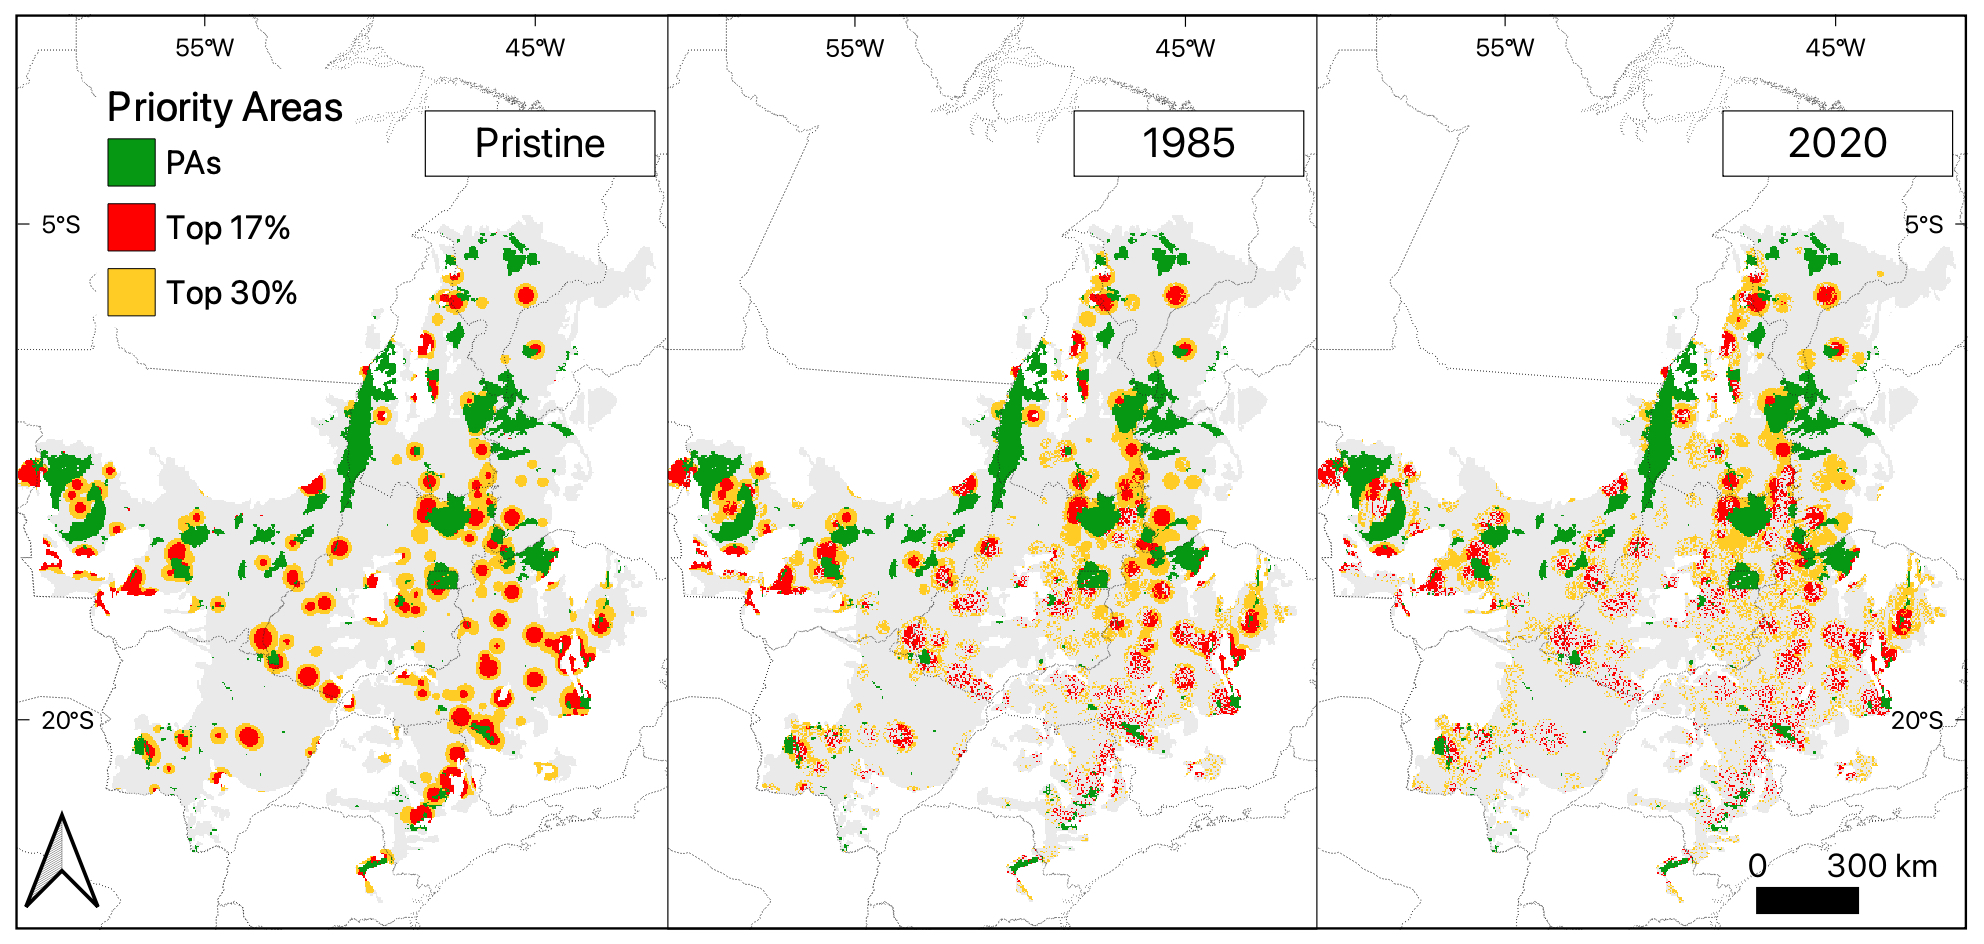
\includegraphics[width=160mm]{Fig c3-1}
	\caption[Priority areas for the conservation of Cerrado’s endemic terrestrial vertebrates]{\small Priority areas for the conservation of Cerrado endemic terrestrial vertebrate species, in three distinct land-use scenarios (Pristine, 1985 and 2020) and two conservation targets (top 17\% and 30\% of the ecoregion).}
	\label{fig:fig3-1}
\end{figure}

The current PA network covers 10.25\% of the Cerrado and putatively protects on average 21.47\% of the distributions of endemic terrestrial vertebrates. Four species are completely absent from the system (\nameref{sup:3-s3}). According to the prioritization, using the most recent land-use map (2020 scenario), protecting an additional 6.75\% of the region ($\sim$135,000 km\textsuperscript{2}, i.e. 17\% of the Cerrado) would represent at least 10\% of each distribution and increase the average representation to 43.5\%. In comparison, the protection of 30\% of top priority areas would increase this figure by an additional 12.7\%, representing at least 16.6\% of each distribution and an average of 56.2\% of mapped ranges. Detailed information on species representation in the current PA network and in each conservation target can be found in the supplementary material (\nameref{sup:3-s3}).

Despite the similar overall location of the top 17\% and 30\% priority areas, in the pristine scenario the priority areas were represented only by patches of continuous land, while in the 1985 and 2020 scenarios top priority areas also comprise some sparsely distributed discontinuous areas (\autoref{fig:fig3-1}). While in the pristine scenario continuous priority areas were spread across the Cerrado, in the 1985 and 2020 scenarios they were concentrated in the northern portion of the region, while largely segregated priority areas were mostly spread over the southern portion (\autoref{fig:fig3-1}). As for the patch size analysis of the top 17\% priority areas, opportunities to create, expand and connect PAs in large continuous extensions of natural habitats were concentrated in Mato Grosso, Minas Gerais, Goiás and Tocantins states (\autoref{fig:fig3-2}; \textbf{Box 1}). On the other hand, patches of medium to small priority areas are scattered throughout the southern portion of the region (\autoref{fig:fig3-2}).

\begin{figure}[H]
	\centering
	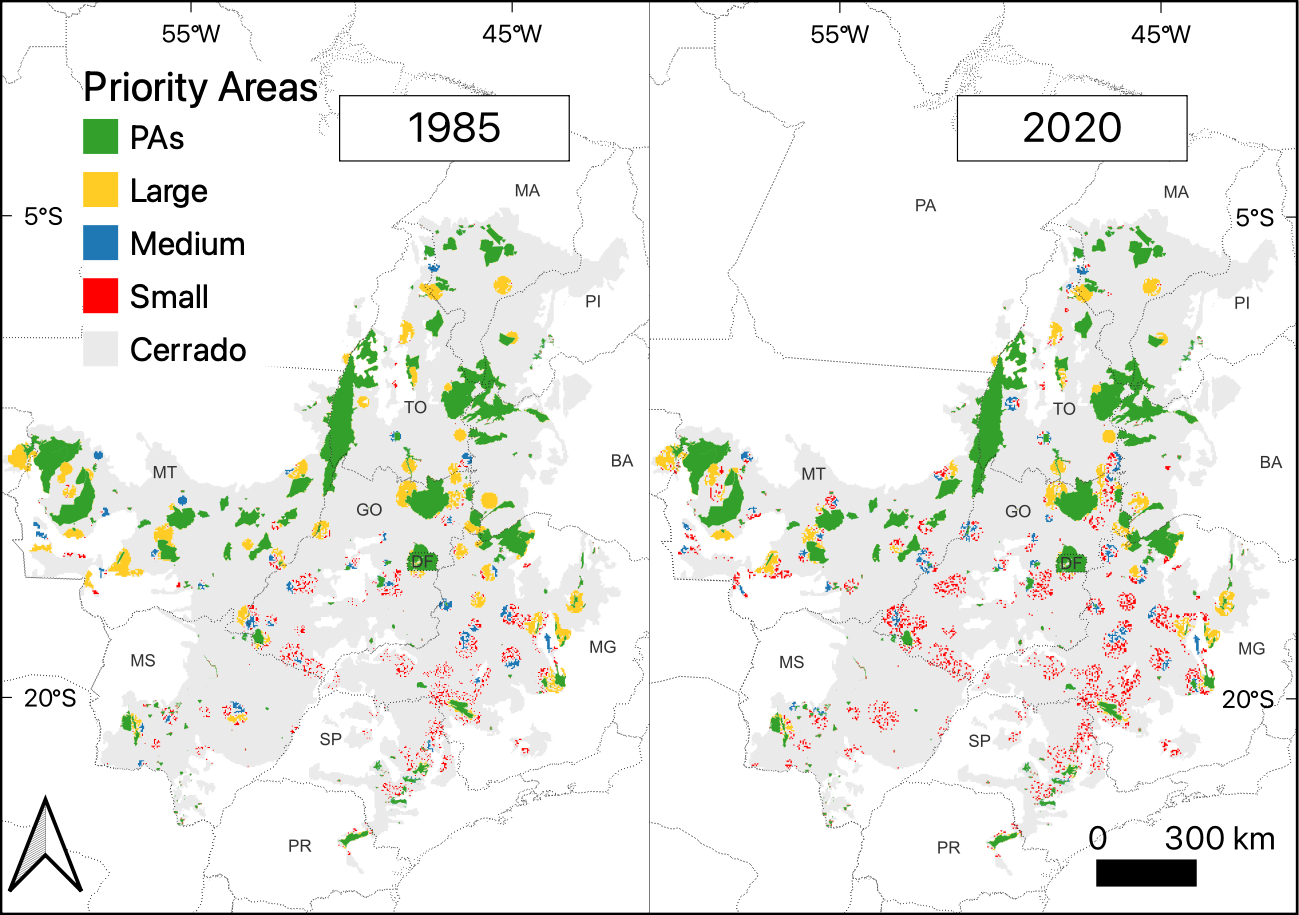
\includegraphics[width=160mm]{Fig c3-2}
	\caption[Top 17\% of the Cerrado ecoregion classified in distinct size categories]{\small Top 17\% of the Cerrado ecoregion for the conservation of endemic terrestrial vertebrate species, classified into three categories according to the territorial extension achieved upon the creation of protected areas. Thresholds considered were: over 1000 km\textsuperscript{2} for “Large” areas, and under 250 km\textsuperscript{2} for “Small” ones. Areas between 250 km\textsuperscript{2} and 1000 km\textsuperscript{2} were considered as “Medium”. State initials stand for: BA: Bahia; DF: Distrito Federal; GO: Goias; MA: Maranhao; MG: Minas Gerais; MS: Mato Grosso do Sul; MT: Mato Grosso; PA: Para; PI: Piaui; PR: Parana; SP: Sao Paulo and TO: Tocantins.}
	\label{fig:fig3-2}
\end{figure}

\begin{mdframed}[backgroundcolor=lightgray, linecolor=lightgray]
	\small \textbf{Box 1:} In Mato Grosso, priorities are to the northward expansion of the Chapada dos Guimarães National Park preferably aiming for the connection to the APA Cabeceiras do Rio Cuiabá. Our results also highlight the need to expand the Serra das Araras Ecological Station, and to implement new protected areas on the border and across the eastern portion of the Rondônia state coupled with the aim of connecting large extensions of indigenous lands in the westernmost limits of the Cerrado (\autoref{fig:fig3-2}). In Minas Gerais state, the focus should be given to the expansion and connection of the Sempre Vivas National Park with Rio Preto and Biribiri State Parks, as well as for the connection between the Grão Mogol and Botumirim State Parks with the Acauã Ecological Station. Our results also highlight an opportunity for great expansion around the Serra do Cabral State Park, a moderate expansion around the Serra da Canastra National Park, and the opportunity to create a large protected area in northwestern Minas Gerais, near the small Sagarana State Park (\autoref{fig:fig3-2}). In the northeastern portion of the Goiás state, at the border with Bahia, there is an opportunity to expand and connect the protected areas located at the Serra Geral plateau. As for northern Goiás and southern Tocantins, large extensions of natural habitat can be protected by the expansion of the Chapada dos Veadeiros National Park, and the APA Minaçu, aiming for connections with APA Pouso Alto in the east, and with APA Lago de São Salvador do Tocantins, Paranã and Palmeirópolis in the north (\autoref{fig:fig3-2}). Finally, for the northern portion of the Tocantins state our results highlight the opportunity to expand the APA Serra do Lageado; to expand the Árvores Fossilizadas Natural Monument aiding in the connection with the Chapada das Mesas National Park in eastern Maranhão state, and for the creation of a new protected area on the upper Tocantins river valley at the municipality of Guaraí. Notwithstanding, a large priority area is located in the municipality of Loreto in eastern Maranhão state, and an eastward expansion of Urucuí-Una Ecological Station in Piauí state is also amongst the top 17\% large priority areas (\autoref{fig:fig3-2}).
\end{mdframed}

The analyses of priority areas considering temporal series of LULC changes revealed a clear negative effect of postponing conservation action in the Cerrado. Opportunities to represent endemic terrestrial vertebrate distributions decreased with the conversion of natural habitats into anthropic uses (\autoref{tab:tab3-1}, \autoref{fig:fig3-3}). The average species distribution representation in large areas decreased as we compare the prioritization outcomes of recent land-use changes (from 17.3\% to 12.2\% in the 1985 and 2020 scenarios respectively, a difference of $\sim$ -5.1\%). On the contrary, the representation of species distributions in combined small and medium fragmented priority areas increased over time (from 7.4\% to 10.2\% in the 1985 and 2020 scenarios respectively, a difference of $\sim$ +2.8\%; \autoref{fig:fig3-3}).

\begin{table}[h]
	\centering
	\caption[Terrestrial vertebrate distribution representation in different land-use scenarios]{\small Percentage of endemic terrestrial vertebrate distribution representation in priority areas according to two targets of land protection in different scenarios of past land-use in the Brazilian Cerrado.}
	\label{tab:tab3-1}
	\vspace{\bigskipamount}
	\begin{tabular}{c c c}
		\hline
		\multicolumn{3}{c}{Representantion} \\
		\hline
		& Top 17\% & Top30\% \\
		\hline
		Pristine & 48.60\% & 73.66\% \\
		1985 & 45.58\% & 63.46\% \\
		1990 & 45.01\% & 61.34\% \\
		1995 & 44.49\% & 59.97\% \\
		2000 & 44.10\% & 58.78\% \\
		2005 & 43.95\% & 57.87\% \\
		2010 & 43.75\% & 57.21\% \\
		2015 & 43.82\% & 56.90\% \\
		2020 & 43.30\% & 55.84\% \\								
		\hline
	\end{tabular}
\end{table}

\begin{figure}[H]
	\centering
	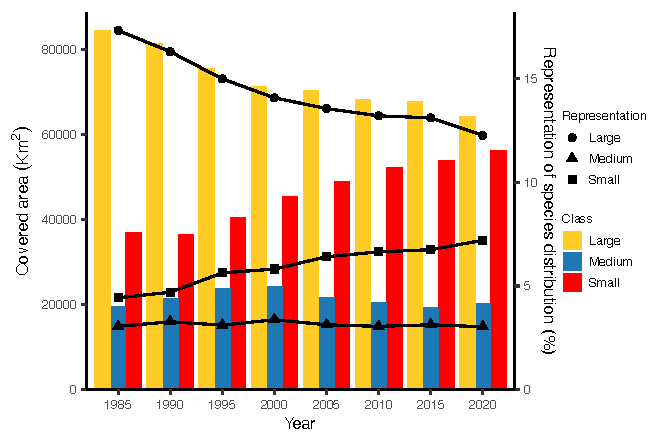
\includegraphics[width=160mm]{Fig c3-3}
	\caption[Changes in the total area covered by three different size categories of the top 17\% of the Cerrado ecoregion throughout time]{\small Changes in the total area covered by three different size categories of the top 17\% priority areas for the conservation of Cerrado endemic terrestrial vertebrate species throughout time and respective percentage of species distributions within each category. Thresholds considered were: over 1000 km\textsuperscript{2} for “Large” areas, and under 250 km\textsuperscript{2} for “Small” ones. Areas between 250 km\textsuperscript{2} and 1000 km\textsuperscript{2} were considered as “Medium”.}
	\label{fig:fig3-3}
\end{figure}
\section{Discussion}

In agreement with previous studies (\citealp[e.g.][]{PrietoTorres2020, PrietoTorres2022}), our findings suggest a suboptimal distribution of current Cerrado PAs. Considering that this region was pointed long ago as a biodiversity hotspot \citep{Myers2000} and is currently a deforestation frontier \citep{Pacheco2021}, strategic land-use planning is a pending issue that should be urgently addressed \citep{Strassburg2017, Lemes2020}. Otherwise, conservation opportunities will continue diminishing with the increase in habitat loss and fragmentation in these highly diverse savannas \citep{Nori2013, Resende2019}.

Herein we identified strategic areas to efficiently expand the Cerrado PA network. Most importantly, relatively small increments in the total protected area resulted in a significant increase in species representation. The 17\% land protection target was due in 2020 \citep{CBD2010} and has not been achieved yet, therefore the protection of the Brazilian Cerrado lags far behind the new ambitious target (30\%; \citealp{Woodley2019}). By comparing priority areas across different periods during the last decades, we pinpointed that habitat loss and fragmentation are the most important factors behind the rapid loss of conservation opportunities in the Cerrado (\citealp[see also][]{Grande2020}). While opportunities to increase the representation of species distributions did not decrease sharply over time, the top priority areas became smaller and fragmented as time passed. As a consequence, opportunities to represent species distributions in large priority areas (>1000 km\textsuperscript{2}) are decreasing as a result of the conversion of natural habitats into anthropic land use. Noteworthy, the increase in small and medium priority areas does not surpass the decrease of representation in larger ones, suggesting that the protection of large priority areas in the Cerrado should be more urgent than the protection of the smallest areas that have remained after the northward shift in the deforestation frontier \citep{Betts2017, deMarcoJr2020}.

Habitat connectivity in the Cerrado has decreased sharply during the last decades, mostly due to the loss of connecting fragments. Unfortunately, connectivity is being lost faster than the loss of natural habitats and we are close to a lower threshold of remaining habitats below which connectivity becomes severely compromised \citep{Grande2020}. Considering the habitat requirements of many of the species assessed here, large portions of connected natural environments are important to safeguard the maintenance of ecological processes \citep{Betts2017, Diaz2018}. The northern portion of the region encompasses the largest continuous priority areas even in the most recent and pessimistic land-use scenario. Worryingly, the Deforestation Front report \citep{Pacheco2021} highlights the northern portion of the Cerrado as the most impacted worldwide and forecasts a trend of persistent deforestation in the region. This evidence, coupled with our results, suggests a clear trend of further reduction of conservation opportunities if no actions are urgently taken to halt habitat loss in the Cerrado, especially in its northern portion \citep{Nori2013, Resende2019}. Although the small and isolated priority areas detected here might not be adequate for some of our target species (\citealp[see][]{deMarcoJr2020}), those located in the southern portion of the Cerrado are the last remaining habitat for many endemic vertebrate species studied herein and must not be overlooked.

Some regions of the northern portion of the Cerrado (e.g. Serra Geral plateau) remained climatically stable during the Quaternary climatic fluctuations \citep{Werneck2012}. This climatic stability conferred a conservation uniqueness in light of global climate change. Moreover, a study using a framework directed to halt vegetation loss combined with predictions of species distributions under climate change scenarios highlights priority areas for plant conservation in northern Cerrado \citep{Monteiro2020}, converging with our proposal, and others (\citealp[e.g.][]{Brum2019, DinizFilho2020, Pacheco2021}). For future scenarios, however, the southern portion of the Cerrado is hypothesized to be climatically stable \citep{deMarcoJr2020, DinizFilho2020}. So, the last remnants in the highly impacted southern portions should be preserved and reconnected via restoration activities \citep{Strassburg2017}. There is an opportunity to safeguard enough protection for species while also increasing agricultural production without impacting the remaining natural habitats in the Cerrado \citep{Strassburg2017}. This “greener scenario” and zero deforestation approach points also to the necessity of implementing restoration in critical areas, mostly in the southern portion of the ecoregion. In this sense, following our prioritization scheme and considering both the threat of current deforestation in northern Cerrado and the outstanding presence of discontinuous priority areas in the southern portion of the region \citep{Grande2020}, we propose the urgent implementation of new PAs on the northern Cerrado as the last chance to maintain naturally connected areas. In addition, the focus on restoration approaches should be directed towards the southern priority areas, especially those with the potential to be connected to compose conservation mosaics.

In fact, small and fragmented areas in southern Cerrado may serve as the backbone of larger conservation strategies focused on landscape connectivity and widespread, threatened species. Moreover, as most of our target species are relatively small-ranged and regionalized \citep{Nogueira2011, Azevedo2016}, given that creating large and continuous PAs is not a possibility, the question of conserving southern Cerrado endemics, is more of a problem of correctly locating PAs. Although small and highly fragmented, the few remaining Cerrado areas in the south are still home to hundreds of endemic vertebrate species studied herein. To lose more habitat in these areas would lead to very high extinction rates in the Cerrado, which would not be compensated by actions in the more connected and extensive northern areas. In agreement with previous biogeographical studies in the Cerrado, detecting complex, regionalized, and significantly co-distributed allopatric biotas \citep{Nogueira2011, Azevedo2016}, our priority areas span different portions of the Cerrado. Thus, resulting conservation strategies must adapt to each subregional land use context. In this sense, it is imperative to halt deforestation in the entire Cerrado, both in the highly fragmented south and in the current deforestation frontier in the north. Additionally, it would be essential to guarantee the representation of most of the Cerrado vegetational gradient as possible, since not only vascular plants (\citealp[see][]{Durigan2003}), but all endemic terrestrial vertebrate groups analyzed here (\citealp[e.g.][]{Nogueira2011, Valdujo2012, Carmignotto2022}) include habitat specialists depending on different habitats covering the Cerrado ecoregion, from gallery forest to savannas, woodlands, wetlands, and open grasslands.

The number of Data Deficient species and those not yet assessed by IUCN highlights a major knowledge shortfall that might hamper accurate policy-making in Cerrado. This implies that research investment aimed to fill knowledge gaps on these species could be considered a strategic investment to reach accurate conservation recommendations \citep{Nori2018, Nori2020}. Noteworthy more than half of the Cerrado endemic terrestrial vertebrate species classified as DD are amphibians (Appendix S3). It has been shown that most DD amphibians are facing a high extinction risk, especially in Brazil \citep{Morais2013}. Efforts to reduce the proportion of DD species on the IUCN redlist should be mandatory as this general “non-threatened” category is often overlooked by both the scientific community and decision-makers, leading to biased conservation recommendations \citep{Nori2018}.

Recent studies focused on the conservation of ecosystem services also highlight that time is critical for conserving the Brazilian Cerrado \citep{Resende2019}. Projections of land-use conversion under a business-as-usual scenario and forecasted extinctions in the next 30 years are clear proof that not only conservation policies should be immediately directed towards the protection of the Brazilian Cerrado, but also the whole cooperation of public and private sectors is necessary to achieve meaningful conservation results \citep{Strassburg2017}. If policy-making is not urgently focused on protecting strategic remnants of the Cerrado hotspot, halting habitat fragmentation, and using habitat restoration as a key activity (\citealp[see][]{Strassburg2017}), the future of the diverse endemic fauna of the central Brazilian savannas is clearly somber. However, the only way to achieve it will be through a joint effort of researchers, policy-makers, NGOs, and the private sector. In the era of delivery, not promises \citep{Loyola2022}, “tomorrow” might be too late.

\pagebreak

\section{Supporting information}\label{sec:supinfo-3}
\subsection*{Disclaimer}

A numeração dos apêndices 2 e 3 estão diferentes da do artigo original \citep{VieiraAlencar2023} em razão da inclusão do texto completo dos materiais e métodos (originalmente Appendix S2) diretamente na tese.

\subsection*{Appendix S1}\label{sup:3-s1}

\noindent
MapBiomas land-use and land-cover (LULC) classification and respective binary reclassification codes. Data were obtained and processed on Google Earth Engine, and the complete reclassification algorithm is available \href{https://code.earthengine.google.com/?scriptPath=users%2Fjoaosvalencar%2FJP%3APriority_Areas_2022}{here}

\begin{table}[H]
	\centering
	\caption*{}
	\label{tab:tab3-s1}
	\footnotesize
\begin{tabular}{c l c c}
	\hline
	Natural/Anthropic & Nomenclature & MapBiomas ID & Reclass Code \\
	\hline
	Mosaic & 1. Forest & 1 & 0 \\
	Natural & 1.1. Natural Forest & 3 & 0 \\
	Natural & 1.2. Savanna Formation & 4 & 0 \\
	Natural & 1.3. Mangrove & 5 & 0 \\
	Natural & 1.4. Wooded Restinga & 49 & 0 \\
	Mosaic & 2. Non Forest Natural Formation & 10 & 0 \\
	Natural & 2.1. Wetland & 11 & 0 \\
	Natural & 2.2. Grassland & 12 & 0 \\
	Natural & 2.3. Salt Flat & 32 & 0 \\
	Natural & 2.4. Rocky Outcrop & 29 & 0 \\
	Natural & 2.5. Other non Forest Formations & 13 & 0 \\
	Mosaic & 3. Farming & 14 & 1 \\
	Anthropic & 3.1. Pasture & 15 & 1 \\
	Anthropic & 3.2. Agriculture & 18 & 1 \\
	Anthropic & 3.2.1. Temporary Crop & 19 & 1 \\
	Anthropic & \quad 3.2.1.1. Soybean & 39 & 1 \\
	Anthropic & \quad 3.2.1.2. Sugar Cane & 20 & 1 \\
	Anthropic & \quad 3.2.1.3. Rice & 40 & 1 \\
	Anthropic & \quad 3.2.1.4. Other Temporary Crops & 41 & 1 \\
	Anthropic & 3.2.2. Perennial Crop & 36 & 1 \\
	Anthropic & \quad 3.2.2.1. Coffee & 46 & 1 \\
	Anthropic & \quad 3.2.2.2. Citrus & 47 & 1 \\
	Anthropic & \quad 3.2.2.3. Other Perennial Crop & 48 & 1 \\
	Anthropic & 3.3. Forest Plantation & 9 & 1 \\
	Anthropic & 3.4 Mosaic Agriculture and Pasture & 21 & 1 \\
	Mosaic & 4. Non-vegetated Area & 22 & 1 \\
	Natural & 4.1. Beach, Dune and Sand Spot & 23 & 0 \\
	Anthropic & 4.2. Urban Area & 24 & 1 \\
	Anthropic & 4.3. Mining & 30 & 1 \\
	Mosaic & 4.4. Other non Vegetated Areas & 25 & 1 \\
	Mosaic & 5. Water & 26 & 1 \\
	Mosaic & 5.1. River, Lake and Ocean & 33 & 1 \\
	Anthropic & 5.2. Aquaculture & 31 & 1 \\
	Non Identified & 6. Non-Observed & 27 & 1 \\
	\hline
\end{tabular}
\end{table}

\subsection*{Appendix S2}\label{sup:3-s2}

\noindent
Number of species of each terrestrial vertebrate group in each IUCN threat category. N = Absolute number; WG = percentages of each IUCN threat category within each terrestrial vertebrate group (column sum = 1); WC = percentages of each terrestrial vertebrate group within each IUCN threat category (WCs in one line sum = 1). Categories based on \citep{IUCN2022} are: LC = Least Concern; NT = Near Threatened; VU = Vulnerables; EN = Endangered; CR = Critically Endangered; DD = Data-Deficient; NA = Non-Assessed

\begin{table}[H]
	\centering
	\caption*{}
	\scriptsize
	\begin{tabular}{cccccccccccccccccccccccc}
		\hline
		& \multicolumn{3}{c}{Amphibians} && \multicolumn{3}{c}{Lizards} && \multicolumn{3}{c}{Snakes} && \multicolumn{3}{c}{Birds} && \multicolumn{3}{c}{Mammals} \\ \cline{2-4} \cline{6-8} \cline{10-12} \cline{14-16} \cline{18-20}
		Categories & N & WG & WC && N & WG & WC && N & WG & WC && N & WG & WC && N & WG & WC \\ 
		\hline
		LC & 41 & 0.33 & 0.28 && 34 & 0.52 & 0.23 && 36 & 0.56 & 0.24 && 20 & 0.45 & 0.14 && 16 & 0.41 & 0.11 \\
		NT & 2 & 0.02 & 0.13 && 2 & 0.03 & 0.13 && 1 & 0.02 & 0.07 && 8 & 0.18 & 0.54 && 2 & 0.05 & 0.13 \\
		VU & 0 & 0 & 0 && 2 & 0.03 & 0.12 && 5 & 0.08 & 0.29 && 9 & 0.2 & 0.53 && 1 & 0.03 & 0.06 \\
		EN & 0 & 0 & 0 && 3 & 0.05 & 0.2 && 2 & 0.03 & 0.14 && 5 & 0.11 & 0.33 && 5 & 0.13 & 0.33 \\
		CR & 3 & 0.02 & 0.43 && 2 & 0.03 & 0.29 && 1 & 0.02 & 0.14 && 1 & 0.02 & 0.14 && 0 & 0 & 0 \\
		DD & 36 & 0.29 & 0.57 && 10 & 0.15 & 0.16 && 8 & 0.13 & 0.13 && 0 & 0 & 0 && 7 & 0.18 & 0.14 \\
		NA & 42 & 0.34 & 0.56 && 13 & 0.2 & 0.17 && 10 & 0.16 & 0.13 && 2 & 0.04 & 0.03 && 8 & 0.2 & 0.11 \\
		 \hline
	\end{tabular}
\end{table}

\subsection*{Appendix S3}\label{sup:3-s3}

\noindent
Cerrado endemic terrestrial vertebrate species distribution representation in three distinct land protection thresholds. The proportion represented under each threshold considers the most recent land-use scenario available in \citet{MapBiomas2022}. PAs: Representation under current Cerrado’s protected area network; Top 17\%: Representation under the protection of the top 17\% of the land in the Cerrado; Top 30\%: Representation under the protection of the top 30\% of the land in the Cerrado.


\begin{longtable}{lccc}
	\hline
	&PAs&Top 17\%&Top 30\%\\
	\hline
	\endfirsthead
	\multicolumn{4}{r}%
	{\nameref{sup:3-s3} -- \textit{Continued from previous page}} \\
	\hline
	&PAs&Top 17\%&Top 30\%\\
	\hline
	\endhead
	\hline \multicolumn{4}{r}{\textit{Continued on next page}} \\
	\endfoot
	\hline
	\endlastfoot
	Average representation&21.47 &43.56 &56.18 \\
	\textit{Adenomera cotuba}&15.90 &28.40 &59.30 \\
	\textit{Adenomera saci}&26.30 &43.00 &57.20 \\
	\textit{Akodon kadiweu}&45.70 &67.90 &77.50 \\
	\textit{Akodon lindberghi}&44.40 &57.00 &62.60 \\
	\textit{Alectrurus tricolor}&22.90 &32.10 &41.60 \\
	\textit{Alipiopsitta xanthops}&12.40 &22.70 &38.60 \\
	\textit{Allobates brunneus}&21.50 &55.30 &74.20 \\
	\textit{Allobates goianus}&28.00 &51.50 &67.60 \\
	\textit{Alopoglossus collii}&19.70 &69.50 &71.50 \\
	\textit{Ameerega berohoka}&2.10 &18.00 &31.00 \\
	\textit{Ameerega braccata}&57.70 &77.30 &84.00 \\
	\textit{Ameerega flavopicta}&21.80 &38.00 &56.40 \\
	\textit{Ameerega picta}&18.80 &41.50 &57.80 \\
	\textit{Ameiva jacuba}&28.50 &41.10 &48.60 \\
	\textit{Ameiva parecis}&4.00 &77.60 &80.70 \\
	\textit{Ameivula cipoensis}&39.80 &70.50 &71.00 \\
	\textit{Ameivula jalapensis}&37.10 &59.40 &94.30 \\
	\textit{Ameivula mumbuca}&37.80 &50.30 &95.00 \\
	\textit{Ameivula xacriaba}&21.40 &33.00 &78.60 \\
	\textit{Amphisbaena absaberi}&5.50 &66.00 &66.50 \\
	\textit{Amphisbaena acrobeles}&92.80 &98.80 &100.00 \\
	\textit{Amphisbaena anaemariae}&26.20 &34.40 &44.20 \\
	\textit{Amphisbaena bedai}&3.40 &19.80 &31.20 \\
	\textit{Amphisbaena brevis}&15.20 &67.50 &74.30 \\
	\textit{Amphisbaena carli}&14.30 &36.90 &67.20 \\
	\textit{Amphisbaena crisae}&50.80 &62.50 &73.20 \\
	\textit{Amphisbaena cuiabana}&32.40 &43.90 &61.90 \\
	\textit{Amphisbaena filiformis}&3.70 &42.60 &77.20 \\
	\textit{Amphisbaena kraoh}&50.50 &61.60 &78.60 \\
	\textit{Amphisbaena leeseri}&1.70 &14.60 &27.60 \\
	\textit{Amphisbaena maranhensis}&0.70 &63.80 &93.10 \\
	\textit{Amphisbaena mebengokre}&0.00 &24.90 &26.80 \\
	\textit{Amphisbaena neglecta}&67.10 &81.80 &86.70 \\
	\textit{Amphisbaena persephone}&3.40 &56.00 &64.80 \\
	\textit{Amphisbaena sanctaeritae}&8.20 &21.80 &21.90 \\
	\textit{Amphisbaena saxosa}&55.40 &86.90 &88.80 \\
	\textit{Amphisbaena silvestrii}&20.30 &35.50 &51.70 \\
	\textit{Amphisbaena steindachneri}&7.70 &65.20 &65.90 \\
	\textit{Amphisbaena talisiae}&38.10 &52.30 &65.00 \\
	\textit{Anolis meridionalis}&20.60 &39.80 &53.40 \\
	\textit{Antilophia galeata}&15.20 &28.50 &41.70 \\
	\textit{Aplastodiscus lutzorum}&37.40 &45.30 &60.60 \\
	\textit{Apostolepis adhara}&10.60 &59.70 &86.90 \\
	\textit{Apostolepis albicollaris}&22.60 &39.20 &51.00 \\
	\textit{Apostolepis assimilis}&10.30 &21.70 &29.70 \\
	\textit{Apostolepis barrioi}&3.10 &14.30 &20.50 \\
	\textit{Apostolepis cerradoensis}&27.70 &78.30 &83.20 \\
	\textit{Apostolepis christineae}&10.90 &77.30 &80.20 \\
	\textit{Apostolepis flavotorquata}&28.20 &43.80 &52.70 \\
	\textit{Apostolepis goiasensis}&18.70 &35.00 &42.20 \\
	\textit{Apostolepis intermedia}&16.40 &28.30 &43.50 \\
	\textit{Apostolepis kikoi}&8.00 &55.00 &61.50 \\
	\textit{Apostolepis lineata}&67.10 &81.80 &86.70 \\
	\textit{Apostolepis longicaudata}&39.30 &49.40 &78.60 \\
	\textit{Apostolepis nelsonjorgei}&59.00 &75.90 &85.40 \\
	\textit{Apostolepis phillipsae}&14.90 &55.00 &55.00 \\
	\textit{Apostolepis polylepis}&31.30 &46.30 &71.30 \\
	\textit{Apostolepis sanctaeritae}&22.40 &35.60 &53.10 \\
	\textit{Apostolepis serrana}&7.00 &54.90 &57.20 \\
	\textit{Apostolepis striata}&21.70 &72.10 &73.10 \\
	\textit{Apostolepis tertulianobeui}&26.30 &52.00 &63.20 \\
	\textit{Apostolepis vittata}&31.30 &69.20 &74.90 \\
	\textit{Arremon flavirostris}&8.40 &19.80 &30.80 \\
	\textit{Asthenes luizae}&32.20 &65.70 &70.90 \\
	\textit{Atractus albuquerquei}&14.40 &36.90 &45.50 \\
	\textit{Atractus edioi}&18.20 &76.30 &86.70 \\
	\textit{Atractus pantostictus}&16.80 &35.60 &48.70 \\
	\textit{Atractus spinalis}&52.00 &78.30 &78.40 \\
	\textit{Atractus stygius}&3.50 &39.60 &64.70 \\
	\textit{Augastes scutatus}&20.20 &54.50 &65.90 \\
	\textit{Bachia bresslaui}&34.40 &47.20 &57.70 \\
	\textit{Bachia cacerensis}&11.20 &57.80 &58.20 \\
	\textit{Bachia didactyla}&23.50 &52.10 &59.20 \\
	\textit{Bachia geralista}&23.70 &41.80 &73.80 \\
	\textit{Bachia micromela}&0.00 &74.20 &79.50 \\
	\textit{Bachia oxyrhina}&67.50 &67.80 &92.60 \\
	\textit{Bachia psamophila}&38.60 &82.60 &83.50 \\
	\textit{Barycholos ternetzi}&12.90 &31.20 &52.60 \\
	\textit{Boana botumirim}&11.20 &66.90 &87.70 \\
	\textit{Boana buriti}&18.60 &37.50 &54.00 \\
	\textit{Boana caiapo}&17.10 &27.50 &41.40 \\
	\textit{Boana cipoensis}&18.80 &53.70 &70.60 \\
	\textit{Boana ericae}&82.90 &86.20 &95.70 \\
	\textit{Boana goiana}&33.90 &41.90 &61.50 \\
	\textit{Boana jaguariaivensis}&47.20 &61.40 &63.90 \\
	\textit{Boana lundii}&14.80 &30.60 &45.40 \\
	\textit{Boana stenocephala}&1.60 &25.70 &26.10 \\
	\textit{Bokermannohyla alvarengai}&22.50 &57.90 &71.30 \\
	\textit{Bokermannohyla ibitiguara}&30.20 &49.40 &50.40 \\
	\textit{Bokermannohyla izecksohni}&15.70 &29.80 &29.80 \\
	\textit{Bokermannohyla nanuzae}&19.60 &68.60 &71.70 \\
	\textit{Bokermannohyla napolii}&1.40 &25.90 &29.00 \\
	\textit{Bokermannohyla pseudopseudis}&47.30 &57.50 &76.50 \\
	\textit{Bokermannohyla ravida}&3.90 &33.00 &34.60 \\
	\textit{Bokermannohyla sagarana}&4.60 &55.40 &58.40 \\
	\textit{Bokermannohyla sapiranga}&27.60 &38.60 &54.90 \\
	\textit{Bokermannohyla saxicola}&18.50 &53.10 &67.70 \\
	\textit{Bokermannohyla sazimai}&8.20 &28.10 &32.30 \\
	\textit{Bothrops itapetiningae}&10.70 &19.50 &25.90 \\
	\textit{Bothrops marmoratus}&19.20 &33.70 &52.70 \\
	\textit{Bothrops moojeni}&8.50 &19.00 &30.10 \\
	\textit{Bothrops pauloensis}&7.80 &18.30 &24.90 \\
	\textit{Calassomys apicalis}&9.40 &62.20 &69.90 \\
	\textit{Callithrix penicillata}&18.80 &31.30 &42.50 \\
	\textit{Calomys tocantinsi}&34.20 &46.50 &63.60 \\
	\textit{Carterodon sulcidens}&27.00 &52.50 &62.40 \\
	\textit{Celeus obrieni}&8.80 &18.80 &42.80 \\
	\textit{Cercomacra ferdinandi}&26.50 &40.90 &69.20 \\
	\textit{Cerradomys akroai}&14.70 &52.20 &87.50 \\
	\textit{Cerradomys marinhus}&10.90 &26.60 &45.10 \\
	\textit{Cerradomys scotti}&21.40 &35.80 &50.60 \\
	\textit{Charitospiza eucosma}&15.80 &27.80 &44.00 \\
	\textit{Chiasmocleis albopunctata}&14.10 &35.90 &52.80 \\
	\textit{Chiasmocleis centralis}&4.60 &37.40 &41.50 \\
	\textit{Chironius brazili}&20.20 &38.20 &49.10 \\
	\textit{Cinclodes espinhacensis}&39.20 &67.60 &69.20 \\
	\textit{Clibanornis rectirostris}&7.70 &18.80 &31.60 \\
	\textit{Clyomys laticeps}&24.60 &39.50 &46.30 \\
	\textit{Coleodactylus brachystoma}&18.50 &40.00 &65.00 \\
	\textit{Colobosaura modesta}&21.90 &40.80 &57.10 \\
	\textit{Columbina cyanopis}&10.20 &41.10 &53.50 \\
	\textit{Conothraupis mesoleuca}&15.20 &34.70 &51.10 \\
	\textit{Coryphaspiza melanotis}&13.40 &25.80 &38.20 \\
	\textit{Crossodactylus franciscanus}&22.40 &40.80 &42.10 \\
	\textit{Crossodactylus trachystomus}&17.70 &58.70 &66.10 \\
	\textit{Ctenomys bicolor}&4.60 &32.80 &54.00 \\
	\textit{Ctenomys nattereri}&9.90 &49.00 &64.10 \\
	\textit{Cyanocorax cristatellus}&10.80 &22.00 &34.50 \\
	\textit{Dendropsophus anataliasiasi}&12.30 &26.60 &46.10 \\
	\textit{Dendropsophus araguaya}&2.10 &35.20 &40.00 \\
	\textit{Dendropsophus cerradensis}&2.50 &19.70 &20.20 \\
	\textit{Dendropsophus cruzi}&10.30 &29.90 &48.90 \\
	\textit{Dendropsophus elianeae}&8.60 &22.00 &31.30 \\
	\textit{Dendropsophus jimi}&9.90 &22.30 &31.00 \\
	\textit{Dendropsophus rhea}&9.10 &20.60 &20.70 \\
	\textit{Dendropsophus rubicundulus}&11.90 &27.50 &51.40 \\
	\textit{Dendropsophus tritaeniatus}&17.80 &32.70 &50.30 \\
	\textit{Drymoluber brazili}&10.50 &23.00 &31.50 \\
	\textit{Elachistocleis bumbameuboi}&13.30 &76.40 &93.40 \\
	\textit{Elachistocleis matogrosso}&12.50 &25.70 &51.70 \\
	\textit{Embernagra longicauda}&12.60 &40.90 &60.80 \\
	\textit{Enyalius capetinga}&36.40 &43.90 &67.30 \\
	\textit{Epicrates crassus}&12.00 &23.70 &36.50 \\
	\textit{Epictia clinorostris}&6.70 &28.60 &42.10 \\
	\textit{Erythrolamprus maryellenae}&40.90 &55.00 &66.20 \\
	\textit{Eurolophosaurus nanuzae}&25.90 &68.20 &70.90 \\
	\textit{Euryoryzomys lamia}&23.70 &37.80 &57.10 \\
	\textit{Euscarthmus rufomarginatus}&19.60 &29.20 &51.10 \\
	\textit{Galea flavidens}&26.00 &40.80 &55.60 \\
	\textit{Geositta poeciloptera}&23.70 &34.10 &46.30 \\
	\textit{Guyramemua affine}&27.80 &37.80 &54.20 \\
	\textit{Gyldenstolpia planaltensis}&58.80 &71.20 &77.60 \\
	\textit{Gymnodactylus amarali}&19.00 &36.30 &61.20 \\
	\textit{Gymnodactylus guttulatus}&15.50 &87.00 &88.30 \\
	\textit{Helicops boitata}&6.50 &43.40 &44.80 \\
	\textit{Helicops gomesi}&7.00 &12.10 &18.40 \\
	\textit{Helicops phantasma}&24.90 &47.30 &71.50 \\
	\textit{Herpsilochmus longirostris}&6.90 &15.60 &26.50 \\
	\textit{Heterodactylus lundii}&25.20 &54.00 &56.40 \\
	\textit{Holochilus sciureus}&14.70 &33.40 &52.10 \\
	\textit{Hoplocercus spinosus}&19.90 &36.10 &48.40 \\
	\textit{Hydropsalis candicans}&9.20 &22.20 &32.70 \\
	\textit{Hylodes otavioi}&36.50 &68.20 &68.50 \\
	\textit{Ischnocnema penaxavantinho}&0.80 &25.10 &31.80 \\
	\textit{Kentropyx paulensis}&25.30 &38.20 &48.30 \\
	\textit{Kentropyx vanzoi}&18.50 &48.70 &59.40 \\
	\textit{Kerodon acrobata}&8.80 &40.30 &59.00 \\
	\textit{Knipolegus franciscanus}&12.60 &26.60 &48.70 \\
	\textit{Kunsia tomentosus}&24.30 &60.60 &62.70 \\
	\textit{Laterallus xenopterus}&11.10 &19.40 &35.80 \\
	\textit{Leposternon cerradensis}&3.10 &19.80 &20.00 \\
	\textit{Leposternon maximus}&38.70 &48.30 &75.30 \\
	\textit{Leposternon mineiro}&0.00 &30.30 &41.60 \\
	\textit{Leptodactylus brevipes}&15.90 &29.60 &52.90 \\
	\textit{Leptodactylus camaquara}&22.70 &59.20 &78.20 \\
	\textit{Leptodactylus cunicularius}&27.20 &67.30 &68.80 \\
	\textit{Leptodactylus furnarius}&17.40 &39.50 &48.40 \\
	\textit{Leptodactylus kilombo}&0.80 &31.40 &48.70 \\
	\textit{Leptodactylus pustulatus}&8.80 &26.50 &48.20 \\
	\textit{Leptodactylus sertanejo}&28.10 &44.40 &59.90 \\
	\textit{Leptodactylus tapiti}&84.20 &87.50 &93.80 \\
	\textit{Liotyphlops schubarti}&3.80 &23.70 &24.20 \\
	\textit{Liotyphlops taylori}&10.90 &77.30 &80.20 \\
	\textit{Lonchophylla bokermanni}&43.20 &81.50 &81.80 \\
	\textit{Lonchophylla dekeyseri}&38.30 &47.50 &61.40 \\
	\textit{Lycalopex vetulus}&18.20 &32.40 &45.00 \\
	\textit{Lygophis paucidens}&36.10 &49.30 &67.80 \\
	\textit{Lysapsus caraya}&29.80 &39.90 &57.10 \\
	\textit{Manciola guaporicola}&32.10 &50.80 &61.20 \\
	\textit{Melanopareia torquata}&19.40 &33.40 &47.20 \\
	\textit{Micrablepharus atticolus}&19.40 &38.30 &51.20 \\
	\textit{Microakodontomys transitorius}&59.70 &68.30 &73.60 \\
	\textit{Microspingus cinereus}&17.20 &35.20 &50.20 \\
	\textit{Micrurus brasiliensis}&32.70 &48.50 &68.50 \\
	\textit{Micrurus tricolor}&7.80 &18.00 &39.30 \\
	\textit{Monodelphis kunsi}&15.40 &34.50 &48.50 \\
	\textit{Monodelphis sanctaerosae}&10.40 &61.30 &68.20 \\
	\textit{Myiothlypis leucophrys}&17.60 &27.70 &39.40 \\
	\textit{Neothraupis fasciata}&18.40 &31.00 &46.60 \\
	\textit{Nothura minor}&22.20 &33.90 &41.00 \\
	\textit{Nyctiprogne vielliardi}&5.90 &30.50 &45.20 \\
	\textit{Nystalus striatipectus}&3.10 &11.40 &27.80 \\
	\textit{Odontophrynus cultripes}&13.60 &28.60 &40.10 \\
	\textit{Odontophrynus juquinha}&17.00 &57.80 &68.40 \\
	\textit{Odontophrynus monachus}&31.80 &50.90 &51.60 \\
	\textit{Oecomys cleberi}&15.50 &26.20 &36.90 \\
	\textit{Oligoryzomys moojeni}&25.50 &42.90 &72.80 \\
	\textit{Oligoryzomys rupestris}&79.90 &91.10 &91.40 \\
	\textit{Oreobates antrum}&18.70 &40.70 &53.60 \\
	\textit{Oreobates heterodactylus}&24.80 &52.50 &73.70 \\
	\textit{Oreobates remotus}&50.60 &78.80 &88.00 \\
	\textit{Oxymycterus delator}&39.20 &51.10 &63.40 \\
	\textit{Oxymycterus itapeby}&46.60 &60.60 &63.20 \\
	\textit{Paroaria baeri}&25.70 &33.70 &48.30 \\
	\textit{Penelope ochrogaster}&14.70 &28.90 &50.30 \\
	\textit{Phaethornis nattereri}&12.80 &26.40 &42.20 \\
	\textit{Phalotris cerradensis}&37.90 &64.70 &87.30 \\
	\textit{Phalotris concolor}&1.80 &39.50 &56.20 \\
	\textit{Phalotris labiomaculatus}&25.60 &52.10 &83.20 \\
	\textit{Phalotris lativittatus}&5.70 &16.90 &21.00 \\
	\textit{Phalotris matogrossensis}&4.90 &18.20 &29.50 \\
	\textit{Phalotris mertensi}&5.80 &13.60 &18.80 \\
	\textit{Phalotris multipunctatus}&13.60 &28.20 &28.80 \\
	\textit{Phalotris nasutus}&14.00 &24.80 &33.70 \\
	\textit{Phasmahyla jandaia}&19.00 &53.00 &66.20 \\
	\textit{Philodryas livida}&16.70 &30.40 &35.70 \\
	\textit{Philodryas mattogrossensis}&2.40 &14.90 &22.60 \\
	\textit{Phyllomyias reiseri}&16.00 &30.00 &49.70 \\
	\textit{Phyllomys brasiliensis}&6.20 &38.00 &41.50 \\
	\textit{Phyllomys centralis}&45.70 &64.90 &66.30 \\
	\textit{Phylloscartes roquettei}&7.20 &21.90 &44.10 \\
	\textit{Physalaemus atim}&13.10 &33.10 &34.70 \\
	\textit{Physalaemus centralis}&12.80 &28.80 &45.80 \\
	\textit{Physalaemus claptoni}&42.50 &75.20 &75.40 \\
	\textit{Physalaemus deimaticus}&27.90 &68.70 &69.00 \\
	\textit{Physalaemus evangelistai}&23.90 &71.10 &74.30 \\
	\textit{Physalaemus marmoratus}&11.20 &25.90 &39.60 \\
	\textit{Physalaemus nattereri}&7.80 &21.30 &36.60 \\
	\textit{Pithecopus araguaius}&23.60 &41.80 &67.00 \\
	\textit{Pithecopus ayeaye}&18.30 &38.30 &42.30 \\
	\textit{Pithecopus azureus}&12.90 &31.90 &53.80 \\
	\textit{Pithecopus centralis}&41.20 &67.10 &76.40 \\
	\textit{Pithecopus megacephalus}&22.40 &60.70 &74.10 \\
	\textit{Pithecopus oreades}&59.00 &69.30 &77.90 \\
	\textit{Placosoma cipoense}&49.00 &76.70 &76.70 \\
	\textit{Polystictus superciliaris}&18.30 &45.40 &58.10 \\
	\textit{Porphyrospiza caerulescens}&16.50 &31.40 &49.60 \\
	\textit{Pristimantis dundeei}&21.90 &38.80 &56.30 \\
	\textit{Pristimantis moa}&7.10 &30.20 &77.80 \\
	\textit{Pristimantis ventrigranulosus}&5.30 &28.90 &36.50 \\
	\textit{Proceratophrys bagnoi}&18.80 &57.30 &79.50 \\
	\textit{Proceratophrys branti}&22.90 &41.50 &68.30 \\
	\textit{Proceratophrys carranca}&0.00 &35.00 &39.10 \\
	\textit{Proceratophrys cururu}&34.90 &73.20 &75.10 \\
	\textit{Proceratophrys dibernardoi}&1.00 &17.70 &28.50 \\
	\textit{Proceratophrys goyana}&18.70 &33.50 &57.60 \\
	\textit{Proceratophrys huntingtoni}&14.50 &47.60 &62.80 \\
	\textit{Proceratophrys moratoi}&8.30 &18.80 &25.50 \\
	\textit{Proceratophrys rotundipalpebra}&84.60 &87.30 &95.20 \\
	\textit{Proceratophrys salvatori}&44.60 &52.50 &66.40 \\
	\textit{Proceratophrys strussmannae}&3.40 &69.20 &79.10 \\
	\textit{Proceratophrys vielliardi}&26.50 &34.60 &51.80 \\
	\textit{Pseudis tocantins}&10.50 &24.90 &51.50 \\
	\textit{Pseudopaludicola atragula}&1.80 &15.80 &16.60 \\
	\textit{Pseudopaludicola coracoralinae}&2.80 &23.50 &24.80 \\
	\textit{Pseudopaludicola facureae}&0.50 &10.80 &16.60 \\
	\textit{Pseudopaludicola ibisoroca}&2.00 &29.80 &35.90 \\
	\textit{Pseudopaludicola jazmynmcdonaldae}&56.40 &85.70 &87.70 \\
	\textit{Pseudopaludicola mineira}&25.30 &66.20 &67.30 \\
	\textit{Pseudopaludicola ternetzi}&18.20 &30.00 &44.50 \\
	\textit{Psilops seductus}&22.90 &57.00 &76.60 \\
	\textit{Pyrrhura pfrimeri}&15.80 &38.80 &52.60 \\
	\textit{Rhachidelus brazili}&8.70 &17.10 &25.60 \\
	\textit{Rhachisaurus brachylepis}&22.70 &59.50 &72.00 \\
	\textit{Rhinella cerradensis}&16.20 &25.80 &56.40 \\
	\textit{Rhinella inopina}&21.10 &43.30 &64.70 \\
	\textit{Rhinella ocellata}&24.50 &40.60 &56.80 \\
	\textit{Rhinella rubescens}&20.00 &38.70 &52.10 \\
	\textit{Rhinella scitula}&14.90 &33.80 &49.40 \\
	\textit{Rhinella sebbeni}&16.50 &29.70 &42.50 \\
	\textit{Rhinella veredas}&7.70 &16.80 &63.20 \\
	\textit{Rhipidomys ipukensis}&18.30 &42.70 &68.30 \\
	\textit{Rhipidomys macrurus}&26.60 &38.40 &54.50 \\
	\textit{Saltatricula atricollis}&10.80 &22.10 &36.70 \\
	\textit{Salvator duseni}&46.70 &56.80 &69.70 \\
	\textit{Scinax cabralensis}&6.60 &52.10 &52.80 \\
	\textit{Scinax canastrensis}&12.50 &30.20 &36.10 \\
	\textit{Scinax centralis}&7.30 &22.20 &34.90 \\
	\textit{Scinax constrictus}&11.70 &23.90 &40.20 \\
	\textit{Scinax curicica}&25.30 &67.40 &76.70 \\
	\textit{Scinax goya}&23.30 &57.70 &73.60 \\
	\textit{Scinax haddadorum}&3.10 &31.60 &43.50 \\
	\textit{Scinax machadoi}&15.30 &54.90 &73.70 \\
	\textit{Scinax maracaya}&26.70 &46.80 &48.30 \\
	\textit{Scinax pinimus}&29.70 &63.70 &64.10 \\
	\textit{Scinax pombali}&25.70 &45.10 &47.80 \\
	\textit{Scinax rogerioi}&57.90 &62.30 &67.40 \\
	\textit{Scinax rossaferesae}&35.80 &48.20 &56.70 \\
	\textit{Scinax rupestris}&78.60 &83.90 &96.20 \\
	\textit{Scinax skaios}&22.40 &32.00 &55.00 \\
	\textit{Scinax tigrinus}&18.40 &31.40 &49.60 \\
	\textit{Scytalopus novacapitalis}&22.10 &34.30 &43.70 \\
	\textit{Siagonodon acutirostris}&59.80 &60.40 &87.80 \\
	\textit{Simophis rhinostoma}&7.40 &16.20 &23.00 \\
	\textit{Sporophila nigrorufa}&7.80 &41.80 &42.80 \\
	\textit{Stenocercus albolineatus}&6.10 &40.80 &52.40 \\
	\textit{Stenocercus canastra}&37.50 &56.70 &57.00 \\
	\textit{Stenocercus quinarius}&31.90 &42.70 &74.30 \\
	\textit{Stenocercus sinesaccus}&18.20 &45.90 &54.20 \\
	\textit{Synallaxis simoni}&11.50 &22.40 &39.40 \\
	\textit{Syndactyla dimidiata}&23.70 &34.00 &46.70 \\
	\textit{Taoniscus nanus}&32.40 &41.40 &51.70 \\
	\textit{Thalpomys cerradensis}&34.50 &56.30 &71.40 \\
	\textit{Thalpomys lasiotis}&54.70 &68.40 &74.30 \\
	\textit{Thamnodynastes rutilus}&28.70 &35.30 &47.40 \\
	\textit{Thoropa megatympanum}&21.60 &57.70 &72.30 \\
	\textit{Thrichomys apereoides}&9.10 &27.60 &50.40 \\
	\textit{Thrichomys pachyurus}&33.10 &44.70 &63.70 \\
	\textit{Thylamys velutinus}&45.10 &58.00 &61.00 \\
	\textit{Trachycephalus mambaiensis}&25.30 &39.30 &56.70 \\
	\textit{Trilepida brasiliensis}&14.90 &35.50 &59.40 \\
	\textit{Trilepida fuliginosa}&12.40 &23.40 &47.00 \\
	\textit{Trilepida jani}&14.50 &38.60 &62.20 \\
	\textit{Trilepida koppesi}&9.40 &19.90 &29.70 \\
	\textit{Trinomys moojeni}&33.30 &68.00 &68.40 \\
	\textit{Tropidophis preciosus}&1.00 &52.40 &53.70 \\
	\textit{Tropidurus callathelys}&20.50 &54.30 &54.50 \\
	\textit{Tropidurus chromatops}&16.10 &57.00 &57.40 \\
	\textit{Tropidurus itambere}&15.10 &28.20 &40.60 \\
	\textit{Tropidurus montanus}&13.40 &51.40 &62.70 \\
	\textit{Tropidurus oreadicus}&14.80 &32.60 &51.90 \\
	\textit{Tupinambis matipu}&23.80 &48.00 &60.60 \\
	\textit{Tupinambis quadrilineatus}&15.30 &27.50 &50.40 \\
	\textit{Uropelia campestris}&17.30 &30.10 &48.60 \\
	\textit{Vanzosaura savanicola}&30.00 &39.70 &72.30 \\
	\textit{Xenodon matogrossensis}&6.20 &21.30 &35.70 \\
	\textit{Xenodon nattereri}&10.80 &19.30 &28.60 \\
	
\end{longtable}

\addtocounter{table}{-1}

\chapter*[Conclusões Gerais]{Conclusões Gerais}

\addcontentsline{toc}{chapter}{Conclusões Gerais}

Ufa! Pra quem leu tudo (ou pelo menos um dos artigos acima) até aqui, o passeio foi longo, tortuoso (como as belas espécies de árvore do Cerrado) e complexo, né? Se não, que bom! Se sim, vamos lá para os principais pontos que precisam ser destacados e lembrados daqui.

Com nossos resultados, fica evidente que o conhecimento sobre a fauna de vertebrados terrestres endêmicos do Cerrado ainda tem um longo caminho pela frente. Desde o trabalho mais recente que compilou informações sobre anfíbios anuros e répteis Squamata endêmicos do Cerrado \citep{Azevedo2016}, 37 novas espécies foram descritas para esses grupos. Como esperado, a maioria das espécies descritas recentemente têm distribuições geográficas mais restritas, ou seja, podem não ter sido descritas anteriormente pelo simples fato de não terem sido nem mesmo encontradas antes, seja por raridade intrínseca, ou por que a região em que essas espécies ocorrem não haviam sido amostradas. Isso nos mostra que para uma região tão ampla e diversa como o Cerrado, mesmo com trabalhos recentes de levantamento faunístico sistemático voltados a reduzir lacunas de amostragem, ainda há muito espaço para avanço em conhecimento taxonômico (descrição de novas espécies) e biogeográfico (detalhamento sobre a distribuição geográfica das espécies). Em \citet{Azevedo2016} a base de dados analisada tinha 216 espécoes e 4588 registros únicos. Aqui, além das 37 espécies a mais de anfíbios anuros e de répteis Squamata adicionados à base, nós incluímos também registros de 45 espécies de aves e de 42 espécies de mamíferos. Com isso, nossa base de dados analisada chegou a 13.800 registros únicos, conferindo um aumento de 57\% em número de espécies e de 200\% em número de registros únicos analisados. Com essa síntese que fizemos pudemos encontrar alguns resultados interessantes e outros um tanto alarmantes.

Um ponto preocupante nesse cenário é que o ritmo de avanço sobre conhecimento taxonômico e biogeográfico não tem sido acompanhado por ações concretas direcionadas especificamente à proteção dessas espécies, mesmo diante do cenário preocupante de perda de hábitat, nem por refinamento em escala local e global sobre as avaliações do risco de extinção dessas espécies. Quase 87\% das espécies analisadas tiveram parte da área de suas distribuições geográficas modificadas de ambientes naturais para usos antrópicos, isso só no período entre o ano 2000 e 2020, com espécies que chegaram a perder até 45\% de toda sua área de distribuição. Para espécies que naturalmente possuem distribuições restritas a pequenas áreas do globo, perder qualquer quantidade de área natural dentro de suas áreas de distribuição já é preocupante. Considerando que muitas espécies endêmicas do Cerrado tem alta seletividade de hábitat, ou seja, ocupam majoritariamente um ou outro tipo de vegetação típico do Cerrado, essas perdas podem ser ainda mais significativas, especialmente se foram direcionadas ao habitat natural mais ligado a ocorrência dessas espécies. De modo geral, essa situação é mais complicada para espécies que originalmente ocorrem na porção sul do Cerrado. Isso porque nos anos 2000, quando foi publicado o trabalho clássico sobre hotspots de biodiversidade \citep{Myers2000} essa região já havia sido amplamente modificada. Por outro lado, apesar de encontrarmos que as espécies restritas à porção norte do Cerrado tem proporcionalmente mais áreas de habitat natural remanescentes em suas distribuições geográficas, é nessa região onde a chapa vem esquentando nos últimos anos, com as maiores taxas de desmatamento recentes. É nesse sentido que tanto no primeiro quando no terceiro capítulo nós chamamos a atenção para a necessidade de ampliar e criar novas unidades de conservação em porções específicas no Cerrado norte, mas sem deixar de lado a importância de tentar manter os remanescentes do Cerrado sul, propondo a criação de novas unidades de conservação que incluam planejamento de restauração integrado ao projeto de criação.

Somado a essa questão da alta perda de habitat recente, encontramos que mais de 87\% das espécies analisadas não tem nem 17\% da suas áreas de distribuição protegidas pela rede atual de unidades de conservação de uso restrito. Esses 17\%, são usados como parâmetro por que são o “alvo” que foi estipulado na convenção sobre diversidade biológica (\citeauthor{CBD2010}, da sigla em inglês para \textit{Convension on Biological Diversity}) que fosse protegido, do ambiente terrestre global até o ano de 2020. No Cerrado estamos distantes desse alvo e apenas 10,25\% são protegidos por lei, isso se considerarmos todas as categorias de unidade de conservação existentes, o que cai pra pouco mais de 2,5\% se considerarmos apenas as unidades de conservação de uso restrito. Como se isso não bastasse, encontramos no capitulo 3 que a conversão de áreas naturais ao longo dos anos vem reduzindo nossa capacidade de representar, proporcionalmente, maiores áreas da distribuição das espécies analisadas em áreas prioritárias à conservação, isso por que estamos consideramos aqui que ao converter uma área natural para qualquer uso do solo antrópico impede a ocorrência das espécies estudadas. Isso é fato para a maioria das espécies analisadas, porém nosso conhecimento sobre os hábitats preferenciais de algumas dessas espécies ainda é muito limitado, especialmente para espécies que foram descritas a partir de um único indivíduo ou de uma população de uma única localidade.

É nessa onda de que ainda precisamos coletar mais informações sobre algumas espécies que é possível justificar (mas não muito, veja a seguir) a alta quantidade de espécies avaliadas como possuindo “Dados Insuficientes” (espécies ‘\textit{DD - Data Deficient}’, de acordo com a nomenclatura usada pela União Internacional para Conservação da Natureza, a \citeauthor{IUCN2023}, da sigla em inglês para \textit{International Union for Conservation of Nature and Natural Resources}). Isso pra dizer que sim, de fato é interessante obter mais informações sobre as espécies descritas mais recentemente, porém, é de suma importância que avaliemos com mais atenção o que vem acontecendo em grande proporção dentro das distribuições dessas espécies, uma vez que especialmente espécies descritas mais recentemente, com distribuições restritas e com altas taxas de perda de habitat estão atualmente classificadas como ‘DD’ (ver “\autoref{fig:fig1-5}”), e isso dificulta a atribuição de pesos adequados à realidade de ameaça dessas espécies em análises sistemáticas de avaliação.

Ainda no que diz respeito a avaliação de risco de extinção das espécies analisadas, encontramos discrepâncias importantes entre a lista global e a lista nacional de espécies ameaçadas. Em primeiro lugar, na quantidade de espécies avaliadas em cada lista. A lista nacional é mais completa, contendo quase 93\% de todas as espécies conhecidas de tetrapoda endêmicas do Cerrado, em comparação com os quase 78\% da lista global. É preocupante que de modo geral temos mais espécies consideradas ameaçadas pela lista nacional, uma vez que é a lista global que normalmente é útilizada como referência em análises de priorização. Como, na prática, é possível que a lista global seja atualizada baseada nas listas nacionais, especialmente para espécies endêmica do Cerrado, que tem mais de 95\% da sua área contida em território brasileiro, essa diferença entre as duas listas pode resultar apenas da falta de celeridade na transferência de informações entre uma lista e outra, o que pode potencialmente ser solucionado com um melhor planejamento dessa etapa. Como possibilidade de análise futura, comparar os resultados de priorização pautados nas avaliações de cada lista poderá nos dar uma dimensão mais aproximada dos impactos que essa discrepância pode trazer no que diz respeito a determinação de áreas prioritárias à conservação, e talvez ressaltar a importância de sermos mais eficientes na comunicação entre as avaliações nacionais e a disponibilidade desses dados na lista global.

Ainda assim, comparando os resultados que nós encontramos com a proporção de espécies ameaçadas em cada classe de vertebrado em nivel global, é possível notar que mesmo a lista mais completa de avaliação (nesse caso, a lista nacional) pode nos limitar quando a interpretação correta sobre o risco de extinção das espécies analisadas. Isso por que não é nada trivial tentar explicar como as espécies endêmicas de um hotspot de biodiversidade, altamente impactado, também apontado como um hotspot de desmatamento recente, podem apresentar proporcionalmente menos espécies ameaçadas do que as espécies avaliadas em todo o globo. E foi isso o que encontramos. Se fossemos usar, por exemplo, a proporção de anfíbios ameaçados globalmente para ter uma estimativa conservadora de quantas espécies endêmicas de anfíbios poderiam, proporcionalmente, serem avaliadas como ameaçadas no Cerrado, deveríamos ter um número \textbf{DOZE} vezes maior de espécies avaliadas como ameaçadas. Se repetirmos esse raciocínio, para répteis Squamata deveríamos esperar pelo menos duas vezes e meia mais espécies avaliadas como ameaçadas. Desse modo, é possível apontar que há, potencialmente, alguma limitação considerável em avaliar adequadamente o risco de extinção das espécies da herpetofauna endêmica do Cerrado. Menciono especificamente a herpetofauna por que para aves e mamíferos a proporção de espécies avaliadas como ameaçadas no Cerrado é maior do que a encontrada para todas as espécies avaliadas no globo, o que condiz com condição de hotspot de biodiversidade, altamente impactado e com taxas crescentes de desmatamento.

Agora, sobre alguns avanços que tivemos e que podem nos ajudar a ter uma visão mais holística da composição de biotas formadas por espécies endêmicas do Cerrado. Apesar da sequência de capítulos apresentada, as primeiras ideias que queríamos testar nesta tese são as que foram apresentadas no capítulo 2, relacionadas aos resultados encontrados por \citet{Azevedo}. Isso para testar a robustez das unidades biogeográficas que foram encontradas naquele estudo, pensando que se essas unidades se mantivessem presentes com esse aumento no número de espécies e registros analisados, teríamos um sinal de que de fato essas poderiam ser consideradas válidas (pelo menos até o momento). No resumo da ópera, nós também encontramos um padrão de endemismo congruente a partir da detecção de clusters não aleatórios da distribuição de espécies co-distribuídas, mas, agora para tetrapoda. Além disso, 81\% das unidades detectadas por \citep{Azevedo2016} foram recuperadas com os nossos dados, e as que não foram detectadas certamente ficaram de fora por que algumas das espécies que às compunham não são mais consideradas espécies válidas, e essas unidades perderam o sinal biogeográfico que elas traziam. Por outro lado, nós detectamos novas unidades que ainda não haviam sido encontradas, como por exemplo as unidades da Bodoquena, os Campos Gerais no estado do Paraná e a da porção superior do vale do Rio Guaporé. E o que essas unidades têm em comum para terem sido encontradas dessa vez? Em primeiro lugar, todas elas tem pelo menos uma espécie de mamífero na sua composição, e em segundo, duas delas têm também espécies da herpetofauna descritas nos últimos anos. 

Isso nos mostra que, de fato, para chegarmos em algum ponto em que possamos propor unidades biogeográficas gerais e robustas, é importante tentar avaliar o maior número de espécies que tenhamos informações sobre suas distribuições, independente dessas espécies terem capacidades distintas de dispersão ou tolerâncias diferentes ao ambiente. E isso se reforça ao percebermos que mesmo as aves, que entre os grupos analisados têm a maior capacidade de dispersão, também são afetadas por fatores históricos que limitam a distribuição das espécies no Cerrado. Basta perceber que pelo menos um quarto das espécies de aves que formam as unidades detectadas estão em unidades classificadas como possuindo espécies de distribuições restritas e um terço formam unidades de distribuições parciais. Outro componente importante desse capítulo é o fato de que essas unidades biogeográficas são formadas majoritariamente ou por espécies com distribuicão altitudinal confinada nos planaltos ou confinadas nas depressões periféricas que permeiam o Cerrado, sendo que mais de 75\% de todas as espécies que formam as unidades detectadas estão em planaltos, incluindo mais de 85\% das espécies de aves e anfíbios. Com esse entendimento mais refinado sobre a composição, e localização das unidades, além da clara detecção do componente altitudinal na sua formação, temos maiores possibilidades de explorar perguntas relacionadas a delimitação dessas áreas, além de poder elaborar novos questionamentos sobre os processos envolvidos na formação da fauna endêmica e na origem do próprio Cerrado.

Pra finalizar, reconhecendo a problemática relacionada às ameaças intrínsecas (e.g. distribuições restritas e seletividade de hábitats) e extrínsecas (e.g. alta perda de hábitat, baixa taxa de proteção) das espécies analisadas é que fechamos a tese com um capítulo com a proposição de áreas prioritárias à conservação. Originalmente, áreas que seriam prioritárias à conservação de vertebrados terrestres endêmicos do Cerrado eram espalhadas por todo seu território e formadas por áreas de habitat natural contíguas. Com o passar do tempo e com estímulos para que a região central do Brasil fosse ocupada e utilizada para o desenvolvimento econômico do país, especialmente através da agropecuária, grandes extensões de hábitats naturais foram convertidas a usos antrópicos. Inicialmente esse processo acometeu principalmente a porção sul do Cerrado, de modo que já em 1985 uma vasta porção dessa região já havia sido convertida. Embora novas unidades de conservação tenham sido criadas ao longo do tempo (ver “\textit{\nameref{fig:fig1-s1}}”, a proporção de área protegida por elas segue não sendo muito representativa, enquanto que a expansão agropecuária se manteve em ritmos acelerados, atualmente acometendo a região norte do Cerrado. É nesse cenário em que as maiores áreas prioritárias à conservação da fauna de vertebrados terrestres endêmicos atualmente estão concentradas na porção norte da ecoregião. Com isso das modificações na disponibilidade de áreas naturais para criação de unidades de conservação contíguas nós avaliamos o quanto era possível seguir representando essas espécies mesmo em unidades menores, e o que encontramos é que na prática, não é somente a extensão de áreas prioritáras contíguas que vem se reduzindo, mas também nossa capacidade de representar adequadamente grandes proporções das distribuições geográficas das espécies analisadas.

Por outro lado, ainda podemos ser \textit{um pouco} otimistas. Se as áreas prioritárias que encontramos forem de fato usadas para pautar a criação de unidades de conservação em tempo hábil, ainda seremos capazes de representar em média 43,5\% das distribuições das espécies analisadas. Isso necessitando aumentar em apenas 6,75\% a cobertura de unidades de conservação do Cerrado (alcançando os 17\% que mencionei mais acima), o que representa aproximadamente 135.000km\textsuperscript{2} do seu território. Ainda assim, embora a média das áreas de distribuição que passariam a ser representadas seja relativamente alta, haveriam espécies com apenas 10\% de suas distribuições protegidas. Isso teria uma melhora significativa caso os top 30\% da região fossem protegidos por unidades de conservação, com uma média de 56,2\% das distribuições dessas espécies sendo representadas, e com pelo menos 16,6\% da distribuição de cada espécie sendo incluso nessas unidades de conservação (ver “\textit{\nameref{sup:3-s3}}”). O que preocupa nesse cenário é que com a taxa de desmatamento sendo mais alta que a resposta com criação de unidades de conservação essas áreas prioritárias seguirão sendo deterioradas e nossa capacidade de proteger essas espécies também. Por isso ressaltamos a necessidade de salvaguardar a áreas prioritárias com maiores extensões, localizadas no norte do Cerrado, que é onde o avanço da agropecuária é mais acentuado atualmente (\citealp[ver][]{Pacheco2021}). Um ponto adicional a se considerar aqui é sobre o potencial de áreas de proteção que deveriam ser mantidas em propriedades privadas. Caso essas áreas sejam adequadamente restauradas ao ponto de se manterem/tornarem habitáveis seria possível aumentar ainda mais a representatividade de espécies de vertebrados ameaçadas no Cerrado. Assim, ampliamos o nosso leque de abordagens, para além da criação e restauração de unidades de conservação, o que pelo menos em teoria dá um respiro a mais, apesar de que seguiria sendo necessário capacitar e ampliar os esforços para fiscalização e avaliação da eficiência dessas áreas.

Só um adendo ligeiro antes de fechar de vez. Você deve ter notado (ou não) que o número de espécies analisadas em cada artigo variou. Embora o total de espécies de tetrapoda endêmicas do Cerrado descritas até janeiro de 2021 seja mesmo 340, para algumas análises não foi possível incluir todas elas. Isso por que algumas das análises dependiam da disponibilidade de dados da base do MapBiomas, e nesse caso temos apenas dados para o Cerrado incluso no território brasileiro. Desse modo, duas espécies endêmicas que ocorrem no Cerrado boliviano (\textit{Hylaeamys acritus} e \textit{Juscelinomys huanchacae}) acabaram excluídas e isso determinou o número total de espécies e registros analisados em cada capítulo. Além dessas duas, perceba que no capítulo 3 nós excluímos também a espécie \textit{Juscelinomys candango} da análise, mas isso por que decidimos não incluir uma espécie que é considerada extinta (pela lista global) em uma análise de prioridades de conservação. De todo modo, esses percalços metodológicos destacam que nossa capacidade de gerar planos sistemáticos de conservação que consideram ecorregiões inteiras na extensão que tem o Cerrado pode não ser a melhor estratégia para contemplar algumas espécies, especialmente as que ocorrem em áreas marginais dessas ecorregiões. Além disso, destacamos o papel fundamental de listas nacionais, com olhar mais detalhado e dedicado à fauna e flora local, e a importância de criar iniciativas transfronteiríças para salvaguardar a biodiversidade.

É isso… o resumo do resumo é: aprendemos muito sobre a biodiversidade de vertebrados terrestres endêmicos do Cerrado nas últimas décadas, no entanto, estamos descobrindo espécies que mal estão sendo validadas e já estão sob elevada pressão antrópica em seus habitats confinados às suas distribuições restritas. Além disso, como as distribuições dessas espécies revelam um padrão de co-ocorrência, é possível que unidades biogeográficas inteiras, geradas por processos históricos, estejam sob risco de perderem suas espécies representativas. Logo, é possível que percamos os sinais biogeográficos que essas espécies nos fornecem e consequentemente perdemos nossa capacidade de entender de modo mais aprofundado a origem do Cerrado e de sua riquíssima fauna e flora. E, a menos que ajamos de forma planejada e célere vamos cada vez mais ser limitados na nossa capacidade de conter a extinção de diversas espécies de animais e plantas na maior e mais ameaçada savana do planeta. 


%%%%%
%END%%
%%%%%

\pagebreak

\nolinenumbers

% LISTAS
\listoffigures
\listoftables
\newpage

\bibliographystyle{apacite}
\bibliography{refs.bib}

\pagebreak

\begin{figure}
	\centering
	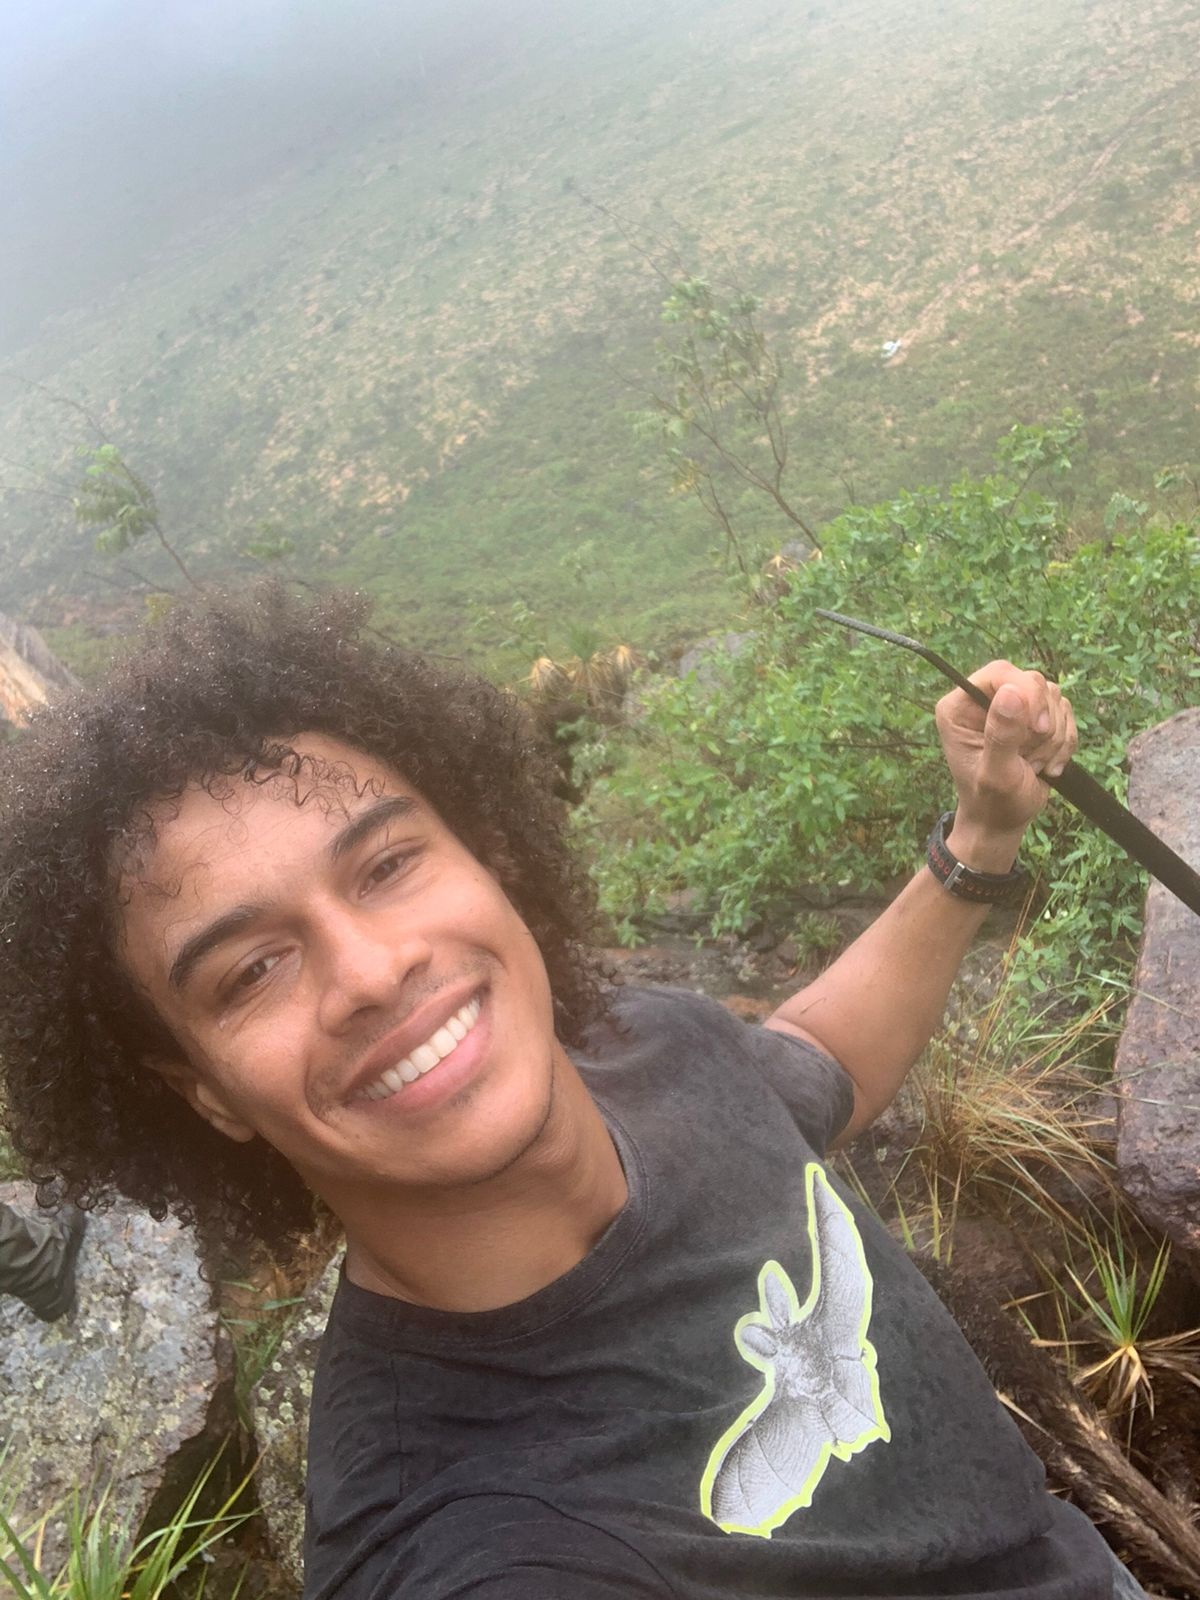
\includegraphics[width=160mm]{Fig JP}
	\caption*{\small Registro de um dia chuvoso no Morro do Fumo, localidade tipo da espécie de largarto endêmico \textit{Bachia oxyrhina} (10º51’58.41”S, 46º49’9.07”W), na Estação Ecológica Serra Geral do Tocantins.}
\end{figure}
\end{document}
